\documentclass[a4paper]{article}
\usepackage[T1]{fontenc}			% pacchetto per \chapter
\usepackage[italian]{babel}
\usepackage[italian]{isodate}  		% formato delle date in italiano
\usepackage{graphicx}				% gestione delle immagini
\usepackage{amsfonts}
\usepackage{booktabs}				% tabelle di qualità superiore
\usepackage{amsmath}				% pacchetto matematica
\usepackage{amsthm}					% teoremi migliorati
\usepackage{enumitem}				% gestione delle liste
\usepackage{pifont}					% pacchetto con elenchi carini
\usepackage{listings}				% pacchetto per i codici
\usepackage[x11names]{xcolor}		% pacchetto colori RGB
% Link ipertestuali per l'indice
\usepackage{xcolor}
\usepackage[linkcolor=black, citecolor=blue, urlcolor=cyan]{hyperref}
\hypersetup{
	colorlinks=true
}

\definecolor{codegreen}{rgb}{0,0.6,0}
\definecolor{codegray}{rgb}{0.5,0.5,0.5}
\definecolor{codepurple}{rgb}{0.58,0,0.82}
\definecolor{backcolour}{rgb}{0.95,0.95,0.92}
\lstdefinestyle{mystyle}{
	backgroundcolor=\color{backcolour},   
	commentstyle=\color{codegreen},
	keywordstyle=\color{magenta},
	numberstyle=\tiny\color{codegray},
	stringstyle=\color{codepurple},
	basicstyle=\ttfamily\footnotesize,
	breakatwhitespace=false,         
	breaklines=true,                 
	captionpos=b,                    
	keepspaces=true,                 
	numbers=left,                    
	numbersep=5pt,                  
	showspaces=false,                
	showstringspaces=false,
	showtabs=false,                  
	tabsize=2
}
\lstset{style=mystyle}

%\usepackage{showframe}				% visualizzazione bordi
%\usepackage{showkeys}				% visualizzazione etichetta

\newcommand{\longline}{\noindent\rule{\textwidth}{0.4pt}}
\newcommand{\dquotes}[1]{``#1''}
\renewcommand{\qedsymbol}{QED}

\begin{document}
	\author{VR443470}
	\title{Basi di dati}
	\date{\printdayoff\today}
	\maketitle

	\newpage
	
	% indice
	\tableofcontents
	
	\newpage
		
	\section{Introduzione}
	
	\subsection{Sistemi informativi, informazioni e dati}
	
	Ogni organizzazione è dotata di un \textbf{\emph{sistema informativo}}, che organizza e gestisce le informazioni necessarie per perseguire gli scopi dell'organizzazione stessa. Per indicare la \textbf{porzione automatizzata del sistema informativo} viene di solito utilizzato il termine \textbf{\emph{sistema informatico}}.
	
	Nei sistemi informatici le informazioni vengono rappresentate per mezzo di \emph{dati}, che hanno bisogno di essere interpretati per fornire informazioni. Esiste una differenza sottile tra dato e informazioni. Solitamente i primi, se presi da soli, non hanno significato, ma, una volta interpretati e correlati opportunamente, essi forniscono informazioni, che consentono di arricchire la conoscenza:

	\begin{description}
		\item[\textbf{Informazione}:] notizia, dato o elemento che consente di avere conoscenza più o meno esatta di fatti, situazioni, modi di essere;
		\item[\textbf{Dato}:] ciò che è immediatamente presente alla conoscenza, prima di ogni elaborazione. In informatica, sono elementi di informazione costituiti da simboli che devono essere elaborati.
	\end{description}
	
	\noindent
	\textcolor{Red3}{\textbf{[ESAME] Definizione base di dati}}: Una \textbf{\emph{base di dati}} è una collezione di dati, utilizzati per rappresentare con tecnologia informatica le informazioni di interesse per un sistema informativo.
	
	\newpage
	
	
	
	\subsection{Basi di dati e sistemi di gestione di basi di dati}
	
	Inizialmente, venne adottato un \dquotes{\underline{approccio convenzionale}} alla gestione dei dati. Esso \textbf{sfruttava} la presenza di archivi o \textbf{file per memorizzare} e \textbf{per ricercare dati}. Tuttavia, i metodi di accesso e condivisione erano semplici e banali.\newline
	Infatti, erano presenti numerosi \textbf{problemi}:
	
	\begin{itemize}
		\item[\ding{56}] \textbf{Accesso sequenziale}: la scarsa efficienza nell'accesso ai dati su file rendeva lento l'accesso a tali informazioni;
		\item[\ding{56}] \textbf{Ridondanza}: i dati di interesse per più programmi sono replicati tante volte quanti sono i programmi che li utilizzano, con evidente ridondanza e possibilità di incoerenza;
		\item[\ding{56}] \textbf{Inconsistenza}: una diretta conseguenza della ridondanza. Con la presenza di più copie di un determinato dato, l'eventuale cambiamento di uno solo potrebbe portare a questo effetto;
		\item[\ding{56}] \textbf{Progettazione duplicata}: per ogni programma viene replicata la progettazione.
	\end{itemize}
	
	\noindent
	La \textbf{soluzione} è arrivata negli anni '80 con l'avvento delle \textbf{basi di dati}. Quest'ultime gestiscono in modo integrato e flessibile le informazioni di interesse per diversi soggetti.\newline
	\newline \noindent	
	\textcolor{Red3}{\textbf{[ESAME] Definizione DBMS}}: Un \textbf{\emph{sistema di gestione di basi di dati}} (in inglese \emph{Data Base Management System}, \textbf{DBMS}) è un sistema software in grado di gestire collezioni di dati che siano:
	
	\begin{itemize}
		\item[\ding{52}] \textbf{Grandi};
		\item[\ding{52}] \textbf{Condivise};
		\item[\ding{52}] \textbf{Persistenti}.
	\end{itemize}
	
	\noindent
	\underline{assicurando} allo stesso tempo:
	
	\begin{itemize}
		\item[\ding{72}] \textbf{Affidabilità};
		\item[\ding{72}] \textbf{Privatezza};
		\item[\ding{72}] \textbf{Accesso efficiente}.
	\end{itemize}

	Il \textbf{vantaggio} di utilizzare un DBMS è stato evidenziato nella definizione. Quindi:
	
	\begin{itemize}
		\item[\ding{51}] \textbf{Maggiore astrazione} poiché le sue funzioni \underline{estendono il \emph{file system}}, fornendo la possibilità di accesso condiviso agli stessi dati da parte di più utenti e applicazioni;
		\item[\ding{51}] \textbf{Maggiore efficacia} poiché le operazioni di accesso ai dati si basano su un linguaggio di interrogazione.
	\end{itemize}
	
	
	
	
	\subsection{Linguaggi per basi di dati}
	Su un DBMS è possibile specificare operazioni di vario tipo, ma principalmente si distinguono in due categorie:

	\begin{itemize}
		\item \textbf{Linguaggi di definizione dei dati} (\emph{Data Definition Language}, abbreviato con \textbf{DDL}) utilizzati per \underline{definire} gli \underline{schemi logici}, \underline{esterni} e \underline{fisici} e le \underline{autorizzazioni per l'accesso};
		\item \textbf{Linguaggi di manipolazione dei dati} (\emph{Data Manipulation Language}, abbreviato con \textbf{DML}) \underline{utilizzati} per l'\underline{interrogazione} e l'\underline{aggiornamento} delle \underline{istanze} di basi di dati:
		\begin{itemize}
			\item \emph{Linguaggio di interrogazione}, estrae informazioni da una base di dati (SQL, algebra relazionale);
			\item \emph{Linguaggio di manipolazione}, popola la base di dati, modifica il suo contenuto con aggiunte, cancellazioni e variazioni sui dati (SQL).
		\end{itemize}
	\end{itemize}
	
	\newpage
	
	
	
	
	\subsection{Modelli dei dati}
	\textcolor{Red3}{\textbf{Definizione modello dei dati}}: Un \textbf{\emph{modello dei dati}} è un insieme di concetti utilizzati per organizzare i dati di interesse e descriverne la struttura in modo che essa risulti comprensibile ad un elaboratore.
	
	Ogni modello dei dati fornisce \textbf{meccanismi di strutturazione}, analoghi ai \textbf{\emph{costruttori}} di tipo dei linguaggi di programmazione (es: Java), che permettono di definire nuovi tipi sulla base di tipi predefiniti (elementari) e costruttori di tipo. Quindi, i \emph{costruttori} consentono di:
	
	\begin{itemize}
		\item[\ding{43}] \textbf{\emph{Definire}} le \textbf{strutture dati che conterranno le informazioni} della base di dati;
		\item[\ding{43}] \textbf{\emph{Specificare}} le \textbf{proprietà che dovranno soddisfare le istanze} di informazione che saranno contenuto nelle strutture dati.
	\end{itemize}

	\noindent \newline
	\textcolor{Red3}{\textbf{Definizione schemi e istanze}}: È molto importante distinguere gli \textbf{schemi} e le \textbf{istanze} dal concetto di modello dei dati:
	
	\begin{itemize}
		\item \textbf{\emph{Schema}}: parte \underline{invariante nel tempo}, è costituita dalle caratteristiche dei dati. In altre parole, è la descrizione della struttura e delle proprietà di una specifica base di dati fatta utilizzando i costrutti del modello dei dati;
		\item \textbf{\emph{Istanza} o \emph{stato}}: parte \underline{variabile nel tempo}, è costituita dai valori effettivi. Quest'ultimi, in un certo istante, popolano le strutture dati della base di dati.
	\end{itemize}

	\begin{figure}[!htp]
		\centering
		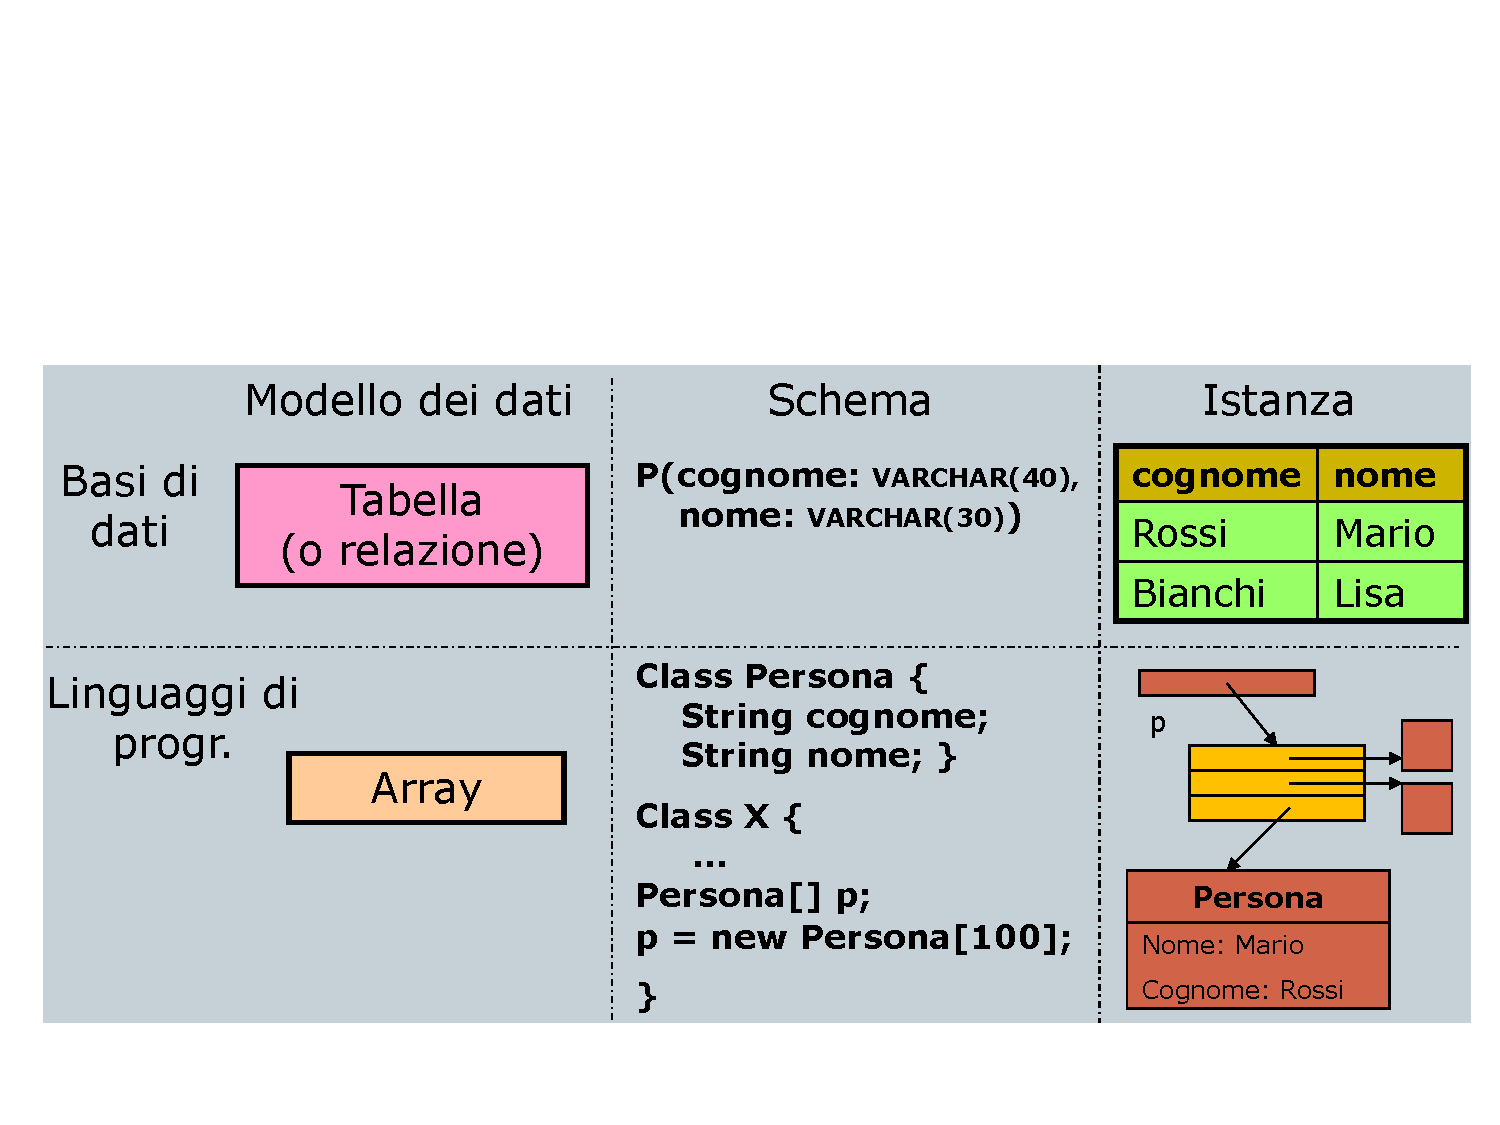
\includegraphics[width=0.9\textwidth]{img/diff_modello-schemi-istanze.pdf}
		\caption{Esempio di modello di dati, schema e istanza.}
	\end{figure}

	\newpage
	
	
	
	
	\subsection{Astrazione (architettura) dei DBMS}\label{Astrazione (architettura) dei DBMS}
	
	Esiste un'architettura standardizzata per i DMBS, la quale si caratterizza su tre livelli: \textbf{esterno}, \textbf{logico} e \textbf{interno}:
	
	\begin{itemize}
		\item[\ding{80}] \textbf{\emph{Schema logico.}} È la rappresentazione della \textbf{struttura} e delle \textbf{proprietà} della \textbf{base di dati} definita \underline{attraverso i costrutti} del modello dei dati del DBMS. In altre parole, descrive l'intera base di dati per mezzo del modello logico adottato dal DBMS (quindi relazione o ad oggetti).
		
		\item[\ding{72}] \textbf{\emph{Schema interno.}} È la rappresentazione della base di dati per mezzo delle \textbf{strutture fisiche di memorizzazione} (e.g. file sequenziale, file hash, ecc.).
		
		\item[\ding{73}] \textbf{\emph{Schema esterno.}}\label{schema esterno} Descrive una \textbf{porzione dello schema logico} di interesse per uno \textbf{specifico} utente o applicazione. \underline{Possono esistere più schemi} esterni che consentono di avere \underline{punti di vista differenti} senza cambiare la logica di base.
	\end{itemize}

	\begin{figure}[!htp]
		\centering
		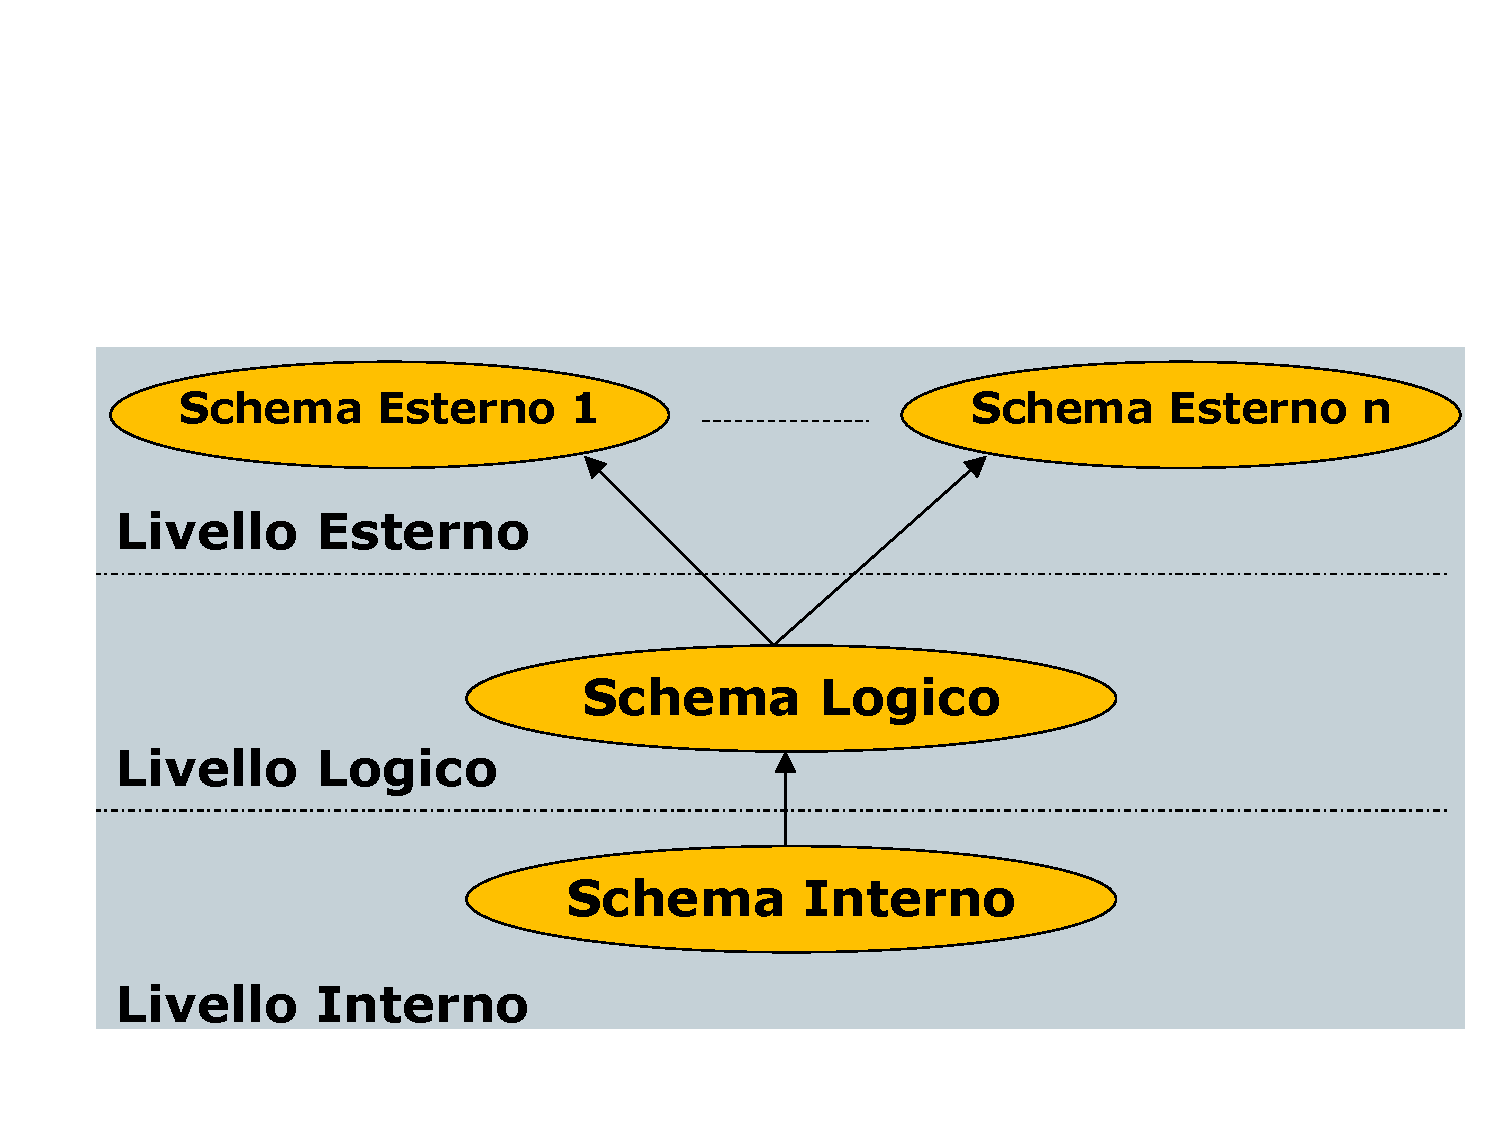
\includegraphics[width=0.8\textwidth]{img/arch_DBMS.pdf}
		\caption{Architettura generale di un DBMS.}
	\end{figure}

	\newpage
	
	
	
	
	\subsection{Indipendenza dei dati}
	
	L'architettura a livelli definita nel paragrafo \ref{Astrazione (architettura) dei DBMS} garantisce l' \textcolor{Red3}{\textbf{indipendenza dei dati}}, la \textbf{proprietà più importante} dei DBMS. L'\textbf{obbiettivo} è quello di poter fornire all'utente una basi di dati in grado di interagire con un \underline{elevato livello di astrazione}. Esistono due tipi di indipendenza:
	
	\begin{itemize}
		\item[\ding{42}] \textbf{\emph{Indipendenza \underline{fisica}.}} Lo schema logico della basi di dati è \underline{completamente} indipendente dallo schema interno. Quindi, l'interazione con il DBMS può essere effettuato in modo indipendente dalla struttura fisica dei dati.\newline
		\textcolor{Green4}{\textbf{Vantaggio:}} le modifiche \textbf{\underline{non}} influiscono sullo schema logico, cioè sulle applicazioni che lo utilizzano.
		
		\item[\ding{42}] \textbf{\emph{Indipendenza \underline{logica}.}} Gli \underline{schemi esterni} (definizione nel paragrafo:~\ref{schema esterno}) della base di dati sono \textbf{\underline{indipendenti}} dallo \underline{schema logico}. Quindi, è possibile interagire con il livello esterno in modo indipendente dal livello logico.\newline
		\textcolor{Green4}{\textbf{Vantaggio:}}
		\begin{enumerate}[label=\Roman*]
			\item \textbf{Aggiunta/Modifica} di uno schema \underline{esterno} in base alle esigenze di un nuovo utente, senza modificare lo schema logico;
			
			\item \textbf{Modifica} di uno schema logico mantenendo inalterate le strutture esterne.
		\end{enumerate}
	\end{itemize}

	\newpage
	
	


	\section{Metodologie e modelli per il progetto}
	
	\subsection{Ciclo di vita dei sistemi informativi}
	
	La progettazione di una base di dati costituisce solo una delle componenti del processo di sviluppo di un sistema informativo complesso e va quindi inquadrata in un contesto più ampio quello del \textbf{ciclo di vita} dei sistemi informativi:
	
	\begin{itemize}
		\item[\ding{42}] \textbf{\emph{Studio di fattibilità.}} Definisce i \underline{costi} delle varie alternative possibili e stabilisce le \underline{priorità di realizzazione} delle varie componenti del sistema.
		
		\item[\ding{42}] \textbf{\emph{Raccolta e analisi dei requisiti.}} Individua le proprietà e le funzionalità che il sistema informativo deve avere producendo una descrizione completa, ma generalmente informale.
		
		\item[\ding{42}] \textbf{\emph{Progettazione.}} Si divide in due fasi:
		\begin{itemize}
			\item \textbf{Progettazione dei dati.} Individua la struttura e l'organizzazione che i dati devono avere.
			
			\item \textbf{Progettazione delle applicazioni.} Definizione delle caratteristiche dei programmi applicativi.
		\end{itemize}
		
		\item[\ding{42}] \textbf{\emph{Implementazione (su un DBMS).}} È la realizzazione del sistema informativo secondo la struttura e le caratteristiche fornite durante la fase di progettazione. In questa fase \underline{viene costruita e popola la base di dati}.
		
		\item[\ding{42}] \textbf{\emph{Validazione e collaudo.}} Verifica il corretto funzionamento e la qualità del sistema informativo.
		
		\item[\ding{42}] \textbf{\emph{Funzionamento.}} Il sistema informativo diventa operativo ed esegue i compiti per i quali è stato progettato.
	\end{itemize}

	\noindent
	Spesso il processo \textbf{non} è strettamente sequenziale. Infatti, come si vede dalla seguente figura, durante l'esecuzione di una delle attività sopraelencate, è necessario rivedere decisioni prese nell'attività precedente.
	
	\begin{figure}[!htp]
		\centering
		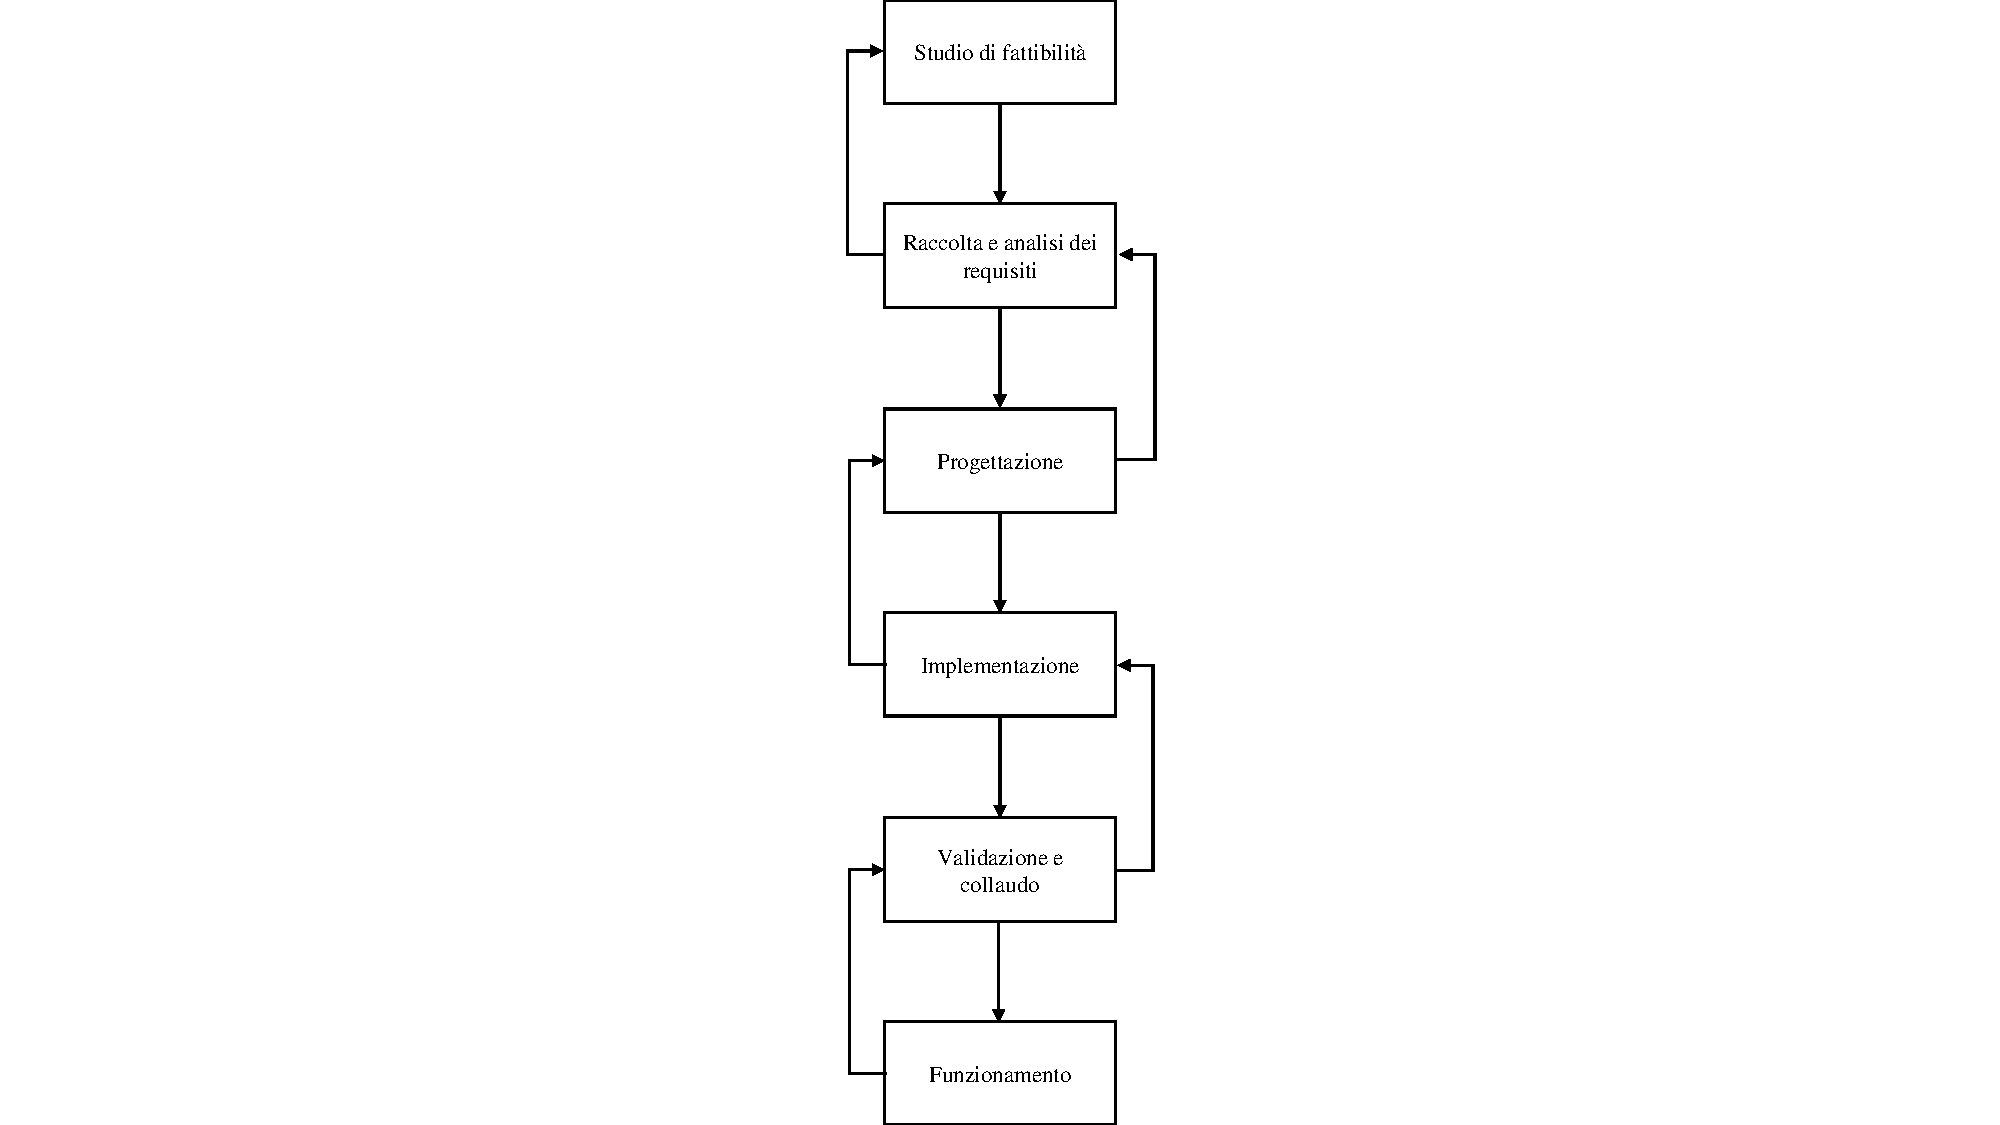
\includegraphics[width=0.4\textwidth]{img/ciclo_di_vita_sis_inf.pdf}
		\caption{Ciclo di vita di un sistema informativo.}
	\end{figure}

	\newpage
	
	
	
	
	\subsection{Metodologie di progettazione e basi di dati}
	
	Una \textbf{metodologia di progettazione} consiste in:
	
	\begin{itemize}
		\item[\ding{51}] \textbf{Decomposizione} dell'intera attività di progetto in passi successivi indipendenti tra loro.
		
		\item[\ding{51}] \textbf{Strategie} da seguire nei vari passi e \textbf{criteri} nel caso di alternative.
		
		\item[\ding{51}] \textbf{Modelli di riferimento} per descrivere i dati in ingresso e uscita delle varie fasi.
	\end{itemize}

	\noindent
	Le \textbf{proprietà} che una metodologia deve garantire sono:
	
	\begin{itemize}
		\item[\ding{72}] \textbf{\emph{Generalità}} rispetto alle applicazioni e ai sistemi in gioco;
		
		\item[\ding{72}] \textbf{\emph{Qualità del prodotto}} in termini di correttezza, completezza ed efficienza rispetto alle risorse impiegate;
		
		\item[\ding{72}] \textbf{\emph{Facilità d'uso}} delle strategie e dei modelli di riferimento.
	\end{itemize}

	%\newpage

	Negli anni si è \emph{consolidata una metodologia} di progetto che ha dato prova di soddisfare pienamente le proprietà descritte. Si basa sull'idea di separare le decisioni relative a \dquotes{cosa} rappresentare in una base di dati (prima fase), da quelle relative a \dquotes{come} farlo (seconda e terza fase):
	
	\begin{itemize}
		\item[\ding{42}] \textbf{Progettazione concettuale.}\newline
		\textcolor{Red3}{\textbf{Obbiettivo:}} rappresentare le specifiche informali della realtà di interesse in termini di una descrizione formale e completa. La \textbf{\underline{rappresentazione}} \textbf{\underline{deve essere indipendente}} dai criteri di rappresentazione utilizzati nei sistemi di gestione di basi di dati.\newline
		\textcolor{Green4}{\textbf{Prodotto di questa fase:}} \underline{schema concettuale}. È un documento formale che rappresenta il contenuto della base di dati in modo indipendente dall'implementazione (DBMS).\newline
		\textcolor{Blue3}{\textbf{Applicazione:}} cercare di rappresentare il \textbf{contenuto informativo} della base di dati, senza preoccuparsi né della modalità con le quali queste informazioni verranno codificate in un sistema reale, né dell'efficienza dei programmi che faranno uso di queste informazioni.\label{progettazione concettuale}
		
		\item[\ding{42}] \textbf{Progettazione logica.}\newline
		\textcolor{Red3}{\textbf{Obbiettivo:}} traduzione dello schema concettuale prodotto nella fase precedente, in termini del modello di rappresentazione dei dati adottato dal sistema di gestione di base di dati a disposizione.\newline
		\textcolor{Green4}{\textbf{Prodotto di questa fase:}} \underline{schema logico}.\newline
		\textcolor{Blue3}{\textbf{Applicazione:}} durante la traduzione, le scelte progettuali si \underline{devono} basare anche su criteri di ottimizzazione delle operazioni da effettuare sui dati.\label{progettazione logica}
		
		\item[\ding{42}] \textbf{Progettazione fisica.}\newline
		\textcolor{Red3}{\textbf{Obbiettivo:}} lo schema logico viene completato con la specifica dei parametri fisici di memorizzazione dei dati.\newline
		\textcolor{Green4}{\textbf{Prodotto di questa fase:}} \underline{schema fisico}.\newline\label{progettazione fisica}
	\end{itemize}

	\newpage
	
	
	
	
	\subsection{Il modello Entità-Relazione (E-R)}\label{Il modello Entità-Relazione (E-R)}
	
	Il \textcolor{Red3}{\textbf{\emph{modello Entità-Relazione}}} è un modello \textbf{concettuale} di dati, quindi utilizzato nella \textbf{progettazione concettuale}, e fornisce una serie di strutture, chiamati \textbf{\emph{costrutti}}, atte a descrivere la realtà di interesse in una maniera facile da comprendere e che prescinde dai criteri di organizzazione dei dati nei calcolatori.
	
	I \underline{costrutti vengono utilizzati} per \textbf{definire schemi} che \textbf{descrivono l'organizzazione e la struttura delle occorrenze} (o \textbf{istanze}) \textbf{dei dati}, ovvero, dei valori assunti dai dati al variare del tempo.
	
	\noindent
	Si possono \underline{riassumere le caratteristiche} del modello Entità-Relazione:
	
	\begin{itemize}
		\item[\ding{42}] \textcolor{SpringGreen4}{\textbf{\emph{Modello concettuale}.}} Utilizzato durante la progettazione concettuale (definizione al paragrafo~\ref{progettazione concettuale}) di una base di dati.
		
		\item[\ding{42}] \textcolor{SpringGreen4}{\textbf{\emph{Strumenti formali}.}} Vengono messi a disposizione diversi strumenti per definire la \textbf{struttura} e le \textbf{proprietà} di una base di dati (\emph{esempio i costrutti}).
		
		\item[\ding{42}] \textcolor{SpringGreen4}{\textbf{\emph{Indipendente dalla tecnologia}.}} Essendo un modello astratto, l'obbiettivo è quello di definire la struttura e le proprietà della base di dati (\underline{non di implementarla!}).
		
		\item[\ding{42}] \textcolor{SpringGreen4}{\textbf{\emph{Formale}.}} È facile da utilizzare nonostante non ammetta ambiguità.
		
		\item[\ding{42}] \textcolor{SpringGreen4}{\textbf{\emph{Grafico}.}} La sintassi è prettamente grafica e questo aumenta anche la leggibilità.
	\end{itemize}

	\newpage
	
	
	
	
	\subsection{I costrutti principali del modello}
	
	Si analizzano i principali costrutti di questo modello: entità (pagina~\pageref{entità}), relazioni(pagina~\pageref{relazioni}) e attributi (pagina~\pageref{attributi}).
	
	\subsubsection{Entità}\label{entità}
	\textcolor{Red3}{\textbf{Definizione.}} Rappresentano \textbf{classi di oggetti} (per esempio, fatti, cose, persone) \textbf{che hanno proprietà comuni ed esistenza \dquotes{autonoma} ai fini dell'applicazione di interesse}. Per esempio, \dquotes{città, dipartimento, impiegato, acquisto e vendita} sono entità di un'applicazione aziendale. Inoltre, \textbf{ogni entità ha un nome identificativo}, il quale deve essere \textbf{univoco}. In sintesi:
	
	\begin{itemize}
		\item Hanno \textbf{proprietà comuni};
		\item Hanno \textbf{esistenza autonoma};
		\item Hanno \textbf{identificazione univoca}.
	\end{itemize}

	\noindent
	\textcolor{Green4}{\textbf{Sintassi grafica.}}
	
	\begin{figure}[!htp]
		\centering
		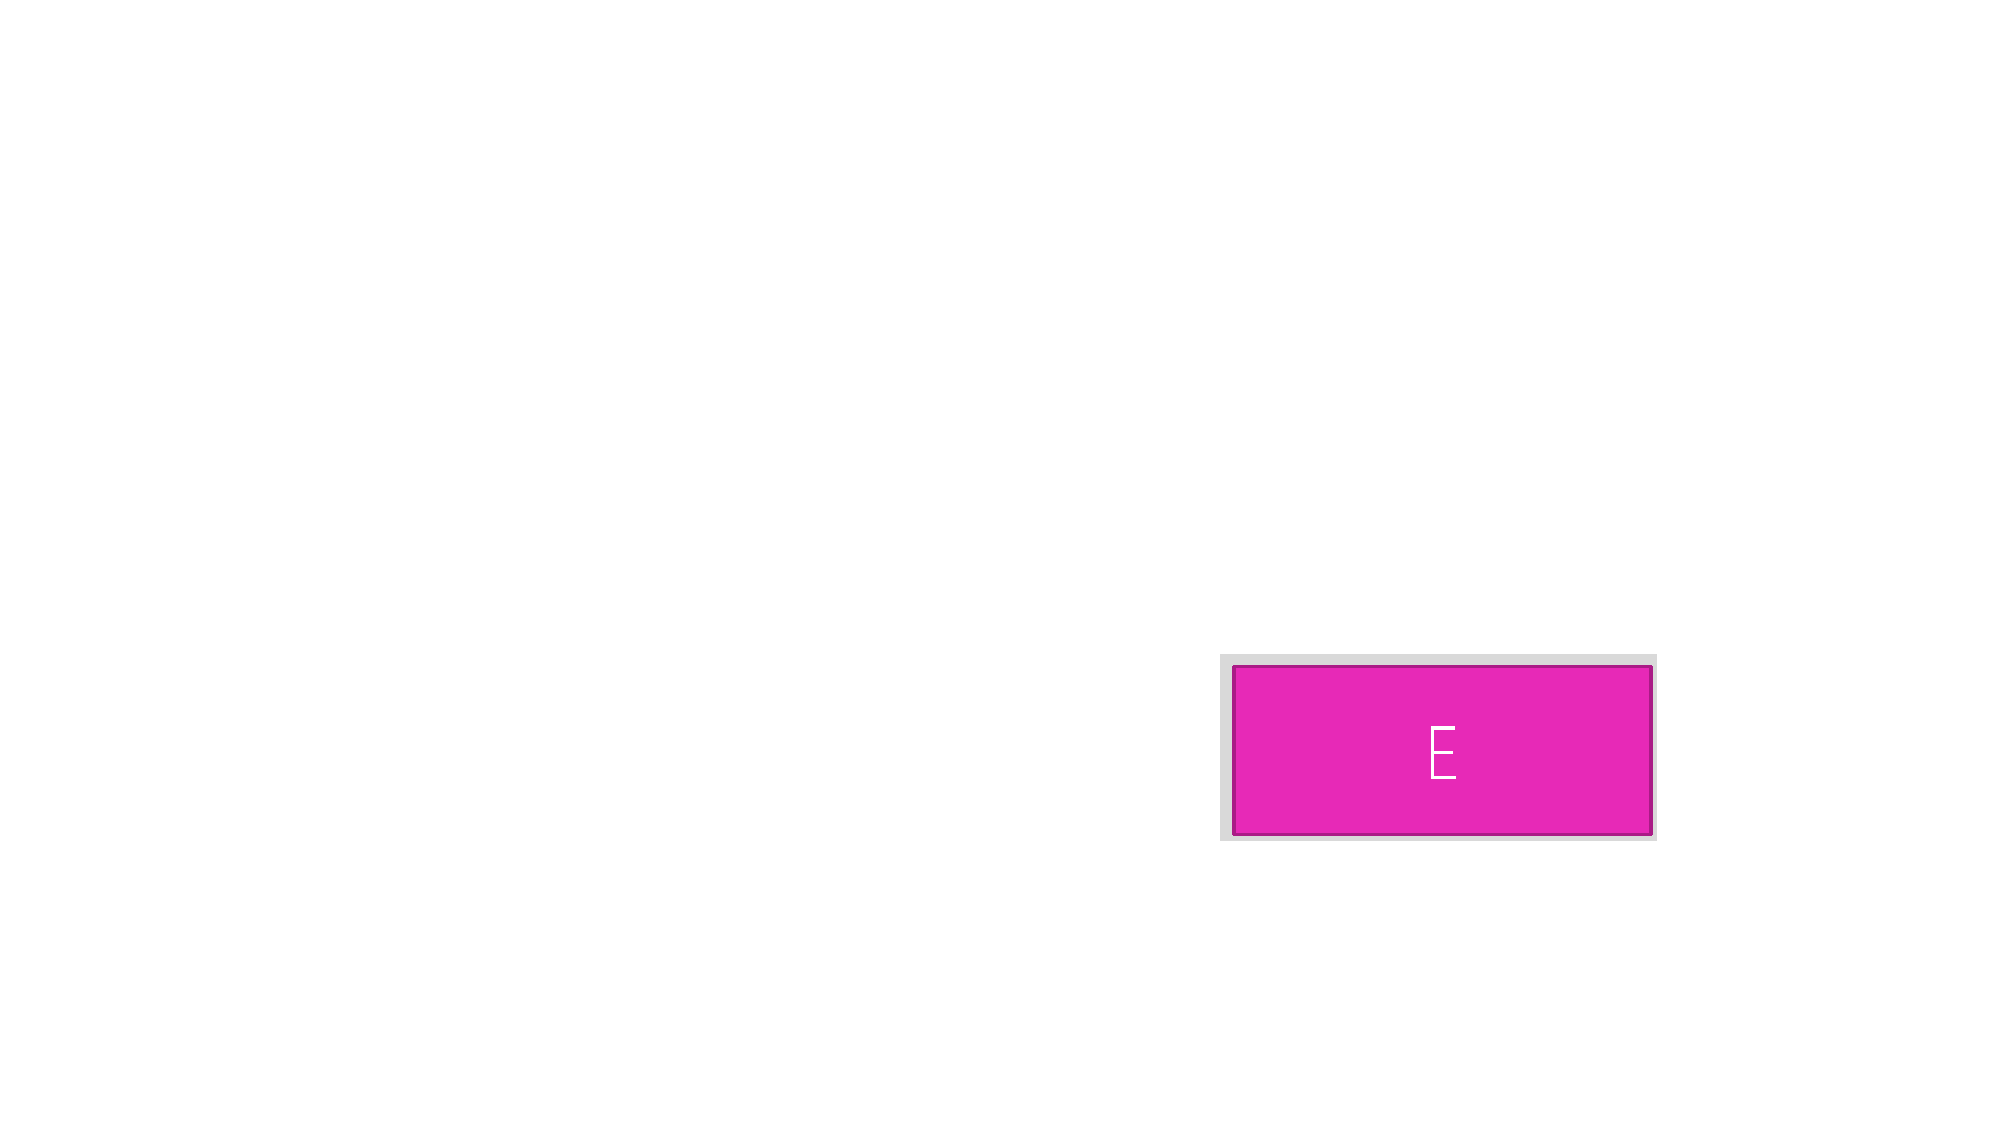
\includegraphics[width=0.5\textwidth]{img/entita_def.pdf}
		\caption{Sintassi grafica dell'entità.}
	\end{figure}

	\noindent
	\textcolor{blue}{\textbf{Istanza (o occorrenza).}} Un'\textbf{istanza} (o occorrenza) di un'entità è un \textbf{oggetto della classe che l'entità rappresenta}. Le città di Roma, Milano e Palermo sono esempi di occorrenze dell'entità \dquotes{Città}.\newline
	\textbf{\underline{Attenzione!}} L'istanza di un'entità \textbf{\emph{non è un valore}} che identifica un oggetto (per esempio, il cognome dell'impiegato o il suo codice fiscale),\textbf{\emph{ ma è l'oggetto stesso}} (l'impiegato in \dquotes{carne e ossa}). Quindi, un'\textbf{istanza ha un'esistenza indipendente dalle proprietà a esso associate}.
	
	Un’istanza dell’entità $E$ è un oggetto appartenente alla classe rappresentata da $E$. Si indica con $I(E)$ l’insieme delle istanze di $E$ che esistono nella base di dati in un certo istante.
	
	\newpage
	
	
	
	
	\subsubsection{Relazioni (o associazioni)}\label{relazioni}
	
	\textcolor{Red3}{\textbf{Definizione.}} Rappresentano \textbf{legami logici}, significativi per l'applicazione di interesse, \textbf{tra due o più entità}. Per esempio, \dquotes{Residenza} è una relazione che sussiste tra le entità \dquotes{Città} e \dquotes{Impiegato}.Nello schema E-R, \textbf{ogni relazione ha un nome identificativo univoco}.
	
	\noindent
	Le relazioni possono essere di \textbf{tipo}:
	
	\begin{itemize}
		\item \textbf{\emph{Ricorsive}}, ovvero \textbf{relazioni tra un'entità e se stessa}. Per esempio, la relazione \dquotes{Collega} sull'entità \dquotes{Impiegato} connette coppie di impiegati che lavorano insieme.
		
		\item \textbf{\emph{n-arie}}, ovvero \textbf{relazioni che coinvolgono più di due entità}. Per esempio, la relazione \dquotes{Fornitura} tre le tre entità \dquotes{Fornitore, Prodotto e Dipartimento} descrive il fatto che un fornitore rifornisce un dipartimento di un certo prodotto.
	\end{itemize}

	\noindent
	\textbf{\underline{Nota fondamentale:}} \textbf{per eseguire una relazione, le entità devono essere tutte piene o con almeno un dato all'interno.} \newline
	
	\noindent
	\textcolor{Green4}{\textbf{Sintassi grafica.}} Una relazione $R$ si rappresenta nello schema con un \textbf{rombo} a cui si collegano attraverso linee spezzate le entità coinvolte nella relazione. Il nome della relazione viene scritto a fianco del rombo.
	
	\begin{figure}[!htp]
		\centering
		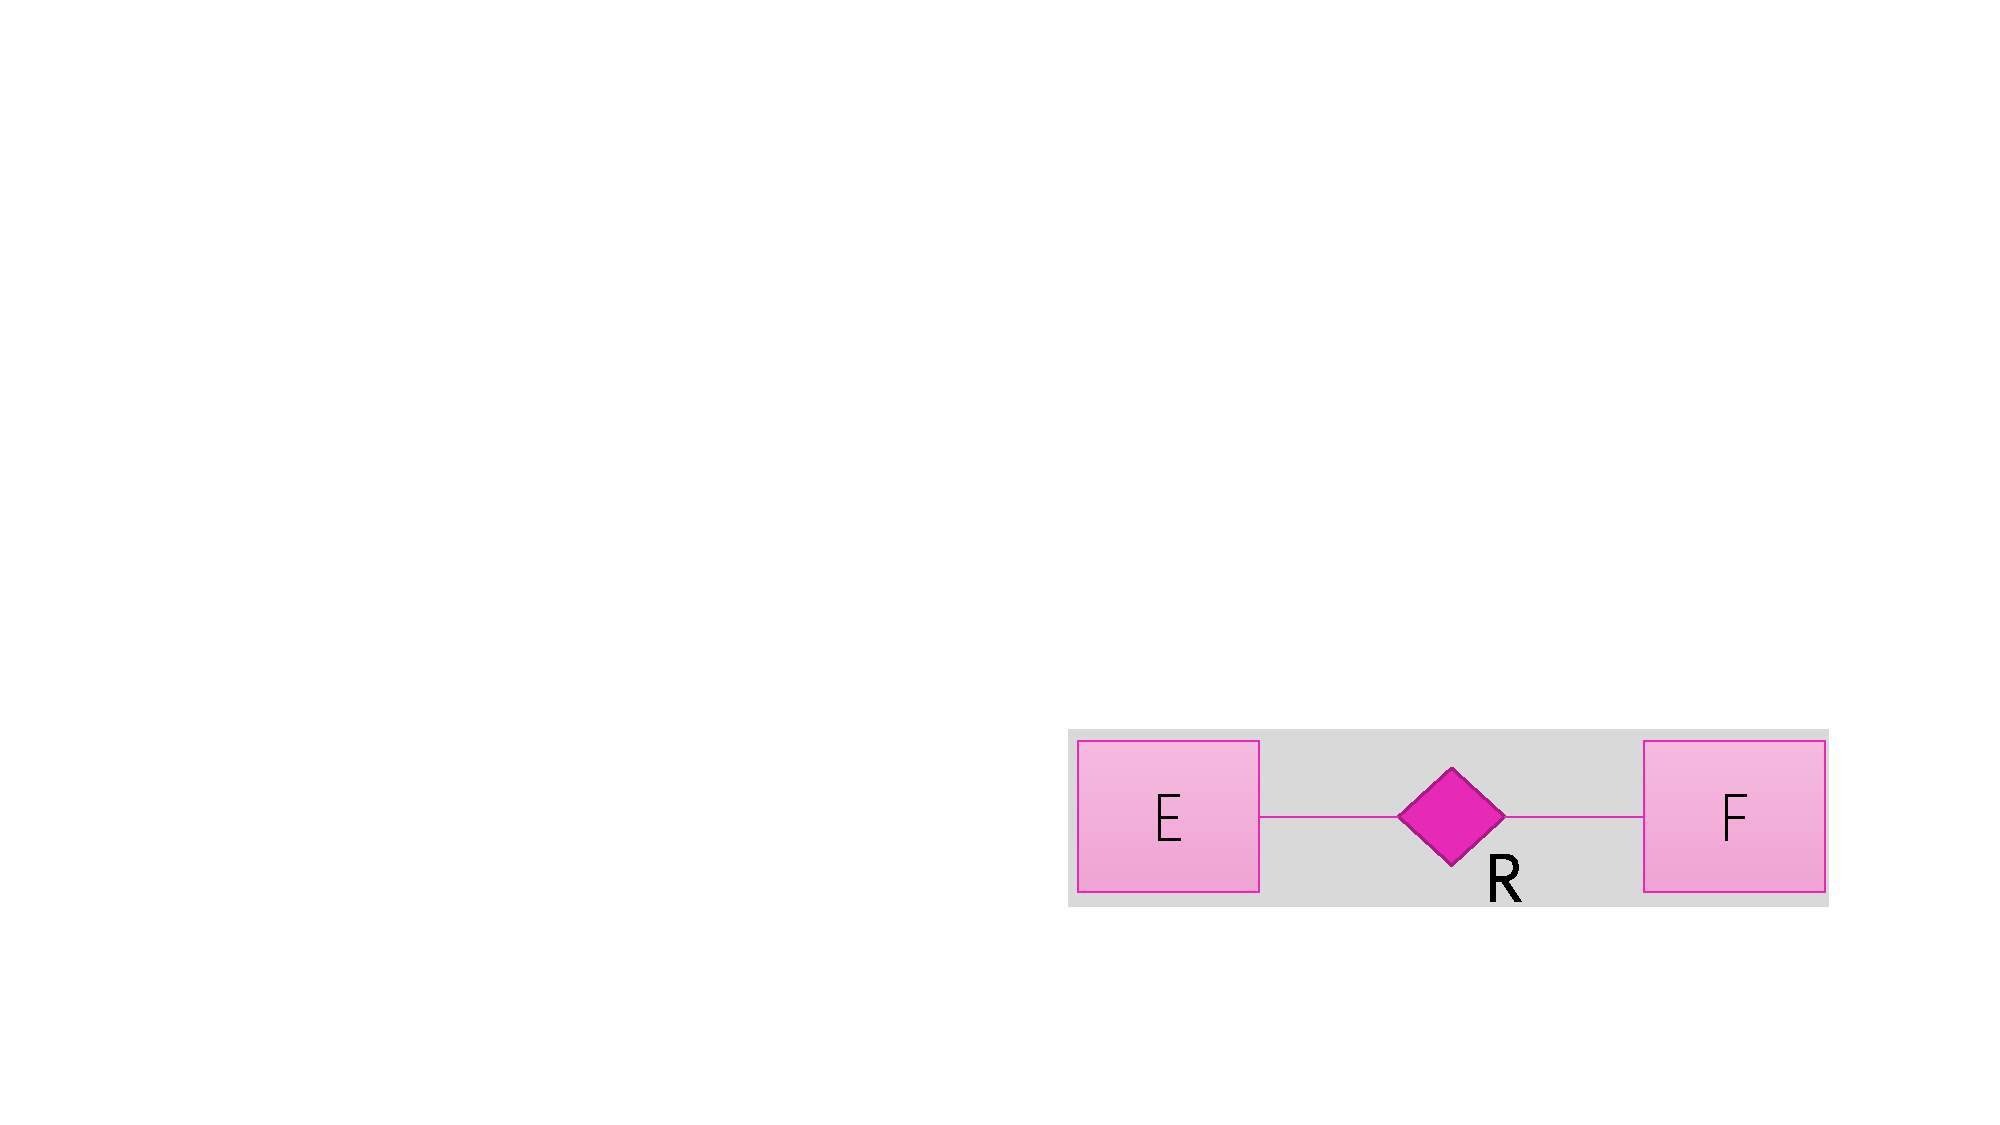
\includegraphics[width=0.6\textwidth]{img/relazione_def.pdf}
		\caption{Sintassi grafica della relazione.}
	\end{figure}

	\noindent
	\textcolor{blue}{\textbf{Istanza (o occorrenza).}} Un'istanza di relazione è un'\textbf{ennupla costituita da istanze di entità, una per ciascuna delle entità coinvolte}.
	
	\noindent
	Data una relazione $R$ tra $n$ entità $E_1, \cdots, E_n$, un’istanza della relazione $R$ è una ennupla di istanze di entità:
	
	\begin{equation*}
		\left(e_1, \cdots, e_n\right) \text{ dove } e_i \in I(E_i), 1\le i \le n
	\end{equation*}

	\noindent
	Infine, esiste una relazione importante. Data una relazione $R$ tra $n$ entità, vale sempre la seguente proprietà sull’insieme delle istanze di $R (I(R))$:
	
	\begin{equation*}
		I(R) \subseteq I(E_1) \times \cdots \times I(E_n)
	\end{equation*}
	
	\newpage
	
	
	
	
	\subsubsection{Attributi}\label{attributi}
	
	\textcolor{Red3}{\textbf{Definizione.}} Descrivono le \textbf{proprietà elementari} di entità o relazioni che sono di interesse ai fini dell'applicazione. Per esempio, \dquotes{Cognome, Stipendio ed Età} sono possibili attributi dell'entità \dquotes{Impiegato}.
	
	Un attributo associa a ciascun istanza di entità (o relazione) \textbf{\underline{uno e un solo}} valore appartenente a un insieme, chiamato \textbf{\emph{dominio}}, che contiene i valori ammissibili per l'attributo. Per esempio, l'attributo \dquotes{Cognome} dell'entità \dquotes{Impiegato} può avere come dominio l'insieme delle stringhe di $20$ caratteri.
	
	L'attributo può essere visto come una \textbf{funzione che ha come dominio le istanze dell'entità} (o relazione) e come \textbf{codominio l'insieme dei valori ammissibili}:
	
	\begin{equation*}
		f_{a} : I\left(E\right) \rightarrow D
	\end{equation*}

	\begin{itemize}
		\item $a$ è un attributo dell'entità $E$;
		
		\item $I\left(E\right)$ è l'insieme delle istanze di $E$;
		
		\item $D$ è l'insieme dei valori ammissibili.
	\end{itemize}
	
	\noindent
	\textcolor{Green4}{\textbf{Sintassi grafica.}}
	
	\begin{figure}[!htp]
		\centering
		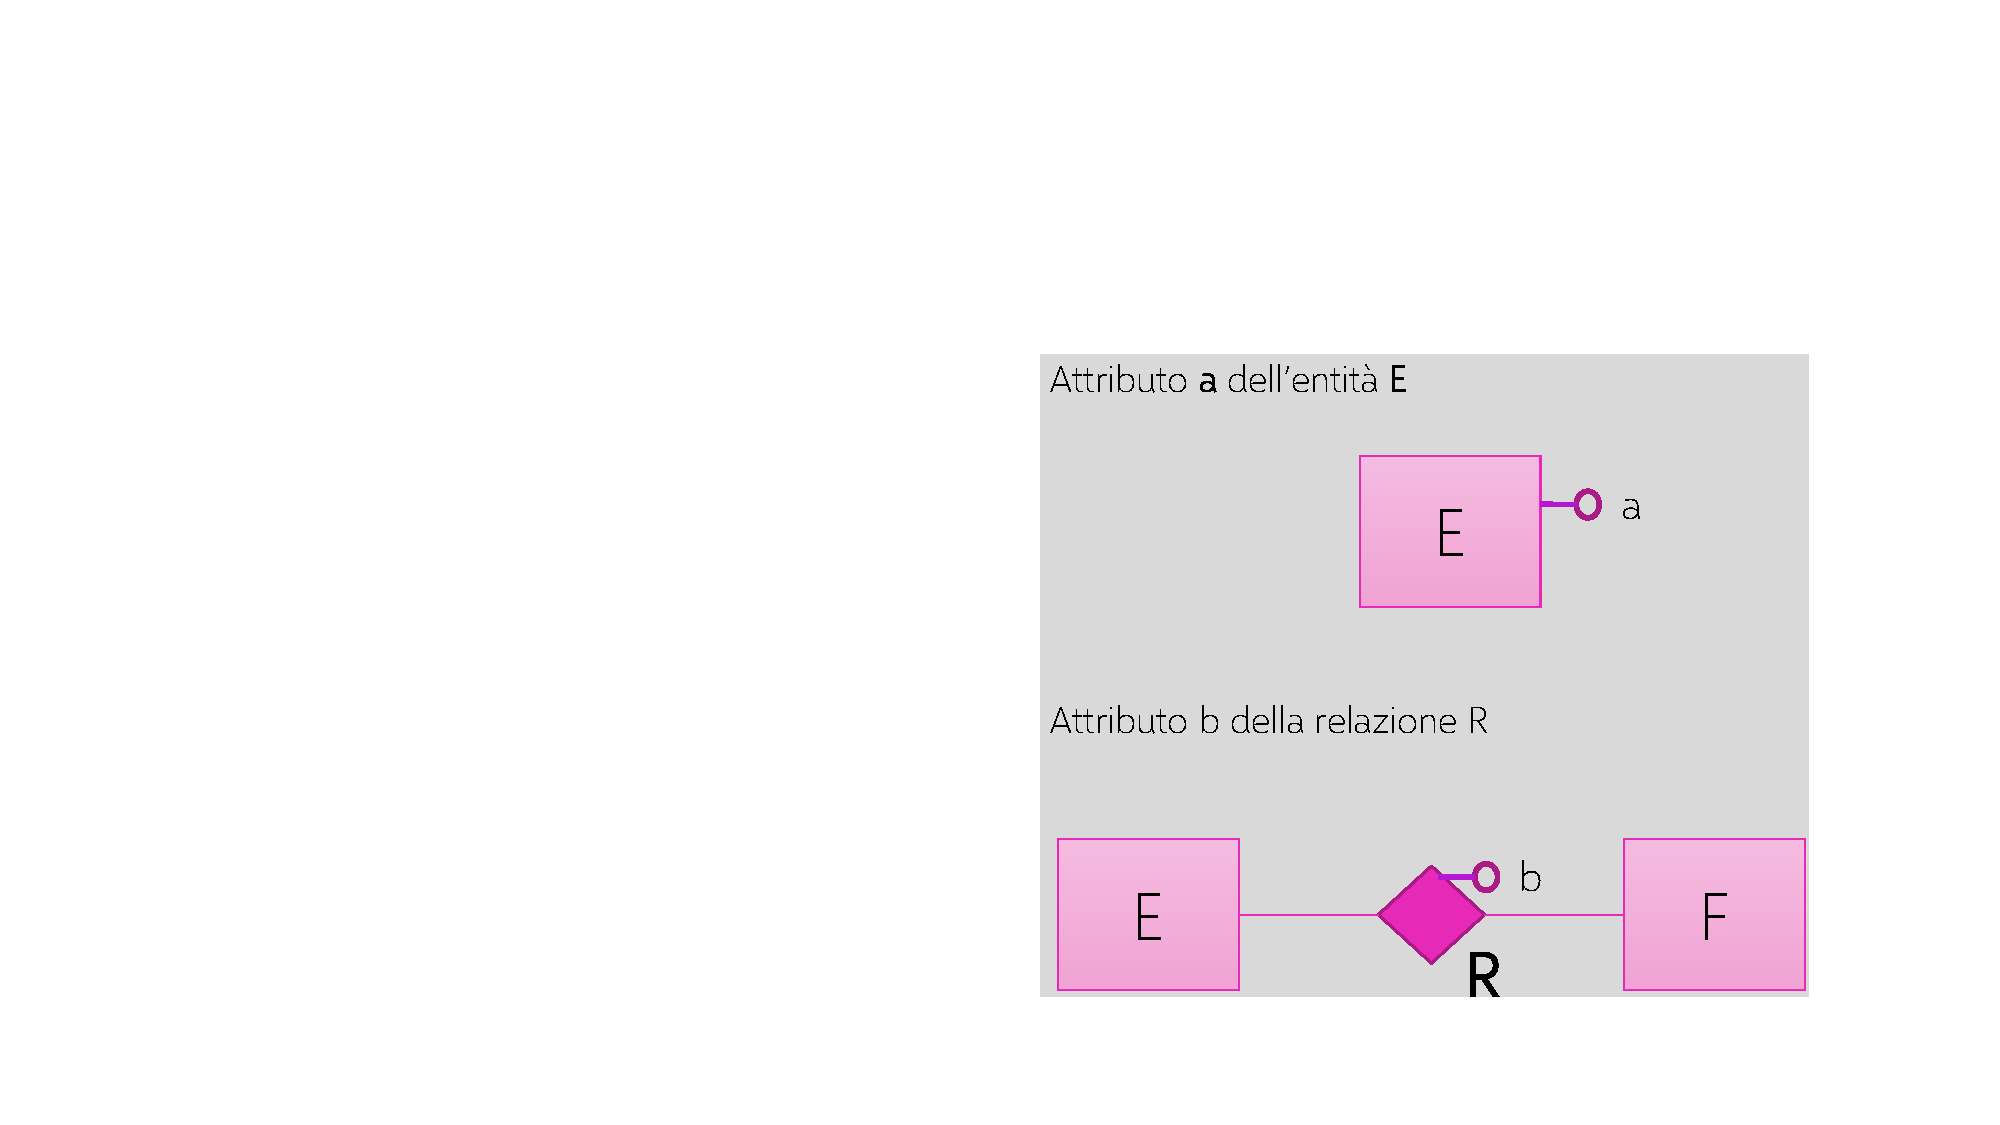
\includegraphics[width=0.5\textwidth]{img/attributo_def.pdf}
		\caption{Sintassi grafica dell'attributo.}
	\end{figure}
	
	\noindent
	\textcolor{blue}{\textbf{Istanza (o occorrenza).}} Dato un attributo $a$ di un'entità $E$ (o relazione $R$), un'istanza di $a$ è il valore $v$ che esso assume su un'istanza di $E$ (o istanza di $R$).
	
	Quindi, data un'istanza $e$ dell'entità $E$ (o relazione $R$), l'istanza di un suo attributo $a$ si ottiene dalla funzione $f_{a}$ applicata a $e$:
	
	\begin{equation*}
		\text{valore di } a \text{ su } e = f_{a}\left(e\right)
	\end{equation*}

	\noindent
	\fbox{%
		\parbox{\textwidth}{%
			\textcolor{Red3}{\textbf{\underline{Attributi composti.}}}\newline
			
			Questo tipo di attributo viene introdotto solo a fini didattici, ma l'obbiettivo è quello di usare unicamente gli attributi normali. Talvolta potrebbe tornare comodo raggruppare \textbf{attributi di una medesima entità o relazione che presentano affinità nel loro significato o uso}: tale insieme prende il nome di \textbf{attributo composto}. Per esempio, gli attributi \dquotes{Via, Numero civico e CAP} dell'entità \dquotes{Persona} per formare l'attributo composto \dquotes{Indirizzo}.
		}%
	}

	\newpage
	
	\subsection{Altri costrutti del modello}
	
	I rimanenti costrutti del modello E-R sono le cardinalità delle relazioni e degli attributi e gli identificatori.
	
	\subsubsection{Cardinalità delle relazioni}
	
	\textcolor{Red3}{\textbf{Definizione.}} Le \textbf{cardinalità} vengono \textbf{specificate per ciascuna entità collegata ad una relazione} e descrivono il \textbf{numero minimo e massimo di occorrenze} di relazione a cui una occorrenza dell'entità può partecipare.
	
	Più formalmente, data una relazione $R$ i vincoli di cardinalità vengono specificati per ogni entità $E_{i}$ coinvolta nella relazione $R$ e specificano: il numero massimo e il numero minimo di istanze di $R$ a cui un'istanza di $E_{i}$ deve/può partecipare.
	
	In parole povere, dicono quante volte, in una relazione tra entità, un'istanza di una di queste entità può essere legata a istanze delle altre entità coinvolte. \textbf{\underline{Per esempio}}, in una relazione \dquotes{Assegnamento} tra le entità \dquotes{Impiegato} e \dquotes{Incarico} si specifica per la prima entità una cardinalità minima pari a uno e una cardinalità massima pari a cinque. Quindi, un impiegato può partecipare a un minimo di una occorrenza e a un massimo di cinque occorrenze della relazione \dquotes{Assegnamento}.\newline
	
	\noindent
	\textbf{\underline{N.B.}} Specificando \textbf{zero come cardinalità minima}, si impone che un'occorrenza può apparire oppure no.\newline
	
	\noindent
	È possibile \textbf{assegnare un qualunque valore intero \underline{non negativo} a una cardinalità di una relazione con l'\underline{unico vincolo} che la cardinalità \emph{minima} deve essere \underline{minore o uguale} della cardinalità \emph{massima}}.
	
	\noindent
	Tuttavia, nella maggior parte dei casi, è sufficiente utilizzare solamente tre simboli: $0$, $1$ e $N$ (molti).
	
	\begin{itemize}[label=\ding{72}]
		\item \textbf{\underline{Cardinalità minima.}}
		\begin{itemize}
			\item \textbf{Zero.} La partecipazione dell'entità relativa è \emph{\textbf{opzionale}};
			\item \textbf{Uno.} La partecipazione dell'entità relativa è \emph{\textbf{obbligatoria}}.
		\end{itemize}
	
		\item \textbf{\underline{Cardinalità massima.}}
		\begin{itemize}
			\item \textbf{Uno.} La partecipazione dell'entità relativa è come una funzione che associa a una occorrenza dell'entità una sola occorrenza (o nessuna) dell'altra entità che partecipa alla relazione;
			\item \textbf{N (molti).} Esiste un'associazione con un numero arbitrario di occorrenze dell'altra entità.
		\end{itemize}
	\end{itemize}

	\noindent
	\textcolor{Green4}{\textbf{Sintassi grafica.}}
	
	\begin{figure}[!htp]
		\centering
		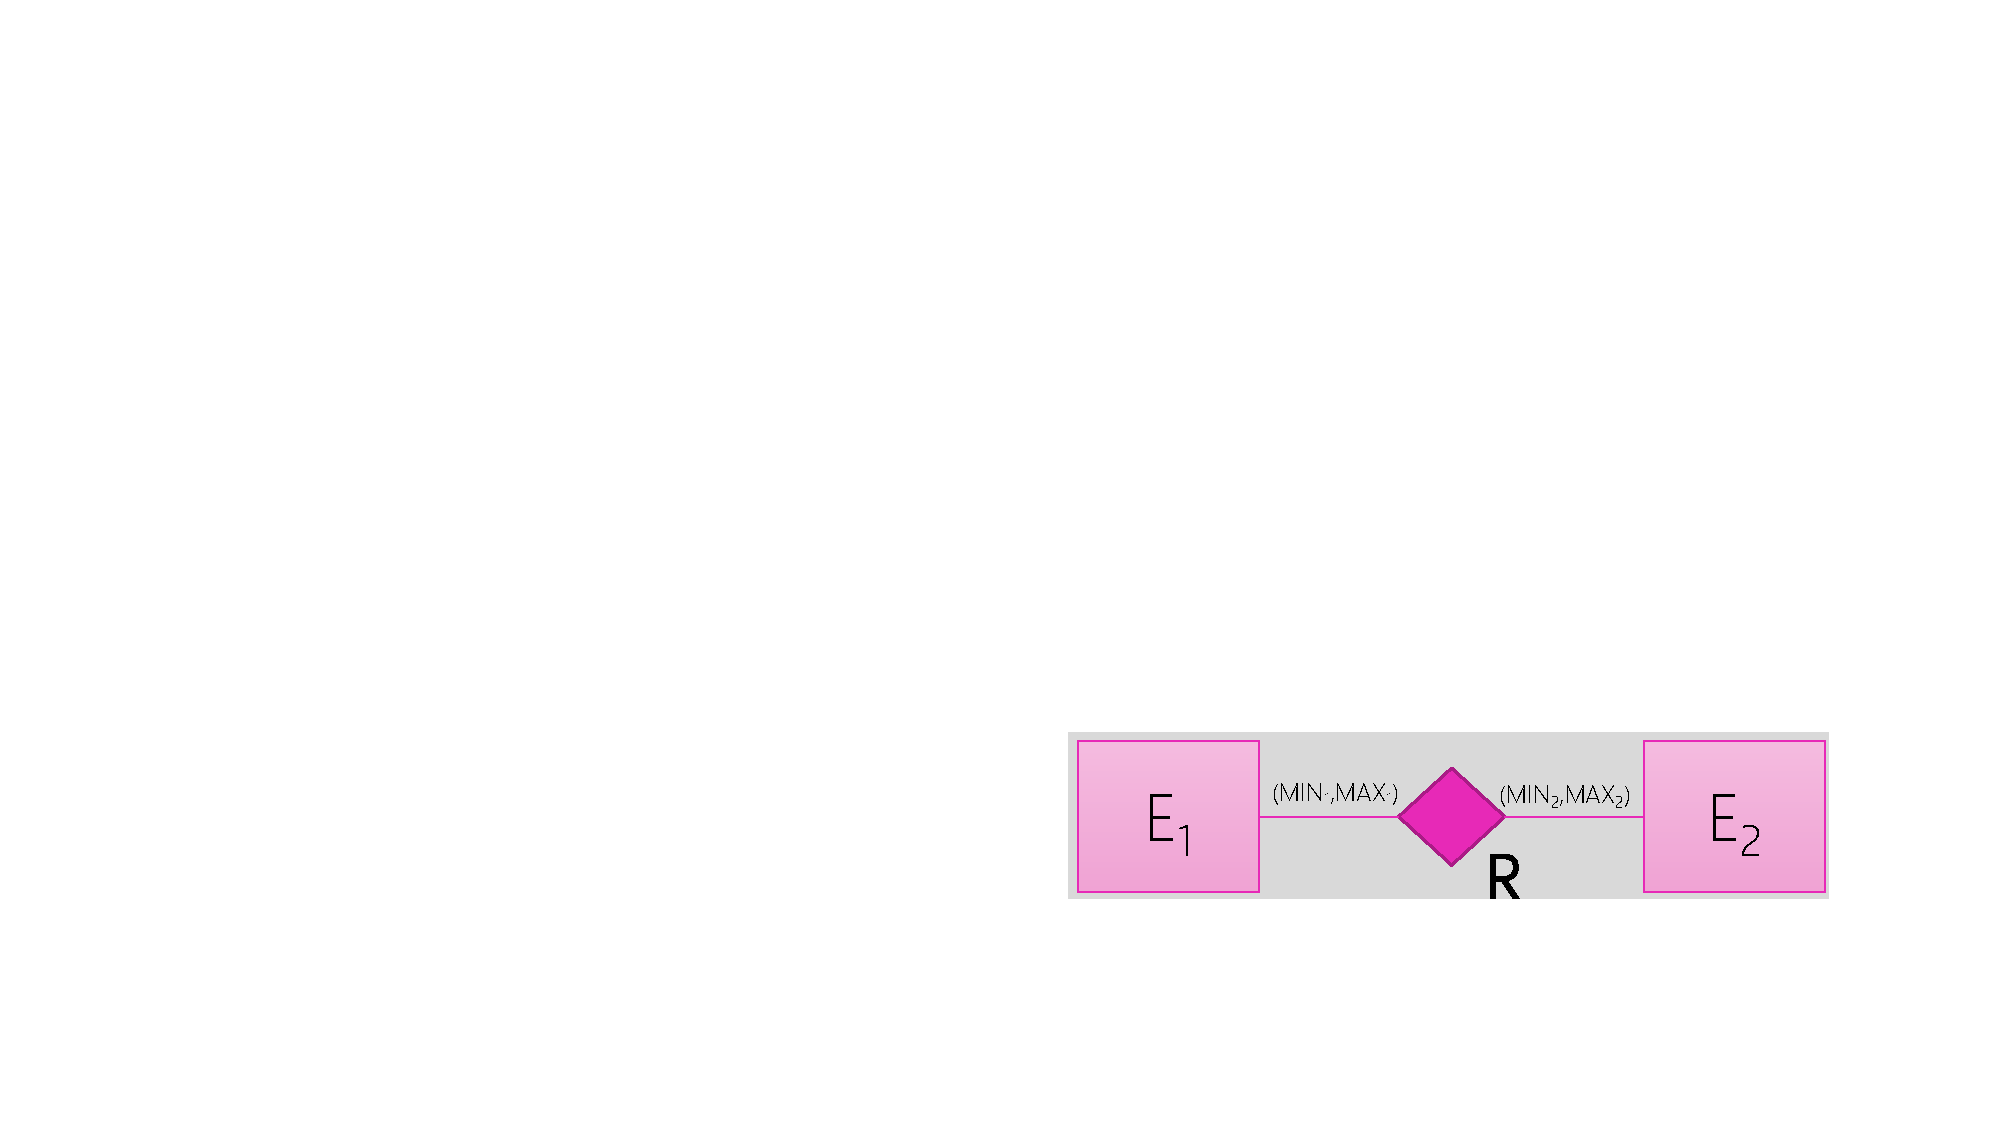
\includegraphics[width=0.52\textwidth]{img/cardinalita_def.pdf}
		\caption{Sintassi grafica della cardinalità.}
	\end{figure}
	
	\newpage

	\subsubsection{Cardinalità degli attributi}
	
	\textcolor{Red3}{\textbf{Definizione.}} Le \textbf{cardinalità degli attributi} è specificata per gli attributi di entità o relazione e hanno l'\textbf{\underline{obbiettivo}} di \textbf{descrivere il numero minimo e massimo di valori dell'attributo associati a ogni occorrenza di entità o relazione}.\newline
	
	\noindent
	Solitamente, il valore di cardinalità pari $\left(1,1\right)$,  ma si possono avere vari casi:
	
	\begin{itemize}
		\item $\left(1, 1\right) \longrightarrow$ L'attributo rappresenta una funzione che associa ad ogni occorrenza di entità un solo valore dell'attributo. Solitamente viene omesso e, come si vede nell'immagine~\ref{esempio cardinalità attributi}, la \dquotes{Persona} ha uno e un solo \dquotes{Cognome};
		
		\item $\left(0, 1\right) \longrightarrow$ L'attributo con cardinalità minima pari a zero vuol dire che è \textbf{opzionale} e la cardinalità massima pari a uno indica che nel \textbf{caso in cui esista}, questo valore è \textbf{unico}. Nell'esempio in figura~\ref{esempio cardinalità attributi}, la persona può avere solo un numero di patente, ma potrebbe anche non avercela;
		
		\item $\left(1, N\right) \longrightarrow$ L'attributo deve esistere, ma contiene più valori, quindi si dice che è \textbf{multivalore};
		
		\item $\left(0, N\right) \longrightarrow$ L'attributo è opzionale, ma se esiste può essere multivalore.
	\end{itemize}
	
	\begin{figure}[!htp]
		\centering
		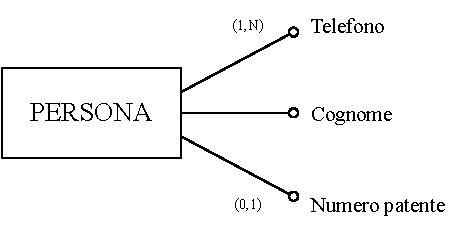
\includegraphics[width=0.5\textwidth]{img/cardinalita-attributi_def.pdf}
		\caption{Esempio di cardinalità degli attributi.}\label{esempio cardinalità attributi}
	\end{figure}

	\newpage

	\subsubsection{Identificatori}
	
	\textcolor{Red3}{\textbf{Definizione.}} Vengono \textbf{specificati per ciascuna entità} di uno schema e \textbf{descrivono i} concetti (\textbf{attributi e/o entità}) dello schema che \textbf{permettono di identificare in maniera \underline{univoca} le occorrenze delle entità}.\newline
	
	\noindent
	È assolutamente \textbf{vietato inserire uno o più identificatori all'interno di una relazione}. Quindi, quest'ultima non può avere identificatori interni!\newline
	
	\noindent
	\textbf{Per esempio}, un identificato interno per l'entità \dquotes{Automobile} con attributi \dquotes{Modello, Targa e Colore} è l'attributo \dquotes{Targa}, in quanto non possono esistere due automobili con la stessa targa e quindi due occorrenze dell'entità \dquotes{Automobile} con gli stessi valori sull'attributo \dquotes{Targa}.\newline
	
	\noindent
	Un'entità $E$ può essere identificata da altre entità solo se tali entità sono coinvolte in una relazione a cui $E$ partecipa con cardinalità $\left(1, 1\right)$. Nei casi in cui l'identificazione di un'entità è ottenuta utilizzando altre entità si parla di \textbf{identificatore \underline{esterno}}. \newline
	Per comprendere meglio si espone un \textbf{esempio}. Per identificare univocamente uno studente serve, oltre al numero di matricola, anche la relativa università. Quindi, un identificatore corretto per l'entità \dquotes{Studente} in questo schema è costituito dall'attributo \dquotes{Matricola} e dall'entità \dquotes{Università}.\newline
	
	\noindent
	Quindi, in generale:
	
	\begin{itemize}
		\item Un identificatore può \textbf{coinvolgere uno o più attributi}, ognuno dei quali deve avere cardinalità $\left(1,1\right)$;
		
		\item Un identificatore esterno può \textbf{coinvolgere una o più entità}, ognuna delle quali deve essere membro di una relazione alla quale l'entità da identificare partecipa con cardinalità $\left(1,1\right)$;
		
		\item Un identificatore esterno può \textbf{coinvolgere un'entità che è a sua volta identificata esternamente}, purché non vengano generati, in questa maniera, cicli di identificazione esterna;
		
		\item Ogni \textbf{entità deve avere almeno un identificatore} (interno o esterno), ma ne può avere in generale più di uno.
	\end{itemize}

	\newpage

	\noindent
	\textcolor{Green4}{\textbf{Sintassi grafica.}}
	
	\begin{figure}[!htp]
		\centering
		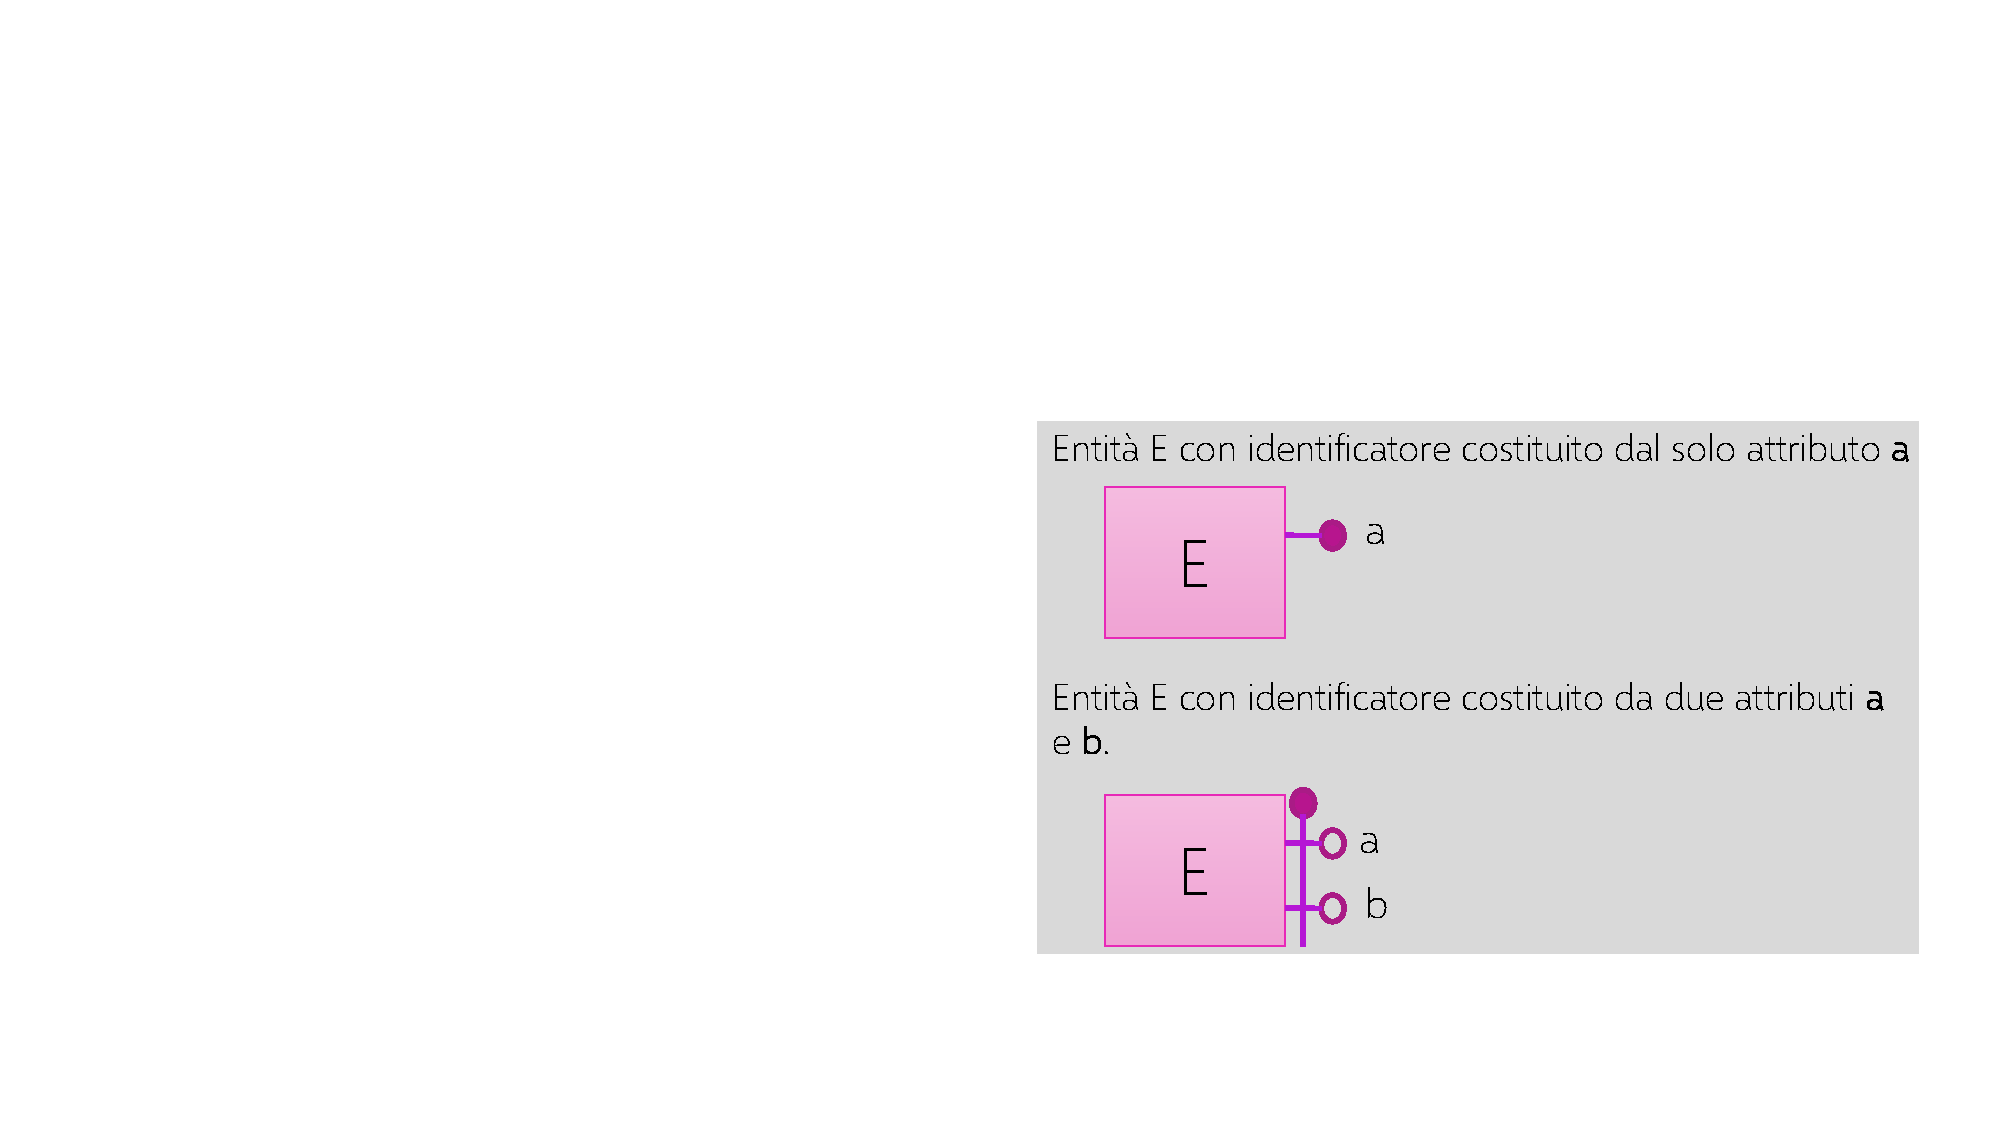
\includegraphics[width=0.7\textwidth]{img/identificatore_def.pdf}
		\caption{Sintassi grafica dell'identificatore.}
	\end{figure}

	\newpage
	
	\subsubsection{Generalizzazioni}
	
	\textcolor{Red3}{\textbf{Definizione.}} Sono i legami logici tra un'entità $E$, chiamata \textbf{entità \underline{genitore}}, e una o più entità $E_{1}, ..., E_{n}$, dette \textbf{entità \underline{figlie}}, di cui $E$ è più generale, nel senso che le comprende come caso particolare. Quindi, si dice che $E$ è \textbf{\underline{generalizzazione}} di $E_{1}, ..., E_{n}$ e che le entità $E_{1}, ..., E_{n}$ sono \textbf{\underline{specializzazioni}} dell'entità $E$.
	
	\textbf{Per esempio}, l'entità \dquotes{Persona} è una generalizzazione delle entità \dquotes{Uomo e Donna}. Invece, \dquotes{Professionista} è una generalizzazione delle entità \dquotes{Ingegnere, Medico e Avvocato}.\newline
	
	\noindent
	\textbf{\underline{Proprietà.}}
	
	\begin{itemize}
		\item \textbf{Ogni occorrenza di un'entità figlia è anche un'occorrenza dell'entità genitore}. Per esempio, una occorrenza dell'entità \dquotes{Avvocato} è anche una occorrenza dell'entità \dquotes{Professionista}.
		
		\item \textbf{Ogni proprietà dell'entità genitore} (come attributi, identificatori, relazioni e altre generalizzazioni) \textbf{è anche una proprietà delle entità figlie}. Per esempio, se l'entità \dquotes{Persona} ha attributi \dquotes{Cognome ed Età}, anche le entità \dquotes{Uomo} e \dquotes{Donna} possiedono questi attributi.
	\end{itemize}

	\noindent
	\textbf{\underline{Classificazioni.}} Le generalizzazioni possono essere classificate:
	
	\begin{itemize}
		\item \textbf{\underline{Totale.}} Ogni occorrenza dell'entità genitore è una occorrenza di almeno una dell'entità figlie. Se non è così, la generalizzazione è \textbf{\underline{parziale}};
		
		\item \textbf{\underline{Esclusiva.}} Ogni occorrenza dell'entità genitore è al massimo un'occorrenza di una delle entità figlie. Se non è così, la generalizzazione è \textbf{\underline{sovrapposta}}.
	\end{itemize}

	\noindent
	In generale, una stessa entità può essere coinvolta in più generalizzazioni diverse. Possono esserci \textbf{generalizzazioni su più livelli}: in questo caso si parla di \textbf{\underline{gerarchia}} di generalizzazioni. Infine, una \textbf{generalizzazione può avere una sola entità figlia}: in questo caso si parla di \textbf{\underline{sottoinsieme}}.
	
	\newpage
	
	\noindent
	\textcolor{Green4}{\textbf{Sintassi grafica.}} Non è difficile da comprendere, ma si presti attenzione a $\left(x, y\right)$. Esse indicano il \textbf{tipo di generalizzazione}:
	
	\begin{itemize}
		\item $\left[t,e\right] \rightarrow$ totale ed esclusiva;
		
		\item $\left[t,s\right] \rightarrow$ totale e sovrapposta;
		
		\item $\left[p,e\right] \rightarrow$ parziale ed esclusiva;
		
		\item $\left[p,s\right] \rightarrow$ parziale e sovrapposta.
	\end{itemize}

	\begin{figure}[!htp]
		\centering
		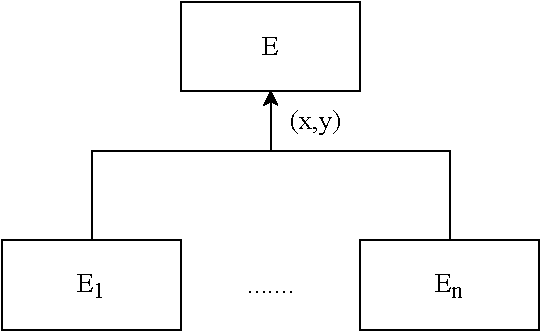
\includegraphics[width=0.6\textwidth]{img/generalizzazione_sintassi.pdf}
		\caption{Sintassi grafica della generalizzazione.}
	\end{figure}

	\newpage
	
	\section{Progettazione concettuale}
	
	\subsection{Strategie di progetto}
	
	Lo sviluppo di uno schema concettuale a partire dalle sue specifiche può essere considerato un processo di ingegnerizzazione.
	
	\subsubsection{Strategia top-down}
	
	Lo schema concettuale viene prodotto mediante una serie di raffinamenti successivi a partire da uno schema iniziale che descrive tutte le specifiche con pochi concetti molto astratti. Lo schema viene poi via via raffinato mediante opportune trasformazioni che aumentano il dettaglio dei vari concetti presenti.\newline
	
	\noindent
	In sintesi:
	
	\begin{enumerate}
		\item \textbf{Fase 1}, si considerano le \emph{specifiche globalmente} e si produce uno schema iniziale completo ma con \emph{pochi concetti} molto \emph{astratti};
		
		\item \textbf{Fase 2}, si esegue un \emph{raffinamento} dei concetti astratti fino ad arrivare allo schema concettuale \emph{completo} in ogni \emph{dettaglio}.
	\end{enumerate}

	\noindent
	\textcolor{Green4}{\textbf{\emph{Vantaggio:}}} il progettista può \textbf{descrivere inizialmente tutte le specifiche dei dati trascurandone i dettagli}, per \textbf{poi entrare nel merito} di un concetto alla volta.\newline
	
	\noindent
	\textcolor{Red3}{\textbf{\emph{Svantaggio:}}} si deve \textbf{possedere} una \textbf{visione globale e astratta} di \emph{tutte} le componenti del sistema, ma solitamente è difficile.
	
	\newpage
	
	\subsubsection{Strategia bottom-up}
	
	Le specifiche iniziali sono suddivise in componenti via via sempre più piccole, fino a quando queste componenti descrivono un frammento elementare della realtà di interesse. A questo punto, le varie componenti vengono rappresentate da semplici schemi concettuali che possono consistere anche in singoli concetti. I vari schemi così ottenuti vengono poi fusi fino a giungere attraverso una completa integrazione di tutte le componenti, allo schema concettuale finale.
	
	La \textbf{differenza rispetto alla strategia top-down} è che i vari concetti presenti nello schema finale vengono via via introdotti durante le varie fasi.\newline
	
	\noindent
	In sintesi:
	
	\begin{enumerate}
		\item \textbf{Fase 1}, si \emph{decompongono} le specifiche iniziali in \emph{parti elementari}, ovvero in frasi che descrivono lo stesso concetto;
		
		\item \textbf{Fase 2}, si \emph{generano} gli schemi per tutte le parti elementari individuate;
		
		\item \textbf{Fase 3}, si \emph{fondono} gli schemi (introducendo altri costrutti del modello E-R) in modo da \emph{integrare} tutti gli schemi componenti e generare lo \emph{schema finale}.
	\end{enumerate}

	\noindent
	\textcolor{Green4}{\textbf{\emph{Vantaggio:}}} questa strategia si adatta a una \textbf{decomposizione del problema in componenti più semplici}, facilmente individuabili, il cui progetto può essere affrontato anche da progettisti diversi.\newline
	
	\noindent
	\textcolor{Red3}{\textbf{\emph{Svantaggio:}}} vengono richieste delle operazioni di \textbf{integrazione di schemi concettuali diversi} che, nel caso di schemi complessi, presentano \textbf{quasi sempre grosse difficoltà}.
	
	\newpage
	
	\subsubsection{Strategia inside-out}
	
	Si individuano inizialmente solo alcuni concetti importanti e poi si procede, a partire da questi, a \dquotes{macchia d'olio}. Si rappresentano cioè prima i concetti in relazione con i concetti iniziali, per poi muoversi verso quelli più lontani attraverso una \dquotes{navigazione} tra le specifiche.\newline
	
	\noindent
	In sintesi:
	
	\begin{enumerate}
		\item \textbf{Fase 1}, si \emph{individua} nelle specifiche alcuni \emph{concetti importanti}, chiamati concetti guida;
		
		\item \textbf{Fase 2}, si \emph{generano} gli schemi per i concetti guida;
		
		\item \textbf{Fase 3}, si \emph{fondono} gli schemi precedenti e si genera lo \emph{schema finale}.
	\end{enumerate}
	
	\noindent
	\textcolor{Green4}{\textbf{\emph{Vantaggio:}}} \textbf{non sono richiesti passi di integrazione}.\newline
	
	\noindent
	\textcolor{Red3}{\textbf{\emph{Svantaggio:}}} è necessario, di volta in volta, \textbf{esaminare tutte le specifiche} per \textbf{individuare concetti non ancora rappresentati} e \textbf{descrivere i nuovi concetti nel dettaglio}.
	
	\newpage
	
	\subsection{Qualità di uno schema concettuale}
	
	L'analisi della qualità dello schema concettuale prodotto può essere suddivisa in diverse fasi:
	
	\begin{itemize}
		\item Correttezza
		\item Completezza
		\item Leggibilità
		\item Minimalità
	\end{itemize}

	\subsubsection{Correttezza}\label{correttezza}

	\textcolor{Red3}{\textbf{\emph{Definizione.}}} Uno schema concettuale è \textbf{corretto} quando \textbf{utilizza propriamente i costrutti} messi a disposizione dal modello concettuale di riferimento.\newline
	
	\noindent
	Gli errori che si possono commettere nello schema concettuale sono principalmente due:
	
	\begin{itemize}
		\item \textcolor{Red3}{\textbf{\emph{Sintattici}}}. Vengono utilizzati costrutti non ammessi. \textcolor{Green4}{Per esempio}, una generalizzazione tra relazioni invece che tra entità.
		
		\item \textcolor{Red3}{\textbf{\emph{Semantici}}}. Vengono usati costrutti senza rispettare la loro definizione. \textcolor{Green4}{Per esempio}, l'uso di una relazione per descrivere il fatto che una entità è specializzazione di un'altra.
	\end{itemize}
	
	\subsubsection{Completezza}\label{completezza}
	
	\textcolor{Red3}{\textbf{\emph{Definizione.}}} Uno schema concettuale è \textbf{completo} quando \textbf{rappresenta tutti i dati} di interesse e quando \textbf{tutte le operazioni possono essere eseguite} a partire dai concetti descritti nello schema.\newline
	
	\noindent
	La completezza è \textbf{possibile verificarla} controllando che tutte le specifiche sui dati siano rappresentate da qualche concetto presente nello schema che stiamo costruendo, e che tutti i concetti coinvolti in un'operazione presente nelle specifiche siano raggiungibili \dquotes{navigando} attraverso lo schema.
	
	\subsubsection{Leggibilità}\label{leggibilità}
	
	\textcolor{Red3}{\textbf{\emph{Definizione.}}} Uno schema concettuale è \textbf{leggibile} quando rappresenta i requisiti in maniera naturale e facilmente comprensibile.\newline
	
	\noindent
	Per garantire questa proprietà è necessario rendere lo schema autoesplicativo, \textcolor{Green4}{per esempio}, mediante una scelta opportuna dei nomi da dare ai concetti. La leggibilità dipende anche da criteri puramente estetici.
	
	\subsubsection{Minimalità}\label{minimalità}
	
	\textcolor{Red3}{\textbf{\emph{Definizione.}}} Uno schema concettuale è \textbf{minimale} quando tutte le specifiche sui dati sono rappresentate una sola volta nello schema.\newline
	
	\noindent
	Uno schema quindi non è minimale quando esistono delle \textbf{ridondanze}, ovvero concetti che possono essere derivati da altri. La minimalità di uno schema si può \textbf{verificare} per ispezione, controllando se esistono concetti che possono essere eliminati dallo schema che stiamo costruendo senza inficiare la sua completezza.
	
	\newpage
	
	\section{Progettazione logica}
	
	\subsection{Fasi della progettazione logica}
	
	L'\textcolor{Red3}{\textbf{obbiettivo}} della progettazione logica è \textbf{produrre uno schema logico che descriva in modo \underline{corretto} ed \underline{efficace} tutte le informazioni contenute nello schema concettuale}.
	
	Le attività principali della progettazione logica sono la riorganizzazione dello schema concettuale e la traduzione in un modello logico:
	
	\begin{itemize}
		\item \textcolor{Red3}{\textbf{\emph{Ristrutturazione dello schema Entità-Relazione}}}: è una fase indipendente dal modello logico scelto e si basa su \textbf{criteri di ottimizzazione} dello schema e di \textbf{semplificazione} della fase successiva. In particolare, le fasi sono:
		\begin{itemize}
			\item Analisi delle ridondanze dovute alla presenza di dati derivabili;
			\item Eliminazione delle generalizzazioni;
			\item Accorpamento/partizionamento di entità e relazioni;
			\item Scelta degli identificatori principali.
		\end{itemize}
	
		\item \textcolor{Red3}{\textbf{\emph{Traduzione verso il modello logico}}}: fa riferimento a uno specifico modello logico (nel nostro caso modello relazionale) e può includere una ulteriore ottimizzazione che si basa sulle caratteristiche del modello logico stesso.
	\end{itemize}
	
	\newpage
	
	\subsection{Traduzione verso il modello logico}
	
	La seconda fase della progettazione logica corrisponde ad una traduzione tra modelli di dati diversi. Si parte da uno schema E-R ristrutturato e si costruisce uno schema logico equivalente, in grado cioè di rappresentare le medesime informazioni.
	
	Si affronta il problema della traduzione caso per caso, iniziando dal caso più generale che ci suggerisce l'idea generale su cui si basa la metodologia di traduzione.
	
	\subsubsection{Entità e attributo opzionale}
	
	L'\textcolor{Red3}{\textbf{\underline{entità}}} si rappresenta una relazione (lettera maiuscola) con lo stesso nome avente per attributi (lettere tra parentesi) i medesimi attributi dell'entità e per chiave il suo identificatore.
	
	\begin{figure}[!htp]
		\centering
		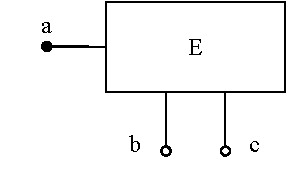
\includegraphics[width=0.4\textwidth]{img/relazionale_entita.pdf}
		\caption{Modello E-R di un'entità.}
	\end{figure}

	\noindent
	Relativo modello relazionale:
	
	\begin{equation*}
		\textbf{E}\left(a,b,c\right)
	\end{equation*}

	\noindent
	Invece, un possibile \textcolor{Red3}{\textbf{\underline{attributo nullo}}} si rappresenta inserendo un asterisco.
	
	\begin{figure}[!htp]
		\centering
		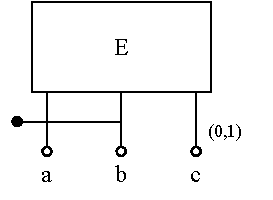
\includegraphics[width=0.4\textwidth]{img/relazionale_attributo_nullo.pdf}
		\caption{Modello E-R di un possibile attributo nullo.}
	\end{figure}
	
	\noindent
	Relativo modello relazionale:
	
	\begin{equation*}
		\textbf{E}\left(\underline{a,b},c^{*}\right)
	\end{equation*}

	\newpage
	
	\subsubsection{Relazione uno a molti}
	
	La \textcolor{Red3}{\textbf{\underline{relazione uno a molti}}} è caratterizzata dal fatto che un'entità è in relazione con un'altra con cardinalità $\left(1,1\right)$ e la corrispondente entità ha cardinalità $\left(x,N\right)$ ($x$ può essere qualsiasi valore minimo).
	
	\begin{figure}[!htp]
		\centering
		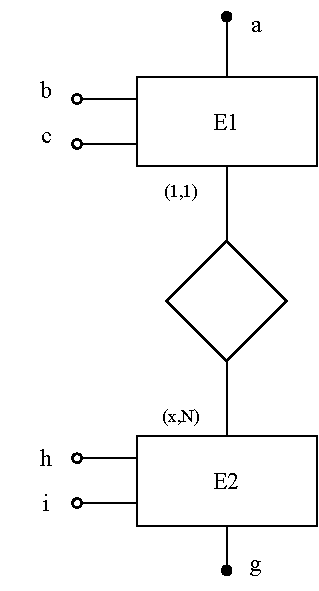
\includegraphics[width=0.5\textwidth]{img/relazionale_uno_a_molti.pdf}
		\caption{Modello E-R di una relazione uno a molti.}
	\end{figure}
	
	\noindent
	Relativo modello relazionale:
	
	\begin{figure}[!htp]
		\centering
		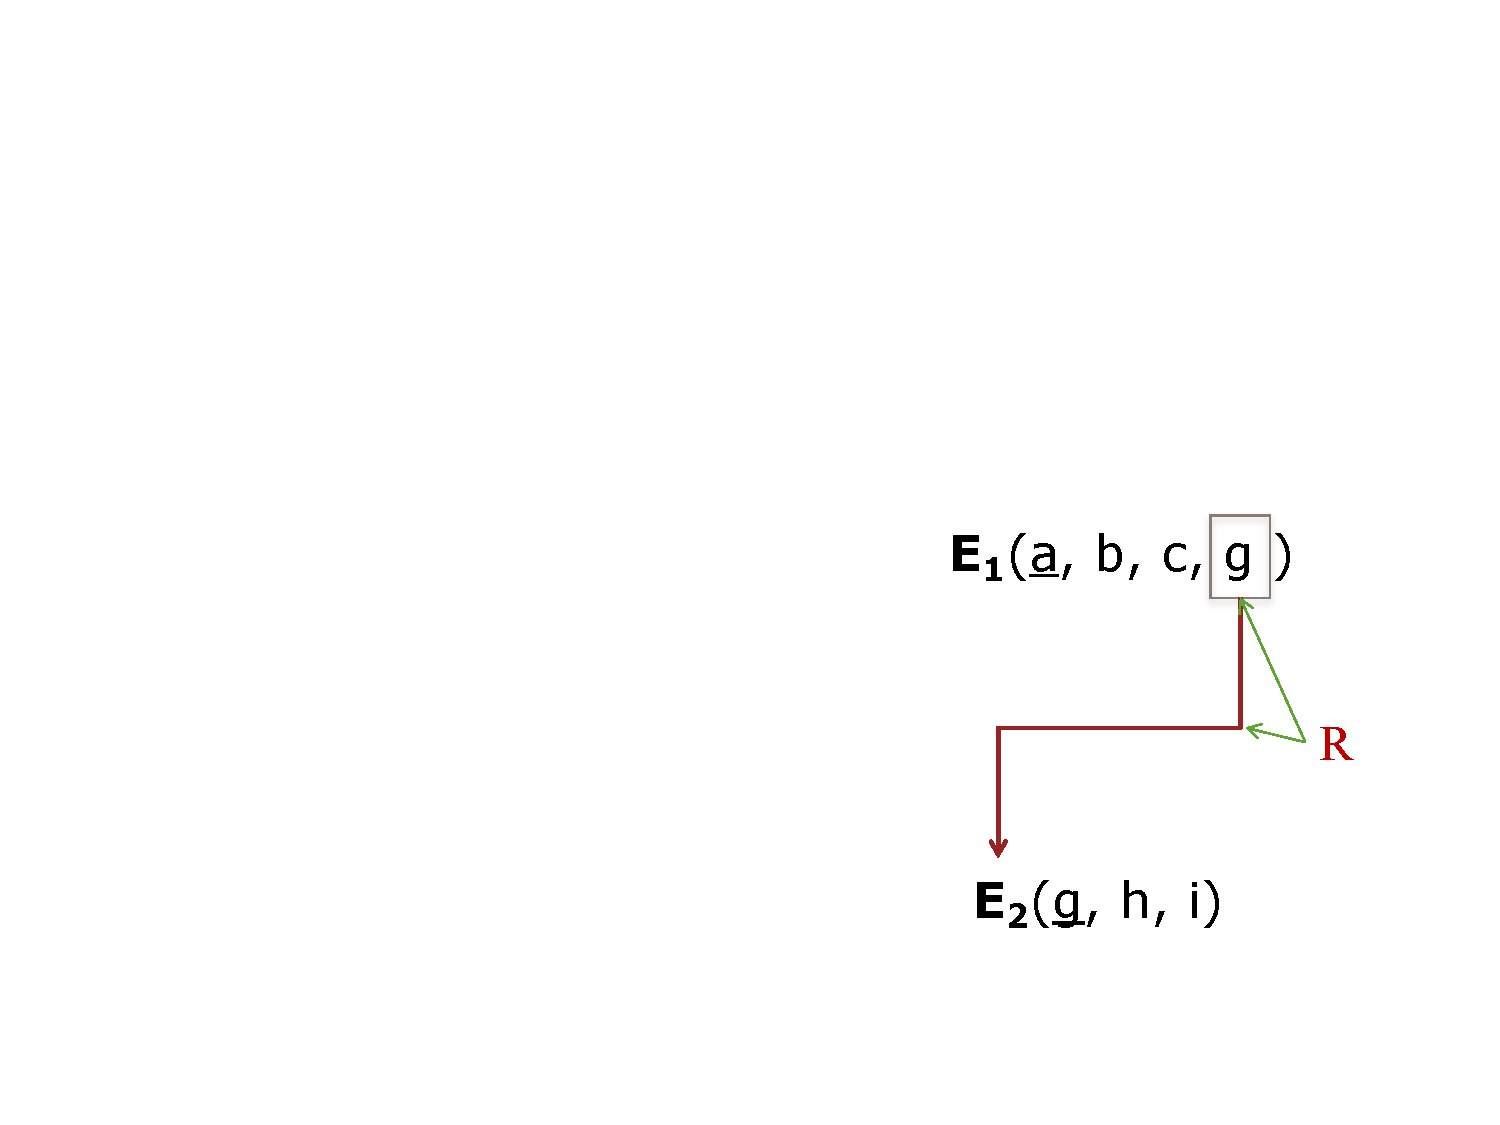
\includegraphics[width=0.3\textwidth]{img/relazionale_uno_a_molti2.pdf}
	\end{figure}

	\newpage
	
	\subsubsection{Relazione uno a uno}
	
	La \textcolor{Red3}{\textbf{\underline{relazione uno a uno}}} è caratterizzata dal fatto che entrambe le entità hanno cardinalità $\left(1,1\right)$.
	
	\begin{figure}[!htp]
		\centering
		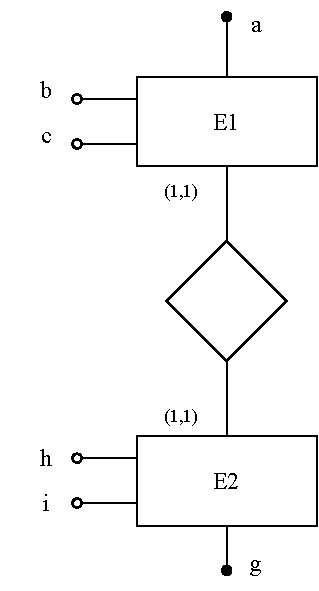
\includegraphics[width=0.5\textwidth]{img/relazionale_uno_a_uno.pdf}
		\caption{Modello E-R di una relazione uno a uno.}
	\end{figure}
	
	\noindent
	Relativo modello relazionale:
	
	\begin{figure}[!htp]
		\centering
		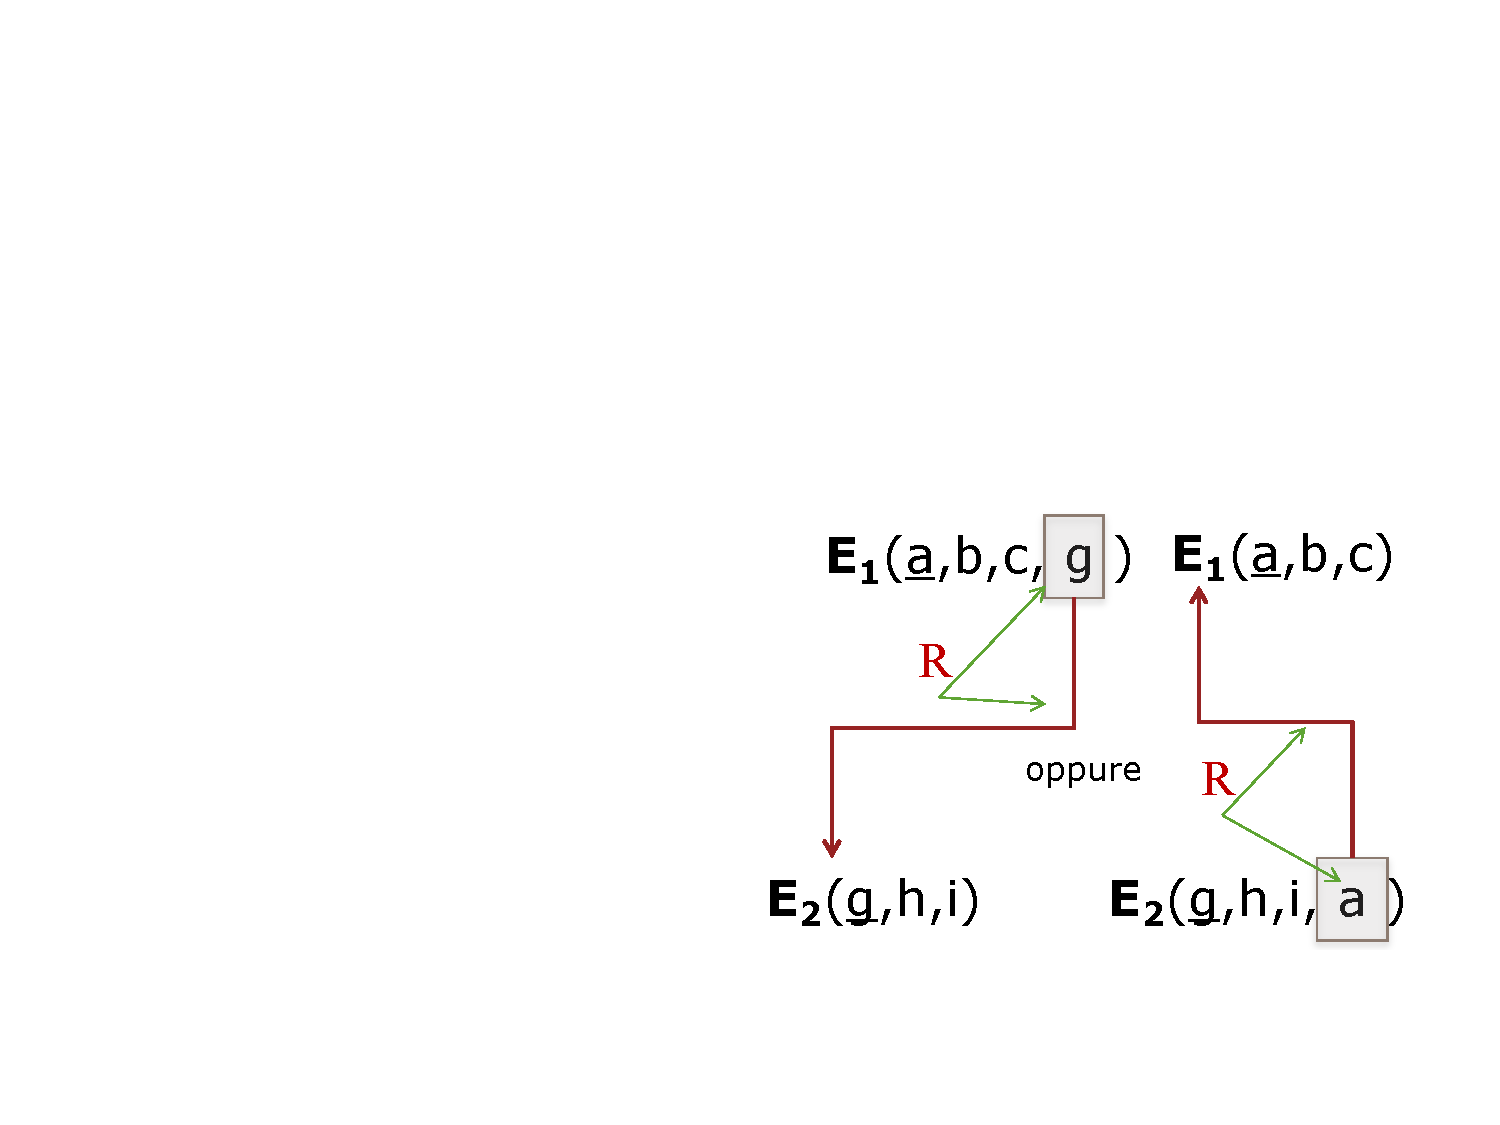
\includegraphics[width=0.4\textwidth]{img/relazionale_uno_a_uno2.pdf}
	\end{figure}

	\newpage
	
	\subsubsection{Relazione molti a molti}
	
	La \textcolor{Red3}{\textbf{\underline{relazione molti a molti}}} è caratterizzata dal fatto che entrambe le entità hanno cardinalità $\left(x,N\right)$ ($x$ può essere qualsiasi valore minimo).
	
	\begin{figure}[!htp]
		\centering
		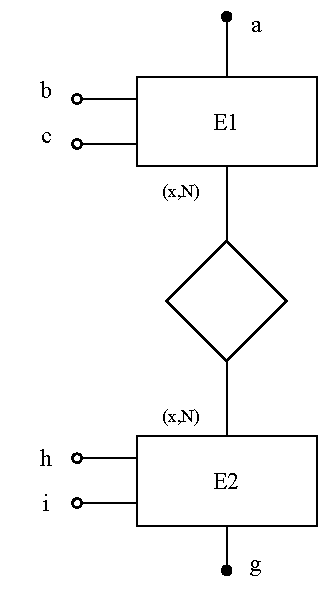
\includegraphics[width=0.5\textwidth]{img/relazionale_molti_a_molti.pdf}
		\caption{Modello E-R di una relazione molti a molti.}
	\end{figure}
	
	\noindent
	Relativo modello relazionale:
	
	\begin{figure}[!htp]
		\centering
		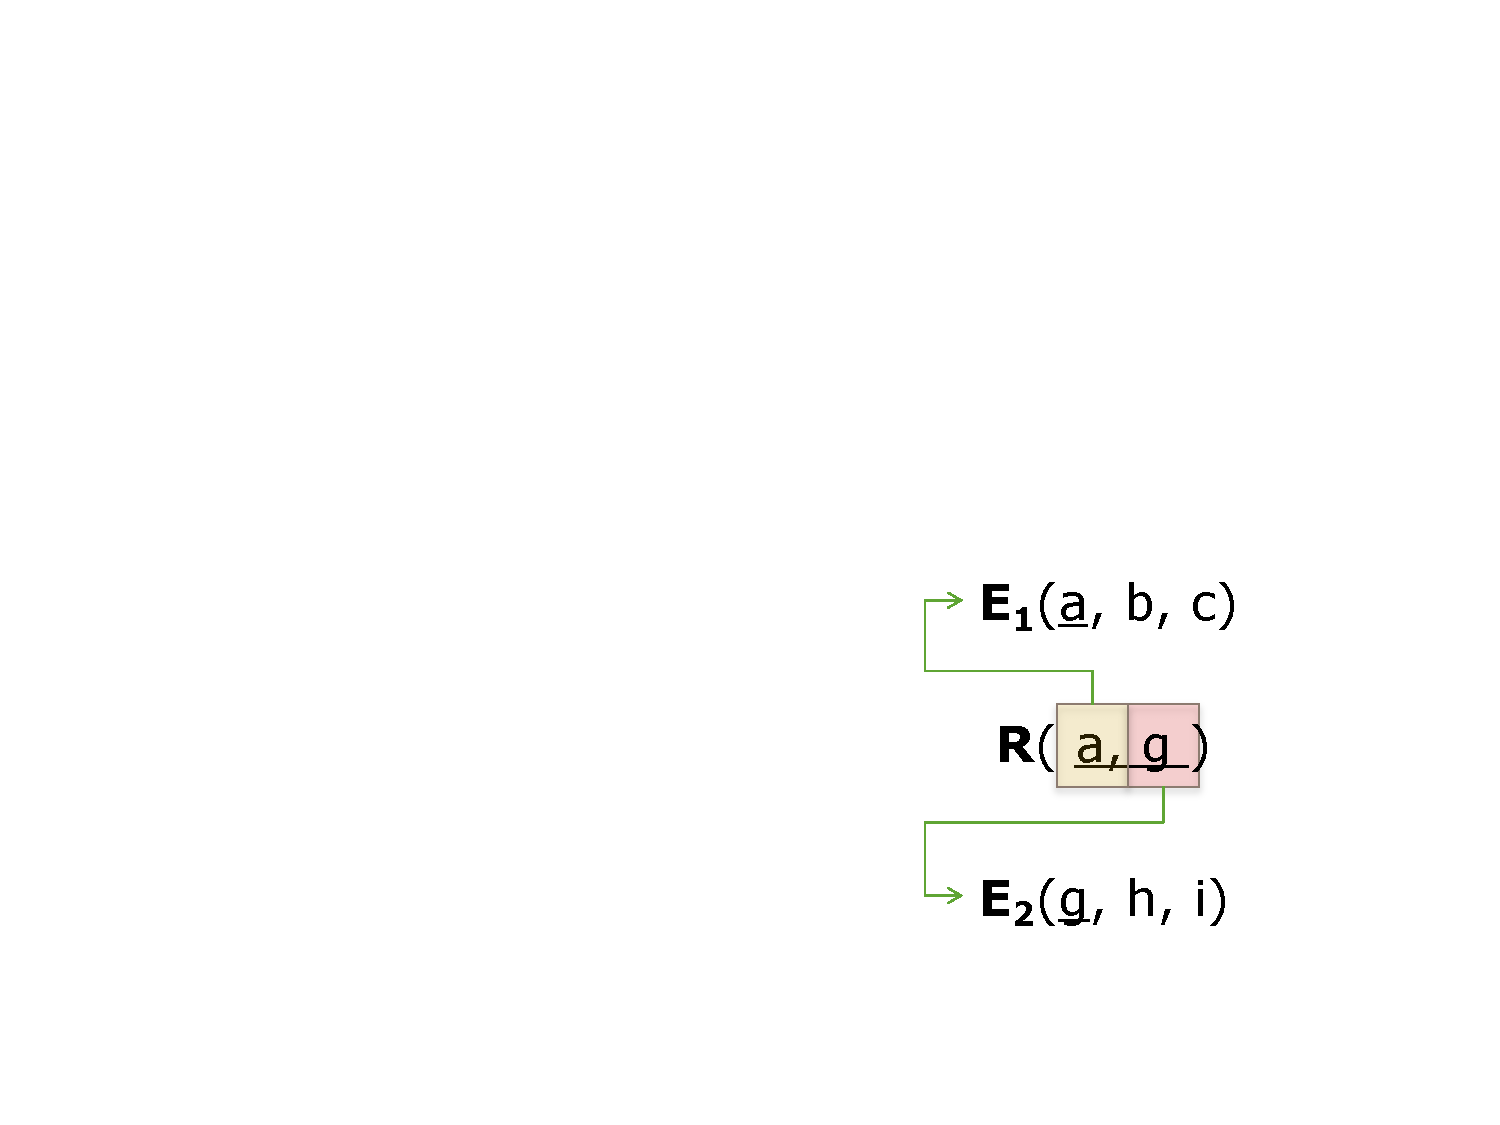
\includegraphics[width=0.2\textwidth]{img/relazionale_molti_a_molti2.pdf}
	\end{figure}

	\newpage
	
	\subsubsection{Relazione uno a molti (identificatore esterno)}
	
	La \textcolor{Red3}{\textbf{\underline{relazione uno a molti con identificatore esterno}}} è caratterizzata dal fatto che un'entità ha cardinalità $\left(1,1\right)$ e l'altra entità ha $\left(x,N\right)$ ($x$ può essere qualsiasi valore minimo).
	
	\begin{figure}[!htp]
		\centering
		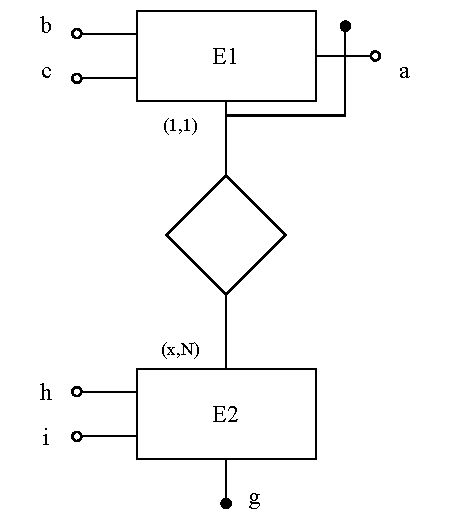
\includegraphics[width=0.5\textwidth]{img/relazionale_uno_a_molti_id_esterno.pdf}
		\caption{Modello E-R di una relazione molti a molti.}
	\end{figure}
	
	\noindent
	Relativo modello relazionale:
	
	\begin{figure}[!htp]
		\centering
		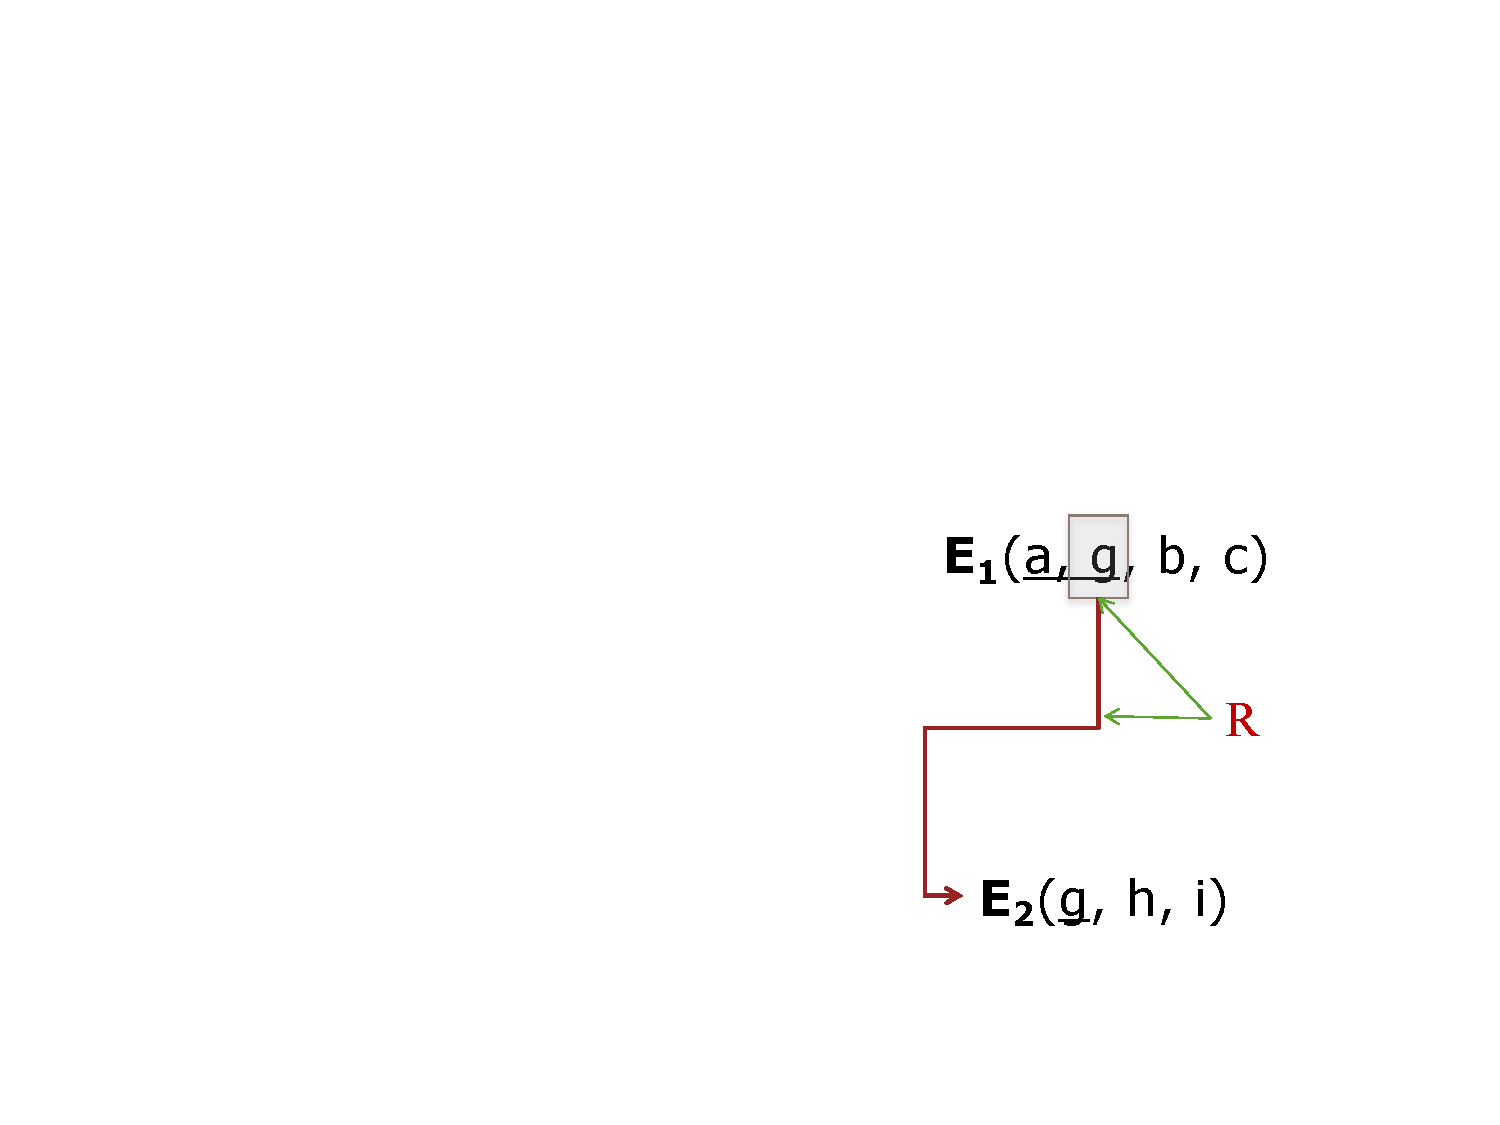
\includegraphics[width=0.2\textwidth]{img/relazionale_uno_a_molti_id_esterno2.pdf}
	\end{figure}

	\newpage
	
	\subsubsection{Relazione uno a molti (attributo sulla relazione)}
	
	La \textcolor{Red3}{\textbf{\underline{relazione uno a molti con un attributo sulla relazione}}} è caratterizzata dal fatto che un'entità ha cardinalità $\left(1,1\right)$, l'altra entità ha $\left(x,N\right)$ ($x$ può essere qualsiasi valore minimo) e un attributo è presente nella relazione.
	
	\begin{figure}[!htp]
		\centering
		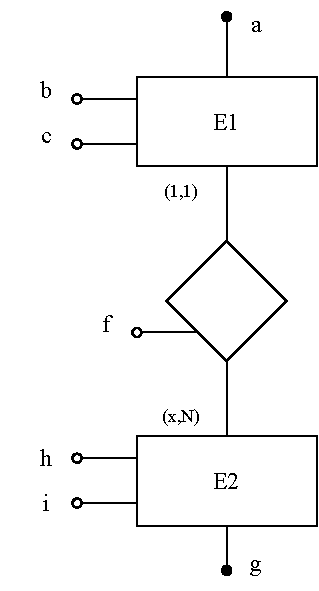
\includegraphics[width=0.4\textwidth]{img/relazionale_uno_a_molti_att_relazione.pdf}
		\caption{Modello E-R di una relazione uno a molti con un attributo sulla relazione esterno.}
	\end{figure}
	
	\noindent
	Relativo modello relazionale:
	
	\begin{figure}[!htp]
		\centering
		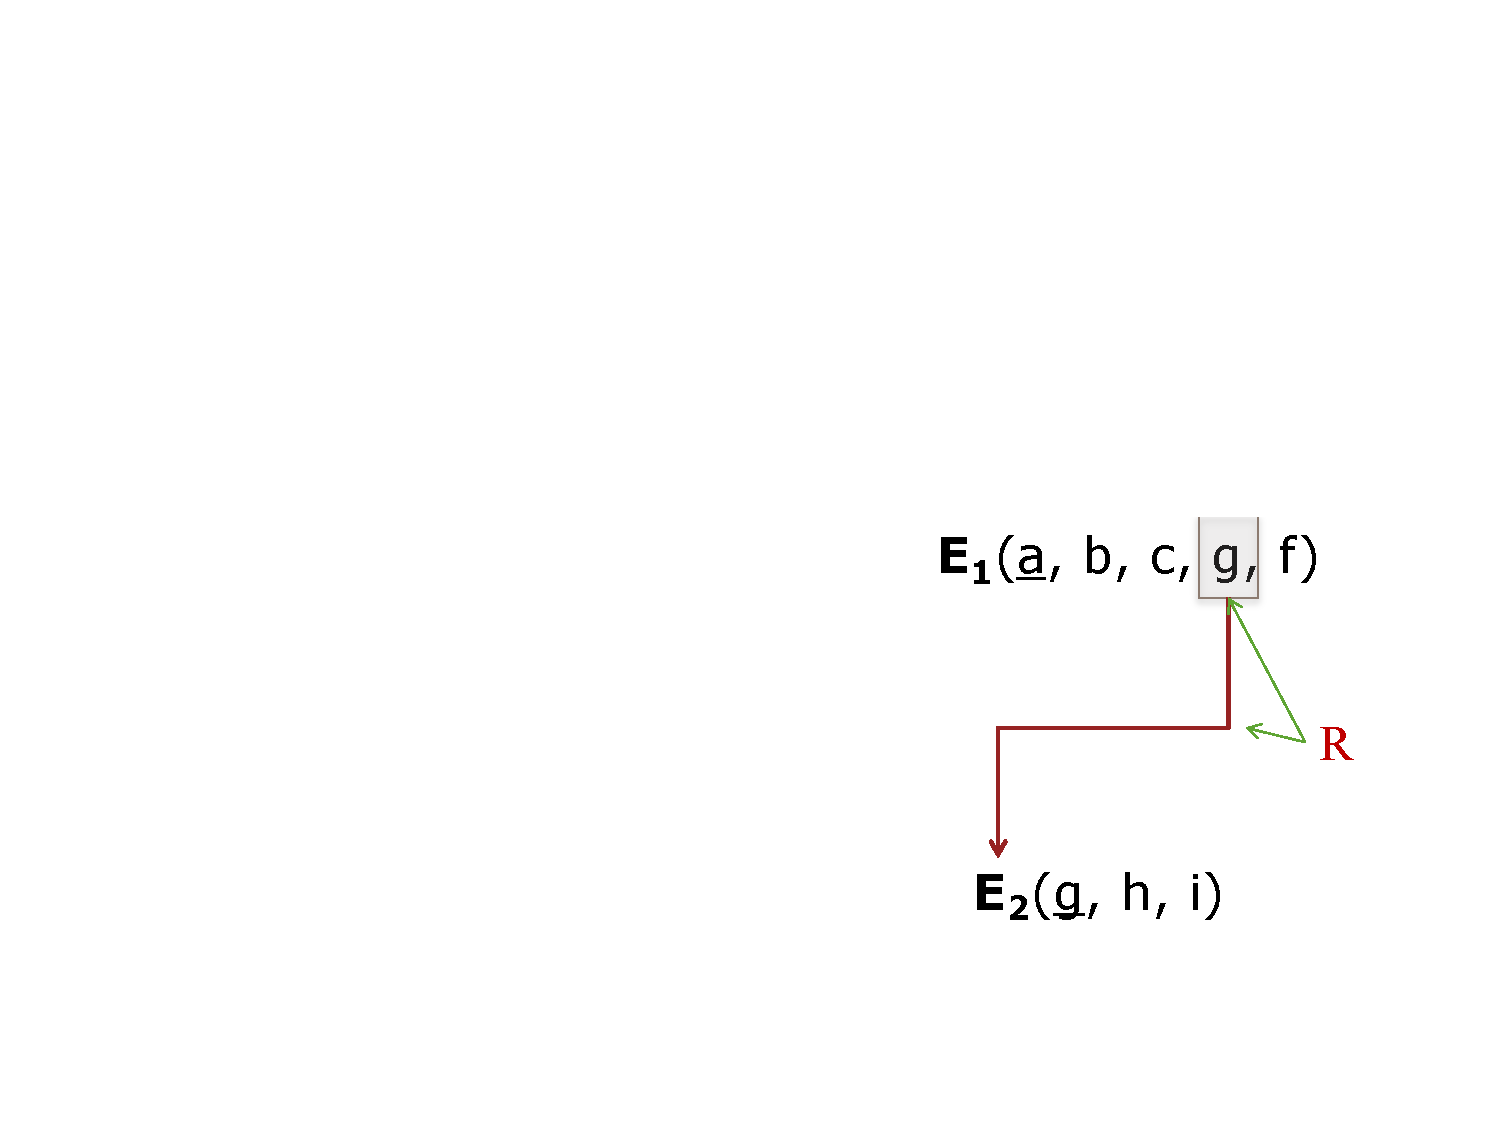
\includegraphics[width=0.2\textwidth]{img/relazionale_uno_a_molti_att_relazione2.pdf}
	\end{figure}

	\newpage
	
	\subsubsection{Relazione uno a uno (una cardinalità minima a zero)}
	
	La \textcolor{Red3}{\textbf{\underline{relazione uno a uno con una cardinalità minima uguale a zero}}} è caratterizzata dal fatto che un'entità ha cardinalità $\left(0,1\right)$, l'altra entità ha $\left(1,1\right)$.
	
	\begin{figure}[!htp]
		\centering
		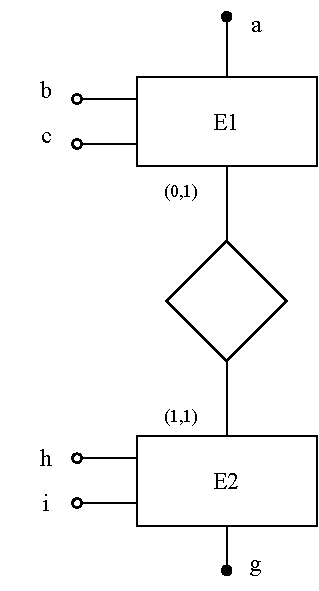
\includegraphics[width=0.4\textwidth]{img/relazionale_uno_a_uno_card_minima_0.pdf}
		\caption{Modello E-R di una relazione uno a uno con una cardinalità minima uguale a zero.}
	\end{figure}
	
	\noindent
	Relativo modello relazionale:
	
	\begin{figure}[!htp]
		\centering
		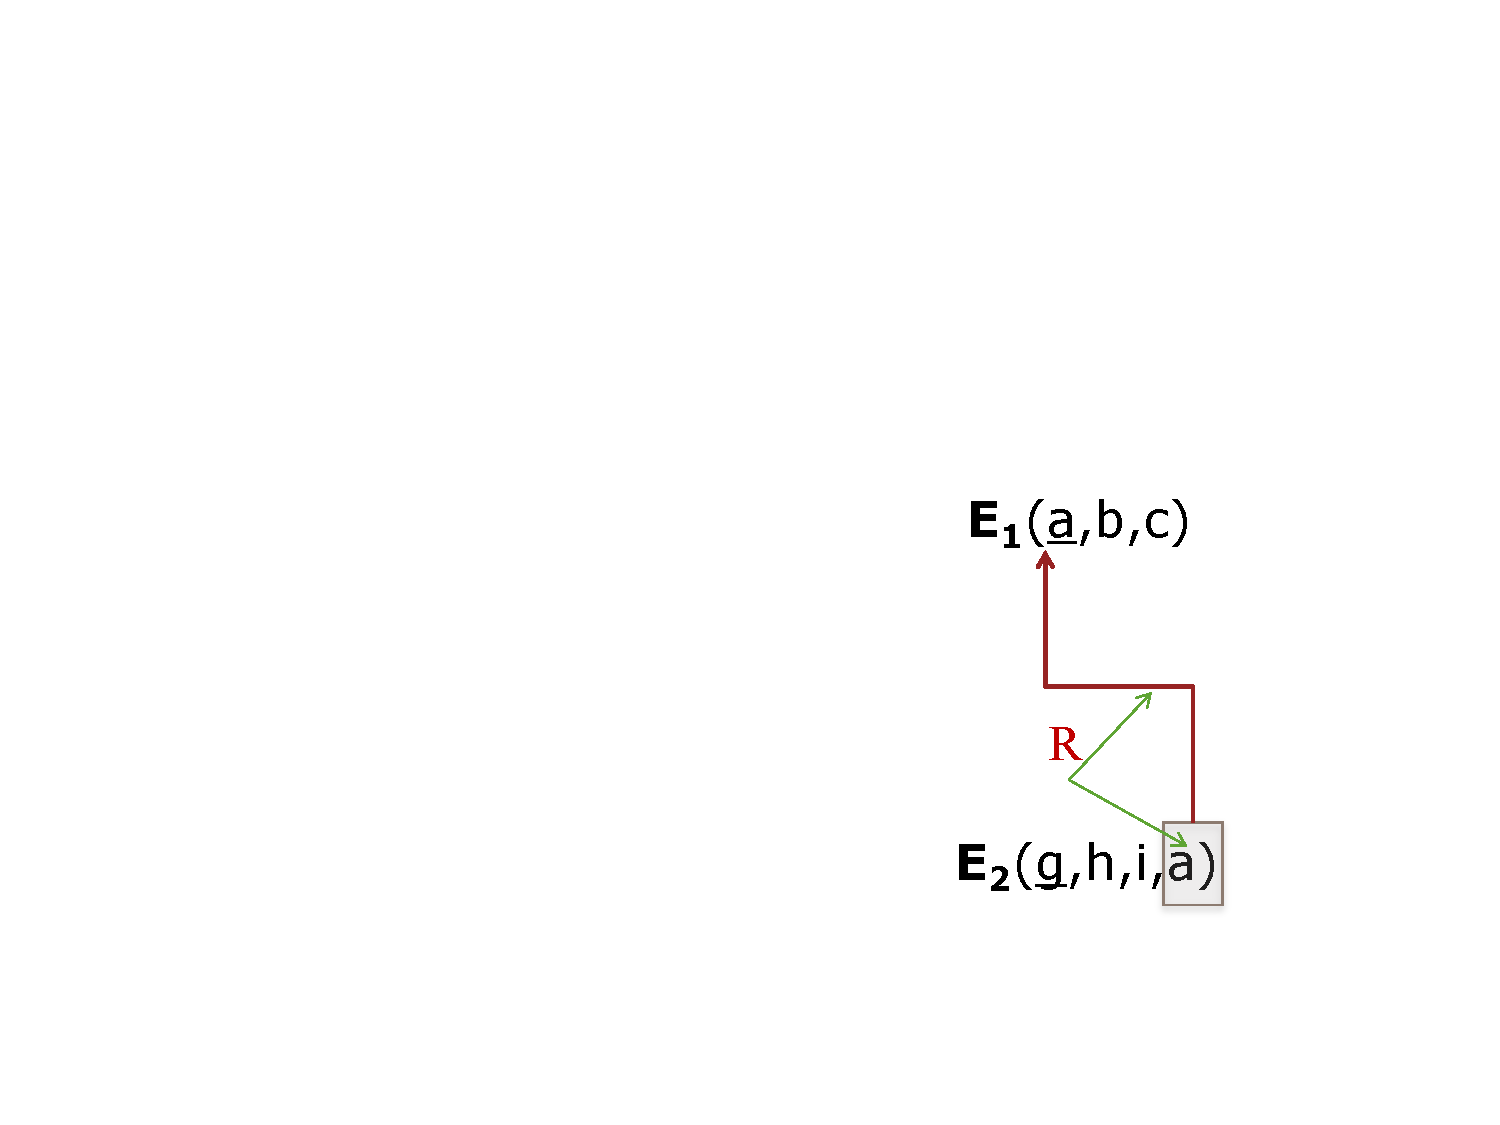
\includegraphics[width=0.2\textwidth]{img/relazionale_uno_a_uno_card_minima_02.pdf}
	\end{figure}

	\newpage
	
	\subsubsection{Relazione uno a uno (entrambe cardinalità minima a zero)}
	
	La \textcolor{Red3}{\textbf{\underline{relazione uno a uno con entrambe le cardinalità minima uguale a zero}}} è caratterizzata dal fatto che un'entità ha cardinalità $\left(0,1\right)$, l'altra entità ha $\left(0,1\right)$.
	
	\begin{figure}[!htp]
		\centering
		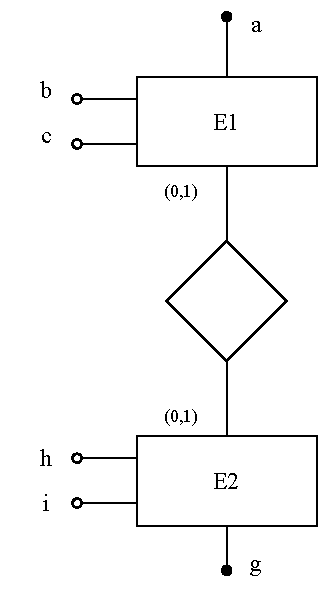
\includegraphics[width=0.4\textwidth]{img/relazionale_uno_a_uno_card_minime_0.pdf}
		\caption{Modello E-R di una relazione uno a uno con entrambe le cardinalità minima uguale a zero.}
	\end{figure}
	
	\noindent
	Relativo modello relazionale:
	
	\begin{figure}[!htp]
		\centering
		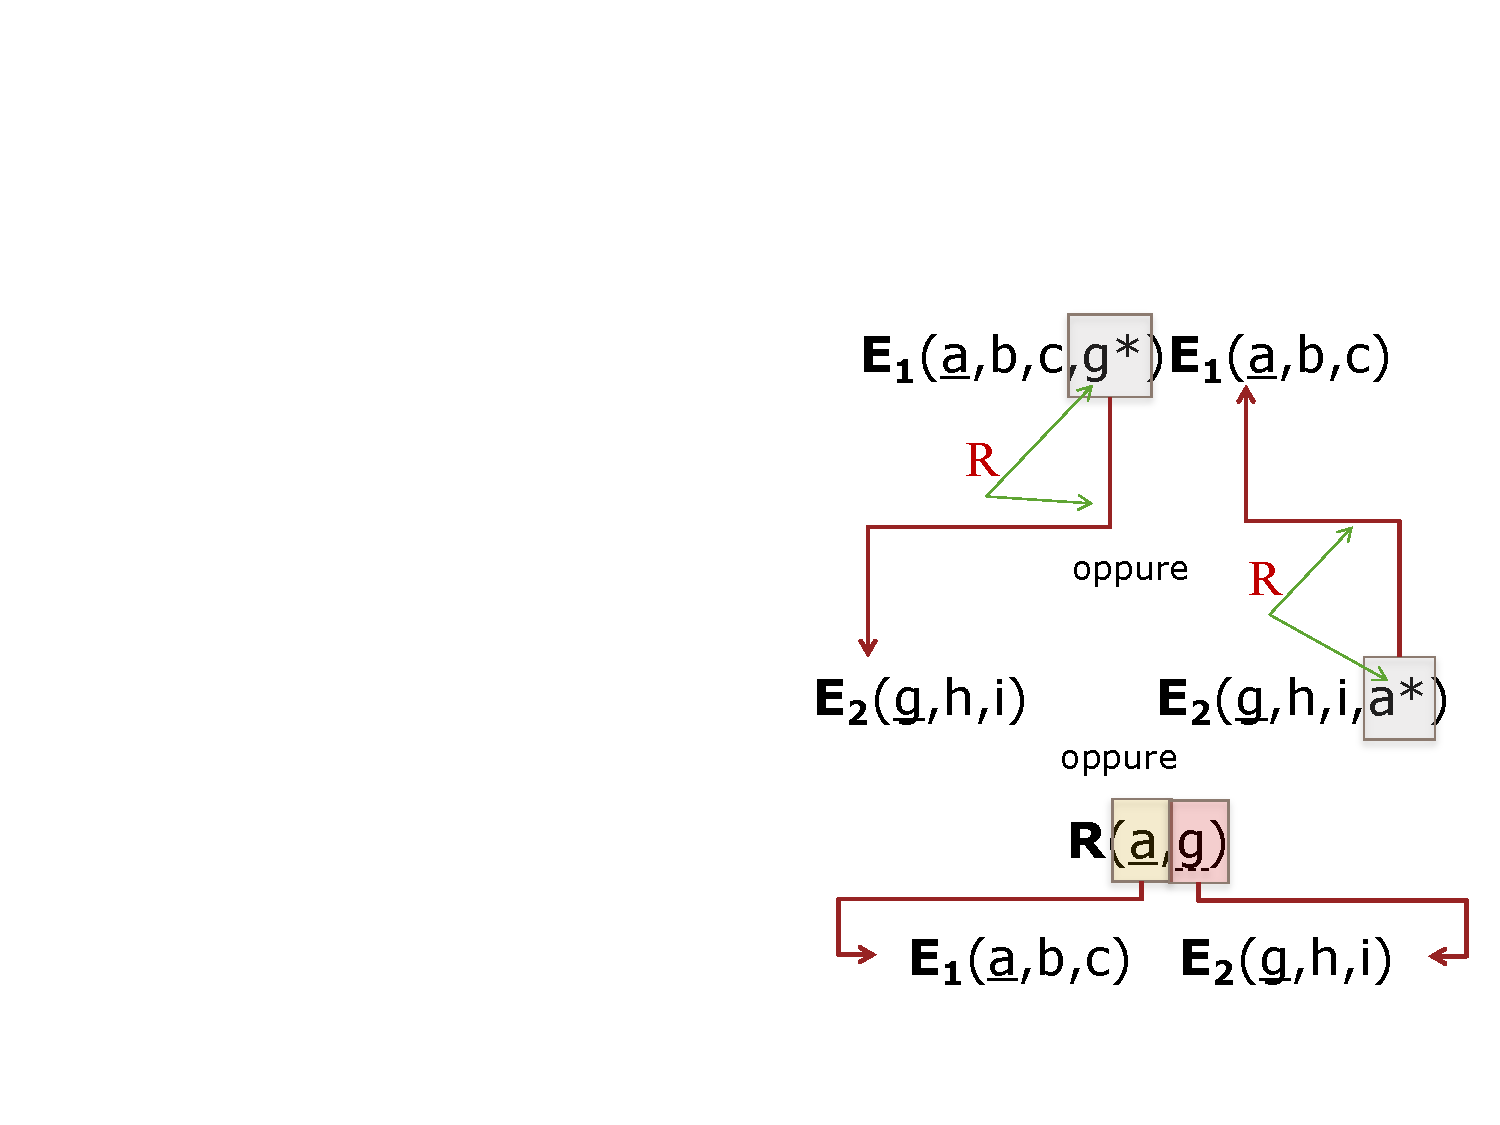
\includegraphics[width=0.4\textwidth]{img/relazionale_uno_a_uno_card_minime_02.pdf}
	\end{figure}

	\newpage
	
	\subsubsection{Relazione molti a molti (attributo sulla relazione)}
	
	La \textcolor{Red3}{\textbf{\underline{relazione molti a molti con un attributo sulla relazione}}} è caratterizzata dal fatto che un'entità ha cardinalità $\left(x,N\right)$, l'altra entità ha $\left(x,N\right)$ ($x$ può essere qualsiasi valore minimo) e un attributo è presente nella relazione.
	
	\begin{figure}[!htp]
		\centering
		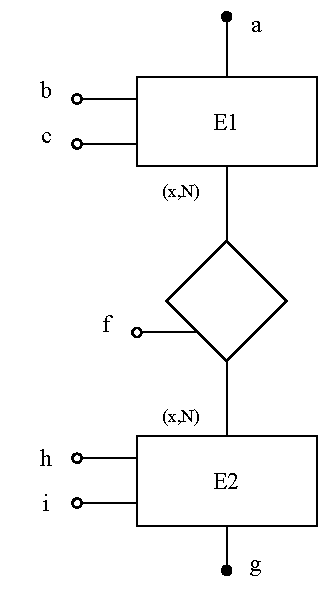
\includegraphics[width=0.4\textwidth]{img/relazionale_molti_a_molti_att_relazione.pdf}
		\caption{Modello E-R di una relazione molti a molti con un attributo sulla relazione esterno.}
	\end{figure}
	
	\noindent
	Relativo modello relazionale:
	
	\begin{figure}[!htp]
		\centering
		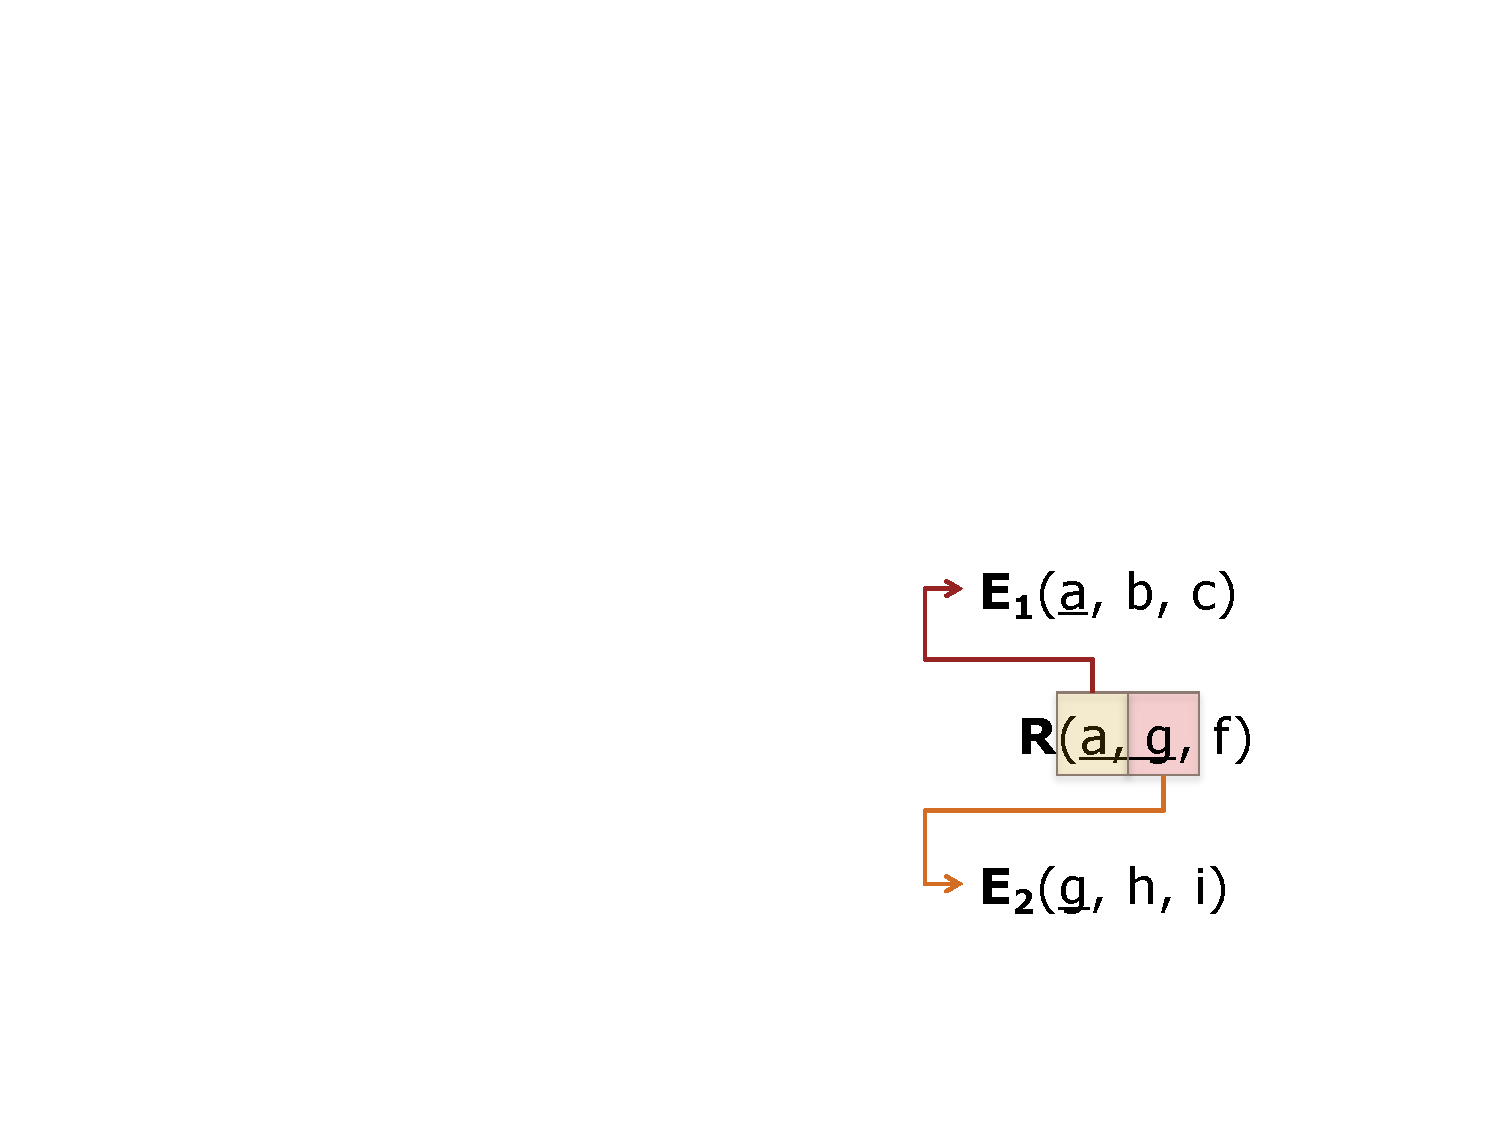
\includegraphics[width=0.25\textwidth]{img/relazionale_molti_a_molti_att_relazione2.pdf}
	\end{figure}

	\newpage
	
	\subsubsection{Relazione molti a molti (identificatori con più attributi)}
	
	La \textcolor{Red3}{\textbf{\underline{relazione molti a molti con identificatori con più attributi}}} è caratterizzata dal fatto che un'entità ha cardinalità $\left(x,N\right)$, l'altra entità ha $\left(x,N\right)$ ($x$ può essere qualsiasi valore minimo) e un attributo è presente nella relazione.
	
	\begin{figure}[!htp]
		\centering
		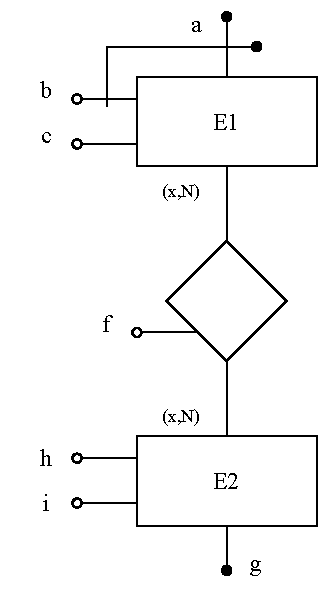
\includegraphics[width=0.4\textwidth]{img/relazionale_molti_a_molti_attributi.pdf}
		\caption{Modello E-R di una relazione molti a molti con identificatori con più attributi.}
	\end{figure}
	
	\noindent
	Relativo modello relazionale:
	
	\begin{figure}[!htp]
		\centering
		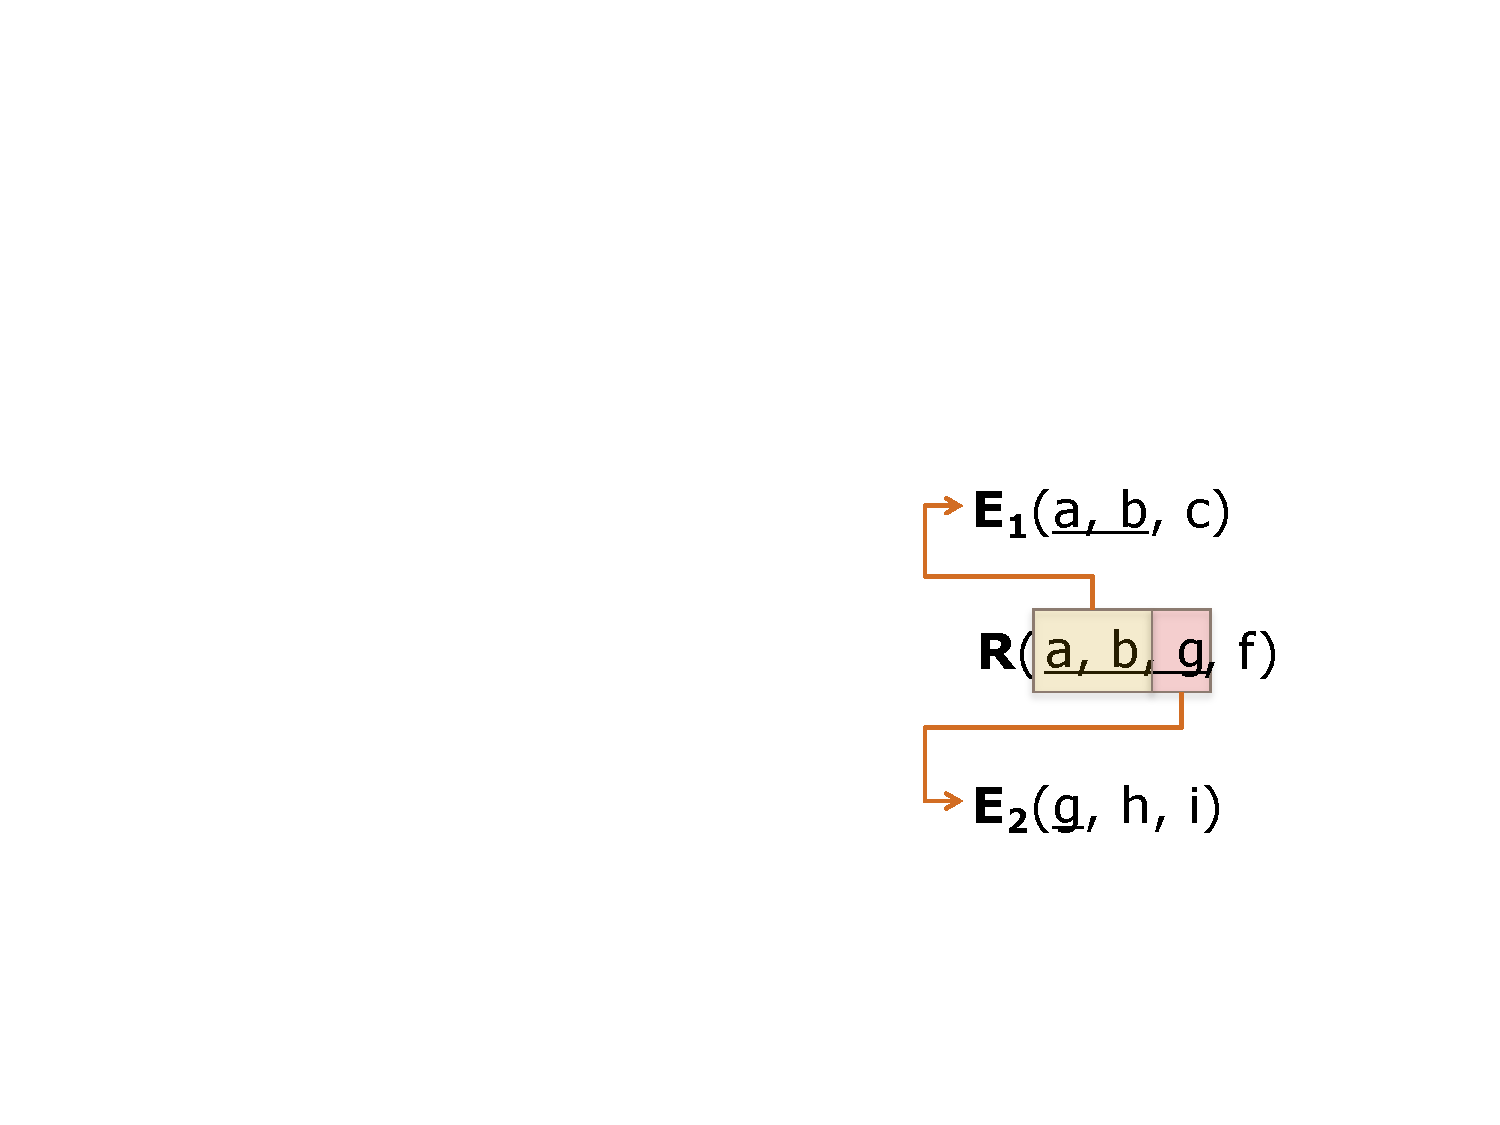
\includegraphics[width=0.25\textwidth]{img/relazionale_molti_a_molti_attributi2.pdf}
	\end{figure}

	\newpage
	
	\subsubsection{Relazione molti a molti (relazione ternaria)}
	
	La \textcolor{Red3}{\textbf{\underline{relazione molti a molti con relazione ternaria}}} è caratterizzata dal fatto che un'entità ha cardinalità $\left(x,N\right)$, l'altra entità ha $\left(x,N\right)$, l'altra entità ancora ha cardinalità $\left(x,N\right)$ ($x$ può essere qualsiasi valore minimo) e un attributo è presente nella relazione.
	
	\begin{figure}[!htp]
		\centering
		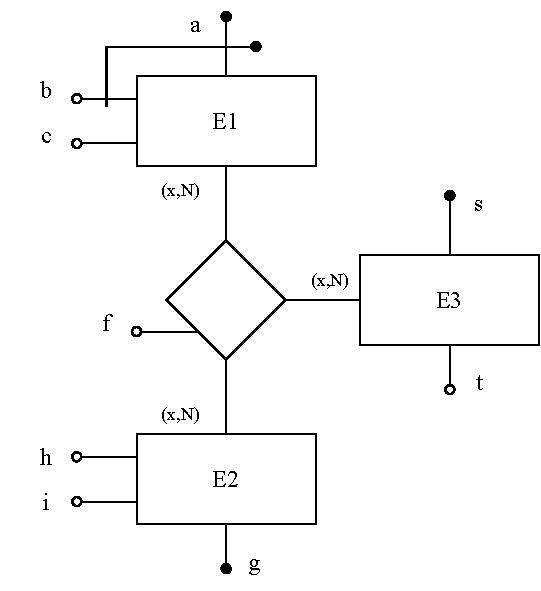
\includegraphics[width=0.6\textwidth]{img/relazionale_molti_a_molti_rel_ternaria.pdf}
		\caption{Modello E-R di una relazione molti a molti con relazione ternaria.}
	\end{figure}
	
	\noindent
	Relativo modello relazionale:
	
	\begin{figure}[!htp]
		\centering
		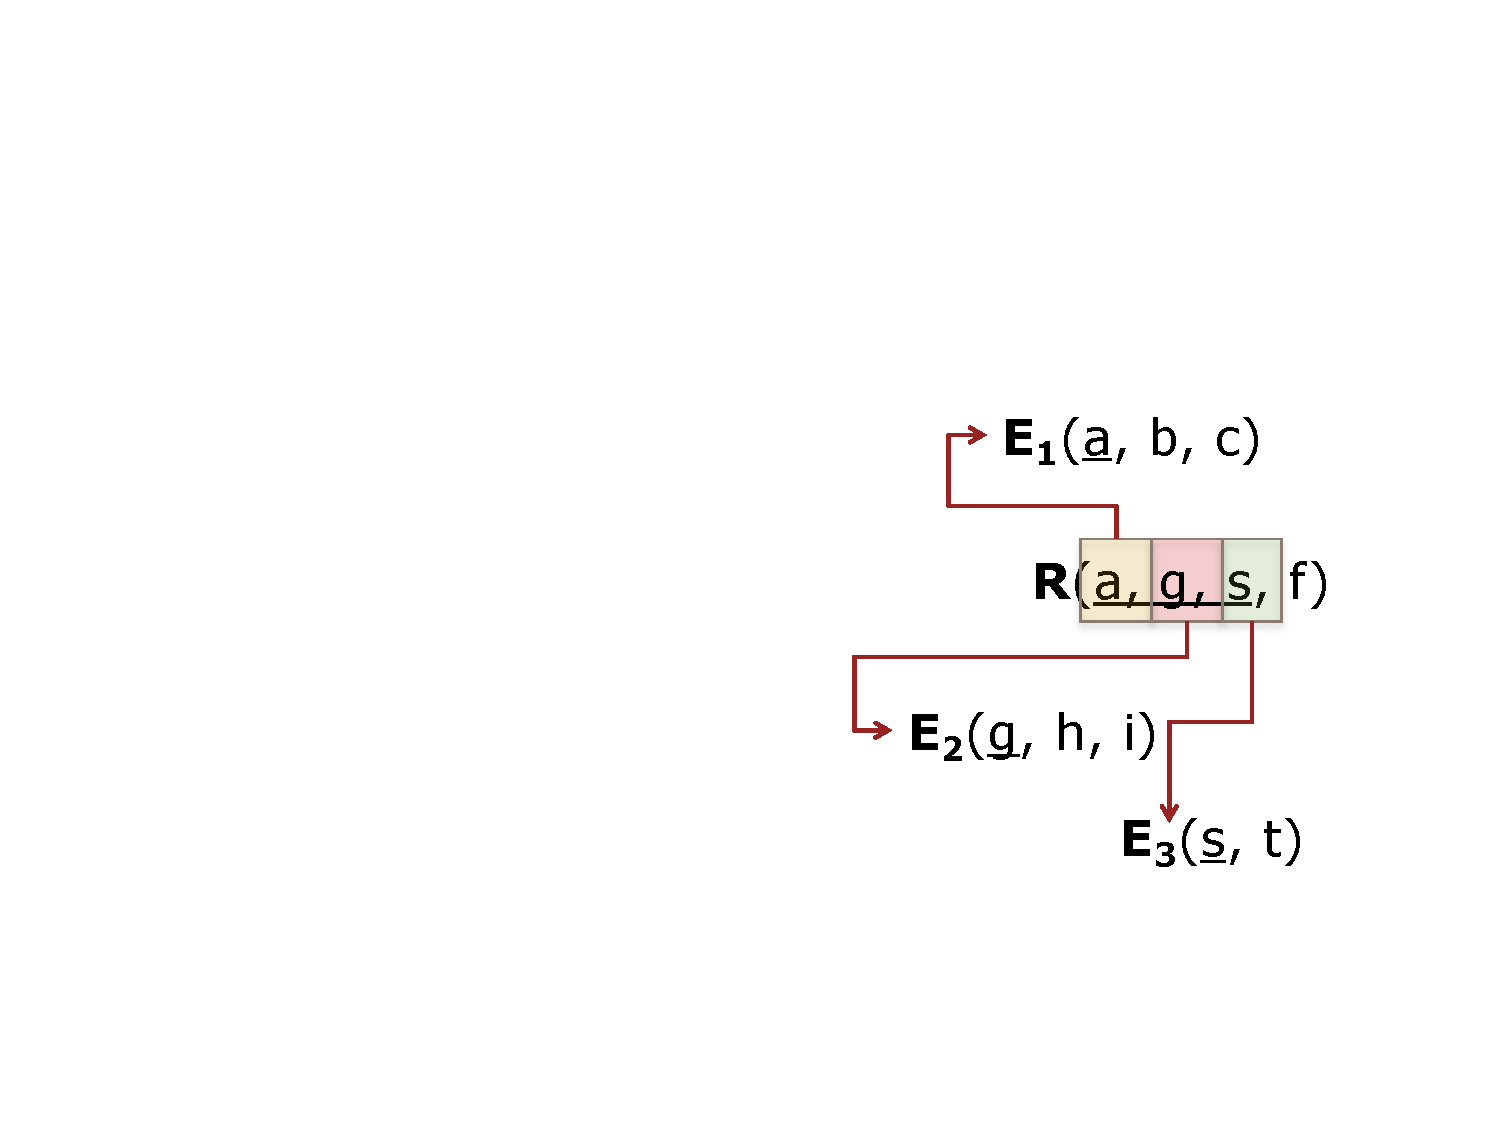
\includegraphics[width=0.32\textwidth]{img/relazionale_molti_a_molti_rel_ternaria2.pdf}
	\end{figure}

	\newpage
	
	\subsubsection{Relazione molti a molti (relazione ternaria e cardinalità uno a uno)}
	
	La \textcolor{Red3}{\textbf{\underline{relazione molti a molti con relazione ternaria e cardinalità uno a uno}}} è caratterizzata dal fatto che un'entità ha cardinalità $\left(1,N\right)$, l'altra entità ha $\left(x,N\right)$, l'altra entità ancora ha cardinalità $\left(x,N\right)$ ($x$ può essere qualsiasi valore minimo) e un attributo è presente nella relazione.
	
	\begin{figure}[!htp]
		\centering
		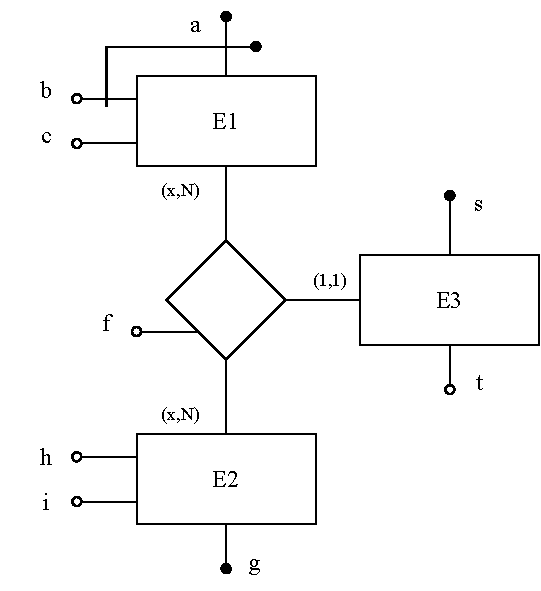
\includegraphics[width=0.6\textwidth]{img/relazionale_molti_a_molti_rel_ternaria_card.pdf}
		\caption{Modello E-R di una relazione molti a molti con relazione ternaria.}
	\end{figure}
	
	\noindent
	Relativo modello relazionale:
	
	\begin{figure}[!htp]
		\centering
		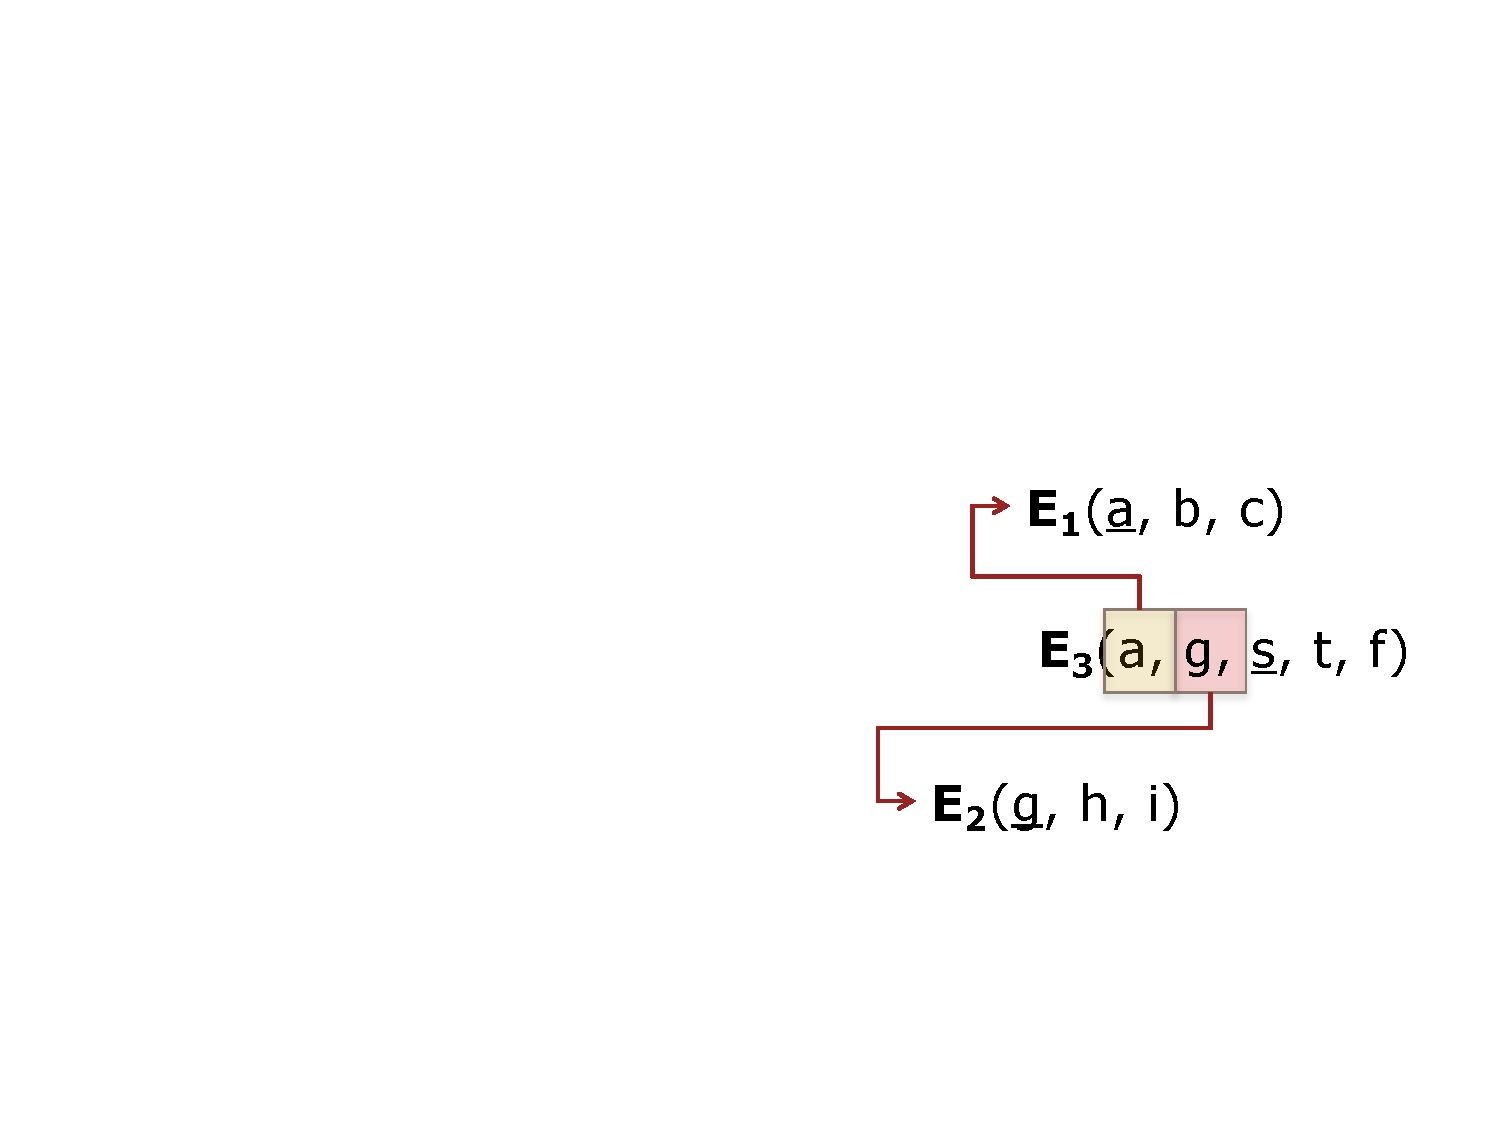
\includegraphics[width=0.4\textwidth]{img/relazionale_molti_a_molti_rel_ternaria_card2.pdf}
	\end{figure}
	
	\newpage
	
	\section{Algebra relazionale}
	
	L'\textcolor{Red3}{\textbf{\underline{algebra relazionale}}} è un linguaggio procedurale, basato su concetti di tipo algebrico. Esso è costituito da un insieme di operatori, definiti su relazioni e che producono ancora relazioni come risultati. I vari operatori sono:
	
	\begin{itemize}
		\item \textbf{Insiemistici}
		\begin{itemize}
			\item \emph{Unione}
			\item \emph{Intersezione}
			\item \emph{Differenza}
		\end{itemize}
	
		\item \textbf{Specifici}
		\begin{itemize}
			\item \emph{Ridenominazione}
			\item \emph{Selezione}
			\item \emph{Proiezione}
		\end{itemize}
		
		\item \textbf{Più importante} \emph{join}
		\begin{itemize}
			\item \emph{Join naturale}
			\item \emph{Prodotto}
			\item \emph{Cartesiano}
			\item \emph{Semijoin}
			\item \emph{Theta-join}
		\end{itemize}
	\end{itemize}

	\noindent
	In altre parole, l'algebra relazione è un insieme di \textbf{operatori} su \textbf{relazioni}. Dato che le relazioni sono insiemi, ha senso definire su di esse gli operatori insiemistici come l'unione, la differenza e l'intersezione
	
	\newpage
	
	\subsection{Insiemistici}

	\subsubsection{Unione}
	
	L'\textcolor{Red3}{\textbf{\underline{unione}}} di due relazioni $r_{1}$ e $r_{2}$ definite sullo stesso insieme di attributi $X$ è indicata con $r_{1} \cup r_{2}$ ed è una relazione ancora su $X$ contenente le tuple che appartengono a $r_{1}$ oppure a $r_{2}$, oppure a entrambe.\newline
	
	\noindent
	La \textbf{cardinalità}, ovvero il numero di tuple contenute nella relazione del risultato:
	
	\begin{equation*}
		\max\left(|r_{1}|, |r_{2}|\right) \le \left|r_{1} \cup r_{2}\right| \le |r_{1}| + |r_{2}|
	\end{equation*}
	
	\noindent
	\textcolor{Green4}{\textbf{\emph{Esempio}}}
	
	\begin{figure}[!htp]
		\centering
		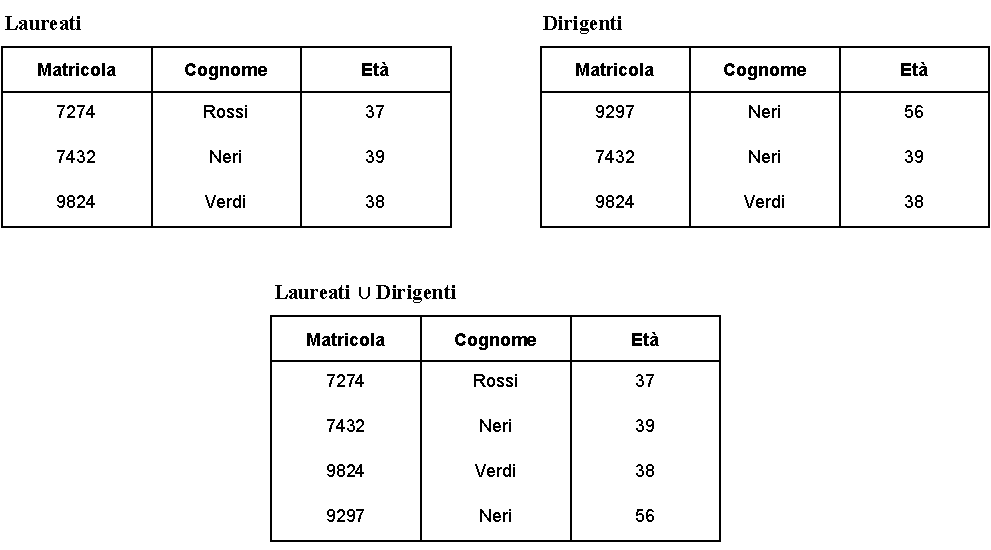
\includegraphics[width=\textwidth]{img/unione.pdf}
	\end{figure}

	\newpage
	
	\subsubsection{Intersezione}
	
	L'\textcolor{Red3}{\textbf{\underline{intersezione}}} di $r_{1}\left(X\right)$ e $r_{2}\left(X\right)$ è indicata con $r_{1} \cap r_{2}$ ed è una relazione su $X$ contenente le tuple che appartengono sia a $r_{1}$ sia a $r_{2}$.\newline
	
	\noindent
	La \textbf{cardinalità}, ovvero il numero di tuple contenute nella relazione del risultato:
	
	\begin{equation*}
		0 \le \left|r_{1} \cap r_{2}\right| \le \min\left(|r_{1}|, |r_{2}|\right)
	\end{equation*}
	
	\noindent
	\textcolor{Green4}{\textbf{\emph{Esempio}}}
	
	\begin{figure}[!htp]
		\centering
		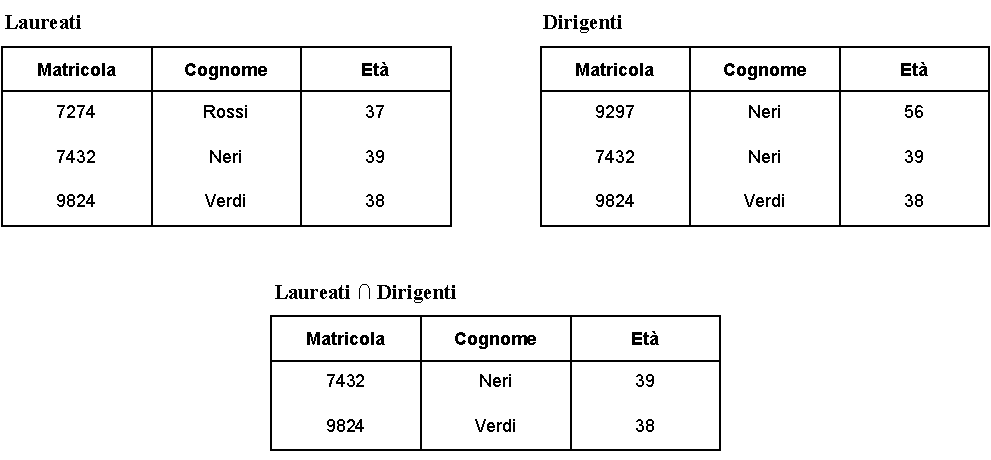
\includegraphics[width=\textwidth]{img/intersezione.pdf}
	\end{figure}

%	\newpage
	
	\subsubsection{Differenza}
	
	La \textcolor{Red3}{\textbf{\underline{differenza}}} di $r_{1}\left(X\right)$ e $r_{2}\left(X\right)$ è indicata con $r_{1} - r_{2}$ ed è una relazione su $X$ contenente le tuple che appartengono a $r_{1}$ e non appartengono a $r_{2}$.\newline
	
	\noindent
	La \textbf{cardinalità}, ovvero il numero di tuple contenute nella relazione del risultato:
	
	\begin{equation*}
		0 \le \left|r_{1} - r_{2}\right| \le |r_{1}|
	\end{equation*}

	\noindent
	\textcolor{Green4}{\textbf{\emph{Esempio}}}
	
	\begin{figure}[!htp]
		\centering
		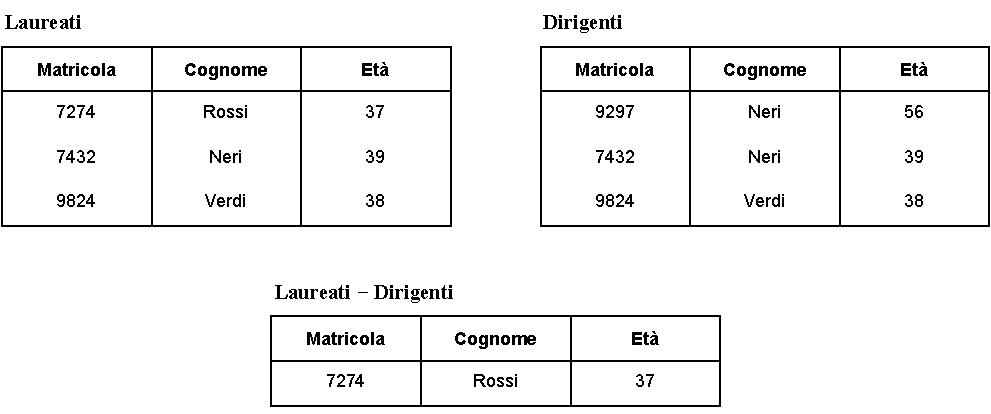
\includegraphics[width=\textwidth]{img/differenza.pdf}
	\end{figure}

	\newpage
	
	\subsection{Specifici}
	
	\subsubsection{Ridenominazione}
	
	L'\textcolor{Red3}{\textbf{\underline{obbiettivo}}} di questo operatore è risolvere le limitazioni degli operatori insiemistici. Infatti, esso \textbf{adegua i nomi degli attributi}, a seconda delle necessità, in particolare alla fine di facilitare le operazioni insiemistiche. Ovviamente, la ridenominazione avviene solamente sugli attributi, il \textbf{contenuto} rimane \textbf{inalterato}.\newline
	
	\noindent
	Il simbolo che lo rappresenta è la lettera greca rho $\rho$. \textbf{Al pedice viene inserita la ridenominazione, a destra il nome dell'attributo da rinominare e a sinistra il nuovo nome dell'attributo}. In generale, sia $r$ una relazione definita sull'insieme di attributi $X$ e sia $Y$ un (altro) insieme di attributi con la stessa cardinalità. Inoltre, siano $A_{1} A_{2} ... A_{k}$ e $B_{1} B_{2} ... B_{k}$ rispettivamente un ordinamento per gli attributi in $X$ e un ordinamento per quelli in $Y$. Allora la ridenominazione:
	
	\begin{equation*}
		\rho_{B_{1}B_{2} ... B_{k} \leftarrow A_{1}A_{2} ... A_{k}} \left(r\right)
	\end{equation*}

	\noindent
	Contiene una tupla $t'$ per ciascuna tupla $t$ in $r$, definita come segue: $t'$ è una tupla su $Y$ e $t\left[B_{i}\right] = t\left[A_{i}\right]$, per $i = 1, ..., k$.\newline
	
	\noindent
	La definizione conferma che ciò che cambia sono i nomi degli attributi, mentre i valori rimangono inalterati e vengono associati ai nuovi attributi.\newline
	
	\noindent
	\textcolor{Green4}{\textbf{\emph{Esempio}}}
	
	\begin{figure}[!htp]
		\centering
		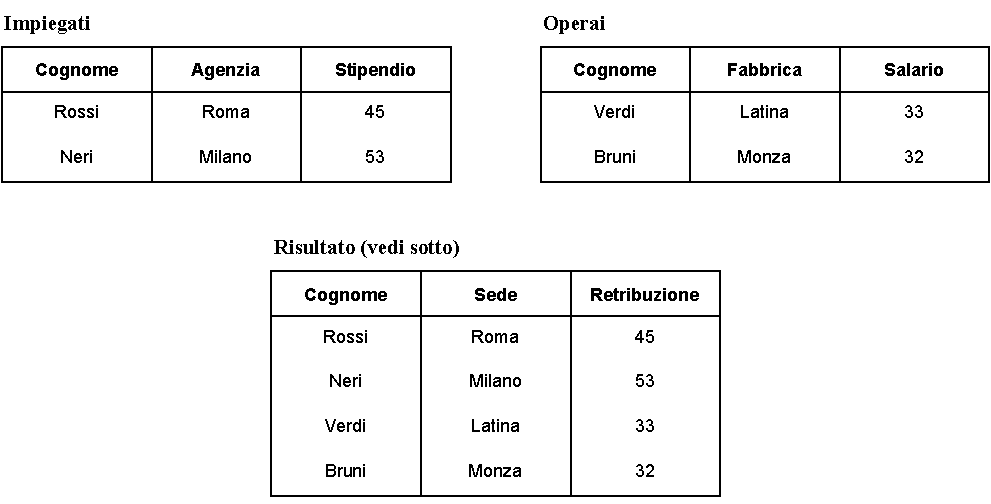
\includegraphics[width=\textwidth]{img/ridenominazione.pdf}
	\end{figure}

	\noindent
	Il risultato è ottenuto con la seguente operazione:
	
	\begin{equation*}
		\rho_{\text{ Sede, Retribuzione } \leftarrow \text{ Agenzia, Stipendio}} \left(\text{Impiegati}\right) \cup \rho_{\text{ Sede, Retribuzione } \leftarrow \text{ Fabbrica, Salario}}\left(\text{Operai}\right)
	\end{equation*}

	\newpage
	
	\subsubsection{Selezione}
	
	La selezione produce una porzione dell'operando. Più precisamente, la \textcolor{Red3}{\textbf{\underline{selezione}}} produce un sottoinsieme delle tuple su tutti gli attributi. Il \textbf{risultato contiene le tuple dell'operando che soddisfano la condizione di selezione}. Quest'ultima viene indicata nel pedice della notazione della selezione, ovvero sigma $\sigma$. Inoltre, le condizioni possono prevedere confronti fra attributi e confronti fra attributi e costanti, e possono essere complesse, ottenute combinando condizioni semplici con i connettivi logici $\lor$ (or), $\land$ (and) e $\lnot$ (not).\newline
	
	\noindent
	In generale, data una relazione $r\left(X\right)$, una \emph{forma proposizionale} $F$ su $X$ è una formula ottenuta combinando, con i connettivi $\land, \lor, \lnot$, condizioni atomiche del tipo $A\theta B$ o $A\theta c$, dove:
	
	\begin{itemize}
		\item $\theta$ è un \textbf{operatore di confronto}, il quale può essere:
		\begin{itemize}
			\item $=$
			\item $\ne$
			\item $>$
			\item $<$
			\item $\ge$
			\item $\le$
		\end{itemize}
	
		\item $A$ e $B$ sono \textbf{attributi} in $X$ sui cui valori il confronto $\theta$ abbia senso;
		
		\item $c$ è una \textbf{costante} \dquotes{compatibile} con il dominio di $A$ (cioè tale che il confronto $\theta$ sia definito).
	\end{itemize}
	
	\noindent
	Data una formula $F$ e una tupla $t$, è definito un valore di verità (cioè \dquotes{vero} o \dquotes{falso}) per $F$ su $t$:
	
	\begin{itemize}
		\item $A \theta B$ è vera su $t$ se $t\left[A\right]$ è in relazione $\theta$ con $t\left[B\right]$, altrimenti è falsa (per esempio, $A = B$ è vera su $t$ se e solo se $t\left[A\right] = t\left[B\right]$);
		
		\item $A \theta c$ è vera su $t$ se $t\left[A\right]$ è in relazione $\theta$ con $c$, altrimenti è falsa;
		
		\item $F_{1} \lor F_{2}, F_{1} \land F_{2}$ e $\lnot F_{1}$ hanno l'usuale significato.
	\end{itemize}

	\noindent
	La \textbf{\underline{definizione}}, in altre parole, è: la \textcolor{Red3}{\textbf{\underline{selezione}}} $\sigma_{F}\left(r\right)$, in cui $r$ è una relazione e $F$ una formula proposizionale, produce una relazione sugli stessi attributi di $r$ che contiene le tuple di $r$ su cui $F$ è vera.
	
	\newpage
	
	\noindent
	\textcolor{Green4}{\textbf{\emph{Esempio 1}}}
	
	\begin{figure}[!htp]
		\centering
		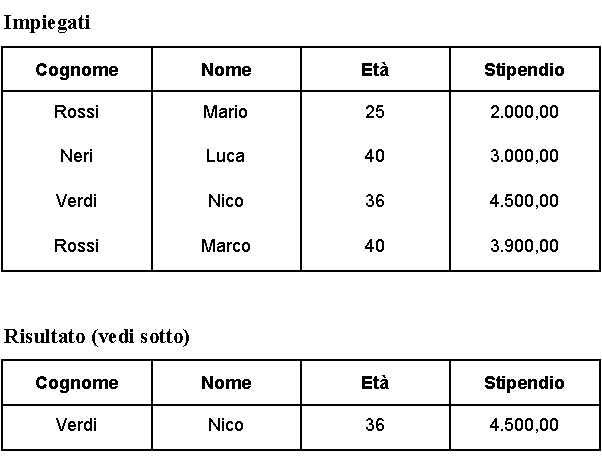
\includegraphics[width=0.8\textwidth]{img/selezione1.pdf}
	\end{figure}

	\noindent
	Il risultato è ottenuto con la seguente operazione:
	
	\begin{equation*}
		\sigma_{\text{Eta } > 30 \land \text{ Stipendio } > 4.000,00}\left(\text{Impiegati}\right)
	\end{equation*}

	\noindent
	\textcolor{Green4}{\textbf{\emph{Esempio 2}}}
	
	\begin{figure}[!htp]
		\centering
		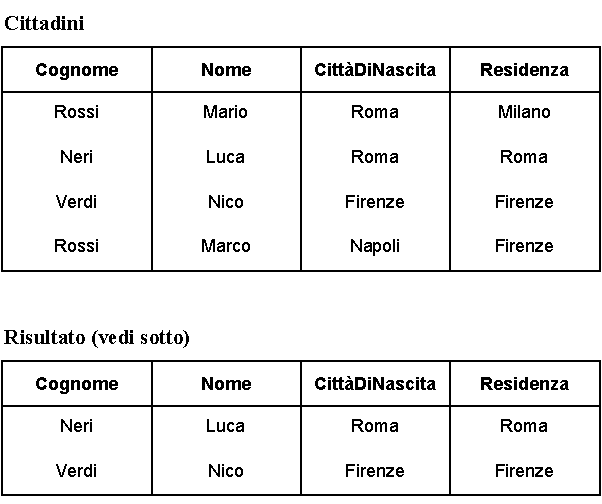
\includegraphics[width=0.8\textwidth]{img/selezione2.pdf}
	\end{figure}

	\noindent
	Il risultato è ottenuto con la seguente operazione:
	
	\begin{equation*}
		\sigma_{\text{CittàDiNascita } = \text{ Residenza}}\left(\text{Cittadini}\right)
	\end{equation*}
	
	\newpage
	
	\subsubsection{Proiezione}
	
	La \textcolor{Red3}{\textbf{\underline{proiezione}}} dà un risultato cui contribuiscono tutte le tuple, ma su un sottoinsieme degli attributi.
	
	Formalmente, dati una relazione $r\left(X\right)$ e un sottoinsieme $Y$ di $X$, la \textbf{proiezione} di $r$ su $Y$ (indicata con $\pi_{Y}\left(r\right)$) è l'insieme di tuple su $Y$ ottenute dalle tuple di $r$ considerando solo i valori su $Y$:
	
	\begin{equation*}
		\pi_{Y}\left(r\right) = \left\{t\left[Y\right] \: | \: t \in r\right\}
	\end{equation*}

	\noindent
	Dagli esempi è chiaro che la proiezione permette di decomporre verticalmente le relazioni.\newline
	
	\noindent
	\textcolor{Green4}{\textbf{\emph{Esempio 1}}}\newline
	
	\noindent
	In questo caso, il risultato della proiezione contiene tante tuple quante l'operando, definite però solo su parte degli attributi.
	
	\begin{figure}[!htp]
		\centering
		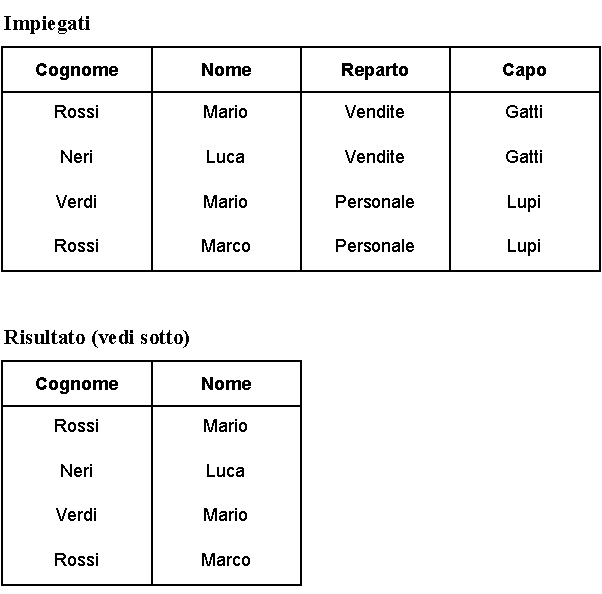
\includegraphics[width=0.9\textwidth]{img/proiezione1.pdf}
	\end{figure}
	
	\noindent
	Il risultato è ottenuto con la seguente operazione:
	
	\begin{equation*}
		\pi_{\text{Cognome, Nome }}\left(\text{Impiegati}\right)
	\end{equation*}

	\newpage
	
	\noindent
	\textcolor{Green4}{\textbf{\emph{Esempio 2}}}\newline
	
	\noindent
	In questo caso, il risultato contiene un numero di tuple inferiore rispetto a quelle dell'operando, perché alcune tuple, avendo uguali valori su tutti gli attributi della proiezione, danno lo stesso contributo alla proiezione stessa. Essendo le relazioni definite come insieme, non possono, per definizione, in esse comparire più tuple uguale fra loro: i contributi \dquotes{collassano} in una sola tupla.
	
	\begin{figure}[!htp]
		\centering
		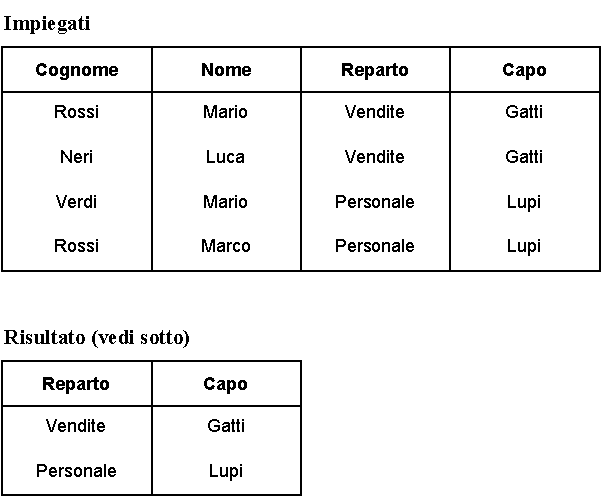
\includegraphics[width=0.9\textwidth]{img/proiezione2.pdf}
	\end{figure}
	
	\noindent
	Il risultato è ottenuto con la seguente operazione:
	
	\begin{equation*}
		\pi_{\text{Reparto, Capo }}\left(\text{Impiegati}\right)
	\end{equation*}
	
	\newpage
	
	\subsection{Join}
	
	L'operatore di \emph{join} consente di correlare dati contenuti in relazioni diverse, confrontando i valori contenuti in esse e utilizzando quindi la caratteristica fondamentale del modello, ovvero quella di essere basta su valori.
	
	Formalmente, due relazione $r_{1}$ e $r_{2}$ di schema $X_{1}$ e $X_{2}$ rispettivamente, gli operatori di \emph{join} generano tuple $t$ nella relazione risultato a partire dalle coppie di tuple $\left(t_{1}, t_{2}\right) \in r_{1} \times r_{2}$ che soddisfano una certa condizione (chiamata \textbf{predicato di join}).
	
	\subsubsection{Join naturale}
	
	Il \textcolor{Red3}{\textbf{\underline{join naturale}}} è un operatore che correla dati in relazioni diverse, sulla base di valori uguali in attributi con lo stesso nome (si veda l'esempio come chiarificatore). Questa operazione viene denotata con il simbolo $\Join$.
	
	Il \textbf{risultato} dell'operatore è una relazione sull'unione degli insiemi di attributi degli operandi e le sue tuple sono ottenute combinando le tuple degli operandi con valori uguali sugli attributi comuni. Nel primo esempio sotto, la prima tupla del \emph{join} deriva dalla combinazione della prima tupla della relazione $r_{1}$ e dalla seconda tupla della relazione $r_{2}$.\newline
	
	\noindent
	Formalmente, il \textbf{join naturale} $r_{1} \Join r_{2}$ di $r_{1}\left(X_{1}\right)$ e $r_{2}\left(X_{2}\right)$ è una relazione definita su $X_{1}X_{2}$ (cioè sull'unione degli insiemi $X_{1}$ e $X_{2}$), come segue:
	
	\begin{equation*}
		r_{1} \Join r_{2} = \left\{t \text{ su } X_{1}X_{2} \:\: | \:\: t\left[X_{1}\right] \in r_{1}, t\left[X_{2}\right] \in r_{2}\right\}
	\end{equation*}

	\noindent
	Si noti che è molto frequente eseguire \emph{join} sulla base di valori della chiave di una delle relazioni coinvolte, esplicitando i riferimenti fra tuple che sono realizzati per mezzo di valori soprattutto valori di chiavi. Osservando l'esempio 2, si vede che ciascuna delle tuple di \textsf{Infrazioni} è stata combinata con una e una sola delle tuple di \textsf{Auto}:
	
	\begin{itemize}
		\item  Una sola perché \textsf{Prov} e \textsf{Numero} formano una chiave di \textsf{Auto};
		\item Almeno una perché è definito il vincolo di integrità referenziale fra \textsf{Prov} e \textsf{Numero} in \textsf{Infrazioni} e (la chiave primaria di) \textsf{Auto}
	\end{itemize}

	\noindent
	Dunque, il \emph{join} ha esattamente tante tuple quante la relazione \textsf{Infrazioni}.
	
	\newpage
	
	\noindent
	\textcolor{Green4}{\textbf{\emph{Esempio 1}}}
	
	\begin{figure}[!htp]
		\centering
		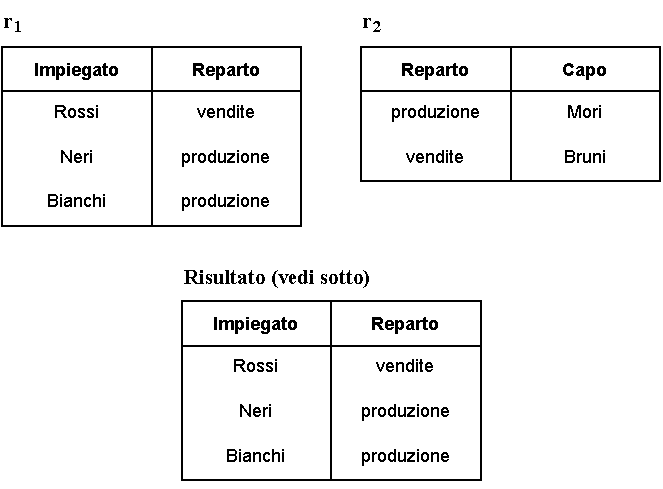
\includegraphics[width=0.65\textwidth]{img/join_naturale1.pdf}
	\end{figure}
	
	\noindent
	Il risultato è ottenuto con la seguente operazione:
	
	\begin{equation*}
		r_{1} \Join r_{2}
	\end{equation*}

	\noindent
	\textcolor{Green4}{\textbf{\emph{Esempio 2}}}
	
	\begin{figure}[!htp]
		\centering
		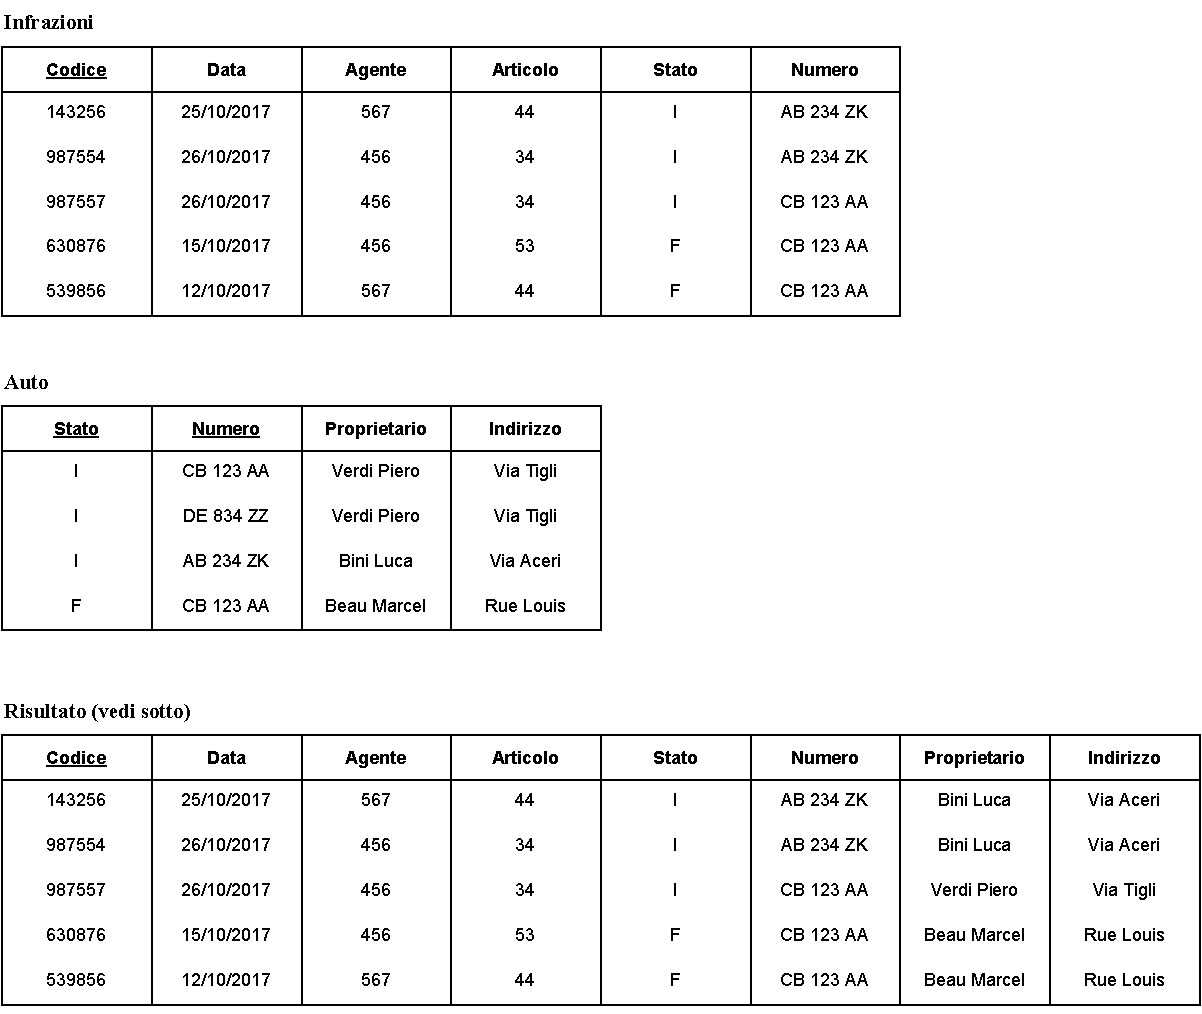
\includegraphics[width=\textwidth]{img/join_naturale2.pdf}
	\end{figure}
	
	\noindent
	Il risultato è ottenuto con la seguente operazione:
	
	\begin{equation*}
		\textsf{Infrazioni} \Join \textsf{Auto}
	\end{equation*}

	\newpage
	
	\subsubsection{Join completi e incompleti}
	
	Nell'esempio 1 nel paragrafo del \emph{join naturale}, si può dire che ciascuna tupla di ciascuno degli operandi contribuisce almeno una tupla del risultato (in questo caso il \emph{join} viene detto \textcolor{Red3}{\textbf{\underline{completo}}}): per ogni tupla $t_{1}$ di $r_{1}$, esiste una tupla $t$ in $r_{1} \Join r_{2}$ tale che $t\left[X_{1}\right] = t_{1}$ (e analogamente per $r_{2}$).
	
	L'esempio 1 a fine paragrafo, mostra un \emph{join} in cui alcune tuple degli operandi, in particolare la prima di $r_{1}$ e la seconda di $r_{2}$, non contribuiscono al risultato, perché l'altra relazione non contiene tuple con gli stessi valori sull'attributo comune. In questo caso il \emph{join} viene detto \textcolor{Red3}{\textbf{\underline{dangling}}}, ovvero \textbf{\emph{dondolante}}.
	
	Infine, come caso limite, è ovviamente possibile che nessuna delle tuple degli operandi sia combinabile, e allora il risultato del \emph{join} è la \textcolor{Red3}{\textbf{\underline{relazione vuota}}} (esempio 2 a fine paragrafo). All'estremo opposto, è possibile che ciascuna delle tuple di ciascuno degli operandi sia combinabile con tutte dell'altro, come mostrato nell'ultimo esempio del paragrafo, e in questo caso il risultato ha un numero di tuple pari al prodotto delle cardinalità degli operandi e cioè $|r_{1}| \times |r_{2}|$ (dove $|r|$ indica la cardinalità della relazione $r$).\newline
	
	\noindent
	Alcune osservazioni finali:
	\begin{itemize}
		\item Se il \emph{join} di $r_{1}$ e $r_{2}$ è completo, allora contiene almeno un numero di tuple pari al massimo fra $|r_{1}|$ e $|r_{2}|$;
		
		\item Se $X_{1} \cap X_{2}$ contiene una chiave per $r_{2}$, allora il \emph{join} di $r_{1}\left(X_{1}\right)$ e $r_{2}\left(X_{2}\right)$ contiene al più $|r_{1}|$ tuple;
		
		\item Se $X_{1} \cap X_{2}$ coincide con una chiave per $r_{2}$ e sussiste il vincolo di riferimento fra $X_{1} \cap X_{2}$ in $r_{1}$ e la chiave di $r_{2}$, allora il \emph{join} di $r_{1}\left(X_{1}\right)$ e $r_{2}\left(X_{2}\right)$ contiene esattamente $|r_{1}|$ tuple.
	\end{itemize}\newpage

	\noindent
	\textcolor{Green4}{\textbf{\emph{Esempio 1}}}
	
	\begin{figure}[!htp]
		\centering
		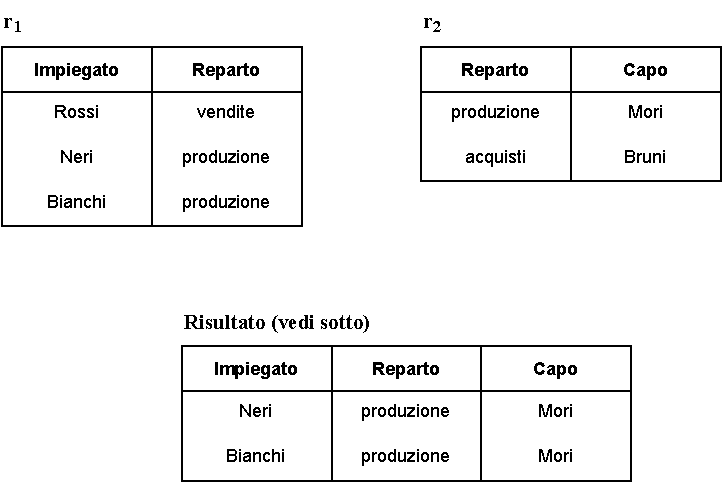
\includegraphics[width=0.9\textwidth]{img/join_dangling.pdf}
	\end{figure}
	
	\noindent
	Il risultato è ottenuto con la seguente operazione:
	\begin{equation*}
		r_{1} \Join r_{2}
	\end{equation*}
	
	\noindent
	\textcolor{Green4}{\textbf{\emph{Esempio 2}}}
	
	\begin{figure}[!htp]
		\centering
		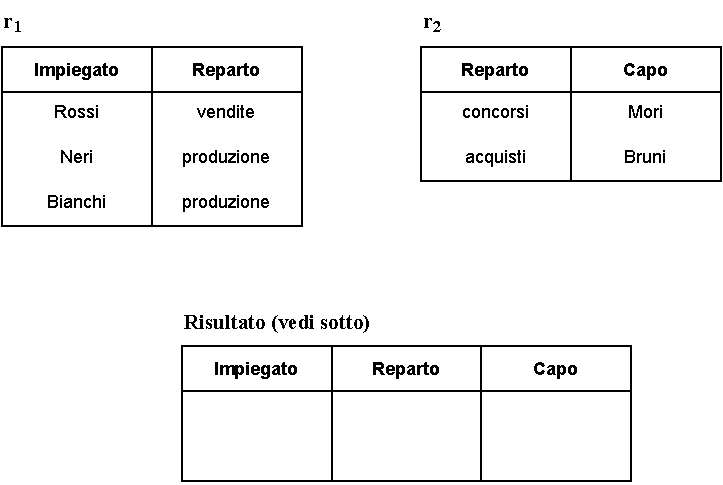
\includegraphics[width=0.9\textwidth]{img/join_vuoto.pdf}
	\end{figure}
	
	\noindent
	Il risultato è ottenuto con la seguente operazione:
	\begin{equation*}
		r_{1} \Join r_{2}
	\end{equation*}

	\newpage

	\noindent
	\textcolor{Green4}{\textbf{\emph{Esempio 3}}}

	\begin{figure}[!htp]
		\centering
		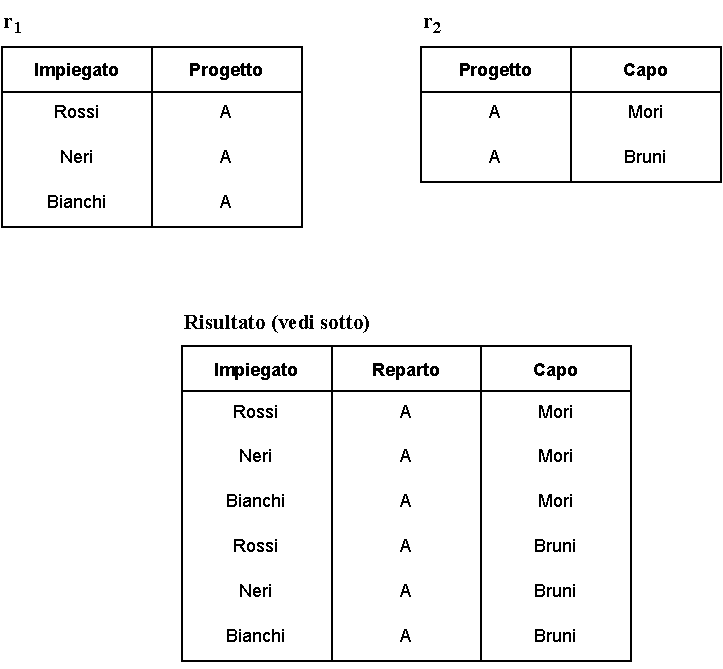
\includegraphics[width=0.9\textwidth]{img/join_massimo.pdf}
	\end{figure}
	
	\noindent
	Il risultato è ottenuto con la seguente operazione:
	\begin{equation*}
		r_{1} \Join r_{2}
	\end{equation*}\newpage

	\subsubsection{Theta-join ed equi-join}\label{theta-join}
	
	Osservando l'esempio 1 a fine paragrafo, è possibile notare come un prodotto cartesiano ha di solito ben poca utilità, in quanto concatena tuple non necessariamente correlate dal punto di vista semantico. Infatti, il \textbf{prodotto cartesiano viene spesso seguito da una selezione}, la quale centra l'attenzione su tuple correlate secondo le esigenze.\newline
	\textcolor{Green4}{\textbf{Per esempio}}, nell'esempio 2 a fine paragrafo, sulle relazione \textsf{Impiegati} e \textsf{Progetti} ha senso definire un prodotto cartesiano seguito dalla selezione che mantiene solo le tuple con valori uguali sull'attributo \textsf{\emph{Progetto}} di \textsf{Impiegati} e su \textsf{\emph{Codice}} di \textsf{Progetti}.
	
	Per questo motivo, viene definito un operatore derivato (cioè per mezzo di altri operatori), chiamato \textcolor{Red3}{\textbf{\underline{theta-join}}}. Esso è considerato come un \textbf{prodotto cartesiano seguito da una selezione}, nel modo seguente:
	\begin{equation*}
		r_{1} \underset{F}{\Join} r_{2} = \sigma_{F}\left(r_{1} \Join r_{2}\right)
	\end{equation*}
	\textbf{\underline{Attenzione!}} Gli schemi $r_{1}$ e $r_{2}$ devono essere \textbf{disgiunti}, cioè:
	\begin{equation*}
		r_{1} \cap r_{2} = \emptyset
	\end{equation*}
	\textcolor{Green4}{\textbf{Per esempio}}, nell'esempio 2 a fine paragrafo, la relazione può essere ottenuta per mezzo del \emph{theta-join}:
	\begin{equation*}
		\textsf{Impiegati } \underset{\textsf{\emph{Progetto}} = \textsf{\emph{Codice}}}{\Join} \textsf{Progetti}
	\end{equation*}
	Un \emph{theta-join} in cui la condizione di selezione $F$ sia una congiunzione di atomi di uguaglianza, con un attributo della prima relazione e uno della seconda, viene chiamato \textcolor{Red3}{\textbf{\underline{equi-join}}}. Quindi, la relazione scritta qua sopra è un \emph{equi-join}.
	
	Infine, il \textbf{join naturale è possibile simularlo} tramite la ridenominazione, l'\emph{equi-join} e la proiezione. Date due relazioni $r_{1}\left(ABC\right)$ e $r_{2}\left(BCD\right)$, il join naturale di $r_{1}$ e $r_{2}$ può essere espresso per mezzo degli altri operatori, in tre passi:
	\begin{enumerate}
		\item \textbf{Ridenominando} gli attributi così da ottenere relazioni su schemi disgiunti:
		\begin{equation*}
			\rho_{B'C' \leftarrow BC} \left(r_{2}\right)
		\end{equation*}
		
		\item Effettuando l'\textbf{\emph{equi-join}}, con condizioni di uguaglianza sugli attributi corrispondenti:
		\begin{equation*}
			r_{1} \underset{B = B' \land C = C'}{\Join} \rho_{B'C' \leftarrow BC} \left(r_{2}\right)
		\end{equation*}
		
		\item Concludendo con una \textbf{proiezione} che elimina gli attributi \dquotes{doppioni}, che presentano valori identici a quelli di altri attributi:
		\begin{equation*}
			\pi_{ABCD}\left(r_{1} \underset{B = B' \land C = C'}{\Join} \rho_{B'C' \leftarrow BC} \left(r_{2}\right)\right)
		\end{equation*}
	\end{enumerate}\newpage
	
	\noindent
	\textcolor{Green4}{\textbf{\emph{Esempio 1}}}
	
	\begin{figure}[!htp]
		\centering
		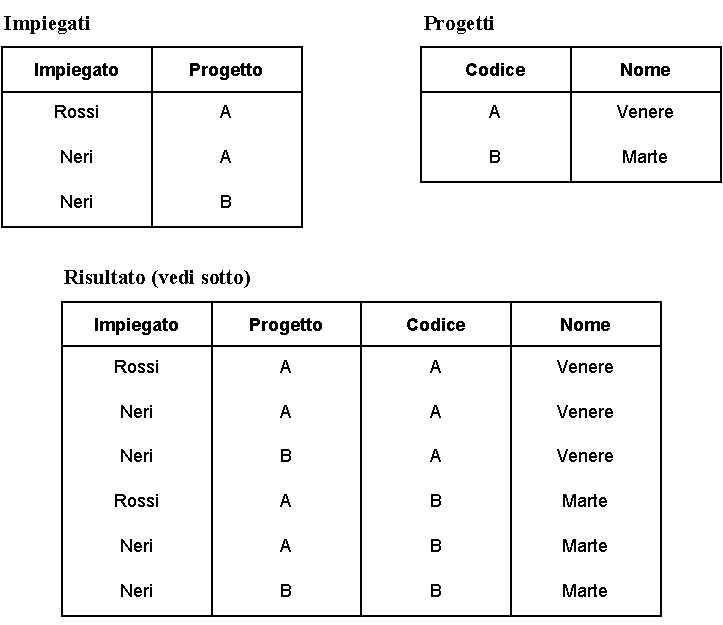
\includegraphics[width=0.9\textwidth]{img/join_theta.pdf}
	\end{figure}

	\noindent
	Il risultato è ottenuto con la seguente operazione:
	\begin{equation*}
		\textsf{Impiegati} \Join \textsf{Progetti}
	\end{equation*}\newpage

	\noindent
	\textcolor{Green4}{\textbf{\emph{Esempio 2}}}
	
	\begin{figure}[!htp]
		\centering
		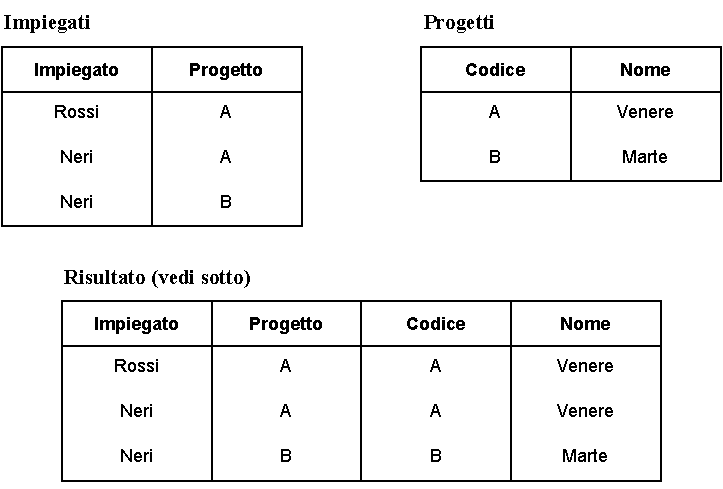
\includegraphics[width=0.9\textwidth]{img/join_theta2.pdf}
	\end{figure}
	
	\noindent
	Il risultato è ottenuto con la seguente operazione:
	\begin{equation*}
		\sigma_{\textsf{Progetto} = \textsf{Codice}}\left(\textsf{Impiegati} \Join \textsf{Progetti}\right)
	\end{equation*}\newpage
	
	\subsection{Algebra con valori nulli}
	
	È necessario introdurre la possibilità di avere dei valori nulli nell'algebra relazionale. Un \textcolor{Red3}{\textbf{\underline{valore nullo}}} (\emph{unknown}) viene rappresentato con il simbolo U e un \textbf{predicato prende tale valore quando almeno uno dei termini del confronto è \emph{sconosciuto}}. Considerando l'esempio a fine paragrafo, data la seguente selezione:
	\begin{equation*}
		\sigma_{\textsf{Eta} > 30}\left(\textsf{Persone}\right)
	\end{equation*}
	La prima tupla certamente appartiene al risultato (appartenenza \textbf{vera}), la seconda certamente non appartiene (appartenenza \textbf{falsa}), la terza forse appartiene e forse no (appartenenza \textbf{sconosciuta}).\newline
	
	\noindent
	Le \textbf{tabella di verità} dei connettivi \emph{not, and, or} tenendo conto del nuovo valore logico, si estendono nel seguente modo:
	\begin{table}[!htbp]
		\centering
		\begin{tabular}{@{} c | c @{}}
			\toprule
			\emph{not} & \phantom{\emph{not}} \\
			\midrule
			F & V \\
			U & U \\
			V & F \\
			\bottomrule
		\end{tabular}
		\hspace{3em}
		\begin{tabular}{@{} c | c c c @{}}
			\toprule
			\emph{and} & V & U & F \\
			\midrule
			V & V & U & F \\
			U & U & U & F \\
			F & F & F & F \\
			\bottomrule
		\end{tabular}
		\hspace{3em}
		\begin{tabular}{@{} c | c c c @{}}
			\toprule
			\emph{or} & V & U & F \\
			\midrule
			V & V & V & V \\
			U & V & U & U \\
			F & V & U & F \\
			\bottomrule
		\end{tabular}
	\end{table}
	Il valore nullo rappresenta un valore di verità intermedio tra vero e falso, e il significato dei tre connettivi in questo contesto diventa il seguente:
	\begin{itemize}
		\item Il \textbf{\emph{not}} è vero solo se il valore di partenza è falso;
		
		\item L'\textbf{\emph{and}} è vero solo se tutti i termini sono veri;
		
		\item L'\textbf{\emph{or}} è vero se almeno uno dei termini è vero.
	\end{itemize}
	Considerando ancora l'esempio a fine paragrafo, data la seguente espressione:
	\begin{equation*}
		\sigma_{\textsf{Eta} > 30}\left(\textsf{Persone}\right) \cup \sigma_{\textsf{Eta} \le 30}\left(\textsf{Persone}\right)
	\end{equation*}
	Logicamente si potrebbe pensare che il risultato sia esattamente la relazione \textsf{Persone}. Questo è \textbf{sbagliato} poiché la terza tupla, quella con il valore \textsf{NULL}, ha un'appartenenza sconosciuta a ciascuna sottoespressione e dunque anche all'unione. Questo discorso vale anche per la seguente espressione:
	\begin{equation*}
		\sigma_{\textsf{Eta} > 30 \lor \textsf{Eta} \le 30}\left(\textsf{Persone}\right)
	\end{equation*}
	In cui la disgiunzione viene valutata secondo la logica a tre valori.\newline
	
	\noindent
	Da questo problema nasce l'esigenza di esplicitare due nuove condizioni: \textcolor{Red3}{\textbf{IS NULL}} e \textcolor{Red3}{\textbf{IS NOT NULL}}. Il loro significato:
	\begin{itemize}
		\item $A$ \textsf{IS NULL} assume un valore vero su una tupla $t$ se il valore di $t$ su $A$ è nullo e falso (altrimenti) se esso è specificato;
		
		\item $A$ \textsf{IS NOT NULL} assume un valore vero su una tupla $t$ se il valore di $t$ su $A$ è specificato e falso (altrimenti) se esso è nullo;
	\end{itemize}
	Considerando l'esempio a fine paragrafo, data l'espressione:
	\begin{equation*}
		\sigma_{\textsf{Eta} > 30 \lor \textsf{Eta IS NULL}}\left(Persone\right)
	\end{equation*}
	Si ottiene le persone che hanno o potrebbero avere più di trent'anni (quindi età nota e maggiore di 30 oppure non nota). Invece, per ottenere tutte le tuple:
	\begin{equation*}
		\sigma_{\textsf{Eta} > 30 \lor \textsf{Eta} \le 30 \lor \textsf{Eta IS NULL}}\left(Persone\right)
	\end{equation*}\newline

	\noindent
	\textcolor{Green4}{\textbf{\emph{Esempio}}}
	\begin{figure}[!htp]
		\centering
		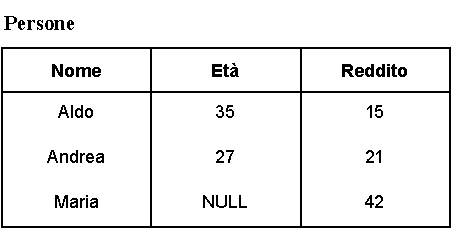
\includegraphics[width=.6\textwidth]{img/valori_nulli.pdf}
	\end{figure}\newpage

	\subsection{Ottimizzare ed equivalenza di espressioni algebriche}
	
	\subsubsection{Definizioni}
	
	Ogni espressione (\emph{query}) ricevuta dal DBMS è soggetta ad un processo di elaborazione. Esiste una parte software ad un livello più basso che implementa l'\textcolor{Red3}{\textbf{ottimizzatore}}. Esso ha l'obbiettivo di generare un'espressione equivalente all'originale ma con un costo minore. Per \textbf{costo} si intende la dimensione dei risultati intermedi.\newline
	
	\noindent
	Da questa necessità, si crea l'\textcolor{Red3}{\textbf{equivalenza delle espressioni algebriche}}, cioè espressioni fra loro equivalenti che producono quindi lo stesso risultato.\newline
	
	\noindent
	Esistono \textbf{due tipi} di equivalenza:
	\begin{itemize}
		\item \textbf{Equivalenza \underline{assoluta}}. Non viene esplicitato nessuno schema, quindi è completamente indipendente (assoluta).\newline
		Più formalmente:
		\begin{equation*}
			E_{1} \equiv E_{2} \text{ se } E_{1} \equiv_{\textbf{R}} E_{2} \text{ per ogni schema } \textbf{R}
		\end{equation*}
		Un \textcolor{Green4}{esempio}:
		\begin{equation*}
			\pi_{AB}\left(\sigma_{A>0}\left(R\right)\right) \equiv \sigma_{A>0}\left(\pi_{AB}\left(R\right)\right)
		\end{equation*}
		
		\item \textbf{Equivalenza \underline{dipendente dallo schema}}. Viene esplicitato lo schema e dunque l'equivalenza è vera se e solo se l'intersezione degli insiemi è uguale.\newline
		Più formalmente:
		\begin{equation*}
			E_{1} \equiv_{\textbf{R}} E_{2} \text{ se } E_{1}\left(\textbf{r}\right) = E_{2}\left(\textbf{r}\right) \text{ per ogni istanza } \textbf{r} \text{ di } \textbf{R}
		\end{equation*}
		Un \textcolor{Green4}{esempio}:
		\begin{equation*}
			\pi_{AB}\left(R_{1}\right) \Join \pi_{AC}\left(R_{2}\right) \equiv_{\textbf{R}} \pi_{ABC}\left(R_{1} \Join R_{2}\right)
		\end{equation*}
		L'equivalenza è valida se e solo se nello schema \textbf{R} l'intersezione fra gli insiemi di attributi di $R_{1}$ e $R_{2}$ è pari ad $A$.
	\end{itemize}\newpage
	
	\subsubsection{Trasformazioni di equivalenza}
	
	Nel conteso delle ottimizzazioni, vengono spesso utilizzate le \textcolor{Red3}{\textbf{trasformazioni di equivalenza}}, ovvero operazioni che \textbf{sostituiscono un'espressione con un'altra a essa equivalente}. In particolare, risultano interessanti le trasformazioni che riducono le dimensioni dei risultati intermedi e quelle che preparano un'espressione all'applicazione di una trasformazione che riduce le dimensioni dei risultati intermedi.
	\begin{enumerate}[label=\Roman*.]
		\item \textcolor{Red3}{\textbf{Atomizzazione delle selezioni}}: una selezione $\sigma$ congiuntiva\footnote{Ovvero due espressioni connesse da un and, or, not logico} può essere sostituita da una cascata di selezioni atomiche:
		\begin{equation*}
			\sigma_{F_{1} \land F_{2}}\left(E\right) \equiv \sigma_{F_{1}}\left(\sigma_{F_{2}}\left(E\right)\right)
		\end{equation*}
		In cui $E$ è una qualunque espressione.
	
		\item \textcolor{Red3}{\textbf{Idempotenza delle proiezioni}}: una proiezione $\pi$ può essere trasformata in una cascata di proiezioni che \dquotes{eliminano} i vari attributi in fasi successive:
		\begin{equation*}
			\pi_{X}\left(E\right) \equiv \pi_{X}\left(\pi_{XY}\left(E\right)\right)
		\end{equation*}
		Se $E$ è definita su un insieme di attributi che contiene $Y$ (oltre a $X$).
	
		\item \textcolor{Red3}{\textbf{\emph{Pushing selections down}} (\textbf{Anticipazione della selezione rispetto al join})}:
		\begin{equation*}
			\sigma_{F}\left(E_{1} \Join E_{2}\right) \equiv E_{1} \Join \sigma_{F}\left(E_{2}\right)
		\end{equation*}
		Se la condizione $F$ fa riferimento solo ad attributi nella sottoespressione $E_{2}$.
	
		\item \textcolor{Red3}{\textbf{\emph{Pushing projections down}} (\textbf{Anticipazione della proiezione rispetto al join})}: siano $E_{1}$ ed $E_{2}$ definite rispettivamente su $X_{1}$ e $X_{2}$. Allora, se $Y_{2} \subseteq X_{2}$ e $Y_{2} \supseteq \left(X_{1} \cap X_{2}\right)$, ovvero se gli attributi in $X_{2} - Y_{2}$ non sono coinvolti nel join, vale:
		\begin{equation*}
			\pi_{X_{1}Y_{2}}\left(E_{1} \Join E_{2}\right) \equiv E_{1} \Join \pi_{Y_{2}}\left(E_{2}\right)
		\end{equation*}
		Combinando questa regola con quella della idempotenza delle proiezioni, si può ottenere:
		\begin{equation*}
			\pi_{Y}\left(E_{1} \underset{F}{\Join} E_{2}\right) \equiv \pi_{Y}\left(\pi_{Y_{1}}\left(E_{1}\right) \underset{F}{\Join} \pi_{Y_{2}}\left(E_{2}\right)\right)
		\end{equation*}
		Si indica con $X_{1}$ e $X_{2}$ gli attributi di $E_{1}$ ed $E_{2}$ rispettivamente, con $J_{1}$ e $J_{2}$ i rispettivi sottoinsiemi coinvolti nella condizione $F$ di join:
		\begin{gather*}
			Y_{1} = \left(X_{1} \cap Y\right) \cup J_{1} \\
			Y_{2} = \left(X_{2} \cap Y\right) \cup J_{2} \\
		\end{gather*}
		In altre parole, è possibile \textbf{eliminare subito da ciascuna relazione gli attributi che non compaiono nel risultato finale e non sono coinvolti nel join}.
	
		\item \textcolor{Red3}{\textbf{Inglobamento di una selezione in un prodotto cartesiano a formare un join}}:
		\begin{equation*}
			\sigma_{F}\left(E_{1} \Join E_{2}\right) \equiv E_{1} \underset{F}{\Join} E_{2}
		\end{equation*}
		Indicando $X_{1}$ e $X_{2}$ i rispettivi attributi di $E_{1}, E_{2}$, allora $X_{1} \cap X_{2} = \emptyset$.
	\end{enumerate}
	Queste trasformate sono quelle più importanti.\newline
	
	\noindent
	Esistono altre trasformate non meno importanti ma di minore rilievo rispetto alle prime che sono considerate fondamentali.\footnote{\textbf{All'esame non verranno chieste le trasformate minori!}}
	\begin{enumerate}[label=\Roman*.]
		\setcounter{enumi}{5}
		\item \textbf{Distributività della selezione rispetto all'unione}:
		\begin{equation*}
			\sigma_{F}\left(E_{1} \cup E_{2}\right) \equiv \sigma_{F}\left(E_{1}\right) \cup \sigma_{F}\left(E_{2}\right)
		\end{equation*}
		
		\item \textbf{Distributività della selezione rispetto alla differenza}:
		\begin{equation*}
			\sigma_{F}\left(E_{1} - E_{2}\right) \equiv \sigma_{F}\left(E_{1}\right) - \sigma_{F}\left(E_{2}\right)
		\end{equation*}
		
		\item \textbf{Distributività della proiezione rispetto all'unione}:
		\begin{equation*}
			\pi_{X}\left(E_{1} \cup E_{2}\right) \equiv \pi_{X}\left(E_{1}\right) \cup \pi_{X}\left(E_{2}\right)
		\end{equation*}
	\end{enumerate}\:\newline
	
	\noindent
	Un altro gruppo minore di trasformate è quello basato sull'interazione fra gli operatori insiemistici e le selezioni complesse:
	\begin{enumerate}[label=\Roman*.]
		\setcounter{enumi}{8}
		\item $%
		\sigma_{F_{1} \lor F_{2}}\left(R\right) \equiv \sigma_{F_{1}}\left(R\right) \cup \sigma_{F_{2}}\left(R\right)$
		
		\item $%
		\sigma_{F_{1} \land F_{2}}\left(R\right) \equiv \sigma_{F_{1}}\left(R\right) \cap \sigma_{F_{2}}\left(R\right) \equiv \sigma_{F_{1}}\left(R\right) \Join \sigma_{F_{2}}\left(R\right)$
		
		\item $%
		\sigma_{F_{1} \land \lnot F_{2}}\left(R\right) \equiv \sigma_{F_{1}}\left(R\right) - \sigma_{F_{2}}\left(R\right)$
	\end{enumerate}\:\newline
	
	\noindent
	Infine, la \textbf{proprietà distributiva del join rispetto all'unione}:
	\begin{enumerate}[label=\Roman*.]
		\setcounter{enumi}{11}
		\item $%
		E \Join\left( E_{1} \cup E_{2} \right) \equiv \left(E \Join E_{1}\right) \cup \left(E \Join E_{2}\right)$
	\end{enumerate}\newpage
	
	\noindent
	\textcolor{Green4}{\textbf{\emph{Esempio}}}\newline
	
	\noindent
	Si vede un esempio per chiarire le trasformazioni più importanti. Data la seguente base di dati:
	\begin{figure}[!htp]
		\centering
		\includegraphics[width=\textwidth]{img/equivalenza_espressioni_algebriche.pdf}
		\label{Trasformazioni di equivalenza - Tabella}
	\end{figure}
	
	\noindent
	Si vuole trovare il numero di matricola dei capi di impiegati con meno di trenta anni. Immediatamente si potrebbe pensare di eseguire un join sulle due tabelle, specificare la condizione di selezione e infine proiettare l'unica colonna d'interesse:
	\begin{equation*}
		\pi_{\textsf{Capo}}\left(\sigma_{\textsf{Impiegato} = \textsf{Matricola} \land \textsf{Età} < 30} \left(\textsf{Impiegati} \Join \textsf{Supervisione}\right)\right)
	\end{equation*}
	È evidente che l'espressione risulta qualitativamente bassa poiché per calcolare pochi valori, in questo caso uno, viene effettuato un prodotto cartesiano che produce un risultato notevole. Quindi, si esegue l'ottimizzazione:
	\begin{enumerate}
		\item (Regola 1) Atomizzazione delle selezioni. Si elimina la coniugazione logica and:
		\begin{equation*}
			\pi_{\textsf{Capo}}\left(\sigma_{\textsf{Impiegato} = \textsf{Matricola}} \left(\sigma_{\textsf{Età} < 30} \left(\textsf{Impiegati} \Join \textsf{Supervisione}\right)\right)\right)
		\end{equation*}
	
		\item (Regola 3) Anticipazione della selezione rispetto al join e (Regola 5) inglobamento di una selezione in un prodotto cartesiano a formare un join. Si fonde la prima selezione ($\sigma_{\textsf{Impiegato} = \textsf{Matricola}}$) con il prodotto cartesiano formando un join con condizione e successivamente si anticipa la seconda selezione ($\sigma_{\textsf{Età} < 30}$) rispetto al join:
		\begin{equation*}
			\pi_{\textsf{Capo}}\left(
			\sigma_{\textsf{Età} < 30}\left(\textsf{Impiegati}\right) \underset{\textsf{Impiegato} = \textsf{Matricola}}{\Join} \textsf{Supervisione}
			\right)
		\end{equation*}
		
		\item (Regola 4) Anticipazione della proiezione rispetto al join. Si elimina dal primo argomento del join anche gli attributi non necessari:
		\begin{equation*}
			\pi_{\textsf{Capo}}\left(
			\pi_{\textsf{Matricola}}\left(\sigma_{\textsf{Età} < 30}\left(\textsf{Impiegati}\right)\right)
			\underset{\textsf{Impiegato} = \textsf{Matricola}}{\Join}
			\textsf{Supervisione}
			\right)
		\end{equation*}
	\end{enumerate}\newpage

	\section{Calcolo relazionale}
	
	Il \textcolor{Red3}{\underline{\textbf{calcolo relazionale}}} fa riferimento ad una famiglia di linguaggi di interrogazione, basati sul calcolo dei predicati del primo ordine, che hanno la caratteristica di essere \textbf{dichiarativi}, cioè di \textbf{specificare le proprietà del risultato delle interrogazioni, anziché la procedura seguita per generarlo}.
	
	Al contrario l'algebra relazionale è un \textbf{linguaggio procedurale} poiché le sue espressioni specificano passo passo la costruzione del risultato.\newline
	
	\noindent
	Esistono diversi \textbf{tipi} di calcolo relazionale:
	\begin{itemize}
		\item \textbf{Calcolo relazione su domini}. Presenta in modo naturale le caratteristiche originali dei linguaggi del calcolo relazionale.
		
		\item \textbf{Calcolo su tuple con dichiarazioni di range}. Metodo adottato durante questo corso, costituisce la base per molti costrutti disponibili per le interrogazioni nel linguaggio SQL.
	\end{itemize}
	Prima di presentare le varie caratteristiche, si tiene a precisare che rispetto al modello relazionale (paragrafo~\ref{Il modello Entità-Relazione (E-R)}), il calcolo su tuple con dichiarazioni di range utilizza una \textbf{notazione non posizionale}.\newpage
	
	\subsection{Calcolo su tuple con dichiarazioni di range}
	
	Il \textcolor{Red3}{\textbf{\underline{calcolo su tuple con dichiarazioni di range}}} presenta la seguente forma:
	\begin{equation*}
		\left\{T \: | \: L \: | \: f\right\}
	\end{equation*}
	In cui le variabili hanno diversi significati:
	\begin{itemize}
		\item La variabile $\boldsymbol{T}$ indica la \textbf{\emph{target list}}, ovvero la lista degli obbiettivi dell'interrogazione. I suoi elementi hanno la seguente forma $Y: x.Z$ con $x$ variabile e $Y$ e $Z$ sequenze di attributi (di pari lunghezza). Chiaramente, gli attributi in $Z$ devono comparire nello schema della relazione che costituisce il \emph{range} di $x$.\newline
		Una notazione alternativa per abbreviare $X: x.X$ è $x.*$;
		
		\item La variabile $\boldsymbol{L}$ indica la \textbf{\emph{range list}}, ovvero la lista contenente le variabili libere della formula $f$ con i relativi \emph{range}. I suoi elementi hanno la seguente forma $x\left(R\right)$ con $x$ variabile e $R$ nome di relazione;
		
		\item La variabile $\boldsymbol{f}$ indica una \textbf{formula}, la quale può essere di tre tipi:
		\begin{itemize}
			\item Formula con atomi del tipo:
			\begin{itemize}
				\item $x.A\theta c$, si confronta il valore di $x$ sull'attributo $A$ con la costante $c$;
				\item $x_{1}.A_{1}\theta x_{2}.A_{2}$, si confronta il valore di $x_{1}$ su $A_{1}$ con quello di $x_{2}$ su $A_{2}$.
			\end{itemize}
			
			\item Formula con connettivi ($\land, \lor, \lnot$);
			
			\item Formula con quantificatori che associano i range alle relative variabili:
			\begin{equation*}
				\exists x\left(R\right)\left(f\right) \hspace{2em} \forall x\left(R\right)\left(f\right)
			\end{equation*}
			Intuitivamente, $\exists x\left(R\right)\left(f\right)$ significa \dquotes{esiste nella relazione $R$ una tupla $x$ che soddisfa la formula $f$}.
		\end{itemize}
	\end{itemize}\newpage
	
	\subsection{Unione, intersezione e differenza}
	
	Purtroppo, il calcolo su tuple con dichiarazioni di range non permette di esprimere tutte le interrogazioni che possono essere formulate in algebra relazionale.\newline
	
	\noindent
	In particolare, le interrogazioni i cui risultati possono provenire indifferentemente da due o più relazioni (in algebra si realizza con un unione) non possono essere espresse in questa versione del calcolo.\newline
	
	\noindent
	Infatti, i risultati sono costituiti a partire da tutte le variabili libere, i cui range sono definiti nella target list, e ogni variabile ha come range una sola relazione.\newline
	
	\noindent
	Per esempio, si consideri un'unione di due relazioni sugli stessi attributi: $R_{1}\left(AB\right)$ e $R_{2}\left(AB\right)$. Se l'espressione avesse due variabili libere, allora ogni tupla del risultato dovrebbe corrispondere a una tupla di ciascuna delle relazioni, il che non è necessario, poiché l'unione richiede alle tuple nel risultato di comparire in almeno uno degli operandi, non necessariamente in entrambi. Viceversa, se l'espressione avesse una sola variabile libera, questa dovrebbe far riferimento a una sola delle relazioni, senza acquisire tuple dell'altra per il risultato.\newline
	
	\noindent
	Nonostante l'\textbf{operatore di unione non sia rappresentabile}, gli operatori di intersezione e differenza risultato esprimibili:
	\begin{itemize}
		\item L'\textbf{intersezione} richiede che le tuple siano in entrambi gli operandi, ovvero richiede l'esistenza di una tupla uguale nell'altra relazione. Per esempio:
		\begin{equation*}
			\pi_{BC}\left(R_{1}\right) \cap \pi_{BC}\left(R_{2}\right)
		\end{equation*}
		Si esprime come:
		\begin{equation*}
			\left\{x_{1}.BC \hspace{1em} |
			\hspace{1em} x_{1}\left(R_{1}\right) \hspace{1em} |
			\hspace{1em} \exists x_{2}\left(R_{2}\right)\left(x_{1}.B = x_{2}.B \land x_{1}.C = x_{2}.C\right)\right\}
		\end{equation*}
	
		\item La \textbf{differenza} produce le tuple di un operando non contenute nell'altro e può essere specificata richiedendo le tuple del minuendo che non compaiono nel sottraendo. Per esempio:
		\begin{equation*}
			\pi_{BC}\left(R_{1}\right) - \pi_{BC}\left(R_{2}\right)
		\end{equation*}
		Si esprime come:
		\begin{equation*}
			\left\{x_{1}.BC \hspace{1em} |
			\hspace{1em} x_{1}\left(R_{1}\right) \hspace{1em} |
			\hspace{1em} \lnot\exists x_{2}\left(R_{2}\right)\left(x_{1}.B = x_{2}.B \land x_{1}.C = x_{2}.C\right)\right\}
		\end{equation*}
	\end{itemize}\newpage
	
	\subsection[Esempi]{\textcolor{Green4}{Esempi}}
	
	Tutte le interrogazioni che verranno affrontate riguardano la seguente basi di dati (già vista nei precedenti paragrafi~\ref{Trasformazioni di equivalenza - Tabella}):
	\begin{figure}[!htp]
		\centering
		\includegraphics[width=\textwidth]{img/equivalenza_espressioni_algebriche.pdf}
	\end{figure}

	\noindent
	La prima interrogazione è la seguente:
	\begin{enumerate}
		\item \emph{Si richiede la matricola, il nome, l'età e lo stipendio degli impiegati che guadagnano più di 40 mila euro}:
		\begin{equation*}
			\left\{
			i.* \hspace{1em} | \hspace{1em}
			i\left(\textsf{Impiegati}\right) \hspace{1em} | \hspace{1em}
			i.\textsf{Stipendio} > 40
			\right\}
		\end{equation*}
	\end{enumerate}
	Per produrre meno risultati è sufficiente modificare la \emph{target list}:
	\begin{enumerate}
		\setcounter{enumi}{1}
		\item \emph{Si richiede la matricola, il nome e l'età degli impiegati che guadagnano più di 40 mila euro}:
		\begin{equation*}
			\left\{
			i.\left(\textsf{Matricola, Nome, Età}\right) \hspace{1em} | \hspace{1em}
			i\left(\textsf{Impiegati}\right) \hspace{1em} | \hspace{1em}
			i.\textsf{Stipendio} > 40
			\right\}
		\end{equation*}
	\end{enumerate}
	Per eseguire interrogazioni che coinvolgono più relazioni, si modifica la \emph{range list} usando più variabili. Si noti la prima condizione atomica che corrisponde a quella del join (e l'altra per la selezione):
	\begin{enumerate}
		\setcounter{enumi}{2}
		\item \emph{Trovare le matricole dei capi degli impiegati che guadagnano più di 40 mila euro}:
		\begin{gather*}
			\left\{
			s.\left(\textsf{Capo}\right) \hspace{1em} | \hspace{1em}
			i\left(\textsf{Impiegati}\right), s\left(\textsf{Supervisione}\right) \hspace{1em} | \hspace{1em} \right. \\
			\left. i.\textsf{Matricola} = s.\textsf{Impiegato} \land i.\textsf{Stipendio} > 40
			\right\}
		\end{gather*}
	\end{enumerate}
	Nel caso di join di una relazione con se stessa si ha più variabili aventi la stessa relazione come range:
	\begin{enumerate}
		\setcounter{enumi}{3}
		\item \emph{Trovare il nome e stipendio dei capi degli impiegati che guadagnano più di 40 mila euro}:
		\begin{gather*}
			\left\{
			\textsf{NomeC, StipC}: i'.\left(\textsf{Nome, Stipendio}\right) \hspace{1em} | \hspace{1em} \right. \\
			i'\left(\textsf{Impiegati}\right), s\left(\textsf{Supervisione}\right), i\left(\textsf{Impiegati}\right) \hspace{1em} | \hspace{1em} \\
			\left. i'.\textsf{Matricola} = s.\textsf{Capo} \land s.\textsf{Impiegato} = i.\textsf{Matricola} \land i.\textsf{Stipendio} > 40
			\right\}
		\end{gather*}
	
		\item \emph{Trovare gli impiegati che guadagnano più del rispettivo capo, mostrando matricola, nome e stipendio di ciascuno di essi e del capo}:
		\begin{gather*}
			\left\{
			i.\left(\textsf{Nome, Matr, Stip}\right), \textsf{NomeC, MatrC, StipC}: i'.\left(\textsf{Nome, Matr, Stip}\right) \hspace{1em} | \hspace{1em} \right. \\
			i\left(\textsf{Impiegati}\right), s\left(\textsf{Supervisione}\right), i'\left(\textsf{Impiegati}\right) \hspace{1em} | \hspace{1em} \\
			\left. i.\textsf{Matr} = s.\textsf{Impiegato} \land s.\textsf{Capo} = i'.\textsf{Matr} \land i.\textsf{Stipendio} > i'.\textsf{Stipendio}
			\right\}
		\end{gather*}
	\end{enumerate}
	Le interrogazioni con i quantificatori ($\exists, \forall$) mostrano appieno la maggiore sinteticità e praticità del calcolo su tuple con dichiarazioni di range:
	\begin{enumerate}
		\setcounter{enumi}{5}
		\item \emph{Trovare la matricola e il nome dei capi i cui impiegati guadagnano tutti più di 40 mila}:
		\begin{itemize}
			\item Quantificatore universale:
			\begin{gather*}
				\left\{
				i.\left(\textsf{Matricola, Nome}\right) \hspace{1em} | \hspace{1em}
				i\left(\textsf{Impiegati}\right), s\left(\textsf{Supervisione}\right) \hspace{1em} | \hspace{1em} \right. \\
				i.\textsf{Matr} = s.\textsf{Capo} \land \forall i'\left(\textsf{Impiegati}\right) \left(\forall s'\left(\textsf{Supervisione}\right) \right. \\
				\left.\left. \left(\lnot\left(s.\textsf{Capo} = s'.\textsf{Capo} \land s'.\textsf{Impiegato} = i'.\textsf{Matr}\right) \lor i'.\textsf{Stipendio} > 40\right)\right)
				\right\}
			\end{gather*}
		
			\item Quantificatore esistenziale:
			\begin{gather*}
				\left\{
				i.\left(\textsf{Matricola, Nome}\right) \hspace{1em} | \hspace{1em}
				i\left(\textsf{Impiegati}\right), s\left(\textsf{Supervisione}\right) \hspace{1em} | \hspace{1em} \right. \\
				i.\textsf{Matr} = s.\textsf{Capo} \land \lnot \left(\exists i'\left(\textsf{Impiegati}\right) \left(\exists s'\left(\textsf{Supervisione}\right) \right.\right. \\
				\left.\left.\left. \left(s.\textsf{Capo} = s'.\textsf{Capo} \land s'.\textsf{Impiegato} = i'.\textsf{Matr} \land i'.\textsf{Stipendio} \le 40\right)\right)\right)
				\right\}
			\end{gather*}
		\end{itemize}
	\end{enumerate}\newpage

	\subsection{Esercizi}
	
	\subsubsection{Aula, insegnamento, docente e lezione}
	
	\textcolor{Red3}{\textbf{\underline{Testo}}}\newline
	
	\noindent
	Dato il seguente schema relazionale:
	\begin{itemize}
		\item \textbf{AULA}(\underline{NomeAula}, Capienza, Edificio);
		\item \textbf{INSEGNAMENTO}(\underline{NomeIns, AnnoAcc}, Docente);
		\item \textbf{DOCENTE}(\underline{Matricola}, Nome, Cognome, Età, Ruolo: \{ordinario, associato, ricercatore, esterno\});
		\item \textbf{LEZIONE}(\underline{NomeIns, AnnoAcc, NomeAula, Giorno, Semestre, OraInizio}, OraFine).
	\end{itemize}
	Si calcoli:
	\begin{enumerate}
		\item Trovare il nome e la capienza delle aule dove nel 2° semestre 2015/2016 il venerdì non si sono svolte lezioni.
		\item Trovare i docenti che nel 1° semestre 2016/2017 hanno svolto almeno una lezione di durata maggiore di 180 minuti, riportando nel risultato il nome e il cognome del docente insieme alla durata della lezione (durata in minuti $=$ (\underline{OraFine} $-$ OraInizio)).
		\item Trovare per ogni lezione del 1° semestre 2016/2017 che si svolge il martedì prima delle 17.00 in aula A, la lezione immediatamente successiva nella stessa aula, riportando nel risultato per la prima lezione il nome dell’insegnamento, l’ora di inizio e l’ora di fine e per la lezione successiva solo il nome dell’insegnamento.
	\end{enumerate}\newpage
	
	\noindent
	\textcolor{Green4}{\textbf{\underline{Soluzione 1}}}\newline
	
	\noindent
	\emph{Trovare il nome e la capienza delle aule dove nel 2° semestre 2015/2016 il venerdì non si sono svolte lezioni.}\newline

	\noindent
	La soluzione è la seguente:
	\begin{gather*}
		Q = \left\{
		\text{Nome, Capienza}: A\left(\text{NomeAula, Capienza}\right) \hspace{1em} | \hspace{1em} A\left(\text{Aula}\right) \hspace{1em} | \hspace{1em} \right. \\
		\lnot\exists L\left(\text{Lezione}\right)\left(A\left(\text{NomeAula}\right) = L\left(\text{NomeAula}\right) \land L\left(\text{AnnoAcc}\right) = "2015/2016" \land \right. \\
		\left. \left.\left. L\left(\text{Semestre}\right) = "2^{\mathrm{o}}" \land L\left(\text{Giorno}\right) = "\text{Venerdì}"\right) 
		\right)\right\}
	\end{gather*}
	Il nome e la capienza delle aule si trovano nella tabella Aula, per cui nella \emph{target list} andranno i suoi due campi e basta.\newline
	
	\noindent
	Nella \emph{range list} è sufficiente l'aula, nonostante nella tabella lezione ci siano alcuni dati importanti.\newline
	
	\noindent
	Nel campo formula ci sono alcune condizioni. Per manifestare la negazione è necessario l'operatore logico \emph{not}. Esso deve operare su un campo presente nella tabella Lezione, ma allo stesso tempo deve avere le caratteristiche richieste dal risultato. Quindi, si scrive che non esiste una $L$ appartenente alla tabella Lezione tale per cui essa abbia:
	\begin{itemize}
		\item Il nome dell'aula (chiave) uguale sia nella tabella Aula che Lezione;
		\item L'anno accademico (tabella Lezione) uguale al valore $2015/2016$;
		\item Il semestre (tabella Lezione) uguale al valore $2^{\mathrm{o}}$;
		\item Il giorno (tabella Lezione) uguale al valore Venerdì.
	\end{itemize}
	Quindi, in questo caso si richiede una Lezione che non è presente nella tabella Aula, cioè che non si sia svolta. Tuttavia, oltre a non essersi svolta, deve in un anno, semestre e giorno preciso.\newpage
	
	\noindent
	\textcolor{Green4}{\textbf{\underline{Soluzione 2}}}\newline
	
	\noindent
	\emph{Trovare i docenti che nel 1° semestre 2016/2017 hanno svolto almeno una lezione di durata maggiore di 180 minuti, riportando nel risultato il nome e il cognome del docente insieme alla durata della lezione (durata in minuti $=$ (\underline{OraFine} $-$ OraInizio)).}\newline
	
	\noindent
	La soluzione è la seguente:
	\begin{gather*}
		Q = \left\{
		\text{Nome, Cognome}: D\left(\text{Nome, Cognome}\right), \right. \\
		\text{Durata Lezione}: L\left(\text{OraFine}\right) - L\left(\text{OraInizio}\right) \hspace{1em} | \hspace{1em} \\
		D\left(\text{Docente}\right), I\left(\text{Insegnamento}\right), L\left(\text{Lezione}\right) \hspace{1em} | \hspace{1em} \\
		D\left(\text{Matricola}\right) = I\left(\text{Docente}\right) \land I\left(\text{NomeIns}\right) = L\left(\text{NomeIns}\right) \land \\
		I\left(\text{AnnoAcc}\right) = L\left(\text{AnnoAcc}\right) \land L\left(\text{AnnoAcc}\right) = "2016/2017" \land L\left(\text{Semestre}\right) = 1^{\mathrm{o}} \land \\
		\left. \left. \left(L\left(\text{OraFine}\right) - L\left(\text{OraInizio}\right)\right) \ge 180
		\right)\right\}
	\end{gather*}
	Il risultato richiede il nome e il cognome del docente, quindi la \emph{target list} avrà tali campi e la durata. Quest'ultima sarà specificata eseguendo la differenza tra l'ora di fine e l'ora di inizio.\newline
	
	\noindent
	Nella \emph{range list} si specifica ovviamente la tabella del docente, dell'insegnamento e della lezione.\newline
	
	\noindent
	Nel campo formula ci sono alcune condizioni. È necessario collegare tutte le chiavi esterne, quindi le matricole del docente, il nome e l'anno accademico tra l'Insegnamento e la Lezione. Inoltre, le condizioni sul numero di semestre, anno accademico e durata delle lezioni, cioè ora di inizio e fine, sono specificate nella tabella Lezione. Quindi, le condizioni vengono espresse su di essa.\newpage
	
	\noindent
	\textcolor{Green4}{\textbf{\underline{Soluzione 3}}}\newline
	
	\noindent
	\emph{Trovare per ogni lezione del 1° semestre 2016/2017 che si svolge il martedì prima delle 17.00 in aula A, la lezione immediatamente successiva nella stessa aula, riportando nel risultato per la prima lezione il nome dell’insegnamento, l’ora di inizio e l’ora di fine e per la lezione successiva solo il nome dell’insegnamento.}\newline
	
	\noindent
	La soluzione è la seguente:
	\begin{gather*}
		Q = \left\{
		\text{Ins, Inizio, Fine}: L1.\left(\text{NomeIns, OraInizio, OraFine}\right), \right. \\
		\text{InsSuccessivo}: L2.\left(\text{NomeIns}\right) \hspace{1em} | \hspace{1em} L1\left(\text{LEZIONE}\right), L2\left(\text{LEZIONE}\right) \hspace{1em} | \hspace{1em} \\
		L1.\text{Semetre} = "1" \land L2.\text{Semestre} = "1" \land L1.\text{AnnoAcc} = "2016/2017" \land \\
		L2.\text{AnnoAcc} = "2016/2017" \land L1.\text{Giorno} = "\text{Martedì}" \land L2.\text{Giorno} = "\text{Martedì}" \land \\
		L1.\text{NomeAula} = "\text{A}" \land L2.\text{NomeAula} = "\text{A}" \land L1.\text{OraInizio} < 17:00 \land \\ L1.\text{OraInizio} < L2.\text{OraInizio} \land \lnot \exists L3\left(\text{LEZIONE}\right)\left( L3.\text{Semestre} = "1" \land \right. \\
		L3.\text{AnnoAcc} = "2016/2017" \land L3.\text{Giorno} = "\text{Martedì}" \land L3.\text{NomeAula} = "\text{A}" \land \\
		\left. L1.\text{OraInizio} < L3.\text{OraInizio} \land L3.\text{OraInizio} < L2.\text{OraInizio}
		\right)\left.
		\right\}
	\end{gather*}
	Il risultato richiede il nome, l'ora di inizio e l'ora di fine dell'insegnamento della prima lezione. Inoltre, anche il nome dell'insegnamento della lezione successiva alla prima. Quindi, nella \emph{target list} si aggiungono tali campi\newline
	
	\noindent
	Nella \emph{range list} si specificano due riferimenti diversi per la tabella LEZIONE poiché sono necessari per indicare due lezioni diverse. Entrambi si riferiscono alla tabella LEZIONE dato che in essa ci sono tutti i dati richiesti.\newline
	
	\noindent
	Nel campo formula ci sono alcune condizioni. Le prime condizioni sono necessarie per indicare che la lezione prima delle ore $17:00$ e quella successiva:
	\begin{itemize}
		\item Siano del primo semestre;
		\item Dell'anno accademico $2016/2017$;
		\item Si svolgano di martedì;
		\item La prima lezione si svolga prima delle ore $17:00$ (è sufficiente l'ora di inizio);
		\item La successiva (seconda) lezione si svolga dopo l'ora di inizio della prima.
	\end{itemize}
	Oltre a queste condizioni, è necessario specificare che la seconda lezione $L2$ sia la successiva di $L1$. Per farlo, è possibile utilizzare il quantificatore esistenziale per negare l'esistenza di una lezione tra la prima e la seconda. In questo modo, quest'ultima diventa la successiva. Quindi, le condizioni del semestre, anno accademico, giorno e aula sono le stesse. Al contrario, l'ora di inizio dovrà essere successiva alla prima lezione $L1$ e dovrà essere anche precedente alla seconda lezione $L2$. Negando l'esistenza di una lezione con queste condizioni, si ottiene la successione.\newpage
	
	\section{Tecnologie per le basi di dati}
	
	\subsection{Transazioni}
	
	Una \textcolor{Red3}{\textbf{transazione}} identifica un'unità elementare di lavoro svolta da un'applicazione, su cui si vogliono associare particolari \underline{proprietà} di \textbf{correttezza}, \textbf{robustezza} e \textbf{isolamento}.\newline
	
	\noindent
	Un sistema che mette a disposizione un meccanismo per la definizione e l'esecuzione di transazioni con le caratteristiche suddette viene detto \textbf{sistema transazionale}.\newline
	
	\noindent
	La \textbf{principale caratteristica} di una transazione è che essa, una volta eseguita, si è certi che non ci saranno esecuzioni parziali. Dunque, l'operazione andrà a buon fine, oppure fallirà senza modificare la base dati.
	
	\subsection{Transazioni in SQL}
	
	La \textbf{sintassi} di una transazione in SQL è la seguente:
	\begin{lstlisting}[language=SQL]
begin transaction
	<istruzione> | commit work | rollback work
end transaction
	\end{lstlisting}
	Dove al posto di:
	\begin{itemize}
		\item \textsf{Istruzione}, possono andare una serie di comandi da eseguire;
		\item \textsf{Commit work} (abbreviazione \textsf{commit}), la transazione va a buon fine al raggiungimento di tale operazione;
		\item \textsf{Rollback work} (abbreviazione \textsf{rollback}), la transazione non ha alcun effetto al raggiungimento di tale operazione.
	\end{itemize}
	Una \textbf{transazione} è \textbf{ben formattata} se rispetta le seguenti caratteristiche:
	\begin{enumerate}
		\item Inizia con un'istruzione \textsf{begin transaction};
		\item Termina con un'istruzione \textsf{end transaction};
		\item L'esecuzione incontra un \textsf{commit} o un \textsf{rollaback} e successivamente non esegue altri accessi alla base di dati.
	\end{enumerate}\newpage

	\noindent
	\textcolor{Green4}{\textbf{Esempio}} di transazione ben formata:
	\begin{lstlisting}[language=SQL]
begin transaction;
	update ContoCorrente
		set Saldo = Saldo + 10
		where NumConto = 12202;
	update ContoCorrente
		set Saldo = Saldo - 10
		where NumConto = 42177;
	select Saldo into A
		from ContoCorrente
		where NumConto = 42177;
	if A >= 0
		then commit work;
		else rollback work;
end transaction;
	\end{lstlisting}

	\longline
	
	\subsection{Proprietà acide delle transazioni}
	
	Una transazione possiede quattro \textcolor{Red3}{\textbf{proprietà acide}} (Atomicity Consistency Isolation Durability, ACID) che sono:
	\begin{itemize}
		\item \textbf{Atomicità} (\emph{Atomicity})
		\item \textbf{Consistenza} (\emph{Consistency})
		\item \textbf{Isolamento} (\emph{Isolation})
		\item \textbf{Persistenza} (\emph{Durability})
	\end{itemize}
	
	
	\subsubsection{Atomicità}
	
	L'\textcolor{Red3}{\textbf{atomicità}} rappresenta il fatto che una transazione è un'unità \textbf{indivisibile} di esecuzione. Quindi, o vengono resi visibili tutti gli effetti di una transazione, oppure essa non deve aver alcun effetto sulla base di dati (tutto o niente).\newline
	Per applicare questa proprietà, si implementano due implicazioni:
	\begin{itemize}
		\item \textbf{Transazione interrotta \underline{prima}} del \textsf{commit}, il sistema deve ricostruire la situazione esistente prima dell'esecuzione della transazione eliminando il lavoro eseguito fino a quel momento.
		\item \textbf{Transazione interrotta \underline{dopo}} il \textsf{commit}, il sistema deve assicurare che la transazione lasci la base di dati nel suo stato finale.
	\end{itemize}\newpage

	\subsubsection{Consistenza}
	
	La \textcolor{Red3}{\textbf{consistenza}} richiede che l'esecuzione della transazione non violi i vincoli di integrità definiti sulla base di dati. Nel caso di una violazione, il sistema interviene per annullare la transazione o per correggere la violazione del vincolo.\newline
	Il controllo della violazione può essere di due tipi:
	\begin{itemize}
		\item \textbf{Controllo della violazione \underline{immediata}}. I controlli vengono eseguiti durante l'esecuzione della transazione. Così facendo, è possibile rimuovere gli effetti della specifica istruzione di manipolazione dei dati che causa la violazione del vincolo, senza imporre un aborto delle transazioni.
		\item \textbf{Controllo della violazione \underline{differita}}. I controlli vengono eseguiti al termine dell'esecuzione della transazione, ovvero dopo il \textsf{commit}. Nel caso in cui ci sia una violazione, viene abortita l'intera transazione.
	\end{itemize}
	
	\subsubsection{Isolamento}
	
	L'\textcolor{Red3}{\textbf{isolamento}} richiede che l'esecuzione di una transazione sia indipendente dalla contemporanea esecuzione di altre transazioni.\newline
	Per applicare questa proprietà, si implementano due implicazioni:
	\begin{itemize}
		\item \textbf{Esecuzione concorrente} di un insieme di transazioni deve essere analogo al risultato che le stesse transazioni otterrebbero qualora ciascuna di esse fosse eseguita da sola.
		\item \textbf{Esecuzione indipendente}. L'esecuzione indipendente di ogni transazione evita che un eventuale \textsf{rollback} provochi un effetto domino generando una \textsf{rollback} anche nelle altre.
	\end{itemize}

	\subsubsection{Persistenza}
	
	La \textcolor{Red3}{\textbf{persistenza}} richiede che l'esecuzione di una transazione che ha eseguito il \textsf{commit} correttamente non venga più perso.\newline
	L'applicazione di questa proprietà garantisce gli effetti delle transazioni che, al momento di un eventuale guasto, abbiano già eseguito un \textsf{commit}.\newpage
	
	\subsection{Architettura di riferimento di un DBMS}
	
	Si lascia qui di seguito l'immagine di un'architettura di un DBMS. Non è necessario approfondire più di tanto tale argomento, ma è utile sapere della sua conoscenza. L'unica cosa \textbf{importante} da ricordare è \textbf{quali sono i moduli che contribuiscono a garantire le proprietà delle transizioni}:
	\begin{itemize}
		\item Gestore dei metodi d'accesso:
		\begin{itemize}
			\item Consistenza
		\end{itemize}
		
		\item Gestore dell'esecuzione concorrente:
		\begin{itemize}
			\item Atomicità
			\item Isolamento
		\end{itemize}
	
		\item Gestore dell'affidabilità
		\begin{itemize}
			\item Atomicità
			\item Persistenza
		\end{itemize}
	\end{itemize}
	
	\begin{figure}[!htp]
		\centering
		\includegraphics[width=\textwidth]{img/architettura_DBMS.pdf}
		\caption{Architettura generale di un DBMS.}
	\end{figure}\newpage
	
	\subsubsection{Gestore (ottimizzatore) delle interrogazioni}
	
	\begin{figure}[!htp]
		\centering
		\includegraphics[width=\textwidth]{img/gestore_interrogazioni.pdf}
		\caption{Gestore (ottimizzatore) delle interrogazioni.}
	\end{figure}

	\subsubsection{Gestore dei metodi d'accesso e dell'esecuzione concorrente}
	
	\begin{figure}[!htp]
		\centering
		\includegraphics[width=\textwidth]{img/gestore_metodi_accesso_e_esecuzione.pdf}
		\caption{Gestore dei metodi d'accesso e dell'esecuzione concorrente.}
	\end{figure}\newpage

	\subsubsection{Gestore dei metodi d'accesso e dell'affidabilità}
	
	\begin{figure}[!htp]
		\centering
		\includegraphics[width=\textwidth]{img/gestore_metodi_accesso_e_affidabilita.pdf}
		\caption{Gestore dei metodi d'accesso e dell'affidabilità.}
	\end{figure}

	\subsubsection{Gestore dell'affidabilità e del buffer}
	
	\begin{figure}[!htp]
		\centering
		\includegraphics[width=\textwidth]{img/gestore_affidabilita_e_buffer.pdf}
		\caption{Gestore dell'affidabilità e del buffer.}
	\end{figure}\newpage

	\section{Approfondimento gestore dell'affidabilità e del buffer}
	
	\subsection{Memoria secondaria}
	
	Le basi di dati hanno la necessità di \textbf{gestire dati in memoria secondaria per due motivi}:
	\begin{enumerate}
		\item La \textbf{dimensione della \underline{memoria primaria}} (e.g. RAM) \textbf{\underline{non è sufficiente}} per contenere interamente una base di dati;
		
		\item Le basi di dati hanno come \textbf{caratteristica fondamentale la \underline{persistenza}}. Essa è possibile \textbf{applicarla solo su una memoria} di massa (\textbf{secondaria}) sulla quale i dati non possono essere persi.
	\end{enumerate}
	Si elencano alcune \textbf{caratteristiche} delle memorie secondarie:
	\begin{itemize}
		\item Una memoria secondaria \textbf{\underline{non può essere utilizzata direttamente dai}} \textbf{\underline{programmi}}, ma prima è necessario un passaggio attraverso la memoria primaria;
		
		\item I \textbf{\underline{dati}} sono organizzati in \textbf{\underline{blocchi}} di dimensione fissa o variabile a seconda del sistema;
		
		\item Le \textbf{\underline{operazioni}} ammesse sono due: \textbf{\underline{lettura e scrittura}} di un blocco;
		
		\item Il tempo di lettura/scrittura di un blocco è molto più alto rispetto ad un accesso e ad un'elaborazione dei dati in memoria centrale (e.g. RAM). Quindi, solitamente si \textbf{\underline{conteggiano solo gli accessi alla memoria secondaria}}, quindi il numero di blocchi letti o scritti.
	\end{itemize}\newpage
	
	\subsection{Gestione del buffer}
	
	L'interazione tra la memoria centrale e la memoria secondaria è realizzata nel DBMS attraverso l'utilizzo di una \textbf{zona della memoria centrale} chiamata \textcolor{Red3}{\textbf{buffer}} e \textbf{condivisa con tutte le applicazioni}.\newline
	
	\noindent
	L'\underline{\textbf{obbiettivo}} del \emph{buffer} è quello di evitare di ripetere accessi multipli alla memoria secondaria per tutti quei dati che vengono utilizzati più volte in un tempo ravvicinato. La sua gestione è dunque fondamentale.\newline
	
	\noindent
	Un \emph{buffer} è \textbf{\underline{organizzato} in pagine di dimensione pari a un numero intero di blocchi}. Il \textbf{gestore del buffer} si occupa del \textbf{caricamento} e dello \textbf{scaricamento} (salvataggio) delle pagine dalla memoria centrale alla memoria di massa. Per semplicità, si può dire che ogni caricamento o salvataggio di pagina richiede un'operazione su memoria di massa (lettura o scrittura rispettivamente).\newline
	
	\noindent
	Quindi, le \underline{\textbf{operazioni}} sono:
	\begin{itemize}
		\item \textbf{Lettura}, lettura dal buffer se presente, altrimenti lettura fisica;
		\item \textbf{Scrittura}, gestore del buffer differisce la scrittura fisica se tale attesa è compatibile con la proprietà di affidabilità del sistema, ovvero se si è sicuri che l'operazione vada a buon fine.
	\end{itemize}
	La gestione del buffer segue il \textcolor{Red3}{\textbf{principio di località dei dati}}: i dati referenziati di recente hanno maggior probabilità di essere referenziati nuovamente nel futuro. Ne consegue che i buffer contengono le pagine sulle quali vengono fatte la maggior parte degli accessi. Inoltre, una \textbf{legge empirica} afferma che il $20\%$ dei dati è tipicamente acceduto dall'$80\%$ delle applicazioni.\newline
	
	\noindent
	Il \textbf{gestore del buffer} memorizza alcune \underline{\textbf{informazioni}}:
	\begin{itemize}
		\item Descrizione del contenuto corrente del buffer indicando per \emph{ogni} pagina:
		\begin{itemize}
			\item Il \textbf{file fisico}
			\item Il \textbf{numero di blocco}
		\end{itemize}

		\item Mantenimento di alcune variabili di stato:
		\begin{itemize}
			\item \textbf{Contatore} per indicare quanti programmi utilizzano la pagina
			\item \textbf{Bit di stato} per indicare se la pagina è stata modificata
		\end{itemize}
	\end{itemize}\newpage

	\subsection{Primitive per la gestione del buffer}
	
	\subsubsection{Primitiva \textsf{fix}}
	
	La primitiva \textcolor{Red3}{\textbf{\textsf{fix}}} viene utilizzata dalle transazioni per \textbf{richiedere l'accesso ad una pagina}. Essa restituisce al chiamante il riferimento (puntatore) alla pagina del buffer, in modo che esso possa accedere effettivamente ai dati. L'esecuzione della primitiva è realizzata nel modo seguente.
	\begin{enumerate}
		\item Viene \textbf{cercata la pagina tra quelle in memoria}. Se viene trovata, l'operazione si conclude e l'indirizzo della pagina (puntatore) viene restituito alla transazione richiedente;
		
		\item Se non viene trovata la pagina in memoria, viene \textbf{scelta una pagina dal buffer} cercando tra le pagine libere, ovvero con contatore pari a zero. La scelta viene fatta a seconda della strategia adottata, per esempio selezionando la pagina usata meno di recente (LRU, \emph{least recently used}), oppure selezionando quella caricata da più tempo (FIFO, \emph{first input first output}). Inoltre, nel caso in cui il bit di stato segnala che la pagina è stata modificata, essa viene aggiornata in memoria di massa (operazione di \emph{flush}). Infine, viene identificata la pagina da caricare nel buffer e successivamente avviene l'operazione di lettura.
		
		\item Se non esistono pagine libere, il gestore del buffer può scegliere due approcci differenti:
		\begin{enumerate}
			\item Approccio \textbf{\emph{steal}}, viene sottratta una pagina a un'altra transazione. La pagina sottratta viene chiamata vittima e viene scaricata in memoria di massa (operazione di \emph{flush}). Infine, vengono eseguite le operazioni di conversione di indirizzi e successivamente l'operazione di lettura.
			
			\item Approccio \textbf{\emph{non steal}}, la transazione viene sospesa, in attesa che si liberino pagine dal buffer. Quindi, essa entra in una coda di transazioni, la quale è mantenuta dal gestore del buffer. Nel momento in cui si libera una pagina, viene identificata, caricata nel buffer e successivamente avviene l'operazione di lettura.
		\end{enumerate}
	\end{enumerate}
	In ogni caso, \textbf{quando si effettua un accesso ad una pagina, viene incrementato il contatore relativo all'utilizzo della pagina}.\newpage
	
	\begin{figure}[!htp]
		\centering
		\includegraphics[width=\textwidth]{img/gestione_del_buffer-fix.pdf}
		\caption{Diagramma a blocchi della primitiva fix}
	\end{figure}
	
	\subsubsection{Primitiva \textsf{setDirty}}
	
	La primitiva \textcolor{Red3}{\textbf{\textsf{setDirty}}} indica al gestore del buffer che \textbf{una pagina è stata modificata}. Il suo effetto è la modifica del bit di stato relativo.
	
	\subsubsection{Primitiva \textsf{unfix}}
	
	La primitiva \textcolor{Red3}{\textbf{\textsf{unfix}}} indica al gestore del buffer che il modulo \textbf{chiamante ha terminato di usare la pagina}. Il suo effetto è decrementare il contatore di utilizzo della pagina.
	
	\subsubsection{Primitiva \textsf{force}}
	
	La primitiva \textcolor{Red3}{\textbf{\textsf{force}}} \textbf{trascrive} in memoria di massa, in modo sincrono, una \textbf{pagina del buffer}.\newpage
	
	\subsection{Gestore dell'affidabilità}
	
	Il \textcolor{Red3}{\textbf{controllo dell'affidabilità}} garantisce due \textbf{proprietà fondamentali} delle transazioni: atomicità e persistenza.
	\begin{itemize}
		\item \textbf{Atomicità}, garantire che le transazioni non vengano lasciate incomplete
		\item \textbf{Persistenza}, garantire che gli effetti di ciascuna transazione conclusa con un \emph{commit} siano mantenuti in modo permanente
	\end{itemize}
	Il gestore dell'affidabilità garantisce queste proprietà tramite il \textbf{log}, ovvero un archivio persistente su cui registra le varie azioni svolte dal DBMS.\newline
	
	\noindent
	L'\textbf{architettura} del controllore di affidabilità è descritta nella seguente immagine.
	\begin{figure}[!htp]
		\centering
		\includegraphics[width=\textwidth]{img/architettura_gestore_affidabilita.pdf}
		\caption{Architettura di un gestore dell'affidabilità.}
	\end{figure}
	
	\noindent
	Il controllore dell'affidabilità riceve richieste di accessi a pagine in lettura e scrittura, che passa al \emph{buffer manager}, e genera altre richieste di lettura e scrittura di pagine necessarie a garantire la robustezza e la resistenza ai guasti.\newline
	
	\noindent
	Inoltre, questa componente per eseguire il suo compito necessita di una \textbf{\underline{memoria}} \textbf{\underline{stabile}}, ovvero una memoria che risulti resistente ai guasti. Ovviamente, non esiste un dispositivo con tali caratteristiche, ma grazie ad alcuni meccanismi, è possibile rendere tale probabilità prossima allo zero.\newpage
	
	\subsubsection{Definizione log}
	
	Il \textcolor{Red3}{\textbf{log}} è un file sequenziale di cui è responsabile il controllore dell'affidabilità, scritto in memoria stabile e contenente informazione ridondante che \textbf{consente di ricostruire il contenuto della base di dati a seguito di guasti}. L'\textbf{ordine} di \textbf{salvataggio} delle varie transazioni è quello \textbf{temporale}.\newline
	
	\noindent
	Ogni salvataggio produce un \emph{record} nel file, il quale può essere di due \textbf{tipi}:
	\begin{enumerate}
		\item \textcolor{Red3}{\textbf{Record di transazione}}, identificano le \textbf{attività svolte da ciascuna transazione}. Quindi, ogni transazione inserisce nel log un record di \textsf{begin} (corrispondente al \textsf{start transaction}), vari record relativi alle azioni effettuate (corrispondente ad \textsf{insert}, \textsf{delete}, \textsf{update}) e un record di \textsf{commit} oppure di \textsf{abort} (corrispondente a \textsf{rollback}).
		
		\item \textcolor{Red3}{\textbf{Record di sistema}}, indicano l'\textbf{effettuazione di operazioni} specifiche del controllore dell'affidabilità che in totale sono due: \textbf{\emph{dump}} e \textbf{\emph{checkpoint}}.
	\end{enumerate}\newpage
	
	\subsubsection{Notazione dei record nel log}
	
	I \textbf{record che descrivono una transizione} vengono identificati nel seguente modo:
	\begin{itemize}
		\item I record:
		\begin{itemize}
			\item \textsf{begin} $\longrightarrow B\left(T\right)$
			\item \textsf{commit} $\longrightarrow C\left(T\right)$
			\item \textsf{abort} $\longrightarrow A\left(T\right)$
		\end{itemize}
		Contengono l'indicazione del tipo di record e l'identificativo $T$ della transazione.
		
		\item Il record:
		\begin{itemize}
			\item \textsf{update} $\longrightarrow U\left(T, O, BS, AS\right)$
		\end{itemize}
		Contiene l'identificativo $T$ della transazione, l'identificativo $O$ dell'oggetto su cui avviene l'\emph{update}, e poi due valori $BS$ e $AS$ che descrivono rispettivamente il valore dell'oggetto $O$ precedentemente alla modifica (\emph{before state}), e successivamente alla modifica (\emph{after state}).
		
		\item I record:
		\begin{itemize}
			\item \textsf{insert} $\longrightarrow I\left(T, O, AS\right)$
			\item \textsf{delete} $\longrightarrow D\left(T, O, BS\right)$
		\end{itemize}
		Sono identici ad \textsf{update} ma manca un operatore.
	\end{itemize}

	\noindent
	Invece, i \textbf{record che consentono di disfare e rifare le rispettive azioni sulla base di dati} sono le seguenti:
	\begin{itemize}
		\item Il record:
		\begin{itemize}
			\item \textsf{undo} $\longrightarrow Undo\left(A\right)$
		\end{itemize}
		Consente di disfare un oggetto $O$ ricopiando in $O$ il valore $BS$ (\emph{before state}); l'\textsf{insert} viene disfatto cancellando l'oggetto $O$.
		
		\item Il record:
		\begin{itemize}
			\item \textsf{redo} $\longrightarrow Redo\left(A\right)$
		\end{itemize}
		Consente di rifare un'azione su un soggetto $O$ ricopiando in $O$ il valore $AS$ (\emph{after state}); il \textsf{delete} viene rifatto cancellando l'oggetto $O$.
	\end{itemize}
	Dato che le operazioni $Undo$ e $Redo$ sono definite tramite un'azione di copiatura, vale una proprietà essenziale: la \textcolor{Red3}{\textbf{proprietà di idempotenza}}. Essa afferma che l'effettuazione di un numero arbitrario di undo o redo della stessa azione equivale allo svolgimento di tale azione una sola volta:
	\begin{equation*}
		Undo\left(Undo\left(A\right)\right) = Undo\left(A\right) \hspace{3em} Redo\left(Redo\left(A\right)\right) = Redo\left(A\right)
	\end{equation*}\newpage
	
	\subsubsection{Checkpoint e dump}
	
	Nonostante i record introdotti nel paragrafo precedente siano sufficienti a svolgere un'azione di ripristino, si introducono due nuovi operatori per consentire un ripristino molto più rapido.\newline
	
	\noindent
	Un \textcolor{Red3}{\textbf{checkpoint}} è un'operazione svolta periodicamente dal gestore dell'affidabilità, con l'\textbf{obbiettivo} di \textbf{registrare quali transazioni sono attive}.\newline
	
	\noindent
	La sua \textbf{notazione} è $CK\left(T_{1}, T_{2}, ..., T_{n}\right)$ dove $T_{1}, T_{2}, ..., T_{n}$ denotano gli identificatori delle transazioni attive all'istante del checkpoint.\newline
	
	\noindent
	L'operazione si articola in quattro passaggi:
	\begin{enumerate}
		\item Viene \textbf{sospesa l'accettazione di operazioni} di scrittura, \textsf{commit} o \textsf{abort}, da parte di ogni transazione.
		
		\item Viene \textbf{trasferita} in memoria di massa (operazione di \emph{force}) tutte le \textbf{pagine del buffer su cui sono state eseguite modifiche} da parte di transazioni che hanno \textbf{già effettuato il \textsf{commit}}.
		
		\item \textbf{Scrittura} in modo sincrono (\emph{force}) \textbf{nel log un record di checkpoint} contenente gli identificatori delle transazioni attive.
		
		\item \textbf{Ripresa dell'accettazione} delle operazioni sopra sospese.
	\end{enumerate}

	\noindent
	Un \textcolor{Red3}{\textbf{dump}} è una \textbf{copia completa e consistente della base di dati}, che viene normalmente effettuata in mutua esclusione con tutte le altre transazioni quando il sistema non è operativo. Al termine di tale operazione, viene scritto nel log un \textbf{\emph{record di dump}}, il quale segnale la presenza di una copia eseguita in un determinato istante.\newline
	
	\noindent
	La sua \textbf{notazione} è semplicemente $DUMP$.\newpage
	
	\subsubsection{Esecuzione delle transazioni e scrittura dei log}
	
	Il gestore dell'affidabilità deve garantire che siano seguite due regole durante il funzionamento delle transazioni. Esse \textbf{definiscono i requisiti minimi che consentono di ripristinare la correttezza della base di dati a fronte di guasti}.
	\begin{itemize}
		\item \textcolor{Red3}{\textbf{Regola WAL}} (\textbf{\emph{Write Ahead Log}}) impone che la parte \textbf{\emph{before state}} (pre modifica) dei record di un log venga \textbf{scritta nel log prima di} effettuare la corrispondente \textbf{operazione sulla base di dati}.\newline
		Questa regola \textbf{consente} di disfare (\textbf{\emph{undo}}) le scritture già effettuate in memoria di massa da parte di una transazione che non ha ancora effettuato un commit, poiché per ogni aggiornamento viene reso disponibile in modo affidabile il valore precedente la scrittura.
		
		\item \textcolor{Red3}{\textbf{Regola di Commit-Precedenza}} impone che la parte \textbf{\emph{after state}} (post modifica) dei record di un log venga \textbf{scritta nel log prima di effettuare il commit}.\newline
		Questa regola \textbf{consente} di rifare (\textbf{\emph{redo}}) le scrittura già decise da una transazione che ha effettuato il commit ma le cui pagine modificate non sono ancora state trascritte dal buffer manager in memoria di massa.
	\end{itemize}
	Se il \underline{guasto avviene}:
	\begin{itemize}
		\item \textbf{\underline{Prima} della scrittura nel log del record di commit}, allora un eventuale guasto comporta l'\textbf{\emph{undo}} delle azioni effettuate, ricostruendo lo stato iniziale della base di dati.
		
		\item \textbf{\underline{Dopo} la scrittura nel log del record di commit}, allora un eventuale guasto comporta il \textbf{\emph{redo}} delle azioni effettuate, in modo da da ricostruire con certezza lo stato finale della transazione.
	\end{itemize}\newpage
	
	\subsubsection{Gestione dei guasti}
	
	I \textbf{guasti} si suddividono in \textbf{due classi}:
	\begin{itemize}
		\item \textcolor{Red3}{\textbf{Guasti di sistema}} sono guasti indotti da \dquotes{bachi software}, per esempio del sistema operativo.\newline
		\textbf{Perdita di:} contenuto della memoria centrale (e dunque di tutti i buffer);\newline
		\textbf{Sopravvivenza di:} rimane valido il contenuto della memoria di massa (e quindi della base di dati e del log).
		
		\item \textcolor{Red3}{\textbf{Guasti di dispositivo}} sono guasti relativi ai dispositivi di gestione della memoria di massa, per esempio lo strisciamento delle testine di un disco.\newline
		\textbf{Perdita di:} contenuto della base di dati;\newline
		\textbf{Sopravvivenza di:} rimane valido il log.
	\end{itemize}
	Il log è l'unico file che sopravvive ai guasti. Per cui è importante mantenere la sua integrità e non perderlo.\newline
	
	\noindent
	La \textbf{gestione ideale dei guasti} è chiamata \textcolor{Red3}{\textbf{\emph{fail-stop}}}: nel momento in cui il sistema individua un guasto (di sistema o di dispositivo), viene forzato immediatamente un arresto completo della transazioni. Dopodiché, viene effettuato un ripristino del corretto funzionamento del sistema operativo (\emph{boot}). Quest'ultima operazione comporta un buffer completamente vuoto e un sistema riutilizzabile.\newline
	
	\noindent
	Le procedure adottate a seconda del guasto sono due: \textbf{ripresa a caldo} (\emph{warm restart}) nel caso di guasto di sistema, \textbf{ripresa a freddo} (\emph{cold restart}) nel caso di guasto di dispositivo.
	\begin{figure}[!htp]
		\centering
		\includegraphics[width=\textwidth]{img/modello_fail-stop.pdf}
		\caption{Modello \emph{fail-stop} di funzionamento di un DBMS.}
	\end{figure}\newpage

	\subsubsection{Ripresa a caldo}
	
	La \textcolor{Red3}{\textbf{ripresa a caldo}} è articolata in quattro fasi:
	\begin{enumerate}
		\item Viene eseguito l'accesso all'ultimo blocco del log, ovvero quello corrente all'istante del guasto. Dopodiché viene ripercorso all'indietro il log fino all'ultimo (più recente) record di checkpoint.
		
		\item Vengono decise le transazioni da rifare (\emph{redo}) o disfare (\emph{undo}).\newline
		Vengono costruiti due insiemi UNDO e REDO contenenti identificativi di transazioni:
		\begin{itemize}
			\item UNDO inizializzato con le transazioni attive al checkpoint.
			\item REDO inizializzato con l'insieme vuoto.
		\end{itemize}
		Viene ripercorso il file log in avanti (dopo essere tornati indietro al punto uno), aggiungendo:
		\begin{itemize}
			\item Ad UNDO tutte le transazioni di cui è presente un record di \textsf{begin};
			\item A REDO tutti gli identificativi delle transazioni, quindi spostandoli da UNDO a REDO, di cui è presente il record di commit.
		\end{itemize}
		Al termine il risultato sarà:
		\begin{itemize}
			\item UNDO contenente tutti gli identificativi delle transazioni da disfare
			\item REDO contenente tutti gli identificativi delle transazioni da rifare.
		\end{itemize}
		
		\item Viene ripercorso nuovamente all'indietro il file log disfacendo le transazioni dall'insieme UNDO, risalendo fino alla prima azione della transazione più \dquotes{vecchia} nei due insiemi UNDO e REDO. Questa azione potrebbe precedere il record di checkpoint nel log.
		
		\item Infine, viene ripercorso in avanti fino alla fine, così da applicare le azioni di \emph{redo} nell'ordine in cui sono state registrare nel log. In questo modo viene replicato esattamente il comportamento delle transazioni originali.
	\end{enumerate}
	Questo processo può essere visto come: ripercorrere il file fino all'ultimo backup eseguito per inserire un break-point; creare due insiemi, ripercorrendo il file fino alla fine, contenenti le azioni da rieseguire e le azioni già confermate e dunque da eliminare; ripercorrere nuovamente il file fino al break-point eliminando le varie operazioni eseguite e confermate prima del guasto; ripercorrere per un'ultima volta il file fino alla fine rieseguendo le operazioni non confermate grazie all'insieme creato.\newline
	
	\noindent
	È consigliato verificare l'algoritmo con l'esempio a fine capitolo per comprendere meglio il suo funzionamento.\newpage
	
	\subsubsection{Ripresa a freddo}
	
	La \textcolor{Red3}{\textbf{ripresa a freddo}} \textbf{risponde ad un guasto che provoca il deterioramento di una parte della base di dati}; è articolata in tre fasi successive:
	\begin{enumerate}
		\item Accesso al file \emph{dump} e viene ricopiato selettivamente la parte deteriorata della base di dati.
		
		\item Viene ripercorso il file di log fino al record di \emph{dump} e successivamente viene ripercorso fino alla fine applicando relativamente alla parte deteriorata sia le azioni sulla base di dati, sia le azioni di commit o abort. Viene così ripristinata la situazione prima del guasto.
		
		\item Infine, viene svolta una ripresa a caldo per confermare le operazioni interrotte.
	\end{enumerate}\newpage
	
	\subsubsection{Esercizio sulla ripresa a caldo}
	
	Si supponga che nel log vengano registrate le seguenti azioni:
	\begin{gather*}
		B\left(T1\right), B\left(T2\right), U\left(T2,O1,B1,A1\right), I\left(T1,O2,A2\right), B\left(T3\right), C\left(T1\right), B\left(T4\right), \\
		U\left(T3, O2, B3, A3\right), U\left(T4, O3, B4, A4\right), CK\left(T2, T3, T4\right), C\left(T4\right), B\left(T5\right), \\
		U\left(T3,O3,B5,A5\right), U\left(T5,O4,B6,A6\right), D\left(T3,O5,B7\right), A\left(T3\right), C\left(T5\right), \\
		I\left(T2, O6, A8\right)
	\end{gather*}
	Si verifica un guasto. Il protocollo di ripresa a caldo esegue le seguenti operazioni:
	\begin{enumerate}[label=\Roman*.]
		\item Viene risalito il log fino all'ultimo checkpoint, ovvero il più recente:
		\begin{gather*}
			\textcolor{Red3}{\boldsymbol{CK\left(T2, T3, T4\right)}}, C\left(T4\right), B\left(T5\right), U\left(T3,O3,B5,A5\right), U\left(T5,O4,B6,A6\right), \\
			D\left(T3,O5,B7\right), A\left(T3\right), C\left(T5\right), I\left(T2, O6, A8\right)
		\end{gather*}
		Vengono inizializzati i due insiemi:
		\begin{equation*}
			UNDO = \left\{T2, T3, T4\right\} \hspace{3em} REDO = \left\{\right\}
		\end{equation*}
		
		
		\item Viene ripercorso il file log in avanti aggiornando man mano i due insiemi. In $REDO$ vengono inseriti tutti gli identificativi che hanno eseguito il \textsf{commit} e in $UNDO$ tutti gli identificativi che iniziano (\textsf{begin}) una transazione:
		\begin{enumerate}
			\item Incontro con $C\left(T4\right)$, aggiornamento insiemi:
			\begin{equation*}
				UNDO = \left\{T2, T3\right\} \hspace{3em} REDO = \left\{T4\right\}
			\end{equation*}

			\item Incontro con $B\left(T5\right)$, aggiornamento insiemi:
			\begin{equation*}
				UNDO = \left\{T2, T3, T5\right\} \hspace{3em} REDO = \left\{T4\right\}
			\end{equation*}

			\item Incontro con $C\left(T5\right)$, aggiornamento insiemi:
			\begin{equation*}
				UNDO = \left\{T2, T3\right\} \hspace{3em} REDO = \left\{T4, T5\right\}
			\end{equation*}
		\end{enumerate}
		
		\item Viene ripercorso nuovamente indietro il file log fino all'azione della transazione più vecchia nei due insiemi. Le azioni che riguardano gli identificativi dell'insieme $UNDO$ sono:
		\begin{gather*}
			B\left(T1\right), B\left(T2\right), \textcolor{Red3}{\boldsymbol{U\left(T2,O1,B1,A1\right)}}, I\left(T1,O2,A2\right), B\left(T3\right), C\left(T1\right), B\left(T4\right), \\
			\textcolor{Red3}{\boldsymbol{U\left(T3, O2, B3, A3\right)}}, U\left(T4, O3, B4, A4\right), CK\left(T2, T3, T4\right), C\left(T4\right), B\left(T5\right), \\
			\textcolor{Red3}{\boldsymbol{U\left(T3,O3,B5,A5\right)}}, U\left(T5,O4,B6,A6\right), \textcolor{Red3}{\boldsymbol{D\left(T3,O5,B7\right)}}, A\left(T3\right), C\left(T5\right), \\
			\textcolor{Red3}{\boldsymbol{I\left(T2, O6, A8\right)}}
		\end{gather*}
		Dato che le operazioni sono in ordine temporale, la più vecchia è la $U\left(T2, O1, B1, A1\right)$. Quindi, risalendo fino a tale operazione, vengono disfatte nel frattempo le transazioni dall'insieme $UNDO$ eseguendo le operazioni al contrario così da riprendere lo stato prima delle modifiche:
		\begin{enumerate}
			\item Incontro con $I\left(T2, O6, A8\right)$, ripristino eseguendo operazione di eliminazione:
			\begin{equation*}
				Delete\left(O6\right)
			\end{equation*}
			
			\item Incontro con $D\left(T3, O5, B7\right)$, ripristino eseguendo operazione di inserimento:
			\begin{equation*}
				Insert\left(O5\right) \hspace{1.5em} \text{con } O5 = B7
			\end{equation*}
		
			\item Incontro con $U\left(T3, O3, B5, A5\right)$, ripristino eseguendo operazione di assegnamento del valore \emph{before state}:
			\begin{equation*}
				O3 = B5
			\end{equation*}
		
			\item Incontro con $U\left(T3, O2, B3, A3\right)$, ripristino eseguendo operazione di assegnamento del valore \emph{before state}:
			\begin{equation*}
				O2 = B3
			\end{equation*}
		
			\item Incontro con $U\left(T2, O1, B1, A1\right)$, ripristino eseguendo operazione di assegnamento del valore \emph{before state}:
			\begin{equation*}
				O1 = B1
			\end{equation*}
		\end{enumerate}
		
		\item Infine, viene ripercorso il file fino alla fine svolgendo le azioni di $REDO$. Le azioni che riguardano gli identificativi dell'insieme $REDO$ sono:
		\begin{gather*}
			B\left(T1\right), B\left(T2\right), U\left(T2,O1,B1,A1\right), I\left(T1,O2,A2\right), B\left(T3\right), C\left(T1\right), B\left(T4\right), \\
			U\left(T3, O2, B3, A3\right), \textcolor{Red3}{\boldsymbol{U\left(T4, O3, B4, A4\right)}}, CK\left(T2, T3, T4\right), C\left(T4\right), B\left(T5\right), \\
			U\left(T3,O3,B5,A5\right), \textcolor{Red3}{\boldsymbol{U\left(T5,O4,B6,A6\right)}}, D\left(T3,O5,B7\right), A\left(T3\right), C\left(T5\right), \\
			I\left(T2, O6, A8\right)
		\end{gather*}
		Partendo dall'operazione $U\left(T2, O1, B1, A1\right)$, si eseguono le operazioni di $REDO$ ripristinando gli stati in ordine temporale:
		\begin{enumerate}
			\item Incontro con $U\left(T4, O3, B4, A4\right)$, esecuzione dell'operazione di assegnamento del valore \emph{after state}:
			\begin{equation*}
				O3 = A4
			\end{equation*}
			
			\item Incontro con $U\left(T5, O4, B6, A6\right)$, esecuzione dell'operazione di assegnamento del valore \emph{after state}:
			\begin{equation*}
				O4 = A6
			\end{equation*}
		\end{enumerate}
	\end{enumerate}\newpage

	\section{Gestore dei metodi d'accesso}
	
	Il \textcolor{Red3}{\textbf{gestore dei metodi d'accesso}} è colui che esegue il piano di esecuzione prodotto dall'ottimizzatore e produce sequenze di accessi ai blocchi della base di dati presenti in memoria secondaria. Con \textbf{metodi di accesso} si intende tutti i moduli software che implementano gli algoritmi di accesso e manipolazione dei dati organizzati in specifiche strutture fisiche.

	\longline
	
	\subsection{Gestione delle tuple nelle pagine}
	
	Ogni organizzazione fisica è differente a seconda dell'architettura, tuttavia sotto molti aspetti hanno caratteristiche in comune.\newline
	
	\noindent
	In ogni pagina sono presenti: l'\textbf{informazione utile}, cioè i dati veri e propri, e l'\textbf{informazione di controllo}, quella che consente di accedere all'informazione utile. Inoltre, sono presenti anche informazioni:
	\begin{itemize}
		\item Ogni pagina, corrispondente ad un blocco di memoria di massa, ha due parti contenenti l'\textbf{informazione di controllo utilizzata dal \emph{file system}}:
		\begin{itemize}
			\item Una \textbf{parte iniziale (\emph{block header})}
			\item Una \textbf{parte finale (\emph{block trailer})} 
		\end{itemize}
		
		\item Ogni pagina, contenente dati gestiti dal DBMS, ha altre due parti contenenti l'\textbf{informazione di controllo relativa alla specifica struttura fisica}\footnote{Questa informazione può per esempio contenere l'identificatore dell'oggetto (tabella, indice, dizionario dei dati, ecc.) contenuto nella pagina, puntatori a pagine successive o precedenti nella struttura dati, numero di dati utili elementari (tuple) contenuti nella pagina, quantità di memoria libera disponibile nella pagina}:
		\begin{itemize}
			\item Una \textbf{parte iniziale (\emph{page header})}
			\item Una \textbf{parte finale (\emph{page trailer})}
		\end{itemize}
		
		\item Ogni pagina ha il suo \textbf{dizionario di pagina}, il quale contiene:
		\begin{itemize}
			\item \textbf{Puntatori} a ciascun dato utile elementare contenuto nella pagina;
			\item \textbf{Parte utile}, la quale contiene i dati.
		\end{itemize}
		Solitamente, queste due parti crescono come uno stack (si veda l'immagine) contrapposti, lasciando memoria libera in uno spazio contiguo compreso tra i due stack.

		\item Ogni pagina contiene \textbf{bit di parità} per verificare che l'informazione in essa contenuta sia valida.
	\end{itemize}\newpage

	\begin{figure}[!htp]
		\centering
		\includegraphics*[width=\textwidth]{img/organizzazione_pagina.pdf}
		\caption{Organizzazione di una pagina.}
	\end{figure}

	\noindent
	In riferimento al \textbf{\underline{dizionario di pagina}}, esso ha una struttura variabile a seconda della struttura delle tuple:
	\begin{itemize}
		\item \textbf{Tuple con lunghezza \emph{fissa}}, la struttura dei dizionari è semplificata, ma si corre il rischio di spreco di spazio nelle pagine.

		\item \textbf{Tuple con lunghezza \emph{variabile}}, il dizionario di pagina contiene l'indicazione degli \emph{offset} di ciascuna tupla rispetto all'inizio della parte utile e di ciascun valore dei vari campi presenti nella tupla rispetto all'inizio della tupla stessa.
	\end{itemize}
	Le \textbf{\underline{operazioni}} (primitive) eseguibili sulle pagine sono:
	\begin{itemize}
		\item \textbf{Inserimento} e \textbf{aggiornamento} che vengono eseguite in modo differente a seconda dello spazio disponibile:
		\begin{itemize}
			\item Spazio non contiguo, le operazioni sono precedute da una riorganizzazione della pagina con conseguente accesso in memoria centrale;
			\item Spazio contiguo, le operazioni vengono eseguite senza difficoltà;
			\item Spazio insufficiente, le operazioni comportano un'interazione con il file system, che deve allocare nuovi blocchi per il file.
		\end{itemize}

		\item \textbf{Cancellazione}, operazione sempre eseguibile.
		\item \textbf{Accesso a una particolare multipla}, identificata tramite il valore della chiave oppure in base al suo \emph{offset}.
		\item \textbf{Accesso a un campo di una particolare tupla}, identificata la tupla come nel punto precedente (tramite chiave o \emph{offset}) e successivamente viene identificato il campo in base all'\emph{offset} e alla lunghezza del campo stesso.
	\end{itemize}\newpage

	\subsection{Strutture primarie per l'organizzazione di file}

	Le principali tecniche utilizzate per la struttura primaria di un file, cioè quella che stabilisce il criterio secondo il quale sono disposte le tuple nell'ambito del file.
	Le strutture possono essere divise in tre categorie principali:
	\begin{enumerate}
		\item \textbf{Sequenziali}. Un file è costituito da vari blocchi di memoria \dquotes{logicamente} consecutivi, e le tuple vengono inserite nei blocchi rispettando una sequenza:
		\begin{itemize}
			\item Organizzazione \textbf{disordinata (seriale)}, la sequenza delle tuple è indotta dal loro ordine di immissione;
			\item Organizzazione \textbf{ad array}, le tuple sono disposte come in un array e la loro posizione dipende dal valore assunto in ciascuna tupla da un campo di \textbf{indice};
			\item Organizzazione \textbf{sequenziale ordinata}, la sequenza delle tuple dipende dal valore assunto in ciascuna tupla da un campo del file.
		\end{itemize}
		\item \textbf{Ad accesso calcolato (\emph{hash})}
		\item \textbf{Ad albero}
	\end{enumerate}

	\longline

	\subsection{Strutture sequenziali}

	\subsubsection{Struttura sequenziale ordinata}

	La \textcolor{Red3}{\textbf{struttura sequenziale ordinata}} prevede la memorizzazione dei record secondo un ordinamento fisico coerente con l'ordinamento di un campo chiamato \textbf{chiave}\footnote{In questo caso ci si riferisce ad un campo di ordinamento, ma potrebbero essere due o più, con ordinamento sulla base del primo e, in caso di valori uguali, sul secondo, e così via. Inoltre, il campo su cui è realizzato l'ordinamento non è necessariamente la chiave della relazione.}.\newline

	\noindent
	Le strutture ordinate rendono \textbf{efficienti} le operazioni che hanno bisogno proprio dell'ordinamento utilizzato, come per esempio la produzione di un elenco ordinato per cognome.
	Inoltre, esse \textbf{favoriscono} le \dquotes{selezioni su intervallo} (\textbf{\emph{range query}}), per esempio la \textbf{ricerca di tuple} con un cognome che inizia con una certa sequenza di lettere oppure con una data compresa in un certo intervallo.
	Questo accade poiché memorizzano in posizioni consecutive i record che soddisfano la condizione: una volta individuato il primo record (per esempio tramite un indice), l'accesso agli altri sarà molto efficiente.\newline

	\noindent
	Le strutture ordinate presentano anche \textbf{inconvenienti} in presenza di:
	\begin{itemize}
		\item \textbf{Aggiornamenti}, a causa della necessità di mantenere l'ordinamento;
		\item \textbf{Eliminazioni}, provocano spreco di spazio;
		\item \textbf{Inserimenti in posizioni intermedie}, richiedono spazio aggiuntivo con perdita di contiguità.
	\end{itemize}
	Per questi motivi, le strutture possono richiedere \textbf{periodicamente riorganizzazioni}.\newpage

	\subsubsection{Indici primari e secondari}

	L'\textbf{obbiettivo} degli indici è quello di consentire ricerche efficienti.\newline

	\noindent
	Dato un file $f$ con un campo chiave $k$, un \textcolor{Red3}{\textbf{indice secondario}} è un altro file, in cui ciascun record è logicamente composto da due campi:
	\begin{itemize}
		\item Uno contenente un valore della chiave $k$ del file $f$;
		\item Uno contenente l'indirizzo o gli indirizzi fisici dei record di $f$ che hanno quel valore di chiave.
	\end{itemize}
	L'indice secondario è \textbf{ordinato in base al valore della chiave} e quindi consente una rapida ricerca in base a tale valore. Per cui, l'indice secondario può essere usato da un programma per accedere rapidamente ai dati del file primario.\newline
	Inoltre, un indice secondario \textbf{deve} contenere i riferimenti a tutti i valori della chiave, visto che record con valori consecutivi della chiave possono trovarsi in blocchi ben diversi. Per questo motivo viene detto che è un \textcolor{Red3}{\textbf{indice denso}}.\newline

	\noindent
	Se l'indice contiene al suo interno i dati oppure è realizzato su un file ordinato sullo stesso campo su cui è definito l'indice stesso, allora viene definito \textcolor{Red3}{\textbf{indice primario}}.
	Questo perché viene garantito un accesso in base alla chiave e sono contenuti anche i record fisici necessari per memorizzare i dati o comunque ne vincola l'allocazione. Quindi, un \textbf{file non può avere un solo indice primario e sequenziale}.\newline
	Per l'indice primario, è possibile utilizzare:
	\begin{itemize}
		\item L'\textbf{indice denso}, per ogni occorrenza della chiave presente nel file esiste un record corrispondente nell'indice;
		\item L'\textbf{indice sparso}, solo per alcune occorrenze della chiave presenti nel file esiste un corrispondente record nell'indice, tipicamente una per blocco.
	\end{itemize}\newpage

	\subsubsection{Esempi di indice primario e secondario}

	Qui di seguito si lascia lo schema di un esempio di applicazione di indice primario. Il file sequenziale è diviso in due blocchi e ciascuno è puntato da un indice denso e/o sparso.
	\begin{figure}[!htp]
		\centering
		\includegraphics[width=\textwidth]{img/indice_primario.pdf}
		\caption{Esempio di indice primario.}
	\end{figure}
	
	\noindent
	L'indice primario in versione \dquotes{sparso}, punta al primo elemento di ogni blocco, in questo modo è possibile risalire agli altri grazie alla concatenazione delle tuple nei blocchi.\newline
	Invece, la versione \dquotes{densa}, punta al primo elemento di ogni riferimento e non ad un solo riferimento di un blocco.\newline

	\noindent
	Al contrario, nel seguente esempio è possibile osservare l'applicazione di un indice secondario. In questo caso l'indice è solo di tipo \dquotes{denso}, quindi punta ad ogni riferimento.
	\begin{figure}[!htp]
		\centering
		\includegraphics[width=\textwidth]{img/indice_secondario.pdf}
		\caption{Esempio di indice secondario.}
	\end{figure}\newpage

	\section{Strutture ad albero e hash}

	\subsection{Alberi B+ (\emph{B$+$-Tree})}
	
	\subsubsection{Definizione}
	
	Un albero B+ o un \textcolor{Red3}{\textbf{\emph{B+-Tree}}} è una tipica struttura ad albero utilizzata nel mondo dell'informatica per rappresentare dei dati. Ogni \textbf{nodo} corrisponde ad una \textbf{pagina della memoria secondaria}, mentre i \textbf{legami} tra nodi diventano \textbf{puntatori a pagina}. Ogni \textbf{nodo} ha un numero elevato di foglie (figli), quindi generalmente gli alberi hanno pochi livelli, ma molti nodi foglia.\newline
	
	\noindent
	Un albero viene definito \textbf{bilanciato} se la lunghezza dei percorsi che collegano la radice ai nodi foglia è costante. Inoltre, viene definito \textbf{efficiente} poiché gli inserimento e le cancellazioni non alterano le prestazioni dell'accesso ai dati.
	
	\longline
	
	\subsubsection{Struttura di un nodo foglia}
	
	La struttura di un \textcolor{Red3}{\textbf{nodo foglia}} può essere immaginata come un array. Esso può contenere fino a $n-1$ valori \textbf{ordinati} di chiave di ricerca e fino a $n$ puntatori (quindi il suo \textcolor{Red3}{\textbf{\emph{fan-out}}} è uguale a $n$). Esiste anche una variante in cui al posto dei valori chiave, il nodo foglia contiene direttamente le tuple (variante implementata in una struttura fisica integrata dati/indice).
	\begin{figure}[!htp]
		\centering
		\includegraphics[width=\textwidth]{img/B+-tree_foglia.pdf}
		\caption{Struttura di un nodo foglia.}
	\end{figure}
	
	\noindent
	Nella figura viene evidenziata la sua struttura, dove:
	\begin{itemize}
		\item Le $p$ rappresentano i \textbf{puntatori};
		
		\item Le $K$ rappresentano le \textbf{chiavi di ricerca} ordinate, quindi dati due indici $i,j$ tale che $i<j$, allora la chiave $K_{i}$ sarà prima della chiave $K_{j}$, ovvero $K_{i} < K_{j}$;
		
		\item Vale la \textbf{relazione} $m \le n$, dove $n$ è il numero totale di puntatori. Dallo schema è evidente che le chiavi di ricerca possono arrivare al massimo a $m-1$ rispettando sempre questa condizione;
		
		\item Ogni \textbf{puntatore} (escluso l'ultimo) \textbf{punta alla sua rispettiva chiave}, quindi entrambi avranno gli stessi indici (indice primario);\newline
		Ogni \textbf{puntatore punta al \emph{bucket} di puntatori} verso le tuple con chiave $K_{1}$ (indice secondario).
	\end{itemize}
	L'ultimo puntatore punta al nodo successivo se esiste.\newpage
	
	\subsubsection{Struttura di un nodo intermedio}
	
	Un \textcolor{Red3}{\textbf{nodo intermedio}} ha la stessa identica struttura di un nodo foglia, con la differenza che ogni puntatore (in riferimento alla struttura sotto):
	\begin{itemize}
		\item $p_{1}$ punta al sottoalbero con chiavi $k$ tali che: $k < K_{1}$
		
		\item $p_{i}$ punta al sottoalbero con chiavi $k$ tali che: $K_{i-1} < k < K_{i}$
		
		\item $p_{m}$ punta al sottoalbero con chiavi $k$ tali che: $K_{m-1} \le k$
	\end{itemize}
	\begin{figure}[!htp]
		\centering
		\includegraphics[width=\textwidth]{img/B+-tree_intermedio.pdf}
		\caption{Struttura di un nodo intermedio.}
	\end{figure}

	\longline
	
	\subsubsection{Vincoli di riempimento}\label{vincoli di riempimento}
	
	I \textcolor{Red3}{\textbf{vincoli di riempimento}} determinano il numero di chiavi e puntatori che sono presenti rispettivamente all'interno di un nodo foglia o di un nodo intermedio.\newline
	
	\noindent
	Un \textbf{nodo foglia} che utilizza un un vincolo di riempimento con \emph{fan-out} uguale a $n$, è un nodo contenete un \textbf{numero di valori chiave} (rappresentati con il termine $\#chiavi$) vincolato nel seguente modo:
	\begin{equation*}
		\left\lceil \dfrac{\left(n-1\right)}{2} \right\rceil \le \#chiavi \le \left(n-1\right)
	\end{equation*}
	Invece, un \textbf{nodo intermedio} che utilizza un un vincolo di riempimento con \emph{fan-out} uguale a $n$, è un nodo contenete un \textbf{numero di valori puntatori} (rappresentati con il termine $\#puntatori$) vincolato nel seguente modo:
	\begin{equation*}
		\left\lceil \dfrac{n}{2} \right\rceil \le \#chiavi \le n
	\end{equation*}
	Le parentesi quadre indicano l'arrotondamento all'intero superiore più vicino.\newpage
	
	\subsubsection{Esempio di albero B+}\label{esempio di albero B+}
	
	Il primo caso che viene presentato è il \textcolor{Green4}{\textbf{riempimento minimo dei nodi foglia}}. Il \emph{fan-out} impostato è $4$ e i valori delle chiavi presenti sono: $A,B,D,E,F,G,L,M,N,P$. I vincoli di riempimento sono:
	\begin{itemize}
		\item $2 \le \#chiavi \le 3$
		\item $2 \le \#puntatori \le 4$
	\end{itemize}
	\begin{figure}[!htp]
		\centering
		\includegraphics[width=\textwidth]{img/esempio_riempimento_minimo.png}
	\end{figure}
	\begin{figure}[!htp]
		\centering
		\includegraphics[width=\textwidth]{img/esempio_riempimento_minimo-albero.png}
		\caption{Albero utilizzando un riempimento minimo dei nodi foglia.}
	\end{figure}
	
	\noindent
	Invece, nel secondo caso viene presentato il \textcolor{Green4}{\textbf{riempimento massimo dei nodi foglia}}. Il \emph{fan-out} impostato è $4$ e i valori delle chiavi presenti sono: $A,B,D,E,F,G,L,M,N,P$. I vincoli di riempimento sono:
	\begin{itemize}
		\item $2 \le \#chiavi \le 3$
		\item $2 \le \#puntatori \le 4$
	\end{itemize}
	\begin{figure}[!htp]
		\centering
		\includegraphics[width=\textwidth]{img/esempio_riempimento_massimo.png}
	\end{figure}\newpage
	\begin{figure}[!htp]
		\centering
		\includegraphics[width=\textwidth]{img/esempio_riempimento_massimo-albero.png}
		\caption{Albero utilizzando un riempimento massimo dei nodi foglia.}
	\end{figure}

	\longline
	
	\subsection{Operazione sugli alberi}
	
	\subsubsection{Ricerca con chiave K}
	
	La \textbf{ricerca} tramite una chiave si divide in due passaggi:
	\begin{enumerate}
		\item Ricercare nel \textbf{nodo radice} il più piccolo valore di chiave maggiore di K:
		\begin{itemize}
			\item Se il valore esiste, per esempio $K_{i}$, allora viene seguito il puntatore $p_{i}$.
			\begin{figure}[!htp]
				\centering
				\includegraphics[width=.7\textwidth]{img/ricerca-1.pdf}
			\end{figure}
			
			\item Se il valore non esiste, allora viene seguito il puntatore $p_{m}$.
			\begin{figure}[!htp]
				\centering
				\includegraphics[width=.7\textwidth]{img/ricerca-2.pdf}
			\end{figure}
		\end{itemize}
		
		\item Una volta raggiunto il \textbf{nodo foglia}, viene cercato il valore $K$ nel nodo e viene seguito il corrispondente puntatore verso le tuple.
		\begin{figure}[!htp]
			\centering
			\includegraphics[width=.7\textwidth]{img/ricerca-3.pdf}
		\end{figure}
	\end{enumerate}\newpage
	
	\noindent
	Un \textcolor{Green4}{\textbf{esempio di ricerca}} nell'albero B+ è il seguente. In questo caso vengono richieste quelle tuple con valore $G$ della chiave.
	\begin{figure}[!htp]
		\centering
		\includegraphics[width=\textwidth]{img/ricerca-4.pdf}
	\end{figure}
	
	\noindent
	Il \textcolor{Red3}{\textbf{costo di una ricerca}} nell'indice, in termini di \textbf{numero di accessi alla memoria secondaria}, è pari al numero di nodi acceduti nella ricerca.\newline
	
	\noindent
	Tale numero, in una struttura ad albero, è \textbf{pari alla profondità} ($prof$) dell'albero. Nel caso dei B+ è indipendente dal percorso ed è funzione del \emph{fan-out} $n$ e del numero di valori chiave presenti nell'albero $\#valoriChiave$:
	\begin{equation*}
		prof_{B+\text{-}tree} \le 1 + \log_{\left\lceil \frac{n}{2} \right\rceil} \left(\dfrac{\#valoriChiave}{\left\lceil \dfrac{\left(n-1\right)}{2} \right\rceil}\right)
	\end{equation*}\newpage

	\subsubsection{Inserimento con chiave K}
	
	Come per la ricerca, anche l'\textbf{inserimento} tramite una chiave viene eseguito in due passaggi:
	\begin{enumerate}
		\item Ricercare nel nodo foglia (NF) dove il valore K va inserito;
		
		\item Verificare se K è presente o meno nel nodo foglia:
		\begin{itemize}
			\item Se $K \in NF$:
			\begin{itemize}
				\item Indice primario: non compie nessuna azione;
				\item Indice secondario: aggiornamento del \emph{bucket} di puntatori 
			\end{itemize}
			
			\item Se $K \notin NF$, allora $K$ viene inserito rispettando l'ordine:
			\begin{itemize}
				\item Indice primario: inserimento di un puntatore alla tupla con valore $K$ della chiave;
				\item Indice secondario: inserimento di un nuovo \emph{bucket} di puntatori contente il puntatore alla tupla con valore $K$ della chiave.
			\end{itemize}
		\end{itemize}
	\end{enumerate}
	\begin{figure}[!htp]
		\centering
		\includegraphics[width=\textwidth]{img/inserimento-1.pdf}
	\end{figure}
	
	\noindent
	Esiste anche un'altra possibilità, ovvero quello in cui \textbf{non è possibile inserire} K in NF e dunque è necessario eseguire uno \textbf{split del nodo foglia NF}.\newline
	
	\noindent
	Lo \textcolor{Red3}{\textbf{split di un nodo foglia}} consiste nel eseguire una serie di operazioni così che si possa ottenere due nodi, ovvero uno split:
	\begin{enumerate}
		\item Creazione di due nodi foglia;
		\item Inserimento dei primi $\left\lceil \frac{\left(n-1\right)}{2} \right\rceil$ valori nel primo;
		\item Inserimento dei rimanenti nel secondo;
		\item Inserimento nel nodo padre di un nuovo puntatore per il secondo nodo foglia generato e correzione dei valori chiave presenti nel nodo padre;
		\item (Caso estremo) Se il nodo padre è pieno, ovvero ci sono già $n$ puntatori, allora lo SPLIT si propaga al padre e così via fino alla radice, se è necessario.
	\end{enumerate}\newpage
	
	\noindent
	Un \textcolor{Green4}{\textbf{esempio}} di SPLIT di un nodo foglia con \emph{fan-out} uguale a $5$:
	\begin{figure}[!htp]
		\centering
		\includegraphics[width=\textwidth]{img/inserimento-2.pdf}
	\end{figure}

	\longline
	
	\subsubsection{Cancellazione con chiave K}
	
	I passi per eseguire una \textcolor{Red3}{\textbf{cancellazione con chiave K}} sono i seguenti:
	\begin{enumerate}
		\item Ricerca del nodo foglia NF in cui il valore K deve essere cancellato;
		
		\item Una volta trovato, eliminazione di K dal nodo foglia NF insieme al suo puntatore:
		\begin{itemize}
			\item L'indice primario viene eliminato direttamente;
			
			\item L'indice secondario esegue prima una \emph{detatch} dei puntatori dal \emph{bucket} e poi viene eliminato.
		\end{itemize}
	\end{enumerate}
	\begin{figure}[!htp]
		\centering
		\includegraphics[width=.7\textwidth]{img/eliminazione-1.pdf}
	\end{figure}
	
	\noindent
	Anche in questo caso, può accade che dopo la cancellazione di K dal nodo foglia NF, viene violato il vincolo di riempimento minimo (paragrafo \ref{vincoli di riempimento} e l'esempio nel paragrafo \ref{esempio di albero B+}). In tal caso, il sistema esegue una \textbf{MERGE} (pagina successiva) del nodo foglia così da aumentare la dimensione.\newpage
	
	\noindent
	Il \textcolor{Red3}{\textbf{MERGE}} di un nodo foglia viene eseguito se nel nodo da unire esistono:
	\begin{equation*}
		\left\lceil \dfrac{\left(n-1\right)}{2} \right\rceil - 1
	\end{equation*}
	valori chiave. Allora vengono eseguiti i seguenti passaggi:
	\begin{enumerate}
		\item Individuazione del nodo fratello adiacente da unire al nodo corrente;

		\item Se i due nodi hanno al massimo $n-1$ valori chiave:
		\begin{enumerate}
			\item Generazione di un unico nodo contenente tutti i valori;
			\item Rimozione di un puntatore dal nodo padre;
			\item Correzione dei valori chiave nel nodo padre.
		\end{enumerate}

		\item Se il punto due era falso, allora vengono distribuiti i valori chiave tra i due nodi e vengono corretti i valori chiave del nodo padre;

		\item Nel caso in cui il nodo padre violasse anch'egli il vincolo minimo di riempimento, ovvero meno di $\left\lceil \frac{n}{2} \right\rceil$ puntatori presenti, allora l'operazione di MERGE viene propagata al padre e così via fino alla radice, se necessario.
	\end{enumerate}
	Un \textcolor{Green4}{\textbf{esempio}} di applicazione dell'operazione di MERGE:
	\begin{figure}[!htp]
		\centering
		\includegraphics[width=\textwidth]{img/eliminazione-2.pdf}
	\end{figure}\newpage

	\subsection{Hash}
	
	\subsubsection{Definizione}
	
	Le \textbf{strutture ad accesso calcolato}, dette più comunemente \textcolor{Red3}{\textbf{hashing}} o \textbf{funzioni di hash}, si basano su una funzione di hash che esegue un \emph{mapping} dei valori della chiave di ricerca sugli indirizzi di memorizzazione delle tuple nelle pagine della memoria secondari:
	\begin{equation*}
		h : K \rightarrow B
	\end{equation*}
	Con $K$ che rappresenta il dominio delle chiavi e $B$ il dominio degli indirizzi.\newline
	
	\noindent
	Un utilizzo pratico di una funzione di hash negli indici è il seguente:
	\begin{itemize}
		\item Stima del numero di valori che saranno contenuti nella tabella;
		\item Allocazione di un numero di bucket di puntatori (alias B) uguale al numero stimato;
		\item Definizione di una funzione di FOLDING che esegue la trasformazione dei valori chiave in numeri interi positivi:
		\begin{equation*}
			f: K \rightarrow Z+
		\end{equation*}
		\item Definizione di una funzione di HASHING:
		\begin{equation*}
			h: Z+ \rightarrow B
		\end{equation*}
	\end{itemize}
	Una funzione di hashing \underline{buona} è tale quando i \textbf{valori} della chiave vengono \textbf{distribuiti} in maniera \textbf{uniforme ma casuale} all'interno dei \emph{bucket}. Inoltre, è buona norma decidere con accuratezza tale funzione, poiché un suo cambiamento vorrebbe dire decodificare l'intera struttura per poi ricostruire tutto da capo (grave perdita di tempo).
	\begin{figure}[!htp]
		\centering
		\includegraphics[width=\textwidth]{img/hashing_banale.pdf}
		\caption{Un \textcolor{Green4}{\textbf{esempio}} banale di hashing.}
	\end{figure}\newpage

	\subsubsection{Operazioni}
	
	Le \textbf{operazioni} eseguite tramite l'hashing sono principalmente tre: la \textbf{ricerca}, l'\textbf{inserimento} e la \textbf{cancellazione}.\newline
	
	\noindent
	La \textcolor{Red3}{\textbf{ricerca}} viene eseguita tramite la classica chiave K:
	\begin{enumerate}
		\item Viene calcolata la funzione di hashing $b = h\left(f\left(K\right)\right)$ (costo nullo)
		\item Accesso al \emph{bucket} $b$ (costo pari ad uno per pagina)
		\item Accesso alle $n$ tuple attraverso i puntatori del \emph{bucket} (costo pari ad $m$ accessi a pagina con $m \le n$)
	\end{enumerate}
	Analogamente, sia l'\textcolor{Red3}{\textbf{inserimento}} e l'\textcolor{Red3}{\textbf{eliminazione}}.
		
	\longline
	
	\subsubsection{Problema della collisione}
	
	Un grave problema da gestire durante l'utilizzato delle funzioni di hash è quello della gestione del \textcolor{Red3}{\textbf{problema della collisione}}.\newline
	
	\noindent
	La struttura ad accesso calcolato (hashing) funziona se i \emph{buckets} conservano un basso coefficiente di riempimento. Il problema della collisione si \textbf{manifesta} quando dati due valori di chiave $K1$ e $K2$ con $K1 \ne K2$, risulta:
	\begin{equation*}
		h\left(f\left(K1\right)\right) = h\left(f\left(K2\right)\right)
	\end{equation*}
	Banalmente, \textbf{quando con due valori di chiave diversi, le funzioni di hash coincidono}. Questo è assolutamente da evitare, poiché un \textbf{numero eccessivo di collisioni porta alla saturazione del \emph{bucket}} corrispondente.\newline
	
	\noindent
	La \textbf{probabilità che un \emph{bucket} riceva $t$ chiavi su $n$ inserimenti} è data dalla seguente formula:
	\begin{equation*}
		p\left(t\right) =
		\begin{pmatrix}
			n \\
			t
		\end{pmatrix} \left(\dfrac{1}{B}\right)^{t} \left(1 - \dfrac{1}{B}\right)^{\left(n-t\right)}
	\end{equation*}
	Dove la prima espressione all'interno delle parentesi indica il numero di combinazione di $n$ oggetti presi ad un passo di $t$ e $B$ indica il numero totale di \emph{buckets}.\newline
	
	\noindent
	La \textbf{probabilità di avere più di $F$ collisioni}, dove $F$ rappresenta il numero di puntatori nel \emph{bucket}, è la seguente:
	\begin{equation*}
		p_{K} = 1 - \displaystyle\sum_{i=0}^{F} p\left(i\right)
	\end{equation*}\newpage

	\noindent
	Una soluzione alle collisioni è la possibilità di adottare una politica di \textcolor{Red3}{\textbf{gestione delle collisioni}}. In altre parole, il sistema prevede la possibilità di allocare \textbf{\emph{bucket} di \emph{overflow}} collegati al \emph{bucket} di base. Questo comporta una \textbf{riduzione delle prestazioni durante la ricerca} poiché potrebbe essere necessario \textbf{accedere anche al \emph{bucket} di \emph{overflow}}.
	\begin{figure}[!htp]
		\centering
		\includegraphics[width=\textwidth]{img/hash-gestione_collisioni.pdf}
		\caption{Gestione delle collisioni tramite il supporto di \emph{bucket} di \emph{overflow}.}
	\end{figure}\newpage
	
	\subsection{Confronto alberi B+ e Hashing}
	
	Il confronto verrà effettuato sulle operazioni, quindi sulla ricerca, inserimento e cancellazione.
	
	\subsubsection[Operazione di ricerca]{\textcolor{Red3}{Operazione di ricerca}}
	
	Date le selezioni basate su condizioni di uguali, del tipo $A = cost$, si ha:
	\begin{itemize}
		\item \textbf{Hashing}, senza \emph{overflow}, tempo costante
		\item \textbf{B$\boldsymbol{+}$-\emph{tree}} tempo logaritmo nel numero di chiavi
	\end{itemize}
	Mentre, per le selezioni basate su intervalli (\emph{range}) $A > cost1 \land A < cost2$:
	\begin{itemize}
		\item \textbf{Hashing}, numero elevato di selezioni su condizioni di uguaglianza per scandire tutti i valori del range
		\item \textbf{B$\boldsymbol{+}$-\emph{tree}}, tempo logaritmico per accedere al primo valore dell'intervallo, scansione dei nodi foglia (grazie all'ultimo puntatore) fino all'ultimo valore compreso nel range.
	\end{itemize}

	\subsubsection[Operazione di inserimento e cancellazione]{\textcolor{Red3}{Operazione di inserimento e cancellazione}}
	
	\begin{itemize}
		\item \textbf{Hashing}, tempo costante sommato alla gestione dell'\emph{overflow}
		\item \textbf{B$\boldsymbol{+}$-\emph{tree}}, tempo logaritmico nel numero di chiavi sommato alle operazioni di split e/o merge
	\end{itemize}\newpage

	\section{Controllo di concorrenza}
	
	\subsection{Anomalie delle transazioni concorrenti}\label{anomalie delle transazioni concorrenti}
	
	L'unità di misura solitamente utilizzata per caratterizzare il carico applicativo di un DBMS è il \textbf{numero di transazioni al secondo}, abbreviato in \emph{tps} (\emph{transactions per second}) che devono essere gestite dal DBMS per soddisfare le applicazioni.
	
	Le azioni $r\left(x\right)$ e $w\left(x\right)$ denotano rispettivamente la lettura e la scrittura della pagina in cui il dato $x$ è memorizzato nel DBMS.
	
	\longline
	
	\subsubsection{Perdita di aggiornamento}\label{perdita di aggiornamento}
	
	Si supponga di avere due transazioni identiche che operano sullo stesso oggetto della base di dati:
	\begin{gather*}
		t_{1} : r_{1}\left(x\right), x = x + 1, w_{1}\left(x\right) \\
		t_{2} : r_{2}\left(x\right), x = x + 1, w_{2}\left(x\right)
	\end{gather*}
	\begin{itemize}
		\item $r_{i}\left(x\right)$ rappresenta la lettura del generico oggetto $x$
		\item $w_{i}\left(x\right)$ rappresenta la scrittura del generico oggetto $x$
		\item $t_{1}$ rappresenta la transazione che esegue $r$ o $w$
		\item $x$ si suppone sia uguale a $2$ all'inizio
		\item $x = x+1$ rappresenta l'incremento effettuato da un programma applicativo, per esempio un \textsf{update} in SQL
	\end{itemize}
	L'esecuzione in \textbf{sequenza} delle due transazioni ha come risultato il valore $4$ all'interno di $x$.\newline
	
	\noindent
	La \textcolor{Red3}{\textbf{perdita di aggiornamento}} (\emph{lost update}) si verifica nel seguente caso tramite l'esecuzione concorrente delle due transazioni:
	\begin{table}[!htbp]
		\centering
		\begin{tabular}{@{} c l l @{}}
			\toprule
			Tempo & Transazione $t_{1}$ & Transazione $t_{2}$ \\
			\midrule
			0	& $r_{1}\left(x\right)$			& \\
			1	& $x = x + 1$					& \\
			2	&								& $r_{2}\left(x\right)$ \\
			3	&								& $x = x + 1$ \\
			4	&								& $w_{2}\left(x\right)$ \\
			5	&								& \textsf{commit} \\
			6	& $w_{1}\left(x\right)$			& \\
			7	& \textsf{commit}				& \\
			\bottomrule
		\end{tabular}
	\end{table}

	\noindent
	Il valore finale di $x$ è pari a $3$, poiché entrambe le transazioni leggono $2$ come valore iniziale di $x$ (lettura di $t_{1}$ al tempo $0$ e lettura di $t_{2}$ al tempo $2$). Quindi, la perdita di aggiornamento si verifica quando gli \textbf{effetti della transazione} $t_{2}$, la prima che scrive il nuovo valore di $x$, \textbf{vengono persi}.\newpage
	
	\subsubsection{Lettura sporca}\label{lettura sporca}
	
	Si supponga di avere due transazioni identiche che operano sullo stesso oggetto della base di dati:
	\begin{gather*}
		t_{1} : r_{1}\left(x\right), x = x + 1, w_{1}\left(x\right) \\
		t_{2} : r_{2}\left(x\right), x = x + 1, w_{2}\left(x\right)
	\end{gather*}
	\begin{itemize}
		\item $r_{i}\left(x\right)$ rappresenta la lettura del generico oggetto $x$
		\item $w_{i}\left(x\right)$ rappresenta la scrittura del generico oggetto $x$
		\item $t_{1}$ rappresenta la transazione che esegue $r$ o $w$
		\item $x$ si suppone sia uguale a $2$ all'inizio
		\item $x = x+1$ rappresenta l'incremento effettuato da un programma applicativo, per esempio un \textsf{update} in SQL
	\end{itemize}
	L'esecuzione in \textbf{sequenza} delle due transazioni ha come risultato il valore $4$ all'interno di $x$.\newline
	
	\noindent
	La \textcolor{Red3}{\textbf{lettura sporca}} (\emph{dirty read}) si verifica nel seguente caso tramite l'esecuzione concorrente delle due transazioni:
	\begin{table}[!htbp]
		\centering
		\begin{tabular}{@{} c l l @{}}
			\toprule
			Tempo & Transazione $t_{1}$ & Transazione $t_{2}$ \\
			\midrule
			0	& $r_{1}\left(x\right)$			& \\
			1	& $x = x + 1$					& \\
			2	& $w_{1}\left(x\right)$			& \\
			3	&								& $r_{2}\left(x\right)$ \\
			4	&								& \textsf{commit} \\
			5	& \textsf{abort}				& \\
			\bottomrule
		\end{tabular}
	\end{table}
	
	\noindent
	Il valore finale di $x$ è pari a $2$, nonostante la seconda transazione ha letto (tempo $3$), e potenzialmente comunicato all'esterno, il valore $3$. L'\textbf{aspetto critico} di questa anomalia è la lettura della transazione $t_{2}$, la quale vede uno stato intermedio generato dalla transazione $t_{1}$. Tuttavia, $t_{2}$ non avrebbe dovuto vedere tale stato, perché successivamente viene eseguito un \textsf{abort}.\newline
	
	\noindent
	Il nome di questa anomalia deriva dal fatto che \textbf{viene letto un dato che rappresenta uno stato intermedio nell'evoluzione di una transazione}. L'\underline{unico modo} per \textbf{ripristinare} la correttezza, sarebbe imporre un \textsf{abort} anche nella transazione $t_{2}$ e, ricorsivamente, di tutte le transazioni che avessero letto dati modificati da $t_{2}$. Purtroppo, questa pratica, oltre ad essere molto onerosa, talvolta è anche non praticabile a causa dell'eventuale comunicazione all'esterno del risultato.\newpage
	
	\subsubsection{Letture inconsistenti}\label{letture inconsistenti}
	
	Si supponga di avere due transazioni identiche che operano sullo stesso oggetto della base di dati:
	\begin{gather*}
		t_{1} : r_{1}\left(x\right), x = x + 1, w_{1}\left(x\right) \\
		t_{2} : r_{2}\left(x\right), x = x + 1, w_{2}\left(x\right)
	\end{gather*}
	\begin{itemize}
		\item $r_{i}\left(x\right)$ rappresenta la lettura del generico oggetto $x$
		\item $w_{i}\left(x\right)$ rappresenta la scrittura del generico oggetto $x$
		\item $t_{1}$ rappresenta la transazione che esegue $r$ o $w$
		\item $x$ si suppone sia uguale a $2$ all'inizio
		\item $x = x+1$ rappresenta l'incremento effettuato da un programma applicativo, per esempio un \textsf{update} in SQL
	\end{itemize}
	L'esecuzione in \textbf{sequenza} delle due transazioni ha come risultato il valore $4$ all'interno di $x$.\newline
	
	\noindent
	La \textcolor{Red3}{\textbf{lettura inconsistente}} si verifica nel seguente caso tramite l'esecuzione concorrente delle due transazioni:
	\begin{table}[!htbp]
		\centering
		\begin{tabular}{@{} c l l @{}}
			\toprule
			Tempo & Transazione $t_{1}$ & Transazione $t_{2}$ \\
			\midrule
			0	& $r_{1}\left(x\right)$			& \\
			1	&								& $r_{2}\left(x\right)$ \\
			2	& 								& $x = x + 1$ \\
			3	& 								& $w_{2}\left(x\right)$ \\
			4	&								& \textsf{commit} \\
			5	& $r_{1}\left(x\right)$			& \\
			6	& \textsf{abort}				& \\
			\bottomrule
		\end{tabular}
	\end{table}
	
	\noindent
	In questo caso, la $x$ assume il valore $2$ dopo la prima operazione di lettura e il valore $3$ dopo la seconda operazione di lettura. La lettura inconsistente si verifica poiché una \textbf{transazione che accede due o più volte alla base di dati, trova due o più volte un valore diverso per ciascun dato letto}.\newline
	
	\noindent
	Invece, è opportuno che una transazione che accede due volte alla base di dati trovi esattamente lo stesso valore per ciascun dato letto, e non risenta dell'effetto di altre transazioni.\newpage
	
	\subsubsection{Aggiornamento fantasma}\label{aggiornamento fantasma}
	
	Si supponga di avere due transazioni identiche che operano sullo stesso oggetto della base di dati:
	\begin{gather*}
		t_{1} : r_{1}\left(x\right), x = x + 1, w_{1}\left(x\right) \\
		t_{2} : r_{2}\left(x\right), x = x + 1, w_{2}\left(x\right)
	\end{gather*}
	\begin{itemize}
		\item $r_{i}\left(x\right)$ rappresenta la lettura del generico oggetto $x$
		\item $w_{i}\left(x\right)$ rappresenta la scrittura del generico oggetto $x$
		\item $t_{1}$ rappresenta la transazione che esegue $r$ o $w$
		\item $x$ si suppone sia uguale a $2$ all'inizio
		\item $x = x+1$ rappresenta l'incremento effettuato da un programma applicativo, per esempio un \textsf{update} in SQL
	\end{itemize}
	L'esecuzione in \textbf{sequenza} delle due transazioni ha come risultato il valore $4$ all'interno di $x$.\newline
	
	\noindent
	L'\textcolor{Red3}{\textbf{aggiornamento fantasma}} (\emph{ghost update}) si verifica nel seguente caso tramite l'esecuzione concorrente delle due transazioni supponendo anche che la base di dati abbia $3$ oggetti $x,y,z$ che soddisfano il vincolo di integrità $x+y+z=1000$:
	\begin{table}[!htbp]
		\centering
		\begin{tabular}{@{} c l l @{}}
			\toprule
			Tempo & Transazione $t_{1}$ & Transazione $t_{2}$ \\
			\midrule
			0	& $r_{1}\left(x\right)$			& \\
			1	& 								& $r_{2}\left(y\right)$ \\
			2	& $r_{1}\left(y\right)$			& \\
			3	& 								& $y = y - 100$ \\
			4	&								& $r_{2}\left(z\right)$ \\
			5	& 								& $z = z + 100$ \\
			6	& 								& $w_{2}\left(y\right)$ \\
			7	& 								& $w_{2}\left(z\right)$ \\
			8	&								& \textsf{commit} \\
			9	& $r_{1}\left(z\right)$			& \\
			10	& $s = x + y + z$				& \\
			11	& \textsf{commit}				& \\
			\bottomrule
		\end{tabular}
	\end{table}
	
	\noindent
	La transazione $t_{2}$ non altera la somma dei valori e quindi non viola il vincolo di integrità. Tuttavia, la variabile $s$ della transazione $t_{1}$, che dovrebbe contenere la somma di $x,y,z$, contiene in effetti al termine dell'esecuzione il valore $1100$.\newline
	
	\noindent	
	In altri termini, la \textbf{transazione} $t_{1}$ \textbf{osserva solo in parte gli effetti (di un'altra)} della \textbf{transazione} $t_{2}$, \textbf{e quindi osserva uno stato che non soddisfa i vincoli di integrità}.\newpage
	
	\subsection{Teoria del controllo di concorrenza}
	
	Uno \textcolor{Red3}{\textbf{schedule}} rappresenta la \textbf{sequenza di operazioni di ingresso/uscita presentate da transazioni concorrenti}. Uno schedule $S_{1}$ solitamente ha una sequenza del tipo:
	\begin{equation*}
		S_{1} : r_{1}\left(x\right) r_{2}\left(z\right) w_{1}\left(x\right) w_{2}\left(z\right) ...
	\end{equation*}
	\begin{itemize}
		\item $r_{1}\left(x\right)$ rappresenta la \textbf{lettura} dell'oggetto $x$ effettuata dalla transazione $t_{1}$
		\item $w_{2}\left(z\right)$ rappresenta la \textbf{scrittura} dell'oggetto $z$ effettuata dalla transazione $t_{2}$
	\end{itemize}
	Le operazioni compaiono nello schedule seguendo l'ordine temporale con cui sono eseguite sulla base di dati.\newline
	
	\noindent
	Il \textbf{controllo di concorrenza} ha la funzione di \textbf{accettare alcuni schedule e rifiutarne altri}, in modo per esempio di \underline{evitare che si verifichino le anomalie} illustrare nel paragrafo precedente (\ref{anomalie delle transazioni concorrenti}). Per questo motivo, il modulo che gestisce il controllo di concorrenza viene chiamato \textcolor{Red3}{\textbf{scheduler}}: esso ha l'\textbf{obbiettivo di intercettare le operazioni compiute} sulla base di dati dalle transazioni, decidendo per ciascuna se \textbf{rifiutarla o accettarla}.\newline
	
	\noindent
	Uno schedule viene detto \textcolor{Red3}{\textbf{commit-proiezione}} quando esso assume che le \textbf{transazioni che compaiono nello schedule abbiano un esito noto} (\textsf{commit} o \textsf{abort}). Quindi, \textbf{vengono ignorate le transazioni che producono un \textsf{abort}}, togliendo dallo schedule tutte le loro azioni, e concentrandosi solo sulle transazioni che producono un \textsf{commit}.
	
	Questa assunzione viene fatta solo a fini teorici poiché nella realtà uno scheduler deve decidere se accettare o rifiutare le azioni di una transazione senza conoscere il suo esito finale.\newline
	
	\noindent
	Inoltre, uno schedule si definisce \textcolor{Red3}{\textbf{seriale}} se \textbf{tutte le azioni di ogni transazione compaiono in sequenza, senza essere inframmezzate da istruzioni di altre transazioni}. Per \textcolor{Green4}{\textbf{esempio}}, lo schedule $S_{2}$ è seriale e vengono eseguite in sequenza le transazioni $t_{0}, t_{1}, t_{2}$:
	\begin{equation*}
		S_{2} : r_{0}\left(x\right) r_{0}\left(y\right) w_{0}\left(x\right) r_{1}\left(y\right) r_{1}\left(x\right) w_{1}\left(y\right) r_{2}\left(x\right) r_{2}\left(y\right) r_{2}\left(z\right) w_{2}\left(z\right)
	\end{equation*}
	Uno \textbf{schedule} $S_{i}$ viene identificato come \textcolor{Red3}{\textbf{serializzabile}} se la sua \textbf{esecuzione è corretta quando produce lo stesso risultato prodotto da un qualunque schedule seriale} $S_{j}$ \textbf{delle stesse transazioni}.\newpage
	
	\subsubsection{View-equivalenza}
	
	Si definisce una relazione che lega coppie di operazioni di lettura e scrittura:
	\begin{itemize}
		\item Un'operazione di \textbf{lettura} $r_{i}\left(x\right)$ \textcolor{Red3}{\textbf{legge da}} una scrittura $w_{j}\left(x\right)$ quando $w_{j}\left(x\right)$ precede $r_{i}\left(x\right)$ e non vi è alcun $w_{k}\left(x\right)$ compreso tra le due operazioni.
		
		\item Un'operazione di \textbf{scrittura} $w_{i}\left(x\right)$ viene detta una \textcolor{Red3}{\textbf{scrittura finale}} se è l'\textbf{ultima scrittura} dell'oggetto $x$ \textbf{che appare} nello schedule.
		
		\item \textbf{Due schedule} vengono detti \textcolor{Red3}{\textbf{view-equivalenti}} ($S_{i} \approx_{V} S_{j}$) \textbf{se possiedono la stessa relazione} \dquotes{\textbf{legge da}} e le \textbf{stesse scritture finali}.
		
		\item \textbf{Uno schedule} viene detto \textcolor{Red3}{\textbf{view-serializzabile}} se \textbf{esiste uno schedule seriale view-equivalente} ad esso. L'\textbf{insieme} degli \textbf{schedule view-serializzabili} è \textcolor{Red3}{\textbf{VSR}}.
	\end{itemize}
	Per \textcolor{Green4}{\textbf{esempio}} si considerino gli schedule seguenti:
	\begin{equation*}
		\begin{array}{ll}
			S_{3}: & w_{0}\left(x\right) r_{2}\left(x\right) r_{1}\left(x\right) w_{2}\left(x\right) w_{2}\left(z\right) \\
			\\
			S_{4}: & w_{0}\left(x\right) r_{1}\left(x\right) r_{2}\left(x\right) w_{2}\left(x\right) w_{2}\left(z\right) \\
			\\
			S_{5}: & w_{0}\left(x\right) r_{1}\left(x\right) w_{1}\left(x\right) r_{2}\left(x\right) w_{1}\left(z\right) \\
			\\
			S_{6}: & w_{0}\left(x\right) r_{1}\left(x\right) w_{1}\left(x\right) w_{1}\left(z\right) r_{2}\left(x\right)
		\end{array}
	\end{equation*}
	\begin{itemize}[label=-]
		\item $S_{3}$ è view-equivalente allo schedule seriale $S_{4}$ e quindi è anche view-serializzabile;
		\item $S_{5}$ non è invece view-equivalente a $S_{4}$, ma è view-equivalente allo schedule seriale $S_{6}$, e quindi anche view-serializzabile.
	\end{itemize}
	È interessare notare che i seguenti schedule corrispondono ad anomalie di perdita di aggiornamento (paragrafo \ref{perdita di aggiornamento}), letture inconsistenti (paragrafo \ref{letture inconsistenti}) e aggiornamento fantasma (paragrafo \ref{aggiornamento fantasma}). Nessuno è view-serializzabile:
	\begin{equation*}
		\begin{array}{lll}
			\textbf{Perdita di aggiornamento} & S_{7} : & r_{1}\left(x\right) r_{2}\left(x\right) w_{2}\left(x\right) w_{1}\left(x\right) \\
			\\
			\textbf{Letture inconsistenti} & S_{8} : & r_{1}\left(x\right) r_{2}\left(x\right) w_{2}\left(x\right) r_{1}\left(x\right) \\
			\\
			\textbf{Aggiornamento fantasma} & S_{9} : & r_{1}\left(x\right) r_{1}\left(y\right) r_{2}\left(z\right) r_{2}\left(y\right) w_{2}\left(y\right) w_{2}\left(z\right) r_{1}\left(z\right)
		\end{array}
	\end{equation*}
	Determinare la \textbf{view-equivalenza di due schedule è un problema con \underline{complessità lineare}}. Determinare se uno schedule è view-equivalente a un qualsiasi schedule seriale è un problema NP-difficile\footnote{Definizione di un problema NP-difficile: \href{https://it.wikipedia.org/wiki/NP-difficile}{link Wikipedia}}, perché può esiste un numero esponenziale di schedule seriali (tutte le permutazioni delle transazioni).\newpage
	
	\subsubsection{Conflict-equivalenza}
	
	Si definisce una nozione di equivalenza più semplice rispetto a quella utilizzata nella view:
	\begin{itemize}
		\item \textbf{Date due azioni} $a_{i}$ e $a_{j}$ eseguite da transazioni diverse, quindi con $i \ne j$, si dice che $a_{i}$ è in \textcolor{Red3}{\textbf{conflitto}} con $a_{j}$ \textbf{se} esse \textbf{operano sullo stesso oggetto} e \textbf{almeno una} di esse è una \textbf{scrittura}.\newline
		I conflitti esistenti sono:
		\begin{itemize}
			\item Lettura-scrittura ($rw$)
			\item Scrittura-lettura ($wr$)
			\item Scrittura-scrittura ($ww$)
		\end{itemize}
		
		\item Lo schedule $S_{i}$ è \textcolor{Red3}{\textbf{conflict-equivalente}} allo schedule $S_{j}$ $\left(S_{i} \approx_{C} S_{j}\right)$ \textbf{se} i \textbf{due schedule presentano le stesse operazioni} e ogni coppia di \textbf{operazioni in conflitto} è nello \textbf{stesso ordine nei due schedule}.
		
		\item Uno schedule risulta \textcolor{Red3}{\textbf{conflict-serializzabile}} se \textbf{esiste uno schedule seriale a esso conflict-equivalente}. L'\textbf{insieme} degli schedule \textbf{conflict-serializzabili} si chiama \textcolor{Red3}{\textbf{CSR}}.
	\end{itemize}
	È dimostrato che l'insieme degli schedule CSR è strettamente incluso nell'insieme degli schedule VSR:
	\begin{equation*}
		CSR \subset VSR
	\end{equation*}
	Ovvero, \textbf{esistono schedule che appartengono a VSR ma non a CSR}, mentre tutti gli schedule CSR appartengono a VSR.\newline
	
	\noindent
	A differenza della view-equivalenza che necessita di verificare tutte le permutazioni prima di dire se uno schedule è view-serializzabile, il conflict-equivalenza può \textbf{determinare se uno schedule è conflict-serializzabile} tramite il \textcolor{Red3}{\textbf{grafo dei conflitti}}.
	
	Il grafo è costruito facendo corrispondere un nodo a ogni transazione. Si traccia quindi un \textbf{arco orientato} da $t_{i}$ a $t_{j}$ \textbf{se esiste almeno un conflitto tra un'azione} $a_{i}$ e \textbf{un'azione} $a_{j}$ e si ha che $a_{i}$ \textbf{precede} $a_{j}$.\newline
	Per \textcolor{Green4}{\textbf{esempio}}:
	\begin{figure}[!htp]
		\centering
		\includegraphics[width=\textwidth]{img/conflict-equivalenza-grafo.pdf}
	\end{figure}\newpage

	\noindent
	Il relativo grafo:
	\begin{figure}[!htp]
		\centering
		\includegraphics[width=.4\textwidth]{img/conflict-equivalenza-grafo2.pdf}
	\end{figure}

	\noindent
	È possibile dimostrare che uno \textbf{schedule è in CSR se e solo se il suo grafo dei conflitti è aciclico}\footnote{Per grafo aciclico si intende: \href{https://it.wikipedia.org/wiki/Digrafo_aciclico}{link Wikipedia}}:
	\begin{itemize}
		\item Dato uno \textbf{schedule} $S \in CSR$, \textbf{per definizione è conflict-equivalente ad uno schedule seriale} $S_{0}$.\newline
		Sia $t_{1}, t_{2}, ..., t_{n}$, la sequenza delle transazioni in $S_{0}$. Dato che lo schedule seriale $S_{0}$ ha tutti i conflitti nello stesso ordine dello schedule $S$, nel grafo $S$ ci possono essere solo archi $\left(i,j\right)$ con $i < j$ e quindi il grafo non può avere cicli. Quest'ultima affermazione è vera perché un ciclo richiede almeno un arco $\left(i,j\right)$ con $i > j$ che non esiste.
		
		\item Dato un \textbf{grafo} di $S$ \textbf{aciclico}, allora \textbf{esiste} fra i nodi un \dquotes{ordinamento topologico}, ovvero una \textbf{numerazione dei nodi tale che il grafo contiene solo archi} $\left(i,j\right)$ \textbf{con} $i < j$.\newline
		Lo schedule seriale le cui transazioni sono ordinate secondo l'ordinamento topologico è equivalente a $S$, perché per ogni conflitto $\left(i,j\right)$ si ha sempre $i < j$.
	\end{itemize}\:\newline

	\noindent
	L'\textbf{analisi di ciclicità di un grafo ha una complessità lineare} rispetto alla dimensione del grafo stesso.\newpage
	
	\subsubsection{Locking a due fasi (2PL)}
	
	Esiste un meccanismo che supera i problemi riscontrati nelle due tecniche precedenti (conflict-equivalenza e view-equivalenza). Tale tecnica prende il nome di \textcolor{Red3}{\textbf{locking}}, la quale si basa sulla seguente idea: \textbf{tutte le operazioni di lettura e scrittura devono essere protette tramite l'esecuzione di opportune primitive} (\textsf{r\_lock}, \textsf{w\_lock}, \textsf{unlock}); lo \textbf{scheduler} (\emph{lock manager}) \textbf{riceve una sequenza di richieste di esecuzione di queste primitive da parte delle transazioni, e ne determina la correttezza con una semplice ispezione di una struttura dati}.
	\begin{enumerate}
		\item Ogni \textbf{operazione di \underline{lettura}} deve essere preceduta da un \textbf{\textsf{r\_lock}} e seguita da un \textsf{unlock};
		
		Il \textbf{lock} si dice in questo caso \textbf{\emph{condiviso}}, perché su un dato possono essere contemporaneamente attivi più lock di questo tipo.
		
		\item Ogni \textbf{operazione di \underline{scrittura}} deve essere preceduta da un \textbf{\textsf{w\_lock}} e seguita da un \textsf{unlock};
		
		Il \textbf{lock} si dice in tal caso \textbf{\emph{esclusivo}}, perché non può coesistere con altri lock (esclusivi o condivisi) sullo stesso dato.
	\end{enumerate}
	Se vengono rispettate queste regole, allora una \textbf{\emph{transazione è ben formata rispetto al locking}}.\newline
	
	\noindent
	Si forniscono alcuni termini per delle azioni:
	\begin{itemize}
		\item Quando una \textbf{richiesta di lock è concessa}, si dice che la corrispondente risorsa viene \textbf{\underline{acquisita}} dalla transazione richiedente.
		
		\item All'\textbf{esecuzione dell'unlock}, la risorsa viene \textbf{\underline{rilasciata}}.
		
		\item Quando una \textbf{richiesta di lock non viene concessa}, la transazione richiedente viene messa in \textbf{\underline{stato di attesa}}. L'attesa termina quando la risorsa viene sbloccata e diviene disponibile.
		
		\item I \textbf{lock già concessi} vengono memorizzati in \textbf{\underline{tabelle di lock}}, gestite dal lock manager.
	\end{itemize}
	Una \textbf{richiesta di lock} è caratterizzata solo dall'\textbf{identificativo della transazione} che fa la richiesta, e dalla \textbf{risorsa} per la quale la richiesta viene effettuata.\newpage
	
	\noindent
	Il lock manager basa le sue decisioni in base alla \textbf{tabella dei conflitti}:
	\begin{table}[!htbp]
		\centering
		\begin{tabular}{@{} c c c c @{}}
			\toprule
			Richiesta 	& 			& Stato risorsa	& \\ \cmidrule{2-4}
						& \emph{libero} 	& \textsf{r\_locked} 	& \textsf{w\_locked} \\
			\midrule
			\textsf{r\_lock}& OK / \textsf{r\_locked}	& OK / \textsf{r\_locked}	& No / \textsf{w\_locked} 	\\
			\textsf{w\_lock}& OK / \textsf{w\_locked}	& No / \textsf{r\_locked}	& No / \textsf{w\_locked}	\\
			\textsf{unlock}	& \emph{error}				& OK / \emph{dipende}		& OK / \emph{libero}		\\
			\bottomrule
		\end{tabular}
		\caption{La tabella dei conflitti per il metodo di locking.}
	\end{table}

	\noindent
	Alcune precisazioni e caratteristiche della tabella:
	\begin{itemize}
		\item Le \textbf{\emph{righe}} identificano le \textbf{richieste};
	
		\item Le \textbf{\emph{colonne}} identificano lo \textbf{stato della risorsa} richiesta;
	
		\item Il \textbf{valore di \emph{sinistra}} (OK, No) identifica l'\textbf{esito della richiesta}. In particolare, il valore No rappresenta un conflitto che si può presentare quando:
		\begin{itemize}
			\item Viene richiesta una lettura/scrittura su un oggetto già bloccato in scrittura;
			
			\item Viene richiesta una scrittura su un oggetto già bloccato in lettura.
		\end{itemize}
	
		\item Il \textbf{valore di \emph{destra}} (\textsf{r\_locked}, \textsf{w\_locked}, dipende, libero) identifica lo \textbf{stato} che verrà assunto dalla \textbf{risorsa dopo l'esecuzione} della primitiva.
		
		\item \textbf{Solo quando un oggetto è bloccato in lettura è possibile dare risposta positiva ad un'altra richiesta di lock in lettura}. Da questa caratteristica discende il nome \textbf{\emph{lock condiviso}} attribuito al lock in lettura.
		
		\item Nel \textbf{caso di \textsf{unlock} di un risorsa bloccata in modo condiviso} (lettura), la \textbf{risorsa ritorna \emph{libera} quando non ci sono altre transazioni in lettura che operano su di essa}; altrimenti, essa rimane bloccata in lettura.
		
		Per questo motivo, la colonna \textsf{r\_locked} assume il valore \emph{dipende} in corrispondenza di \textsf{unlock}.
	\end{itemize}
	Per avere la \textbf{garanzia} che le \textbf{transazioni} seguano uno \textbf{schedule serializzabile} è necessario porre una restrizione sull'ordinamento delle richieste di lock. Tale regola prende il nome di \textcolor{Red3}{\textbf{locking a due fasi}} (\emph{Two Phase Locking}, 2PL): \textbf{una transazione, dopo aver rilasciato un lock, non può acquisirne altri}.
	
	Questo provoca una conseguenza durante l'esecuzione, la quale viene divisa in due fasi:
	\begin{enumerate}
		\item (\textbf{\emph{fase crescente}}) Acquisizione dei lock per le risorse a cui si deve accedere.
		
		\item (\textbf{\emph{fase calante}}) I lock acquisiti vengono rilasciati.
	\end{enumerate}\newpage

	\begin{figure}[!htp]
		\centering
		\includegraphics[width=.9\textwidth]{img/conseguenza_2PL.pdf}
		\caption{Rappresentazione delle risorse allocate a una transazione con un protocollo di lock a due fasi. L'ascissa rappresenta il tempo, mentre l'ordinata rappresenta il numero di risorse ottenute da una transazione durante la sua esecuzione.}
	\end{figure}
	
	\begin{proof}[\textbf{Dimsotrazione che} $\boldsymbol{2PL \subset CSR}$]
		Si vuole dimostrare che ogni schedule che rispetti i requisiti del protocollo di lock a due fasi risulta anche uno schedule serializzabile rispetto alla conflict-equivalenza.\newline
		
		\noindent
		Si ipotizzi per assurdo che esista uno schedule $S$ tale che:
		\begin{equation*}
			S \in 2PL \land S \notin CSR
		\end{equation*}
		Se $S$ non appartiene a $CSR$, allora vuol dire che costruendo il grafo delle dipendenze tra le transazioni si ottiene un ciclo del tipo $t_{1}, t_{2}, ..., t_{n}, t_{1}$. Nel caso in cui esista un conflitto tra $t_{1}$ e $t_{2}$, vuol dire che esiste una risorsa $x$ su cui operano entrambe le transizioni in modo conflittuale. Affinché la transazione $t_{2}$ possa procedere, è necessario che la transazione $t_{1}$ rilasci il lock su $x$.
		
		D'altra parte, osservando il conflitto tra $t_{n}$ e $t_{1}$, è evidente che esiste una risorsa $y$ su cui operano entrambe le transazioni in modo conflittuale. Affinché la transazione $t_{1}$ possa procedere, è necessario che la transazione $t_{1}$ acquisisca il lock sulla risorsa $y$, rilasciato da $t_{n}$.\newline
		
		\noindent
		Quindi, la transazione $t_{1}$ non può essere a due fasi: essa rilascia la risorsa $x$ prima di acquisire la $y$. Si conclude che le classi $2PL$ e $CSR$ non sono equivalenti, e quindi che $2PL$ è inclusa strettamente in $CSR$. Un esempio di schedule non in $2PL$ ma in $CSR$:
		\begin{equation*}
			S_{12}: \hspace{1em} r_{1}\left(x\right) w_{1}\left(x\right) r_{2}\left(x\right) w_{2}\left(x\right) r_{3}\left(y\right) w_{1}\left(y\right)
		\end{equation*}
		In questo caso, la transazione $t_{1}$ deve cedere un lock esclusivo sulla risorsa $x$ e successivamente richiedere un lock esclusivo sulla risorsa $y$, risultando pertanto non a due fasi. Viceversa, lo schedule è conflict-serializzabile rispetto alla sequenza: $t_{3}, t_{1}, t_{2}$. Quindi, \textbf{la classe $2PL$ è strettamente contenuta nella classe $CSR$}.
	\end{proof}\newpage
	
	\noindent
	Qui di seguito si presenta un \textcolor{Green4}{\textbf{esempio}} per osservare come il metodo locking a due fasi evita l'insorgere delle anomalie descritte nei paragrafi (\ref{anomalie delle transazioni concorrenti}) precedenti:
	\begin{table}[!htbp]
		\centering
		\begin{tabular}{@{} c l l c c c @{}}
			\toprule
			Tempo & \multicolumn{2}{c}{Transazioni} & \multicolumn{3}{c}{Risorse} \\ \cmidrule{2-6}
				  & $t_{1}$ & $t_{2}$ & $x$ & $y$ & $z$ \\
			\midrule
			0	&								&								& free	& free		& free		\\
			1	& $r\_lock_{1}\left(x\right)$	&								& 1:read& 			&			\\
			2	& $r_{1}\left(x\right)$			&								& 		&			&			\\
			3	& 								& $w\_lock_{2}\left(y\right)$	& 		& 2:write	&			\\
			4	&								& $r_{2}\left(y\right)$ 		&		&			&			\\
			5	& $r\_lock_{1}\left(y\right)$	& 								&		& 1:wait	&			\\
			6	& 								& $y = y - 100$ 				&		&			&			\\
			7	& 								& $w\_lock_{2}\left(z\right)$ 	&		&			& 2:write	\\
			8	&								& $r_{2}\left(z\right)$			&		&			&			\\
			9	& 								& $z = z + 100$ 				&		&			&			\\
			10	& 								& $w_{2}\left(y\right)$ 		&		&			&			\\
			11	& 								& $w_{2}\left(z\right)$ 		&		&			&			\\
			12	& 								& \textsf{commit} 				&		&			&			\\
			13	& 								& $unlock_{2}\left(y\right)$	&		& 1:read	&			\\
			14	& $r_{1}\left(y\right)$			& 								&		&			&			\\
			15	& $r\_lock_{1}\left(z\right)$	& 								&		&			& 1:wait	\\
			16  &								& $unlock_{2}\left(z\right)$ 	&		&			& 1:read	\\
			14	& $r_{1}\left(z\right)$			& 								&		&			&			\\
			15	& $s = x+y+z$					& 								&		&			&			\\
			16	& \textsf{commit}				& 								&		&			&			\\
			17	& $unlock_{1}\left(x\right)$	& 								& free	&			&			\\
			18	& $unlock_{1}\left(y\right)$	& 								&		& free		&			\\
			19	& $unlock_{1}\left(z\right)$	& 								&		&			& free		\\
			\bottomrule
		\end{tabular}
	\end{table}
	
	\noindent
	\begin{itemize}
		\item Per ogni risorsa ci sono quattro possibili stati:
		\begin{itemize}
			\item \textsf{free} stato libero;
			
			\item \textsf{i:read} bloccato in lettura dalla \emph{i}-esima transazione;
			
			\item \textsf{i:write} bloccato in scrittura dalla \emph{i}-esima transazione;
			
			\item \textsf{i:wait} esito negativo di una richiesta di lock della \emph{i}-esima transazione, posta in stato di attesa.
		\end{itemize}
	
		\item Le richieste di lock di $t_{1}$ relative alle risorse $z$ e $x$ vengono messe in attesa, e la transazione $t_{1}$ può procedere solo quanto tali risorse vengono sbloccate da $t_{2}$.
	\end{itemize}\newpage

	\noindent
	La lettura sporca (paragrafo \ref{lettura sporca}) può essere risolta grazie al principio di \textcolor{Red3}{\textbf{locking a due fasi stretto}} (strict 2PL): \textbf{i lock di una transazione possono essere rilasciati solo dopo aver correttamente effettuato le operazioni di \textsf{commit}/\textsf{abort}}.\newline
	
	\noindent
	A causa di questo vincolo, i lock vengono rilasciati solo al termine della transazione, dopo che ciascun dato è stato portato nel suo stato finale. L'esempio nella pagina precedente utilizza il 2PL stretto, poiché le azioni di rilascio dei lock seguono l'azione di \textsf{commit}.\newline
	
	\noindent
	Grazie a questo principio, viene reso \textbf{impossibile il verificarsi di letture sporche} (\ref{lettura sporca}), poiché viene \textbf{impedito l'accesso}, da parte di altre transazioni, \textbf{a dati scritti da transazioni che ancora non hanno effettuato il} \textsf{commit}.\newline
	
	\noindent
	Per concludere, il 2PL può essere sfruttato in maniera differente così da ottenere diversi livelli di isolamento. Nella prossima pagina viene presentata una tabella riassuntiva.
	
	\begin{table}[!htpb]
		\centering
		\begin{tabular}{@{} l p{8cm} @{}}
			\toprule
			Livello di isolamento & Descrizione \\
			\midrule
			\textbf{Read uncommitted}: 	& La transazione non chiede lock e non osserva nemmeno i lock esclusivi posti da altre transazioni.
			\begin{itemize}
				\item [\ding{51}] Perdita di aggiornamento;
				\item [\ding{55}] Lettura sporca;
				\item [\ding{55}] Letture inconsistenti;
				\item [\ding{55}] Aggiornamento fantasma;
				\item [\ding{55}] Inserimento fantasma;
			\end{itemize} \\
			\textbf{Read committed}: 	& Richiede lock per le letture, rilasciandoli subito dopo, quindi senza 2PL; in questo modo si evitano le letture sporche, ma non le altre anomalie tipiche delle letture.
			\begin{itemize}
				\item [\ding{51}] Perdita di aggiornamento;
				\item [\ding{51}] Lettura sporca;
				\item [\ding{55}] Letture inconsistenti;
				\item [\ding{55}] Aggiornamento fantasma;
				\item [\ding{55}] Inserimento fantasma;
			\end{itemize} \\
			\textbf{Repeatable read}: 	& Applica il 2PL stretto, ma applicando i lock a singole tuple; sono evitate tutte le anomalie ma non l'inserimento fantasma (\emph{phantom}), perché non è possibile impedire l'inserimento di nuove tuple.
			\begin{itemize}
				\item [\ding{51}] Perdita di aggiornamento;
				\item [\ding{51}] Lettura sporca;
				\item [\ding{51}] Letture inconsistenti;
				\item [\ding{51}] Aggiornamento fantasma;
				\item [\ding{55}] Inserimento fantasma;
			\end{itemize} \\
			\textbf{Serializable}: 		& Applica il 2PL stretto e i lock di predicato, quindi evita tutte le anomalie.
			\begin{itemize}
				\item [\ding{51}] Perdita di aggiornamento;
				\item [\ding{51}] Lettura sporca;
				\item [\ding{51}] Letture inconsistenti;
				\item [\ding{51}] Aggiornamento fantasma;
				\item [\ding{51}] Inserimento fantasma;
			\end{itemize} \\
			\bottomrule
		\end{tabular}
	\end{table}\newpage

	\subsection{Blocco critico}
	
	Il \textcolor{Red3}{\textbf{blocco critico}} (\emph{deadlock}) costituisce un problema rilevante. \textbf{Si spiega il fenomeno tramite un esempio}.\newline
	
	\noindent
	Si supponga di avere una transazione $t_{1}$ che deve eseguire le operazioni $r\left(x\right)$, $w\left(y\right)$, e una seconda transazione $t_{2}$ che deve eseguire $r\left(y\right)$, $w\left(x\right)$. Se viene utilizzato il protocollo di lock a due fasi, è possibile presentare il seguente schedule:
	\begin{equation*}
		r\_lock_{1}\left(x\right), r\_lock_{2}\left(y\right), read_{1}\left(x\right), read_{2}\left(y\right), w\_lock_{1}\left(y\right), w\_lock_{2}\left(x\right)
	\end{equation*}
	È evidente che nessuna delle transazioni riesce a procedere e il sistema è bloccato. Il problema è dato dal fatto che $t_{1}$ è in attesa che si liberi l'oggetto $y$, che è bloccato da $t_{2}$, e a sua volta $t_{2}$ è in attesa dell'oggetto $x$, bloccato da $t_{1}$.\newline
	
	\noindent
	Si valuta la \textbf{probabilità} che si verifichi un evento del genere. Si consideri una tabella che consiste di $n$ diverse tuple, con identica probabilità di accesso:
	\begin{itemize}
		\item La probabilità che due transazioni che operano un solo accesso vadano in conflitto è $\dfrac{1}{n}$;
		
		\item La probabilità che si verifichi un blocco critico di lunghezza $2$ è pari alla probabilità di un secondo conflitto, e quindi vale $\dfrac{1}{n^{2}}$.
	\end{itemize}
	Le \textbf{tecniche utilizzate per risolvere il problema} sono tre:
	\begin{enumerate}
		\item Timeout;
		\item Prevenzione (\emph{deadlock prevention});
		\item Rilevamento (\emph{deadlock detection}).
	\end{enumerate}

	\longline
	
	\subsubsection{Timeout}
	
	Il \textcolor{Red3}{\textbf{timeout}} è una tecnica molto semplice. Le \textbf{transazioni rimangono in attesa} di una risorsa \textbf{per un tempo} prefissato. Una volta passato questo tempo, se la \textbf{risorsa non è stata ancora concessa, la richiesta di lock viene rifiutata}.\newline
	
	\noindent
	In questo modo, nel caso in cui una transazione fosse in deadlock, verrebbe tolta dalla condizione di attesa, e presumibilmente abortita.\newline
	
	\noindent
	Il \textbf{valore di timeout} può essere scelto in base a due aspetti:
	\begin{itemize}
		\item Valore \textbf{elevato} $\rightarrow$ risolve tardi i blocchi critici, dopo che le transazioni coinvolte nel blocco hanno passato del tempo in attesa;
		
		\item Valore \textbf{troppo basso} $\rightarrow$ corre il rischio di rilevare come blocchi critici anche situazioni in cui una transazione sta aspettando una risorsa senza che vi sia un vero deadlock, uccidendo inutilmente una transazione e sprecando il lavoro già svolto dalla transazione.
	\end{itemize}\newpage

	\subsubsection{Prevenzione (\emph{deadlock prevention})}
	
	Esistono diverse tecniche di prevenzione, qui di seguito ne vengono presentate due tralasciando l'esistenza della più nota e recente che si basa sul \emph{lock upgrade} (ovviamente non spiegato a lezione):
	\begin{itemize}
		\item Questa tecnica prevede di \textbf{richiede il lock di tutte le risorse necessarie alla transazione in una sola volta}.
		
		\textcolor{Red3}{\textbf{Problema:}} le transazioni spesso non conoscono a priori le risorse cui vogliono accedere.
		
		
		\item Un'altra tecnica utilizzata si basa sul fatto che le \textbf{transazioni acquisiscano un \emph{timestamp}}, e consiste nel \textbf{consentire l'attesa di una transazione} $t_{i}$ \textbf{su una risorsa acquisita da} $t_{j}$ \textbf{solamente se vale una determinata relazione di precedenza fra i \emph{timestamp} di} $t_{i}$ \textbf{e} $t_{j}$ (per esempio $i < j$).
	
		\textcolor{Green4}{\textbf{Vantaggio:}} circa il 50\% delle richieste che generano un conflitto possono attendere in conda, mentre nel restante 50\% dei casi una transazione deve essere uccisa.
		
		\textcolor{Red3}{\textbf{Problema:}} quale transazione uccidere.
	\end{itemize}
	Le politiche di scelta della transazione da uccidere (\textbf{applicabile solo alla seconda tecnica presentata}) si dividono in \textbf{politiche interrompenti} (\emph{preemptive}), cioè se è possibile risolvere il conflitto uccidendo la transazione che possiede la risorsa, e \textbf{politiche non interrompenti}, ovvero una transazione può essere uccisa solo all'atto di fare una nuova richiesta.\newline
	
	\noindent
	Un \textbf{tipo di politica adottata} è la seguente:
	\begin{itemize}
		\item Vengono \textbf{uccise le transazioni che hanno fatto meno lavoro}.
		
		\textcolor{Red3}{\textbf{Problema:}} può capitare che una transazione faccia accesso, all'inizio della propria elaborazione, ad un oggetto cui accedono molte altre transazioni. In questo modo, la transazione trova sempre un conflitto, ed essendo la transazione che ha fatto meno lavoro, viene uccisa ripetutamente (\textbf{blocco individuale}, \emph{starvation}).
		
		\textcolor{Green4}{\textbf{Soluzione al problema:}} garantire che ogni transazione non possa essere uccisa un numero illimitato di volte. Tecnica attuabile \textbf{mantenendo lo stesso timestamp quando una transazione viene fatta abortire e ripartire, dando nel contempo priorità crescente alle transazioni più \dquotes{anziane}}.
	\end{itemize}
	Quest'ultima soluzione (tecnica) al problema non viene mai usata nei DBMS commerciali, in quanto mediamente si uccide una transazione ogni due conflitti, mentre la probabilità di insorgenza del blocco critico è di gran lunga inferiore alla probabilità di conflitto.\newpage
	
	\subsubsection{Rilevamento (\emph{deadlock detection})}
	
	La tecnica di \textcolor{Red3}{\textbf{rilevamento}} prevede di \textbf{non porre vincoli al comportamento del sistema}, ma di \textbf{controllare il contenuto delle tabelle di lock} tutte le volte che si ritiene necessario, così da \textbf{rilevare eventuali situazioni di blocco}.\newline
	
	\noindent
	Il controllo viene effettuato a intervalli prefissati, o quando scade un timeout di attesa di una transazione.\newline
	
	\noindent
	Il rilevamento di un blocco critico richiede di analizzare le relazioni di attesa tra le varie transazioni e di determinare se esiste un ciclo. La \textbf{ricerca di cicli in un grafo risulta abbastanza efficiente}. Per questo motivo, alcuni DBMS commerciali utilizzano questa tecnica.\newpage
	
	\section{Gestore delle interrogazioni: esecuzione e ottimizzazione}
	
	\subsection{Definizione}
	
	Il \textcolor{Red3}{\textbf{gestore delle interrogazioni}} è \textbf{responsabile dell'esecuzione efficiente} di operazioni che sono specificate a livello molto alto. Esso si sviluppa nel seguente modo:
	\begin{enumerate}
		\item Riceve in \textbf{ingresso un'interrogazione} scritta in \textbf{SQL};
		
		\item L'interrogazione viene \textbf{analizzata per determinare eventuali errori} lessicali, sintattici o semantici. Inoltre, il \textbf{sistema accede al dizionario dei dati} per leggere l'informazione ivi contenuta e consentire così i controlli; dal dizionario dei dati vengono lette anche informazioni statistiche relative alle dimensioni delle tabelle;
		
		\item Accettando l'interrogazione, quest'ultima viene \textbf{tradotta in una forma interna di tipo algebrico};
		
		\item L'\textbf{ottimizzazione} ha inizio:
		\begin{itemize}
			\item \textbf{Ottimizzazione di tipo algebrico}, in cui vengono effettuate tutte le trasformazioni algebriche che sono sempre convenienti;
			
			\item \textbf{Ottimizzazione} che dipende sia dalla \textbf{tipologia dei metodi di accesso ai dati} supportati dal sottostante livello sia dal \textbf{modello dei costi} assunto;
			
			\item \textbf{Generazione del codice}, la quale utilizza i metodi di accesso ai dati. Si ottengono quindi programmi di accesso in formato \dquotes{oggetto} o \dquotes{interno} che richiedono l'uso delle strutture dati fornite dal sistema.
		\end{itemize}
	\end{enumerate}
	L'ottimizzazione agisce \textbf{a tempo di compilazione}. Infatti, nel caso in cui l'interrogazione venga compilata una volta ed eseguita molteplici volte, il codice viene prodotto e memorizzato nella base di dati, assieme a un'indicazione delle dipendenze del codice dalle particolari versioni di tabelle e indici della base di dati, descritte nel dizionario dei dati.
	
	Invece, talvolta un'interrogazione viene compilata e immediatamente eseguita, senza essere memorizzata.\newpage
	
	\begin{figure}[!htp]
		\centering
		\includegraphics[width=\textwidth]{img/compilazione_interrogazione.pdf}
		\caption{Compilazione di un'interrogazione.}
	\end{figure}\newpage

	\subsection{Profili delle relazioni}
	
	Ciascun DBMS possiede informazioni quantitative relative alle caratteristiche delle tabelle, organizzate in strutture dati, dette \textcolor{Red3}{\textbf{profili delle relazioni}}, le quali vengono memorizzate nel dizionario dei dati. I profili contengono:
	\begin{itemize}
		\item \textbf{Cardinalità} \textsf{CARD}$\left(T\right)$ (numero di tuple) di ciascuna tabella $T$;
		
		\item \textbf{Dimensione} in byte, \textsf{SIZE}$\left(T\right)$, di ciascuna tupla di $T$;
		
		\item \textbf{Dimensione} in byte, \textsf{SIZE}$\left(A_{j}, T\right)$, di ciascun attributo $A_{j}$ di $T$;
		
		\item \textbf{Numero di valori distinti}, \textsf{VAL}$\left(A_{j}, T\right)$, di ciascun attributo $A_{j}$ di $T$;
		
		\item \textbf{Valore minimo} \textsf{MIN}$\left(A_{j}, T\right)$ e quello \textbf{massimo} \textsf{MAX}$\left(A_{j}, T\right)$ di ciascun attributo $A_{j}$ di $T$.
	\end{itemize}
	I profili vengono calcolati in base ai dati effettivamente memorizzati nelle tabelle, utilizzando opportune primitive di sistema.\newline
	
	\noindent
	Nelle valutazioni delle stime di costo si tiene conto del profilo delle relazioni.
	
	\longline
	
	\subsection{Operazioni di scansione}
	
	Un'operazione di \textcolor{Red3}{\textbf{scansione}} (\emph{scan}) opera contestualmente varie operazioni di tipo algebrico ed extra-algebrico. Quindi, oltre alla scannerizzazione viene effettuata in combinazione anche una delle seguenti operazioni:
	\begin{itemize}
		\item \textbf{Proiezione} su di una lista di attributi;
		\item \textbf{Selezione} su di un predicato;
		\item \textbf{Inserimenti}, \textbf{cancellazioni} e \textbf{modifiche} delle tuple quando vi si fa accesso durante la scansione.
	\end{itemize}\newpage
	
	\subsection{Ordinamenti}
	
	La necessità di operazioni di \textcolor{Red3}{\textbf{ordinamento}} emerge principalmente per tre motivi:
	\begin{enumerate}
		\item Ai fini dell'applicazione, poiché si desiderano risultati ordinati;		
		\item Per una corretta realizzazione delle proiezioni, con eliminazione dei duplicati;
		\item Utile per operazioni quali join o di raggruppamento.
	\end{enumerate}
	Il \textbf{problema di ordinare} strutture dati riguarda il corso di algoritmi, tuttavia viene introdotto \textbf{un algoritmo utilizzato nella memoria secondaria} chiamato \textbf{Z-way Sort-Merge}.
	
	\longline
	
	\subsubsection{Passaggi dell'algoritmo Z-way Sort-Merge}

	\begin{itemize}
		\item \textbf{Sort interno}:
		\begin{enumerate}
			\item Vengono lette una alla volta le pagine della tabella;
			\item Le tuple di ogni pagina vengono ordinate facendo uso di un algoritmo di sort interno (come il QuickSort);
			\item Ogni pagina ordinata, chiamata \emph{run}, viene scritta su memoria secondaria in un file temporaneo
		\end{enumerate}
		
		\item \textbf{Merge}: applicando uno o più passi di fusione (a seconda del parametro $Z$, quindi due passi con 2-way Sort-Merge, tre passi con 3-way Sort-Merge e così via), le \emph{run} vengono unite fino a produrre un'unica pagina (o \emph{run}).
	\end{itemize}\newpage
	
	\subsubsection{Esempio di applicazione dell'algoritmo}
	
	Si supponga di dover ordinare un input che è composto in una tabella di $NP$ pagine e di avere a disposizione solo $NB$ buffer in memoria centrale, tale per cui $NB < NP$. Si considera inoltre il caso base a due vie $Z=2$ e si supponga di avere a disposizione solo $3$ buffer in memoria centrale $NB = 3$.
	\begin{figure}[!htp]
		\centering
		\includegraphics[width=\textwidth]{img/z-way_sort-merge.pdf}
	\end{figure}
	
	\noindent
	Vengono prese le pagine in input a coppie di $3$ e ordinate dal primo buffer; successivamente a coppie di $6$ e ordinate dal secondo buffer; infine, il risultato sarà prodotto dal merge eseguito dal terzo buffer.\newline
	
	\noindent
	Si consideri come \textbf{costo il numero di accessi alla memoria secondaria}. Allora, nel caso di $Z = 2$ e con $NB = 3$ si possono fare alcune considerazioni. Nella fase di sort interno si leggono/riscrivono $NP$ pagine e ad ogni passo di merge si leggono/riscrivono $NP$ pagine. Quindi, il numero di passi di merge è pari a:
	\begin{equation*}
		\left\lceil \log_{2}\left(NP\right) \right\rceil
	\end{equation*}
	Poiché ad ogni passo il numero di run si dimezza ($Z = 2$). Il costo complessivo è dunque pari a:
	\begin{equation*}
		2 \cdot NP \cdot \left(\lceil \log_{2} NP \rceil\right)
	\end{equation*}\newpage

	\subsection{Accesso diretto}
	
	La tecnica di \textcolor{Red3}{\textbf{accesso diretto}} viene utilizzata quando è possibile leggere o scrivere un record \textbf{senza} dover necessariamente \textbf{esaminare il file in modo sequenziale}, \textbf{ma è possibile ottenere} in altro modo, a partire dal valore di un campo, \textbf{l'indirizzo del blocco in cui il record si trova}.\newline
	
	\noindent
	Per eseguire questa tecnica è necessaria la presenza di una struttura \emph{hash} o indice:
	\begin{itemize}
		\item Gli indici favoriscono accessi puntuali, ovvero $A_{i} = V$, oppure intervalli del tipo $V_{1} \le A_{i} \le V_{2}$. Si dice in questo caso che un predicato dell'interrogazione è \textbf{valutabile} tramite l'indice.
		
		\item Le strutture \emph{hash} sono molto efficienti per gli accessi puntuali, ma purtroppo non supportano le ricerche per intervallo.
	\end{itemize}
	Dopo aver indicato i tipi di struttura necessari per utilizzare l'accesso diretto, si indicano i loro utilizzi in base al numero di predicati e altro:
	\begin{itemize}
		\item L'interrogazione ha \textbf{un solo predicato} valutabile, allora è conveniente utilizzare l'indice o la struttura \emph{hash};
		
		\item L'interrogazione ha \textbf{una congiunzione di predicati} (e.g. $\land$) valutabili tramite indice o funzione \emph{hash}, il DBMS sceglie il più selettivo dei due per l'accesso diretto;
		
		\item L'interrogazione ha \textbf{una disgiunzione di predicati} (e.g. $\lor$), basta che \textbf{uno di loro non sia valutabile} per imporre l'uso di una scansione completa;
		
		\item Simile al punto precedente, quindi l'interrogazione ha \textbf{una disgiunzione di predicati}, ma essi sono \textbf{tutti valutabili}, allora è possibile utilizzare gli indici oppure una scansione. Nel caso di utilizzo degli indici, però è necessario eliminare i duplicati di quelle tuple che vengono ritrovate tramite più indici.
	\end{itemize}\newpage
	
	\subsection{Metodo di join}
	
	Il join è l''operazione più gravosa per un DBMS poiché il rischio di un'esplosione del numero di tuple del risultato è alto. Per rendere il più efficiente possibile questa operazione, esistono tre tecniche: \textbf{nested loop}, \textbf{merge scan}, \textbf{hash-based}.
	
	\longline
	
	\subsubsection{Nested loop}
	
	Nel \textcolor{Red3}{\textbf{nested loop}} una tabella viene definita come \textbf{esterna} e una tabella come \textbf{interna}. L'algoritmo si compone dei seguenti passaggi:
	\begin{enumerate}
		\item Viene eseguita una \textbf{scansione} sulla \textbf{tabella esterna};
		
		\item Per \textbf{ogni tupla} ritrovata dalla scansione, viene \textbf{prelevato il valore dell'attributo di join} e vengono \textbf{cercate le tuple della tabella interna che hanno lo stesso valore}.
		
		\item A questo punto è utile avere una struttura \emph{hash} o un indice sull'attributo di join della tabella interna, che può essere creato \emph{ad hoc}. Nel caso non fosse possibile sfruttare una di queste strutture, è necessario eseguire una scansione sulla tabella interna per ogni valore di join della tabella esterna.
	\end{enumerate}
	Questa tecnica prende il nome dal suo \emph{modus operandi} poiché propone una \textbf{scansione \dquotes{nidificata}} nell'altra.
	\begin{figure}[!htp]
		\centering
		\includegraphics[width=\textwidth]{img/nested-loop.pdf}
		\caption{\textcolor{Green4}{\textbf{Esempio}} di \emph{nested loop} con una relazione di join del tipo $R.A = S.A$.}
	\end{figure}\newpage

	\noindent
	Il \textbf{costo} dell'algoritmo varia a seconda dell'implementazione e a seconda dello spazio messo a disposizione nei buffer. Si supponga che ci sia 1 buffer a disposizione per ogni tabella (interna ed esterna) e che $NR$ sia il numero di tuple (\emph{row}) e $NP$ il numero di pagine:
	\begin{itemize}
		\item Costo dell'algoritmo generale è
		\begin{equation*}
			NP\left(Esterna\right) + NR\left(Esterna\right) \times NP\left(Interna\right)
		\end{equation*}
		accessi a memoria secondaria;
		
		\item Costo dell'algoritmo con un indice \emph{ad hoc} è
		\begin{equation*}
			NP\left(Esterna\right) + NR\left(Esterna\right) \times \left(\text{ProfonditàIndice } + \dfrac{NR\left(Interna\right)}{VAL\left(A,Interna\right)}\right)
		\end{equation*}
		dove $VAL\left(A,Interna\right)$ rappresenta il numero di valori distinti dell'attributo $A$ che compaiono nella relazione $Interna$.
	\end{itemize}

	\longline
	
	\subsubsection{Merge scan}
	
	Il \textcolor{Red3}{\textbf{merge scan}} richiede di esaminare le tabelle secondo l'ordine degli attributi di join ed è quindi \textbf{particolarmente efficiente quando le tabelle sono già ordinate} oppure \textbf{quando sono definiti su di esse indici adeguati}.\newline
	
	\noindent
	L'\textbf{algoritmo} è semplice poiché si basa sulla \textbf{scannerizzazione parallela delle due tabelle}, basate sull'ordinamento, \textbf{con i classici algoritmi di fusione} (\emph{merge}). In questo modo, le scansioni possono ritrovare nelle tuple valori ordinati degli attributi di join; quando coincidono, vengono generate ordinatamente tuple del risultato.\newline
	
	\noindent
	Il \textbf{costo} totale dell'algoritmo è il seguente, ricordando $NR$ come il numero di tuple (\emph{row}) e $NP$ come il numero di pagine. Utilizzando gli indici:
	\begin{equation*}
		NP\left(Esterna\right) + NR\left(Interna\right)
	\end{equation*}\newpage
	
	\subsubsection{Hash-based}
	
	La tecnica di \textcolor{Red3}{\textbf{hash-based}} si sviluppa in due passi (versione \textbf{partizionata}):
	\begin{enumerate}
		\item Data una funzione $h$ di hash sugli attributi di join, essa viene utilizzata per memorizzare una copia di ciascuna delle due tabelle.
		
		Si supponga che $h$ faccia corrispondere i valori del dominio di tali attributi a $B$ partizioni su ciascuna tabella;
		
		\item La costruzione delle tuple del risultato avviene grazie agli stessi valori ottenuti eseguendo l'operazione di hash. Infatti, due valori identici restituiscono esattamente lo stesso hash.
	\end{enumerate}
	Esiste anche la \textbf{versione non partizionata} in cui le tuple vengono calcolate tramite la funzione di \emph{hash} e ricercate direttamente.\newline
	
	\noindent
	Il \textbf{costo} è differente a seconda della versione adottata:\\
	\begin{itemize}
		\item Nel caso della versione senza partizione il costo è:
		\begin{equation*}
			NP\left(Esterna\right) + NP\left(Interna\right)
		\end{equation*}
		
		\item Nel caso della versione partizionata:
		\begin{equation*}
			NP\left(Esterna\right) \times NR\left(Interna\right)
		\end{equation*}
	\end{itemize}
	
%%%%%%%%%%%%%%%%%%%%%%%%%%%%%%%%%%%%%%%%%%%%%%%%%%%%%%%%%%%%%%%%%%%%%%%%%%%%%%%
%%%%%%%%%%%%%%%%%%%%%%%%%%%%%%%%% LABORATORIO %%%%%%%%%%%%%%%%%%%%%%%%%%%%%%%%%
%%%%%%%%%%%%%%%%%%%%%%%%%%%%%%%%%%%%%%%%%%%%%%%%%%%%%%%%%%%%%%%%%%%%%%%%%%%%%%%

	\newpage
	\section{PostgreSQL}
	
	\subsection{Introduzione e installazione pgAdmin 4}
	
	Il sistema PostgreSQL è un Relational Data Base Management System (RDBMS o DBMS) con alcune funzionalità orientate agli oggetti. È possibile installarlo sui sistemi più famosi: Windows, Mac OS, Linux, ecc. Viene gestito da un gruppo di volontari e la sua pagina ufficiale è la seguente: \href{https://www.postgresql.org/}{PostgreSQL}.\newline
	
	\noindent
	Per installarlo su windows si seguono i seguenti passi:
	\begin{enumerate}
		\item Si scarica il \textsf{setup.exe} dalla piattaforma ufficiale: \href{https://www.postgresql.org/download/}{link download};
		
		\item Si esegue il setup andando avanti e lasciando come porta quella predefinita suggerita dal programma;
		
		\item Si rifiuta il download aggiuntivo di un altro programma al termine dell'installazione.
	\end{enumerate}
	Al termine dell'installazione, è possibile aprire il programma pgAdmin 4, cercandolo banalmente dal menù start di Windows, e iniziare a configurarlo per collegarsi alla piattaforma. La configurazione del server dell'università è la seguente:
	\begin{enumerate}
		\item Sulla colonna di sinistra, si clicca con il destro sopra il nome Server $\rightarrow$ \textsf{Register} $\rightarrow$ \textsf{Server} barra della applicazioni si clicca su \textsf{File} $\rightarrow$ \textsf{Preferences};
		
		\item All'apertura della seguente finestra:
		\begin{figure}[!htp]
			\centering
			\includegraphics[width=.7\textwidth]{img/lab/installazione.png}
		\end{figure}
		
		\noindent
		Si inserisce come nome un alias del server, per esempio \dquotes{gimmy}.\newline
		Nella scheda \textsf{Connection}:
		\begin{enumerate}
			\item Si inserisce come Host name l'indirizzo del server di base di dati, ovvero: \textsf{dbserver.scienze.univr.it}
			\item Nel campo \textsf{port} la porta utilizzata durante l'installazione, se è stata lasciata quella di default è la \textsf{5432}
			\item Nei campi \textsf{Maintenace database} e \textsf{Username} si inserisce l'username utilizzato per identificarsi sulla piattaforma ESSE3, quindi \textsf{id123abc}
			\item Il campo \textsf{password} è possibile riempirlo con la password utilizzata per identificarsi sulla piattaforma ESSE3, oppure lasciarlo vuoto per poi scrivere la password al primo accesso al database.
		\end{enumerate}
		
		\item Cliccare su \textsf{Save}.
	\end{enumerate}
	Una volta configurata la piattaforma, sarà possibile accedervi tramite la colonna di sinistra. Sotto la voce \textsf{Server} sarà possibile trovare l'alias indicato nella configurazione e tutti i database presenti all'interno della piattaforma.\newline
	
	\noindent
	Andando sul proprio id, si potrà accedere al database personale. Per eseguire le operazioni di query, si utilizza \textsf{Query Tool}. Per avviarlo basta andare sul proprio database personale $\rightarrow$ click destro $\rightarrow$ \textsf{Query Tool}:
	\begin{figure}[!htp]
		\centering
		\includegraphics[width=.5\textwidth]{img/lab/configurazione.png}
	\end{figure}
	
	\noindent
	Alla sua apertura sarà possibile eseguire query sulla propria base di dati inizialmente vuota. Dopo aver scritto un'espressione ben formattata, sarà possibile eseguirla con la scorciatoia da tastiera \textsf{F5} o cliccando sul tasto play in alto.\newline
	
	\noindent
	\textcolor{Red3}{\textbf{\underline{ATTENZIONE!}} \textbf{Al termine di ogni sessione, è necessario scollegarsi dal server cliccando con il destro sull'alias iniziale} $\rightarrow$ \textbf{\textsf{Disconnect from server}.}}\newpage
	
	\subsection{Se ti è piaciuto pgAdmin, adorerai VSCode}
	
	Su Visual Studio Code esiste un'estensione che consente di eseguire le query. Perché farlo? Esistono alcune persone, come il sottoscritto, che magari preferiscono avere uno strumento un po' più potente/\dquotes{comodo} rispetto a pgAdmin 4. Da questa necessità nasce questa brevissima introduzione all'installazione dell'estensione PostgreSQL su VSCode.\newline
	
	\noindent
	L'estensione da scaricare è la seguente:\newline
	
	\noindent
	\textsf{Nome:} PostgreSQL\newline
	\textsf{ID:} ckolkman.vscode-postgres\newline
	\textsf{Descrizione:} PostgreSQL Management Tool\newline
	\textsf{Versione:} 1.4.0\newline
	\textsf{Editore:} Chris Kolkman\newline
	\textsf{Collegamento di Visual Studio Marketplace:} \url{https://marketplace.visualstudio.com/items?itemName=ckolkman.vscode-postgres}\newline
	
	\noindent
	Una volta scaricata, basterà cliccare sulla figura dell'estensione e cliccare sul tasto $+$ in alto a destra. I dati da inserire in ordine saranno:
	\begin{enumerate}
		\item Il server a cui collegarsi, quindi \textsf{dbserver.scienze.univr.it}
		\item La root, quindi l'username utilizzato durante il login su Esse3 (id123ab)
		\item La password utilizzata per accedere ad Esse3
		\item Il numero di porta (invariato 5432)
		\item Standard connection
		\item Il database a cui collegarsi, ovvero il vostro id123ab
	\end{enumerate}
	A questo punto, per eseguire le query basterà cliccare con il tasto destro sopra il vostro database (sarà visibile sulla colonna di sinistra dalla quale è stato cliccato il pulsante $+$) $\rightarrow$ \textsf{New Query}. A questo punto scrivendo una query, potrà essere eseguita selezionando il testo da eseguire $\rightarrow$ click destro $\rightarrow$ \textsf{Run Query}. Si aprirà una nuova schermata con il risultato.
	\begin{figure}[!htp]
		\centering
		\includegraphics[width=\textwidth]{img/lab/esempio_vscode_sql.png}
	\end{figure}\newpage
	
	\subsection{Caratteri (\textsf{character}, \textsf{character varying}, \textsf{text})}
	
	Il dominio \textcolor{Red3}{\textsf{character}} consente di rappresentare singoli caratteri oppure stringhe di lunghezza fissa. Per indicare quest'ultima, viene scritto un valore all'interno delle parentesi tonde dopo il comando. Nel caso in cui non fosse presente, il dominio rappresentare un carattere singolo.\newline
	
	\noindent
	Sintassi:
	\begin{lstlisting}[language=SQL]
character [ ( Lunghezza )]
	[ character set NomeFamigliaCaratteri ]	\end{lstlisting}
	Il campo lunghezza e l'insieme (\emph{set}) sono opzionali. È possibile abbreviare il comando scrivendo \textsf{char}.\newline
	
	\noindent
	Esempio di stringa di 20 caratteri: \textsf{character(20)}.\newline
	
	\longline
	
	\noindent
	Il dominio \textcolor{Red3}{\textsf{character varying}} consente di rappresentare stringhe di lunghezza variabile. Il suo funzionamento è identico a quello di \textsf{character} con la differenza che la lunghezza è variabile in questo caso.\newline
	
	\noindent
	Sintassi:
	\begin{lstlisting}[language=SQL]
character varying [ ( Lunghezza ) ]
	[ character set NomeFamigliaCaratteri ]	\end{lstlisting}
	È possibile abbreviare il comando scrivendo \textsf{varchar}.\newline
	
	\noindent
	Esempio di stringa di caratteri dell'alfabeto greco a lunghezza variabile, di lunghezza massima 1000: \textsf{character varying (1000) character set Greek}.\newline
	
	\longline
	
	\noindent
	Il dominio \textcolor{Red3}{text} è un'estensione di PostgreSQL e indica una stringa di lunghezza variabile \textbf{senza limite} fissato. La sua sintassi è banale: \textsf{text}.\newpage
	
	\subsection{Booleani (\textsf{boolean})}
	
	Il dominio \textcolor{Red3}{\textsf{boolean}} consente di rappresentare singoli valori booleani: \emph{true} e \emph{false}.
	
	\longline
	
	\subsection{Tipi numerici esatti (\textsf{numeric}, \textsf{decimal}, \textsf{integer}, \textsf{smallint}, \textsf{bigint})}
	
	I tipi numerici esatti sono una famiglia contenenti i domini che consentono di \textbf{rappresentare i valori esatti, interi o con una parte decimale di lunghezza prefissata}.\newline
	
	\noindent
	Sintassi:
	\begin{lstlisting}[language=SQL]
numeric [ ( Precisione [, Scala] ) ]
decimal [ ( Precisione [, Scala] ) ]
bigint
integer
smallint \end{lstlisting}
	\begin{itemize}
		\item \textsf{numeric} e \textsf{decimal} rappresentano i numeri in base \textbf{decimale}. I loro parametri sono:
		\begin{itemize}
			\item Precisione, specifica il numero di cifre significative;
			\item Scala, specifica la scala di rappresentazione, ovvero si indica quante cifre devono comparire dopo la virgola
		\end{itemize}
		La loro \textbf{differenza} principale riguarda che la precisione nel dominio \textsf{numeric} rappresenta un valore esatto, mentre in \textsf{decimal} rappresenta un requisito minimo. Nel caso in cui non venga specificata la dimensione, il sistema usa un valore caratteristico dell'implementazione. Se la scala non si specifica, si assume che valga zero.
		
		\item \textsf{bigint}, \textsf{integer} e \textsf{smallint} utilizzano la rappresentazione binaria del calcolatore per rappresentare i valori interi. L'ordine di grandezza dei domini è quello scritto.
	\end{itemize}\:\newline

	\noindent
	Esempi:
	\begin{itemize}
		\item Tutti i numeri decimali con tre valori dopo la virgola e un valore intero (range $-9,999$ e $+9,999$): \textsf{decimal(4)}
		\item I valori con 4 valori dopo la virgola e due interi (range $-99,9999$ e $+99,999$): \textsf{decimal(6, 4)}
	\end{itemize}\newpage
	
	\subsection{Tipi numerici approssimati (\textsf{float}, \textsf{real}, \textsf{double precision})}
	
	Per la rappresentazione di valori reali approssimati, utili nelle rappresentazioni di grandezze fisiche per esempio, si utilizzano principalmente tre comandi.\newline

	\noindent
	Sintassi:
	\begin{lstlisting}[language=SQL]
float [ ( Precisione ) ]
real
double precision \end{lstlisting}
	Consentono di descrivere numeri approssimati mediante una rappresentazione in virgola mobile, in cui a ciascun numero corrisponde una coppia di valori: mantissa ed esponente. L'importante è sapere che a \textsf{float} è possibile assegnare una precisione, la quale rappresenta il numero di cifre dedicate alla rappresentazione della mantissa.
	
	\longline
	
	\subsection{Istanti e intervalli temporali (\textsf{date}, \textsf{time}, \textsf{timestamp}, \textsf{interval})}
	
	Per descrivere \textbf{intervalli temporali} o \textbf{istanti temporali}, si utilizzano diverse forme.\newline
	
	\noindent
	Sintassi:
	\begin{lstlisting}[language=SQL]
date
time [ (Precisione) ] [ with time zone ]
timestamp [ (Precisione) ] [ with time zone ]
interval PrimaUnitaDiTempo [ to UltimaUnitaDiTempo ]\end{lstlisting}
	Il campo:
	\begin{itemize}
		\item \textsf{date} ammette i campi \textsf{year, month, day}
		\item \textsf{time} ammette i campi \textsf{hour, minute, second}
		\item \textsf{timestamp} ammette tutti i campi elencati
	\end{itemize}
	Nei due campi \textsf{time} e \textsf{timestamp} è possibile accedere al fuso orario tramite \textsf{with time zone}. Quindi, si accede ai due campi \textsf{timezone\_hour} e \textsf{timezone\_minute} che rappresentano la differenza di fuso orario tra l'ora locale a l'ora universale (UTC).\newpage
	
	\noindent
	L'intervallo di tempo rappresenta la durata di un evento e può prendere i seguenti parametri:
	\begin{itemize}
		\item \textsf{interval year to month} per indicare che la durata dell'intervallo di tempo deve essere misurata in numero di anni e di mesi. Esempio di rappresentazione di intervalli con numero di anni a cinque cifre (range fino a $99'999$ e $11$ mesi): \textsf{interval year(5) to month}
		\item \textsf{interval day to second} per indicare che la durata dell'intervallo di tempo deve essere misurata in numero di giorni e di secondi. Esempio di rappresentazione di intervalli con numero di giorni a quattro cifre e secondi a sei cifre (range fino a $9'999$ giorni, $23$ ore, $59$ minuti, $59,999999$ secondi): \textsf{interval day(4) to second(6)}
	\end{itemize}
	\textbf{Attenzione!} Non è possibile mischiare gli insiemi (e.g. \textsf{interval year to second}) poiché questo vorrebbe dire sovraccaricare il sistema di calcolo. Dunque, questa operazione non è ammessa.
	
	\longline
	
	\subsection{Oggetti di grandi dimensioni (\textsf{blob, clob})}
	
	I due domini \textcolor{Red3}{\textsf{blob, clob}} consentono di rappresentare oggetti molto grandi, come immagini o video, costituiti da una sequenza arbitraria di valori binari (\textsf{blob}, \emph{binary large object}) o di caratteri (\textsf{clob}, \emph{character large object}). Il sistema garantisce solo la loro memorizzazione, ma non consente di utilizzarli come criterio di selezione per le interrogazioni.
	
	\longline
	
	\subsection{Definizione delle tabelle (\textsf{create table})}
	
	Una tabella \textcolor{Red3}{\textsf{table}} SQL è costituita da una collezione ordinata di attributi e (opzionale) da un insieme di vincoli.\newline
	
	\noindent
	Sintassi:
	\begin{lstlisting}[language=SQL]
create table NomeTabella
( NomeAttributo Dominio [ ValoreDiDefault ] [ Vincoli ]
  { , NomeAttributo Dominio [ ValoreDiDefault ] [ Vincoli ] }
  AltriVincoli
) \end{lstlisting}
	
	\noindent
	Un esempio della creazione di una tabella:
	\begin{lstlisting}[language=SQL]
create table Dipartimento
(
	Nome			varchar(20) primary key,
	Indirizzo	varchar(50),
	Citta			varchar(20)
) \end{lstlisting}
	\textbf{Attenzione alla formattazione!}\newpage
	
	\subsection{Definizione dei domini (\textsf{create domain})}
	
	Nella definizione precedente di tabella, si può far riferimento ai domini predefiniti del linguaggio o a domini definiti dall'utente a partire dai domini predefiniti. Ovvero, è possibile creare insiemi di valori che formano un dominio.\newline
	
	\noindent
	Sintassi:
	\begin{lstlisting}[language=SQL]
create domain NomeDominio as TipoDiDati
			  			[ ValoreDiDefault ]
			  			[ Vincolo ] \end{lstlisting}
	Il dominio è caratterizzato dal proprio nome, da un valore di default e da un insieme di vincoli eventuali.\newline
	
	\noindent
	Esempio:
	\begin{lstlisting}[language=SQL]
create domain giorniSettimana as char (3)
	check(value in('LUN','MAR','MER','GIO','VEN','SAB','DOM')); \end{lstlisting}
	
	\longline
	
	\subsection{Valori di default (\textsf{default})}
	
	I valori di default, come si è visto nei precedenti paragrafi, sono valori che una riga di una tabella assume nel momento in cui viene aggiunta all'interno della base di dati senza che tale campo abbia ricevuto una modifica. Quando il valore di default non viene specificato, si assume il valore nullo.\newline
	
	\noindent
	Sintassi:
	\begin{lstlisting}[language=SQL]
default < GenericoValore | user | null > \end{lstlisting}
	Si deve scegliere solo uno dei tre valori:
	\begin{itemize}
		\item \textsf{GenericoValore}, rappresenta un valore compatibile con il dominio
		\item \textsf{user}, impone come valore di default l'identificativo dell'utente che esegue il comando di aggiornamento della tabella
		\item \textsf{null}, valore nullo
	\end{itemize}\newpage
	
	\subsection{Vincoli intrarelazionali}\label{vincoli intrarelazionali}
	
	\subsubsection{\textsf{Not null}}
	
	Il valore nullo indica un attributo senza valore. Il suo contrario, ovvero \textsf{not null}, indica che il valore nullo non è ammesso come valore dell'attributo e quindi esso deve essere sempre specificato.\newline
	
	\noindent
	Sintassi con esempio:
\begin{lstlisting}[language=SQL]
Cognome varchar(20) not null \end{lstlisting}	
	
	\longline
	
	\subsubsection{\textsf{Unique}}

	Un vincolo \textsf{unique} può essere applicato ad un solo attributo oppure ad un insieme di attributi di una tabella. L'obbiettivo è imporre che i valori dell'attributo, o le ennuple di valori sull'insieme di attributi, siano una (super)chiave, ovvero righe differenti della tabella non possano avere gli stessi valori.

	Il valore \textsf{null} crea un'eccezione in questo caso. Infatti, esso è l'unico valore che ha il permesso di comparire su diverse righe senza violare il vincolo, in quanto si assume che i valori nulli siano tutti diversi tra loro.\newline

	\noindent
	La sintassi cambia a seconda dello scopo del suo utilizzo:
	\begin{enumerate}
		\item Definire il vincolo su \textbf{un solo} attributo:
\begin{lstlisting}[language=SQL]
Attributo TipoAttributo unique\end{lstlisting}
		Per esempio, si vuole rendere unica la matricola di uno studente:
\begin{lstlisting}[language=SQL]
Matricola character(6) unique\end{lstlisting}

		\item Definire il vincolo su \textbf{un insieme} di attributi:
\begin{lstlisting}[language=SQL]
unique ( Attributo { , Attributo } )\end{lstlisting}
		Per esempio, si vuole rendere unico il nome e cognome di una persona, vincolando l'insieme e non i singoli campi:
\begin{lstlisting}[language=SQL]
Nome 		varchar(20) not null,
Cognome varchar(20) not null,
unique (Cognome, Nome)\end{lstlisting}
	\end{enumerate}
	\textcolor{Red3}{\textbf{Attenzione!}} C'è differenza tra definire un insieme e, prendendo in considerazione il secondo esempio, vincolare ogni campo:
\begin{lstlisting}[language=SQL]
Nome 		varchar(20) not null unique,
Cognome varchar(20) not null unique\end{lstlisting}
	Nel caso dell'esempio dell'elenco puntato, si impone che non ci siano due righe che abbiano uguali \textbf{sia} il nome, \textbf{sia} il cognome. Invece, nel secondo caso qua sopra (più restrittivo), si ha una violazione se nelle righe compaiono più di una volta o lo stesso nome o lo stesso cognome.\newpage
	
	\subsubsection{\textsf{Primary key}}

	La chiave primaria può essere specificata tramite il vincolo \textsf{primary key} una sola volta per ogni tabella.

	Esattamente come il vincolo \textsf{unique}, il comando \textsf{primary key} può essere definito su un singolo attributo, oppure essere definito elencando più attributi che costituiscono l'identificatore.

	Inoltre, gli attributi appartenenti alla chiave primaria \textbf{non} possono assumere il valore nullo. Quindi, l'utilizzo di \textsf{primary key} implica per tutti gli attributi della chiave primaria una definizione di \textsf{not null}.\newline

	\noindent
	\noindent
	La sintassi cambia a seconda dello scopo del suo utilizzo:
	\begin{enumerate}
		\item Definire il vincolo su \textbf{un solo} attributo:
\begin{lstlisting}[language=SQL]
Attributo TipoAttributo primary key\end{lstlisting}
		Per esempio, si vuole rendere come chiave primaria la matricola di uno studente:
\begin{lstlisting}[language=SQL]
Matricola character(6) primary key\end{lstlisting}

		\item Definire il vincolo su \textbf{un insieme} di attributi:
\begin{lstlisting}[language=SQL]
primary key ( Attributo { , Attributo } )\end{lstlisting}
		Per esempio, si vuole rendere come chiave primaria il nome e cognome di una persona:
\begin{lstlisting}[language=SQL]
Nome 		varchar(20),
Cognome varchar(20),
primary key (Cognome, Nome)\end{lstlisting}
	\end{enumerate}\newpage

	\subsection{Vincoli interrelazionali (\textsf{foreign key})}
	
	I vincoli interrelazioni più diffusi e significativi sono i \textbf{vincoli di integrità referenziale}. In SQL per la loro definizione viene utilizzato il vincolo \textsf{foreign key}, ovvero \textbf{chiave esterna}.\newline
	
	\noindent
	Questo vincolo crea un legame tra i valori di un attributo della tabella su cui è definito (\textbf{tabella \emph{interna}}) e i valori di un attributo di un'altra tabella (\textbf{tabella \emph{esterna}}).
	
	Il \textbf{vincolo impone} che per ogni riga della tabella interna il valore dell'attributo specificato, se diverso dal valore nullo, sia presente nelle righe della tabella esterna tra i valori del corrispondente attributo.
	
	L'\textbf{unico requisito} imposto dalla sintassi è che l'attributo cui si fa riferimento nella tabella esterna sia soggetto ad un vincolo \textsf{unique}, quindi sia un identificatore della tabella. Solitamente l'attributo della tabella esterna è la chiave primaria della tabella.\newline
	
	\noindent
	La sintassi cambia a seconda del numero di chiavi esterne:
	\begin{itemize}
		\item Nel caso di \textbf{un solo} attributo coinvolto, è possibile utilizzare il costrutto sintattico \textsf{references} con il quale si specificano la tabella esterna e l'attributo della tabella esterna al quale l'attributo in questione deve essere legato.\newline
		Un \textcolor{Green4}{\textbf{esempio}} in cui il vincolo su \textsf{Dipart} della tabella Impiegato può assumere solo uno dei valori che le righe della tabella Dipartimento possiedono per l'attributo \textsf{NomeDip}:
		\lstinputlisting[language=SQL]{code/vincoli_interrelazionali-pre.sql}
		
		\item Nel caso di \textbf{un insieme} di attributi coinvolti, è possibili utilizzare il costrutto sintattico \textsf{foreign key} in combinazione con \textsf{references}, posto al termine della definizione degli attributi.\newline
		Se per \textcolor{Green4}{\textbf{esempio}} si volesse imporre che gli attributi \textsf{Nome} e \textsf{Cognome} debbano comparire in una tabella anagrafica, si potrebbe aggiungere il vincolo:
\begin{lstlisting}[language=SQL]
foreign key (Nome, Cognome)
						references Anagrafica(Nome, Cognome)\end{lstlisting}
		La corrispondenza tra gli attributi locali ed esterni avviene in base all'ordine: al primo attributo argomento di \textsf{foreign key} corrisponde il primo attributo argomento di \textsf{references}, e via via gli altri attributi. In questo caso a \textsf{Nome} e \textsf{Cognome} di Impiegato corrispondono rispettivamente \textsf{Nome} e \textsf{Cognome} di Anagrafica.
	\end{itemize}\newpage
	
	\subsubsection{Politiche di reazione ad una modifica/eliminazione}\label{politiche di reazione ad una modifica/eliminazione}
	
	Solitamente se il sistema rileva una violazione, il comando di aggiornamento viene rifiutato. Al contrario, SQL permette di scegliere altre reazioni da adottare quando viene rilevata una violazione.\newline
	
	\noindent
	Le \textbf{violazioni si manifestano} in due occasioni:
	\begin{enumerate}
		\item Inserimento di una nuova riga (operazione sulla \underline{tabella interna});
		\item Modifica del valore dell'attributo referente (operazione sulla \underline{tabella interna}).
	\end{enumerate}
	In questo caso, il sistema le \textbf{rifiuta}.\newline
	
	\noindent
	Al contrario, esistono \textbf{altre violazioni che sono gestite} a seconda del programmatore:
	\begin{enumerate}
		\item Modifiche del valore dell'attributo riferito (operazione sulla \underline{tabella esterna});
		\item Cancellazione di righe (operazione sulla \underline{tabella esterna}).
	\end{enumerate}
	In altre parole, \textbf{le violazioni gestite sono soltanto quelle che si creano operando sulla tabella esterna}. Questo perché la tabella esterna viene rappresentata come la tabella principale (\emph{master}) alle cui violazioni la tabella interna (\emph{slave}) deve adeguarsi.\newline
	
	\noindent
	Per le operazioni di \textbf{\underline{modifica}} sulla tabella esterna, il sistema propone quattro politiche di gestione:
	\begin{itemize}
		\item \textcolor{Red3}{\textsf{cascade}}: il \textbf{nuovo valore} dell'attributo della tabella esterna viene riportato su tutte le corrispondenti righe della tabella interna;
		
		\item \textcolor{Red3}{\textsf{set null}}: all'attributo referente viene \textbf{assegnato il valore nullo} al posto del valore modificato nella tabella esterna;
		
		\item \textcolor{Red3}{\textsf{set default}}: all'attributo referente viene \textbf{assegnato il valore di default} al posto del valore modificato nella tabella esterna;
		
		\item \textcolor{Red3}{\textsf{no action}}: l'azione di \textbf{modifica non viene consentita} e il sistema non ha quindi bisogno di riparare la violazione.
	\end{itemize}
	Invece, per le operazioni di \textbf{\underline{eliminazione}} sulla tabella esterna, il sistema propone quattro politiche di gestione:
	\begin{itemize}
		\item \textcolor{Red3}{\textsf{cascade}}: \textbf{tutte le righe} della tabella interna corrispondenti alla riga cancellata vengono cancellate;
		
		\item \textcolor{Red3}{\textsf{set null}}: all'attributo referente viene \textbf{assegnato il valore nullo} al posto del valore cancellato nella tabella esterna;
		
		\item \textcolor{Red3}{\textsf{set default}}: all'attributo referente viene \textbf{assegnato il valore di default} al posto del valore cancellato nella tabella esterna;
		
		\item \textcolor{Red3}{\textsf{no action}}: la cancellazione \textbf{non viene consentita}.
	\end{itemize}\newpage

	\noindent
	Si noti che le reazioni alle violazioni possono generare una \textbf{reazione a catena} qualora la tabella interna compaia a sua volta come tabella esterna in un altro vincolo di integrità.\newline
	
	\noindent
	La politica di reazione scelta deve essere specificata immediatamente dopo il vincolo di integrità, secondo la seguente \textbf{sintassi}:
\begin{lstlisting}[language=SQL]
on 	< delete | update >
		< cascade | set null | set default | no action >\end{lstlisting}
	Ovviamente è possibile scegliere un solo valore.\newline
	
	\noindent
	Un \textcolor{Green4}{\textbf{esempio}} è il seguente:
	\lstinputlisting[language=SQL]{code/vincoli_interrelazionali.sql}\newpage

	\subsection{Vincolo di integrità generico (\textsf{check})}

	Per specificare vincoli più complessi, la versione SQL-2 offre la clausola \textsf{check} con la seguente sintassi:
\begin{lstlisting}[language=SQL]
check ( Condizione )
\end{lstlisting}
	Le condizioni ammissibili sono le stesse che possono apparire come argomento della clausola \textsf{where} di un'interrogazione SQL. Inoltre, la condizione deve essere \textbf{sempre verificata} affinché la base di dati sia corretta. In questo modo è possibile specificare tutti i vincoli intrarelazionali (paragrafo \ref{vincoli intrarelazionali}).\newline
	
	\noindent
	Una dimostrazione della potenza del costrutto consiste nel mostrare come tutti i vincoli predefiniti possano essere descritti con la clausola \textsf{check}. Per questo motivo, si riprende la seguente dichiarazione effettuata nel paragrafo dei vincoli interrelazionali:
	\lstinputlisting[language=SQL]{code/vincoli_interrelazionali-pre.sql}
	E si esegue il confronto utilizzando l'operatore \textsf{check}:
	\lstinputlisting[language=SQL]{code/check.sql}
	È possibile notare diverse cose:
	\begin{enumerate}
		\item I vincoli predefiniti (primo \href{https://it.wikipedia.org/wiki/Snippet}{\emph{snippet}}) consentono una rappresentazione \textbf{molto più compatta e leggibile}. Per esempio, il vincolo di chiave ha bisogno di una rappresentazione abbastanza complicata, che fa uso dell'operatore \textsf{count} (contatore/conteggio).
		
		\item \textbf{Perdita} della possibilità di associare ai vincoli una \textbf{politica di reazione} alle violazioni (paragrafo \ref{politiche di reazione ad una modifica/eliminazione}).
		
		\item Le espressioni dei \textbf{vincoli mediante costrutti predefiniti} (primo \emph{snippet}) viene gestita in modo migliore dal sistema, il quale le riconosce immediatamente e riesce a gestirle in modo \textbf{più efficiente}.
	\end{enumerate}\newpage

	\noindent
	Un utilizzo più sensato della clausola \textsf{check}, è possibile esprimerlo grazie alla seguente richiesta (e.g.): si richiede che un impiegato abbia un manager del proprio dipartimento, a meno che la matricola non inizi con la cifra $1$. Per soddisfare questa richiesta, basta estendere la dichiarazione della tabella Impiegato con le seguenti dichiarazioni:
	\lstinputlisting[language=SQL]{code/check_correct_use.sql}\newpage
	
	\subsection{Modifica degli schemi}
	
	\subsubsection{Modifica dei domini e schemi (\textsf{alter})}
	
	Il comando \textsf{alter} consente di modificare domini e schemi di tabelle. La sua sintassi è la seguente:
	\lstinputlisting[language=SQL]{code/alter.sql}
	\begin{itemize}
		\item Con \textsf{alter domain} è possibile aggiungere e rimuovere vincoli sul dominio, e modificare i valori di default associati ai domini;
		\item Con \textsf{alter table} è possibile aggiungere e rimuovere vincoli sul dominio, e modificare i valori di default associati agli attributi.
	\end{itemize}
	Quando viene definito un nuovo vincolo, questo deve essere soddisfatto dai dati già presenti. Nel caso in cui l'istanza contiene violazioni per il nuovo vincolo, l'inserimento viene rifiutato.\newline
	
	\noindent
	Per \textcolor{Green4}{\textbf{esempio}}, in questo caso viene esteso lo schema della tabella Dipartimento con un attributo \textsf{NroUff} che consente di rappresentare il numero di uffici di cui il dipartimento è dotato:
\begin{lstlisting}[language=SQL]
alter table Dipartimento add column NroUff numeric(4)\end{lstlisting}\newpage
	
	\subsubsection{Rimuovere schemi, domini, viste, asserzioni (\textsf{drop})}\label{drop}
	
	Il comando \textsf{drop} consente di rimuovere dei componenti quali schemi, domini, tabelle, viste o asserzioni\footnote{Le \href{https://stackoverflow.com/questions/2443322/what-is-the-difference-between-triggers-assertions-and-checks-in-database}{asserzioni} sono dei vincoli che non sono associati ad alcuna tabella in particolare.}. La sua sintassi è la seguente:
	\lstinputlisting[language=SQL]{code/drop.sql}
	\begin{itemize}
		\item Con \textsf{restrict} viene specificato che il comando di rimozione \textbf{non} deve essere eseguito nel caso in cui ci siano oggetti \textbf{non vuoti}. Quindi:
		\begin{itemize}
			\item \textbf{Schema} non viene rimosso contiene tabelle o altri oggetti;
		
			\item \textbf{Dominio} non viene rimosso  se appare in qualche definizione di tabella;
		
			\item \textbf{Tabella} non viene rimossa se possiede delle righe o se è presente in qualche definizione di tabella o vista;
		
			\item \textbf{Vista} non viene rimossa se è utilizzata nella definizione di tabelle o viste.
		\end{itemize}
		Il valore \textsf{restrict} è l'\textbf{opzione di default}.
		
		\item Con \textsf{cascade} tutti gli oggetti vengono rimossi:
		\begin{itemize}
			\item \textbf{Schema} non vuoto, tutti gli oggetti che fanno parte dello schema vengono eliminati;
			
			\item \textbf{Dominio} che compare nella definizione di qualche attributo, la sua rimozione fa sì che il nome del dominio venga rimosso, ma gli attributi che sono stati definiti utilizzando quel dominio rimangono associati al medesimo dominio elementare.\newline
			Per \textcolor{Green4}{\textbf{esempio}}, eliminando il dominio \textsf{StringaLunga}, definito come \textsf{varchar(100)}, tramite il comando:
\begin{lstlisting}[language=SQL]
drop domain StringaLunga cascade\end{lstlisting}
			Tutti gli attributi definiti su quel dominio assumeranno direttamente il dominio \textsf{varchar(100)};
			
			\item \textbf{Tabella}, tutte le righe vengono perse. Nel caso in cui la tabella compariva in qualche definizione di tabella o vista, anch'esse vengono rimosse.
			
			\item \textbf{Vista} che compare nella definizione di altre tabelle o viste, anche queste tabelle e viste vengono rimosse.
		\end{itemize}
	\end{itemize}
	Data la potenza di \textsf{cascade} e degli effetti disastrosi che potrebbe causare per cascata, è necessario prestare estrema cautela nell'uso di questa opzione, in quanto può capitare che, a causa di qualche dipendenza sfuggita all'analisi, il comando abbia un effetto molto diverso da quello voluto.\newpage
	
	\subsection{Modifica dei dati}
	
	\subsubsection{Inserimento (\textsf{insert into})}
	
	Il comando di inserimento \textsf{insert into} presenta un'unica sintassi con un possibile doppio utilizzo:
	\lstinputlisting[language=SQL]{code/insert_into.sql}
	\begin{enumerate}
		\item È possibile inserire \textbf{singole righe} all'interno delle tabelle. L'argomento \textsf{values} rappresenta esplicitamente i valori degli attributi della singola riga.\newline
		Per \textcolor{Green4}{\textbf{esempio}}:
		\lstinputlisting[language=SQL]{code/insert_into-ex1.sql}
		Questa forma viene usata tipicamente all'interno dei programmi per riempire una tabella con i dati forniti direttamente dagli utenti.
		
		\item È possibile inserire \textbf{insiemi di righe}, estratti dal contenuto della base di dati.\newline
		Per \textcolor{Green4}{\textbf{esempio}}, con la seguente query viene inserito nella tabella ProdottiMilanesi il risultato della selezione della relazione Prodotto di tutte le righe aventi \textsf{'Milano'} come valore dell'attributo \textsf{LuogoProd}:
		\lstinputlisting[language=SQL]{code/insert_into-ex2.sql}
		Questa forma consente di inserire i dati in una tabella a partire da altre informazioni presenti nella base di dati.
	\end{enumerate}
	Una regola che vale indipendentemente dall'utilizzo scelto: se in un inserimento \textbf{non vengono specificati i valori} di tutti gli attributi della tabella, agli attributi mancanti viene assegnato il valore di default, o in assenza di questo il valore nullo.\newline
	
	\noindent
	Infine, la corrispondenza tra gli attributi della tabella e i valori da inserire è data dall'ordine in cui compaiono i termini nella definizione della tabella.\newpage
	
	\subsubsection{Cancellazione (\textsf{delete}, \textsf{drop})}
	
	Il comando \textsf{delete} elimina righe dalle tabelle della base di dati, la sintassi è la seguente:
	\lstinputlisting[language=SQL]{code/delete.sql}
	Se la condizione \textsf{where} non viene specificata, il comando cancella \textbf{tutte} le righe della tabella, altrimenti vengono rimosse solo le righe che soddisfano la condizione.
	
	Inoltre, si ricorda che qualora esista un \textbf{vincolo di integrità referenziale} con politica di \textsf{cascade} in cui la tabella viene referenziata, allora la cancellazione di righe dalla tabella può comportare la cancellazione di righe appartenente ad altre tabelle (reazione a catena).\newline
	
	\noindent
	Un \textcolor{Green4}{\textbf{esempio}} di eliminazione di una riga da Dipartimento avente come nome \textsf{'Produzione'}:
	\lstinputlisting[language=SQL]{code/delete-ex1.sql}
	Un altro \textcolor{Green4}{\textbf{esempio}} in cui compare al suo interno anche interrogazioni nidificate che fanno riferimento ad altre tabelle:
	\lstinputlisting[language=SQL]{code/delete-ex2.sql}
	Eliminazione dei dipartimenti senza impiegati.\newline
	
	\noindent
	Infine, si noti la \textbf{differenza} tra il comando \textsf{delete} appena visto e il comando \textsf{drop} (paragrafo \ref{drop}). Infatti, un comando:
\begin{lstlisting}[language=SQL]
delete from Dipartimento\end{lstlisting}
	Elimina tutte le righe della tabella Dipartimento, eventualmente eliminando anche tutte le righe dalle tabella che sono legate da vincolo di integrità referenziale con la tabella, se per il vincolo è specificata la politica \textsf{cascade}.\newline
	Invece, con il comando:
\begin{lstlisting}[language=SQL]
drop table Dipartimento cascade\end{lstlisting}
	Si ha lo stesso effetto del \textsf{delete}, ma in più anche lo \textbf{schema} della base di dati viene \textbf{modificato}, eliminando dallo schema non solo la tabella Dipartimento, ma anche tutte le viste e tabelle che nella loro definizione fanno riferimento ad essa.\newpage
	
	\subsubsection{Modifica (\textsf{update})}
	
	Il comando \textsf{update} presenta una sintassi leggermente complicata:
	\lstinputlisting[language=SQL]{code/update.sql}
	Con \textsf{update} è possibile aggiornare uno o più attributi delle righe di \textsf{NomeTabella} che soddisfano l'eventuale \textsf{Condizione}. Se il comando non presenta la clausola \textsf{where}, come al solito viene supposto che la condizione sia soddisfatta e viene eseguita la modifica su tutte le righe.\newline
	
	\noindent
	Il nuovo valore può essere:
	\begin{enumerate}
		\item Il risultato della valutazione di un'espressione sugli attributi della tabella, il quale può anche far riferimento al valore corrente dell'attributo che verrà modificato;
		
		\item Il risultato di una generica interrogazione SQL;
		
		\item Il valore nullo;
		
		\item Il valore di default per il dominio.
	\end{enumerate}
	Un \textcolor{Green4}{\textbf{esempio}} di modifica di una singola riga aggiornando lo stipendio del dipendente con matricola \textsf{M2047}:
	\lstinputlisting[language=SQL]{code/update-ex1.sql}	
	Un \textcolor{Green4}{\textbf{esempio}} di modifica di un insieme di righe aumentando del $10\%$ lo stipendio di tutti gli impiegati che lavorano in Amministrazione:
	\lstinputlisting[language=SQL]{code/update-ex2.sql}\newpage
	
	\subsection{Interrogazioni semplici}
	
	\subsubsection{\textsf{Select}}\label{select}
	
	La clausola \textsf{select} specifica gli elementi dello schema della tabella risultato. Come argomento può comparire anche il carattere speciale * (asterisco), il quale rappresenta la \textbf{selezione di tutti gli attributi delle tabelle elencate nella clausola} \textsf{from}.\newline

	\noindent
	La sua sintassi:
	\lstinputlisting[language=SQL]{code/select.sql}
	\begin{itemize}
		\item \textsf{AttrEspr} sono le colonne che si ottengono dalla valutazione delle espressioni che appaiono nella clausola \textsf{select};
		\item \textsf{Alias} è la ridenominazione che può subire una colonna;
		\item \textsf{from} è la tabella su cui cercare la selezione;
		\item \textsf{where} è la condizione che filtra i risultati.
	\end{itemize}
	Per \textcolor{Green4}{\textbf{esempio}}, data la base di dati composta da due tabelle:
	\begin{itemize}
		\item \textsf{Impiegato(\underline{Nome}, \underline{Cognome}, Dipart, Ufficio, Stipendio, Città)}
		\item \textsf{Dipartimento(\underline{Nome}, Indirizzo, Città)}
	\end{itemize}
	(dichiarazione a pag.\pageref{select dbms}) si eseguono le seguenti interrogazioni:
	\begin{enumerate}
		\item Estrazione di tutte le informazioni relative agli impiegati di cognome \dquotes{Rossi}:
		\lstinputlisting[language=SQL]{code/select-ex1.sql}
		Il risultato:
		\begin{figure}[!htp]
			\centering
			\includegraphics[width=\textwidth]{img/select-ex1.pdf}
		\end{figure}
		
		\item Estrazione dello stipendio mensile dell'impiegato che ha cognome \dquotes{Bianchi}:
		\lstinputlisting[language=SQL]{code/select-ex2.sql}
		Il risultato è un unico valore ($3,00$) avente come nome della colonna \textsf{StipendioMensile}.
	\end{enumerate}\newpage

	\begin{figure}[!htp]
		\centering
		\includegraphics[width=\textwidth]{img/select-ex_dbms.pdf}
		\label{select dbms}
		\caption{DBMS d'esempio.}
	\end{figure}\newpage

	\subsubsection{\textsf{From}}
	
	Quando viene considerata un'interrogazione che coinvolge righe appartenenti a più di una tabella, viene posto come argomento della clausola \textsf{from} l'\textbf{insieme di tabelle alle quali si vuole accedere}. Sul prodotto cartesiano delle tabelle elencate verranno applicate le condizioni contenute nella clausola \textsf{where}. Sintassi identica al paragrafo \ref{select}.\newline
	
	\noindent
	Per \textcolor{Green4}{\textbf{esempio}}, data la base dati a pagina \pageref{select dbms}, si eseguono le seguenti interrogazioni:
	\begin{enumerate}
		\item Estrazione dei nomi degli impiegati e le città in cui lavorano:
		\lstinputlisting[language=SQL]{code/from-ex1.sql}
		Il risultato:
		\begin{figure}[!htp]
			\centering
			\includegraphics[width=.7\textwidth]{img/from-ex1.pdf}
		\end{figure}
		
		\item Data la precedente ambiguità tra \textsf{Nome} e \textsf{Città}, si riformula la query in modo corretto (il risultato rimane invariato, escluso il nome delle colonne che si abbreviano):
		\lstinputlisting[language=SQL]{code/from-ex2.sql}
	\end{enumerate}\newpage

	\subsubsection{\textsf{Where} e i suoi operatori (\textsf{like}, \textsf{similar to}, \textsf{between}, \textsf{in}, \textsf{is null})}
	
	La clausola \textsf{where} ammette come argomento un'espressione booleana costruita combinando predicati semplici con gli operatori:
	\begin{itemize}
		\item \emph{and}
		\item \emph{or}
		\item \emph{not}
	\end{itemize}
	Ogni predicato semplice utilizza gli operatori:
	\begin{itemize}
		\item $=$ uguale
		\item $<>$ diverso
		\item $<$ minore
		\item $>$ maggiore
		\item $\le$ minore-uguale
		\item $\ge$ maggiore-uguale
	\end{itemize}
	Per \textcolor{Green4}{\textbf{esempio}}, data la base dati a pagina \pageref{select dbms}, si eseguono le seguenti interrogazioni:
	\begin{enumerate}
		\item Estrazione del nome e cognome degli impiegati che lavorano nell'ufficio $20$ del dipartimento Amministrazione:
		\lstinputlisting[language=SQL]{code/where-ex1.sql}
		Il risultato è una riga con \textsf{Nome} \textsf{Giovanni} e \textsf{Cognome} \textsf{Verdi}.
		
		\item Estrazione dei nomi e cognomi degli impiegati che lavorano nel dipartimento Amministrazione o nel dipartimento Produzione:
		\lstinputlisting[language=SQL]{code/where-ex2.sql}
		Il risultato:
		\begin{figure}[!htp]
			\centering
			\includegraphics[width=.35\textwidth]{img/where-ex2.pdf}
		\end{figure}\newpage
		
		\item Estrazione dei nomi propri degli impiegati di cognome \dquotes{Rossi} che lavorano nei dipartimenti Amministrazione o Produzione:
		\lstinputlisting[language=SQL]{code/where-ex3.sql}
		Il risultato è una riga con \textsf{Nome} \textsf{Mario}.
	\end{enumerate}
	La clausola \textsf{where} implementa \textbf{due operatori} abbastanza simili: \textsf{like} e \textsf{similar to}. L'\textbf{operatore \textsf{like}} viene utilizzato per confronto di stringhe e consente anche di effettuare confronti con stringhe in cui compaiono i caratteri speciali:
	\begin{itemize}
		\item \_ (trattino sottolineato), utilizzato per rappresentare un carattere arbitrario
		\item \% (percentuale), utilizzato per rappresentare un numero arbitrario (anche nullo) di caratteri arbitrari
	\end{itemize}
	Per \textcolor{Green4}{\textbf{esempio}}, un confronto \textsf{lile 'ab\%ba\_'} è soddisfatto quando qualsiasi stringa di caratteri che inizia con \textsf{ab} e che ha la coppia di caratteri \textsf{ba} prima dell'ultima posizione. Una \emph{query} d'\textcolor{Green4}{\textbf{esempio}} sempre considerando la base dati a pagina \pageref{select dbms}:
	\lstinputlisting[language=SQL]{code/where-ex4.sql}
	Il risultato:
	\begin{figure}[!htp]
		\centering
		\includegraphics[width=\textwidth]{img/where-ex4.pdf}
	\end{figure}\:\newline

	\noindent
	L'\textbf{operatore \textsf{similar to}} è come la clausola \textsf{where} ma ha una rosa di operatori molto più ampia. Infatti, essa accetta come \emph{pattern} un sottoinsieme delle espressioni regolari POSIX. Alcune delle espressioni regolari più utilizzate:
	\begin{itemize}
		\item \_ (trattino sottolineato), un carattere qualsiasi
		\item \% (percentuale), nessuno o più caratteri qualsiasi
		\item * (asterisco), ripetizione del precedente match $0$ o più volte
		\item + (segno addizione), ripetizione del precedente \emph{match} una o più volte
		\item $\left\{n,m\right\}$, ripetizione del precedente \emph{match} almeno $n$ volte e non oltre $m$ volte
		\item $\left[\cdots\right]$, al posto dei punti si inserisce un elenco di caratteri ammissibili (\emph{white list})
	\end{itemize}
	Si lascia il \href{https://www.postgresql.org/docs/current/functions-matching.html#FUNCTIONS-SIMILARTO-REGEXP}{link alla documentazione} ufficiale per chiarire eventuali dubbi.\newpage
	
	\noindent
	Nella clausola \textsf{where} può apparire anche l'\textbf{operatore \textsf{between}} per testare l'appartenenza (o no) di un valore ad un intervallo (estremi compresi!).\newline
	
	\noindent
	La sintassi è la seguente:
	\lstinputlisting[language=SQL]{code/between.sql}
	Un \textcolor{Green4}{\textbf{esempio}} sempre considerando la base dati a pagina \pageref{select dbms}:
	\lstinputlisting[language=SQL]{code/between-ex1.sql}
	Il risultato:
	\begin{figure}[!htp]
		\centering
		\includegraphics[width=\textwidth]{img/between-ex1.pdf}
	\end{figure}\:\newline

	\noindent
	Nella clausola \textsf{where} può apparire anche l'\textbf{operatore \textsf{in}} per testare l'appartenenza (o no) di un valore ad un insieme.\newline
	
	\noindent
	La sintassi è la seguente:
	\lstinputlisting[language=SQL]{code/in.sql}
	Un \textcolor{Green4}{\textbf{esempio}} sempre considerando la base dati a pagina \pageref{select dbms}:
	\lstinputlisting[language=SQL]{code/in-ex1.sql}
	Il risultato:
	\begin{figure}[!htp]
		\centering
		\includegraphics[width=\textwidth]{img/in-ex1.pdf}
	\end{figure}\newpage

	\noindent
	Infine, per \textbf{selezionare i termini con valori nulli} SQL fornisce il predicato \textsf{is null}, la cui sintassi è semplicemente:
	\lstinputlisting[language=SQL]{code/is_null.sql}
	Il predicato risulta vero sol se l'attributo ha valore nullo. Il predicato \textsf{is not null} è la sua negazione.\newline
	
	\noindent
	Si consideri un predicato di confronto tra un attributo e un valore costante:
	\begin{equation*}
		\textsf{Stipendio} > 40
	\end{equation*}
	Questo predicato sarà vero per le righe in cui l'attributo \textsf{Stipendio} è superiore a	$40$.
	
	\longline
	
	\subsection{Ordinamento (\textsf{order by})}
	
	SQL consente di specificare un ordinamento delle righe del risultato di un'interrogazione tramite la clausola \textsf{order by}, con la quale si chiude l'interrogazione. La sintassi:
	\lstinputlisting[language=SQL]{code/order_by.sql}
	Si specificano gli attributi che devono essere usati per l'ordinamento. Le righe vengono \textbf{ordinate in base al primo attributo nell'elenco}. Nel caso in cui due righe hanno lo stesso valore per il primo attributo, si considerano i valori degli attributi successivi in sequenza. L'ordine può essere ascendente (\textsf{asc}) o discendente (\textsf{desc}) e di default è \textsf{asc}.\newline
	
	\noindent
	Un \textcolor{Green4}{\textbf{esempio}} sempre considerando la base dati a pagina \pageref{select dbms}:
	\lstinputlisting[language=SQL]{code/order_by-ex1.sql}
	Il risultato:
	\begin{figure}[!htp]
		\centering
		\includegraphics[width=\textwidth]{img/order_by-ex1.pdf}
	\end{figure}\newpage
	
	\subsection{Operatori aggregati (\textsf{count}, \textsf{sum}, \textsf{max}, \textsf{min}, \textsf{avg})}
	
	Lo standard SQL prevede cinque operatori aggregati: \textsf{count}, \textsf{sum}, \textsf{max}, \textsf{min}, \textsf{avg}.\newline
	
	\noindent
	L'\textbf{operatore \textcolor{Red3}{\textsf{count}}} ha la seguente sintassi:
	\lstinputlisting[language=SQL]{code/count.sql}
	\begin{itemize}
		\item * restituisce il numero di righe;
		\item \textsf{distinct} restituisce il numero di diversi valori degli attributi in \textsf{ListaAttributi};
		\item \textsf{all} (default) restituisce il numero di righe che possiedono valori diversi dal valore nullo per gli attributi in \textsf{ListaAttributi}.
	\end{itemize}
	Per \textcolor{Green4}{\textbf{esempio}}, si eseguono le seguenti \emph{query} (sempre considerando la base dati a pagina \pageref{select dbms}):
	\begin{itemize}
		\item Si vuol estrarre il numero di diversi valori dell'attributo \textsf{Stipendio} fra tutte le righe di \textsf{Impiegato}:
		\lstinputlisting[language=SQL]{code/count-ex1.sql}
		Il risultato è $6$ perché i valori distinti sono $45, 36, 40, 80, 73, 46$.
		
		\item Si vuole estrarre il numero di righe che possiedono un valore non nullo per l'attributo \textsf{Nome}:
		\lstinputlisting[language=SQL]{code/count-ex2.sql}
		Il risultato è $8$ perché tutte le tuple hanno un valore nel campo \textsf{Nome}.
	\end{itemize}\:\newline
	
	\noindent
	Gli \textbf{operatori \textcolor{Red3}{\textsf{sum}} e \textcolor{Red3}{\textsf{avg}}} ammettono come argomento \underline{solo} espressioni che rappresentano \textbf{valori numerici o intervalli di tempo}. Invece, gli \textbf{operatori \textcolor{Red3}{\textsf{max}} e \textcolor{Red3}{\textsf{min}}} richiedono \underline{solamente} che sull'\textbf{espressione sia definito un ordinamento}, per cui si possono applicare anche su stringhe di caratteri o su istanti di tempo. La sintassi:
	\lstinputlisting[language=SQL]{code/sum_max_min_avg.sql}
	\begin{itemize}
		\item \textsf{sum} restituisce la somma dei valori posseduti dall'espressione;
		\item \textsf{max} restituisce il valore massimo;
		\item \textsf{min} restituisce il valore minimo;
		\item \textsf{avg} restituisce la media dei valori, ovvero la divisione tra \textsf{sum} e \textsf{count}.
		\item \textsf{distinct} elimina i duplicati (non ha effetto su \textsf{max} e \textsf{min});
		\item \textsf{all} trascura solo i valori nulli (non ha effetto su \textsf{max} e \textsf{min}).
	\end{itemize}\newpage
	
	\noindent
	Per \textcolor{Green4}{\textbf{esempio}}, si eseguono le seguenti \emph{query} (sempre considerando la base dati a pagina \pageref{select dbms}):
	\begin{itemize}
		\item Si vuole estrarre la somma degli stipendi del dipartimento Amministrazione:
		\lstinputlisting[language=SQL]{code/sum-ex1.sql}
		Il risultato è $125$.
		
		\item Si vuole estrarre lo stipendio minimo, massimo e medio fra quelli di tutti gli impiegati:
		\lstinputlisting[language=SQL]{code/max_min_avg-ex1.sql}
		Il risultato è $36$ per il valore minimo, $80$ per il valore massimo e $50,625$ per la media.
		
		\item Si vuole estrarre il massimo stipendio tra quelli degli impiegati che lavorano in un dipartimento con sede a Milano:
		\lstinputlisting[language=SQL]{code/max-ex1.sql}
		Il risultato è $80$.
		
		\item Questa \emph{query} \underline{\textbf{non è corretta}}:
		\lstinputlisting[language=SQL]{code/max-ex2.sql}
		Questa interrogazione non può essere utilizzata poiché gli operatori aggregati (in questo caso \textsf{max}) non rappresentano un meccanismo di selezione, ma solo delle funzioni che restituiscono un valore quando sono applicate ad un insieme. Quindi, \textbf{SQL non ammette che nella stessa clausola \textsf{select} compaiano funzioni aggregati ed espressioni al livello di riga, a meno che non si faccia utilizzo della clausola \textsf{group by}}.
	\end{itemize}\newpage

	\subsection{Join interni ed esterni (\textsf{inner/right/left/full/cross join})}
	
	La sintassi del \textsf{join} è la seguente:
	\lstinputlisting[language=SQL]{code/join.sql}
	Il parametro \textsf{TipoJoin} rappresenta qual è il tipo di join da utilizzare che può essere:
	\begin{itemize}
		\item \textbf{Valore di default:} \textcolor{Red3}{\textsf{inner join}} è il \textbf{tradizionale theta-join} dell'algebra relazionale (paragrafo~\ref{theta-join});
		
		\item \textcolor{Red3}{\textsf{cross join}} è il \textbf{prodotto cartesiano} di due o più tabelle;

		\item \textcolor{Red3}{\textsf{right join}} fornisce come risultato il \textbf{join interno esteso con le righe della tabella che compare a \underline{destra} per le quali non esiste una corrispondente riga nella tabella di \underline{sinistra}};

		\item \textcolor{Red3}{\textsf{left join}} fornisce come risultato il \textbf{join interno esteso con le righe della tabella che compare a \underline{sinistra} per le quali non esiste una corrispondente riga nella tabella di \underline{destra}};	

		\item \textcolor{Red3}{\textsf{full join}} restituisce il \textbf{join interno esteso con le righe escluse di \underline{entrambe} le tabelle}.
	\end{itemize}
	È possibile aggiungere la parola \textcolor{Red3}{\textsf{natural}} davanti ogni join così da specificare l'utilizzo del join naturale, ovvero utilizzare un join con una condizione implicita di uguaglianza su tutti gli attributi caratterizzati dallo stesso nome.\newline
	
	\noindent
	Si presentano alcuni \textcolor{Green4}{\textbf{esempi}}:
	\begin{itemize}
		\item Tenendo in considerazione la base dati a pagina~\ref{select dbms}, si vogliono estrarre i nomi degli impiegati e le città in cui lavorano:
		\lstinputlisting[language=SQL]{code/join-ex1.sql}
		Il risultato:
		\begin{figure}[!htp]
			\centering
			\includegraphics[width=.55\textwidth]{img/join-ex1.pdf}
		\end{figure}\newpage
	
		\item Si consideri la seguente base dati:
		\begin{figure}[!htp]
			\centering
			\includegraphics[width=.75\textwidth]{img/join-ex_dbms.pdf}
			\caption{Base dati d'esempio.}
		\end{figure}
		
		\begin{itemize}
			\item Si vuole estrarre i guidatori con le automobili loro associate, mantenendo nel risultato anche i guidatori senza automobile:
			\lstinputlisting[language=SQL]{code/join-ex2.sql}
			Si noti che l'ultima riga del risultato rappresenta un guidatore cui non risulta associata nessuna automobile:
			\begin{figure}[!htp]
				\centering
				\includegraphics[width=\textwidth]{img/join-ex2.pdf}
			\end{figure}\newpage
		
			\item Si vuole estrarre tutti i guidatori e tutte le auto, mostrando tutte le relazioni esistenti tra di essi:
			\lstinputlisting[language=SQL]{code/join-ex3.sql}
			L'interrogazione produce come risultato la seguente tabella. Si noti che l'ultimo elemento della tabella descrive un'automobile per la quale non esiste un corrispondente elemento in \textsf{Guidatore}:
			\begin{figure}[!htp]
				\centering
				\includegraphics[width=\textwidth]{img/join-ex3.pdf}
			\end{figure}
			
			\item Si estraggono tutti i guidatori e tutte le auto, mostrando tutte le relazioni esistenti tra di essi, ma questa volta usando il join naturale:
			\lstinputlisting[language=SQL]{code/join-ex4.sql}
			Il risultato è identico al punto precedente (tabella soprastante). Analizzando il join naturale, esso \textbf{non è normalmente consigliabile} poiché un'interrogazione che lo utilizza può introdurre dei rischi nelle applicazioni, in quanto il suo comportamento può mutare profondamente al variare dello schema delle tabelle.
		\end{itemize}
	\end{itemize}\newpage

	\subsection{Raggruppamento (\textsf{group by})}
	
	Spesso nasce l'esigenza di \textbf{applicare l'operatore aggregato separatamente a sottoinsiemi di righe}. Per poter utilizzare in questo modo l'operatore aggregato, SQL mette a disposizione la clausola \textsf{group by}, la quale consente di specificare come dividere le tabelle in sottoinsiemi.\newline
	
	\noindent
	La sintassi e il suo funzionamento vengono spiegate con l'introduzione di un esempio: si vuole estrarre la somma degli stipendi di tutti gli impiegati dello stesso dipartimento:
	\lstinputlisting[language=SQL]{code/group-by-ex1.sql}
	I passi eseguiti per ottenere il risultato sono:
	\begin{enumerate}
		\item L'interrogazione viene eseguita come se la clausola \textsf{group by} non esistesse. Quindi, viene eseguita una \textbf{selezione degli attributi} che \textbf{appaiono come argomento della clausola} \textsf{group by} o che \textbf{compaiono all'interno dell'espressione argomento dell'operatore aggregato}.\newline
		Nell'esempio è come se si considerasse:
		\lstinputlisting[language=SQL]{code/group-by-ex2.sql}
		\begin{figure}[!htp]
			\centering
			\includegraphics[width=.4\textwidth]{img/group-by-ex1.pdf}
		\end{figure}\newpage
	
		\item La tabella ottenuta, precisamente le righe (\emph{records}), viene \textbf{divisa in insiemi caratterizzati dallo stesso valore degli attributi che compaiono come argomento della clausola \textsf{group by}}.\newline
		Nell'esempio vengono raggruppate in base al valore dell'attributo \textsf{Dipart}, il risultato è il seguente:
		\begin{figure}[!htp]
			\centering
			\includegraphics[width=.4\textwidth]{img/group-by-ex2.pdf}
		\end{figure}
	
		\item Viene \textbf{applicato l'operatore aggregato separatamente su ogni sottoinsieme}. Il risultato è una tabella con righe che contengono l'esito della valutazione dell'operatore aggregato affiancato al valore dell'attributo che è stato usato per l'aggregazione.\newline
		Nell'esempio il risultato finale:
		\begin{figure}[!htp]
			\centering
			\includegraphics[width=.4\textwidth]{img/group-by-ex3.pdf}
		\end{figure}
	\end{enumerate}
	\textbf{\underline{ATTENZIONE:}} un'\textbf{interrogazione può utilizzare} la clausola \textbf{\textsf{group by}} se compare come \textbf{argomento della \textsf{select} solamente un sottoinsieme degli attributi usati nella clausola} \textsf{group by}. Infatti, per questi attributi, ciascuna tupla del sottoinsieme sarà caratterizzata dallo stesso valore. Un esempio che non rispetta tale regola, viene presentato nella prossima pagina.\newpage
	
	\noindent
	Alcuni \textcolor{Green4}{\textbf{esempi}} particolari:
	\begin{itemize}
		\item Questo caso mostra i \textbf{problemi} che possono essere introdotti da interrogazioni che presentano nella clausola \textsf{select} attributi che non appaiono nella clausola \textsf{group by}:
		\lstinputlisting[language=SQL]{code/group-by-ex3.sql}
		È un'\underline{\textbf{interrogazione scorretta}}! Infatti, ad ogni valore dell'attributo \textsf{Dipart} corrisponderanno diversi valori dell'attributo \textsf{Ufficio}.
		
		Al contrario, dopo l'esecuzione del raggruppamento, ogni sottoinsieme di righe deve corrispondere ad una sola riga nella tabella risultato dell'interrogazione.
		
		
		\item Un'altra \underline{\textbf{interrogazione vietata}} è la seguente:
		\lstinputlisting[language=SQL]{code/group-by-ex4.sql}
		Questa interrogazione \textbf{dovrebbe} restituire i dipartimenti, il numero di impiegati di ciascun dipartimento e la città in cui il dipartimento ha sede. Dato che \textsf{Nome} è chiave di \textsf{Dipartimento}, ad ogni valore di \textsf{Dipart} corrisponde un preciso valore di \textsf{Citta}.
		
		L'interrogazione può essere riscritta correttamente nel seguente modo:
		\lstinputlisting[language=SQL]{code/group-by-ex5.sql}
	\end{itemize}\newpage

	\subsubsection{Predicati sui gruppi (\textsf{having})}
	
	A seconda delle necessità, si possono presentare due casistiche:
	\begin{enumerate}
		\item \textbf{Problema}: considerare solo sottoinsiemi che soddisfano condizioni verificabili al livello delle singole righe.\newline
		\textbf{Soluzione}: porre i predicati come argomento nella clausola \textsf{where}.
		
		\item \textbf{Problema}: considerare solo sottoinsiemi che soddisfano condizioni di tipi aggregato.\newline
		\textbf{Soluzione}: costrutto \textsf{having}, il quale \textbf{descrive le condizioni che si devono applicare al termine dell'esecuzione di un'interrogazione che fa uso della clausola \textsf{group by}}-
	\end{enumerate}
	Quindi, il costrutto \textsf{having} consente di filtrare i risultati della clausola \textsf{group by}.\newline
	
	\noindent
	È inoltre possibile utilizzare il costrutto \textsf{having} anche senza \textsf{group by}. In tal caso, l'\textbf{intero insieme di righe è trattato come un unico raggruppamento}. Solitamente, questo metodo è poco utilizzato poiché in caso di condizione falsa, il risultato sarà vuoto.\newline
	
	\noindent
	Per sapere \textbf{quali predicati di un'interrogazione che fa uso del raggruppamento vanno dati come argomento della clausola \textsf{where} e quali come argomento della clausola \textsf{having}}, è necessario rispettare il seguente \underline{criterio}: \textbf{\emph{solo i predicati in cui compaiono operatori aggregati devono essere argomento della clausola} \textsf{having}}.\newline
	
	\noindent
	Per \textcolor{Green4}{\textbf{esempio}}:
	\begin{itemize}
		\item Si vuole estrarre i dipartimenti che spendono più di $100$ in stipendi:
		\lstinputlisting[language=SQL]{code/having-ex1.sql}
		Vengono raggruppate le righe in base al valore dell'attributo \textsf{Dipart}; viene valutato il predicato argomento della clausola \textsf{having}, la quale seleziona i dipartimenti per cui la somma degli stipendi, per tutti gli elementi del sottoinsieme, è superiore a $100$. Il risultato:
		\begin{figure}[!htp]
			\centering
			\includegraphics[width=.3\textwidth]{img/having-ex1.pdf}
		\end{figure}
		
		\item Si vuole estrarre i dipartimenti per cui la media degli stipendi degli impiegati che lavorano nell'ufficio $20$ è superiore a $25$:
		\lstinputlisting[language=SQL]{code/having-ex2.sql}
	\end{itemize}\newpage

	\subsection{Interrogazioni nidificate (\textsf{any}, \textsf{all}, \textsf{in}, \textsf{not in}, \textsf{some})}
	
	Il linguaggio SQL consente di scrivere interrogazioni che presentano al loro interno altre interrogazioni. Si parla in questo caso di \textcolor{Red3}{\textbf{interrogazioni nidificate}} e possono avvenire sia nella clausola \textsf{select}, sia nella clausola \textsf{from}, sia nella clausola \textsf{where}. In questo paragrafo verranno viste nella clausola \textsf{where} poiché è l'uso più comune. Mentre nel paragrafo~\ref{interrogazioni nidificate nelle clausole select e from} è possibile vederle nelle clausole \textsf{select} e \textsf{from}.
	
	\longline
	
	\subsubsection{Operatori \textsf{any}/\textsf{some} e \textsf{all}}
	
	SQL mette a disposizione i comandi \textcolor{Red3}{\textsf{all}} e \textcolor{Red3}{\textsf{any}} (o il suo sinonimo \textcolor{Red3}{\textsf{some}}), con l'obbiettivo di \textbf{estendere} i classici \textbf{operatori di confronto}: $=, <>, <, >, <=, >=$.\newline
	
	\noindent
	L'operatore \textcolor{Red3}{\textsf{any}} specifica che la riga \textbf{soddisfa la condizione} se risulta vero il \textbf{confronto} (con l'operatore specificato) \textbf{tra il valore dell'attributo per la riga e almeno uno degli elementi restituiti dall'interrogazione}. Il sinonimo \textcolor{Red3}{\textsf{some}} ha le stesse caratteristiche di \textsf{any}.\newline
	
	\noindent
	L'operatore \textcolor{Red3}{\textsf{all}} specifica che la riga \textbf{soddisfa la condizione} \underline{solo} se \textbf{tutti gli elementi restituiti dall'interrogazione nidificata rendono vero il confronto}.\newline
	
	\noindent
	La sintassi richiede la \textbf{compatibilità di dominio tra l'attributo restituito dall'interrogazione nidificata e l'attributo con cui avviene il confronto}. Quindi non possono avvenire, per esempio, confronto tra una stringa e un intero.\newline
	
	\noindent
	Alcune interrogazioni di \textcolor{Green4}{\textbf{esempio}}:
	\begin{itemize}
		\item Si vuole estrarre gli impiegati che lavorano in dipartimenti situati a Firenze:
		\lstinputlisting[language=SQL]{code/any-ex1.sql}
		L'interrogazione seleziona le righe di \textsf{Impiegato} per cui il valore dell'attributo \textsf{Dipart} è uguale ad almeno uno dei valori dell'attributo \textsf{Nome} delle righe di \textsf{Dipartimento}.
		
		Questa interrogazione poteva essere \textbf{espressa anche mediante un join} tra le tabelle \textsf{Impiegato} e \textsf{Dipartimento}. La scelta tra l'una e l'altra rappresentazione può essere dettata dal grado di \textbf{leggibilità della soluzione}. In casi così semplici non vi sono differenze significative, ma per \textbf{interrogazioni più complicate la scomposizione in interrogazioni distinte può migliorare la leggibilità}.\newpage
		
		\item Si vogliono trovare gli impiegati che hanno lo stesso nome di un impiegato nel dipartimento Produzione. L'interrogazione può essere espressa in diversi modi:
		\begin{itemize}
			\item La più compatta e con l'utilizzo di variabili:
			\lstinputlisting[language=SQL]{code/any-ex2.sql}
			
			\item Utilizzando un'interrogazione nidificata:
			\lstinputlisting[language=SQL]{code/any-ex3.sql}
		\end{itemize}
		
		\item Si vogliono estrarre i dipartimenti in cui non lavorano persone di cognome \dquotes{Rossi}:
		\lstinputlisting[language=SQL]{code/all-ex1.sql}
		L'interrogazione nidificata selezione i valori di \textsf{Dipart} di tutte le righe in cui il cognome vale \dquotes{Rossi}. La condizione viene soddisfatta da quelle righe di \textsf{Dipartimento} per cui il valore dell'attributo \textsf{Nome} non fa parte dei nomi prodotti dall'interrogazione nidificata.
		
		Questa interrogazione \textbf{non} poteva essere \textbf{espressa mediante un join}.
	\end{itemize}

	\longline
	
	\subsubsection{Operatori \textsf{in} e \textsf{not in}}
	
	Per rappresentare il \textbf{controllo di appartenenza e di esclusione rispetto ad un insieme}, SQL mette a disposizione due appositi operatori, \textcolor{Red3}{\textsf{in}} e \textcolor{Red3}{\textsf{not in}}, i quali risultano del tutto identici agli operatori che sono stati visti negli esempi del paragrafo precedente (\textsf{= any}, \textsf{<> all}).\newline
	
	\noindent
	Data la semplicità di questi operatori, gli \textcolor{Green4}{\textbf{esempi}} sono consultabili in combinazione con altri argomenti al paragrafo~\ref{interrogazioni nidificate complesse (exists)}.\newpage
	
	\subsubsection{Interrogazioni nidificate complesse (\textsf{exists}), passaggio di binding e scope}\label{interrogazioni nidificate complesse (exists)}
	
	Talvolta l'\textbf{interrogazione nidificata fa riferimento al contesto dell'interrogazione che la racchiude}; tipicamente ciò accade tramite una variabile definite nell'ambito della \emph{query} più esterna e usata nell'ambito della \emph{query} più interna (si parla di un \textbf{\emph{passaggio di binding}} da un contesto all'altro). La presenza di questo meccanismo arricchisce il potere espressivo di SQL e consente di comprendere meglio l'operatore che verrà introdotto tra poco.\newline
	
	\noindent
	Per quanto riguarda la \textbf{visibilità} (o \textbf{\emph{scope}}) delle variabili SQL, vale la restrizione che \textbf{una variabile è usabile solo nell'ambito della \emph{query} in cui è definita o nell'ambito di una \emph{query} nidificata all'interno di essa}. Se un'interrogazione possiede interrogazioni nidificate allo stesso livello, le variabili introdotte nella clausola \textsf{from} di una \emph{query} non potranno essere usate nell'ambito dell'altra \emph{query}. Quindi, per \textcolor{Green4}{\textbf{esempio}}, la seguente \emph{query} \textbf{\underline{non è corretta}}:
	\begin{itemize}
		\item Si vogliono estrarre gli impiegati che afferiscono al dipartimento Produzione o a un dipartimento che risiede nella stessa città del dipartimento Produzione:
		\lstinputlisting[language=SQL]{code/scope.sql}
		La \emph{query} \textbf{non rispetta la sintassi SQL perché utilizza la variabile \textsf{D1} dove non è visibile}.
	\end{itemize}\:\newline

	\noindent
	L'operatore logico \textcolor{Red3}{\textsf{exists}} ammette come \textbf{parametro un'interrogazione nidificata} e \textbf{restituisce} il valore \textbf{vero \underline{solo} se l'interrogazione fornisce un risultato non vuoto} (quantificatore esistenziale della logica $\exists$). L'operatore può essere utilizzato in modo significativo quando vi è un \emph{passaggio di binding} tra l'interrogazione esterna e quella nidificata.\newpage
	
	\noindent
	Per \textcolor{Green4}{\textbf{esempio}}, si consideri una relazione che descrive dati anagrafici, avente il seguente schema:
	\begin{equation*}
		\textsf{Persona}\left(\textbf{\textsf{\underline{CodFiscale}}, \textsf{Nome}, \textsf{Cognome}, \textsf{Città}}\right)
	\end{equation*}
	\begin{itemize}
		\item Si vuol estrarre le persone che hanno degli omonimi, ovvero persone con lo stesso nome e cognome, ma diverso codice fiscale:
		\begin{itemize}
			\item Utilizzando una \emph{query} nidificata:
			\lstinputlisting[language=SQL]{code/exists-ex1.sql}
			Si osservi che in questo caso \textbf{non risulta possibile eseguire l'interrogazione nidificata prima di valutare l'interrogazione più esterna}, in quanto senza aver associato un valore alla variabile \textsf{P} l'interrogazione nidificata non risulta completamente definita.
			
			Prima deve essere valutata l'interrogazione esterna; per ogni singola riga esaminata nell'ambito dell'interrogazione esterna si deve valutare l'interrogazione nidificata. In questo modo, prima di tutto verranno considerate una a una le righe associate alla variabile \textsf{P}; per ciascuna di esse sarà poi eseguita l'interrogazione nidificata che restituirà o meno l'insieme vuoto a seconda che vi siano o meno degli omonimi della persona.
			
			
			\item Utilizzando un join tra due diversi istanze della tabella \textsf{Persona}:
			\lstinputlisting[language=SQL]{code/exists-ex2.sql}
		\end{itemize}		
		
		\item Si vogliono estrarre le persone che \underline{non} hanno degli omonimi:
		\begin{itemize}
			\item Utilizzando una \emph{query} nidificata:
			\lstinputlisting[language=SQL]{code/exists-ex3.sql}
			
			\item Utilizzando il costruttore di tupla:
			\lstinputlisting[language=SQL]{code/exists-ex4.sql}
		\end{itemize}
	\end{itemize}\newpage

	\noindent
	Un altro \textcolor{Green4}{\textbf{esempio}}, si consideri il seguente schema:
	\begin{equation*}
		\textsf{Cantante}\left(\textbf{\textsf{\underline{Nome}}, \textsf{\underline{Canzone}}}\right) \hspace{2em} \textsf{Autore}\left(\textbf{\textsf{\underline{Nome}}, \textsf{\underline{Canzone}}}\right)
	\end{equation*}
	\begin{itemize}
		\item Si vogliono estrarre i cantautori puri, ovvero i cantanti che hanno eseguito solo canzoni di cui erano anche autori:
		\lstinputlisting[language=SQL]{code/exists-ex5.sql}
		La prima interrogazione nidificata (quella con \textsf{from Cantante C}) non ha alcun legame con l'interrogazione esterna, e può quindi essere eseguita in modo del tutto indipendente. Invece, l'interrogazione al livello successivo presenta un legame (\textsf{Autore.Canzone = C.Canzone}).
		
		L'\textbf{esecuzione} dell'interrogazione avviene seguendo queste \textbf{fasi}:
		\begin{enumerate}
			\item La prima interrogazione (\textsf{from Cantante C}) legge tutte le righe della tabella \textsf{Cantante};
			
			
			\item Per ogni riga di \textsf{C}, viene valutata l'interrogazione più interna, la quale restituisce i nomi degli autori della canzone il cui titolo compare nella riga di \textsf{C} che viene considerata.
			
			Se il nome del cantante non compare tra gli autori (e quindi il cantante non è un cantautore puro), allora il nome viene selezionato;
			
			
			\item Dopo che l'interrogazione nidificata ha terminato di analizzare le righe di \textsf{C}, costruendo la tabella contenente i nomi dei cantanti che non sono cantautori puri, viene eseguita l'interrogazione più esterna, la quale restituirà tutti i nomi di cantanti che non compaiono nella tabella ottenuta come risultato dell'interrogazione nidificata.
		\end{enumerate}
	\end{itemize}\newpage
	
	\subsubsection{Interrogazioni nidificate nelle clausole \textsf{select} e \textsf{from}}\label{interrogazioni nidificate nelle clausole select e from}
	
	La sintassi SQL consente l'\textbf{uso di interrogazioni nidificate anche come elemento della clausola} \textsf{select} \textbf{e nella clausola} \textsf{from}.\newline
	
	\noindent
	Nella \textbf{clausola} \textcolor{Red3}{\textsf{select}} è possibile utilizzare interrogazioni nidificate per \textbf{rappresentare interrogazioni che altrimenti sarebbero rappresentate mediante l'uso di join}.\newline
	
	\noindent
	Per \textcolor{Green4}{\textbf{esempio}}:
	\begin{itemize}
		\item Si vuole estrarre per ogni cantante il numero di canzoni di cui è autore:
		\lstinputlisting[language=SQL]{code/select-ex3.sql}
		L'interrogazione potrebbe essere formulata utilizzando una struttura di join e il costrutto di raggruppamento:
		\lstinputlisting[language=SQL]{code/select-ex4.sql}
	\end{itemize}
	In generale è necessaria \underline{\textbf{grande cautela}} nell'uso di questo costrutto, in quanto è indispensabile che l'interrogazione nidificata restituisca un'unica tupla come risultato. Solitamente l'interrogazione nidificata presenta riferimenti nella sua clausola \textsf{where} a variabili dell'interrogazione stessa.\newline
	
	\noindent
	Nella \textbf{clausola} \textcolor{Red3}{\textsf{from}} è possibile \textbf{comporre catene di interrogazioni}, in cui ciascuna interrogazione utilizza il risultato della precedente come se fosse una tabella base.\newline
	
	\noindent
	Per \textcolor{Green4}{\textbf{esempio}}:
	\begin{itemize}
		\item Si vuole estrarre per ogni cantante che è anche autore di canzoni, il numero di canzoni di cui è rispettivamente interprete e autore:
		\lstinputlisting[language=SQL]{code/from-ex3.sql}
	\end{itemize}
	Questa interrogazione assume semplicemente che vengano dapprima eseguita le interrogazioni nella clausola \textsf{from} e che i risultati di queste interrogazioni vengano utilizzate come normali tabelle.
\end{document}